%\documentclass[b5paper,final,11pt,fleqn,twoside]{book}

\documentclass[a4paper,twoside,12pt]{report}
\usepackage{times}
\usepackage{graphics}

\usepackage{weso}

%
% cabeceras.tex
%
% Copyright 2003, Diego Berrueta Muñoz
%
% Cabeceras comunes
%

\usepackage[T1]{fontenc}

%Glosario

\usepackage[toc,style=treenoname,order=word,counter=section]{glossaries}

\usepackage{xspace}


\usepackage{tikz,times}
\usetikzlibrary{mindmap,backgrounds}

% cambia algunas fuentes (utilidad dudosa)
\usepackage[scaled=0.92]{helvet}
\usepackage{pifont}
\usepackage{courier}

% cambia algunas fuentes en modo matemático a Palatino
\usepackage{mathpazo}

% españolización
\usepackage[spanish]{babel}
\usepackage[utf8]{inputenc}
%\extrasspanish

% gráficos y colores
\usepackage{rotating}
\usepackage{graphicx}
\usepackage{color}
%\usepackage[all]{xy}
%\usepackage{pstricks}
\usepackage{pst-node}
%\usepackage[dvips,usenames]{pstcol}
%\usepackage{pdftricks}
%\usepackage{pst-uml}  % para hacer diagramas UML
%\usepackage{rail}     % para hacer diagramas de gramáticas

% mejoras visuales
\usepackage{enumerate}
\usepackage{fancyhdr}  % para configurar los encabezados
\usepackage{fancybox}  % para hacer cajitas
\usepackage[normal,oneline,sf,bf]{caption2}
\usepackage{titlesec}  % para configurar los títulos de sección
\usepackage{paralist}


\usepackage{epigraph}

% citas, referencias e índices
\usepackage{cite}
%\usepackage{citesort}   % da errores al compilar
\usepackage{makeidx}

% incrustaciones de código fuente
%\usepackage[norules,nolineno]{lgrind}
\usepackage{verbatim}
\usepackage{listings}
%\usepackage{noweb,a4wide}


%\usepackage{textcomp}
\usepackage[right]{eurosym}

% columnas
\usepackage{multicol}

% tablas
\usepackage{longtable}
%\usepackage{ltxtable}

% impresión elegante de URLs
\usepackage{url}

\makeatletter
\def\url@pfcstyle{%
  \@ifundefined{selectfont}{\def\UrlFont{\sf}}{\def\UrlFont{\small\ttfamily}}}
\makeatother
%% Now actually use the newly defined style.
\urlstyle{pfc}


% márgenes
\usepackage[a4paper, left=30mm, right=20mm, top=25mm, bottom=25mm]{geometry}
%\usepackage[a4paper, left=20mm, right=20mm, top=25mm, bottom=25mm]{geometry}

% 
% \usepackage[a4,center,cam]{crop}
\usepackage{blindtext}

% salida en PDF navegable
%\usepackage{hyperref}
\usepackage[plainpages=false,colorlinks, linkcolor=black]{hyperref}

% quitar en versión final
%\usepackage{showkeys}   % depuración de etiquetas y referencias
%\usepackage{showidx}    % depuración de índice

% configuración del paquete "listings"

\lstset{%
        %language=Java,
	basicstyle=\footnotesize\sffamily,
	keywordstyle=\bfseries, %\color{darkred}
 	stringstyle=\itshape, %\color{violet}
 	commentstyle=\itshape, %\color{blue}
 	showspaces=false,
 	showtabs=false,
 	showstringspaces=false,
 	frame=trBL,
        frameround=tttt,
        %backgroundcolor=\color{lightyellow},
	inputencoding=utf8,
 	extendedchars=true,
 	numbers=none,
        aboveskip=0.5cm,
        belowskip=0.5cm,
        xleftmargin=1cm,
        xrightmargin=1cm,
	breaklines=true
}
\definecolor{darkred}{rgb}{0.5, 0, 0}
\definecolor{violet}{rgb}{1, 0, 1}
\definecolor{lightyellow}{rgb}{1,1,0.8}


%%%%%%%%%%%%%%%%%%%%%%%%%%%%%%%%%%%%%%%%%%%%%%%%%%%%%%%%%%%%%%%%%%%%%%
% cabeceras y pies de página (con el paquete "fancyhdr")
\headheight 15pt
%\addtolength{\headwidth}{\marginparsep}
%\addtolength{\headwidth}{\marginparwidth}
%\renewcommand{\chaptermark}[1]{\markboth{\MakeUppercase{#1}}{}}
%\renewcommand{\sectionmark}[1]{\markright{\thesection\ #1}}
%\fancyhead[LE,RO]{\textbf{\thepage}}
%\fancyhead[RE]{\textit{\leftmark}}
%\fancyhead[LO]{\rightmark}
%\fancyfoot[LCR]{}
\fancyhead{} % Todos los campos en blanco en la cabecera
\fancyfoot{} % Lo mismo al pie
\fancyhead[RO, LE]{\thepage}
\fancyhead[LO, RE]{\slshape\leftmark}
\renewcommand{\headrulewidth}{0.5pt}
\renewcommand{\footrulewidth}{0.5pt}


%%%%%%%%%%%%%%%%%%%%%%%%%%%%%%%%%%%%%%%%%%%%%%%%%%%%%%%%%%%%%%%%%%%%%%
% títulos de secciones (con el paquete "titlesec")
\titleformat{\chapter}[display]
	{\fontfamily{pag}\selectfont\Huge}
	{\LARGE\chaptertitlename\ \thechapter}{20pt}{\bfseries}
\titleformat{\section}
	{\fontfamily{phv}\selectfont\LARGE}
	{\thesection}{1em}{\bfseries}[\titlerule]
\titleformat{\subsection}
	{\fontfamily{phv}\selectfont\Large}
	{\thesubsection}{1em}{\bfseries}
\titleformat{\subsubsection}
	{\fontfamily{phv}\selectfont\large}
	{\thesubsubsection}{1em}{\bfseries}


%%%%%%%%%%%%%%%%%%%%%%%%%%%%%%%%%%%%%%%%%%%%%%%%%%%%%%%%%%%%%%%%%%%%%%
% espaciado entre párrafos
\addtolength{\parskip}{+0.2cm}


%%%%%%%%%%%%%%%%%%%%%%%%%%%%%%%%%%%%%%%%%%%%%%%%%%%%%%%%%%%%%%%%%%%%%%
% salida en PDF navegable (con el paquete "hyperref")
\hypersetup{bookmarks,
	bookmarksnumbered,
%	colorlinks, % quitar en las versiones impresas
	hyperindex,
	%linkcolor=red,
	%anchorcolor=black,
	%citecolor=green,
	citecolor=violet,
	%filecolor=magenta,
	%menucolor=red,
	%pagecolor=red,
	%urlcolor=cyan,
	pdftitle={PhD. Dissertation-Jose María Alvarez Rodríguez},
	pdfauthor={Jose María Alvarez Rodríguez}
	pdffitwindow,
	plainpages=false,
	pageanchor=false,
	pdfstartview={}}


%%%%%%%%%%%%%%%%%%%%%%%%%%%%%%%%%%%%%%%%%%%%%%%%%%%%%%%%%%%%%%%%%%%%%%
% profundidad de secciones y numeración
%\setcounter{tocdepth}{4}
\setcounter{secnumdepth}{3}


%%%%%%%%%%%%%%%%%%%%%%%%%%%%%%%%%%%%%%%%%%%%%%%%%%%%%%%%%%%%%%%%%%%%%%
% división silábica
\hyphenation{pu-bli-ca-ción con-tex-tua-li-za-ción pro-ble-mas Mi-nis-te-rio li-ci-ta-ción si-guien-tes desa-rro-llar con-tra-ta-ción pan-europea fa-ci-li-tar in-ter-opera-bility
 elec-tró-ni-ca li-ci-ta-do-ras he-te-ro-gé-neos res-trin-gi-do cons-cien-te de-sa-rro-lla-da mo-de-lo paí-ses ge-ne-ra-da
 par-ti-ci-pa-ción ad-mi-nis-tra-ti-vos bi-blio-gra-fía re-gis-tra-do-ra ad-mi-nis-tra-ti-va ca-rac-te-rís-ti-cas
 Pa-ra-le-la-men-te des-cri-ben vo-ca-bu-la-rio me-dian-te do-cu-men-to di-fe-ren-tes bi-blio-gra-fía mo-de-lo
 ve-ri-fi-ca rea-li-zar res-tric-ciones Por ejem-plo su-ge-ren-cias mo-de-los rea-li-za si-guien-do he-te-ro-gé-neas ello
 ra-zo-na-ble li-mi-ta-cio-nes reu-ti-li-cen ini-cia-ti-va va-ria-da exis-ten ob-te-ner con-ti-nua-men-te me-dian-te ins-ti-tu-ción
 pro-pues-ta pu-bli-ca-ción ca-tá-lo-go mo-ni-to-ri-za-ción vi-sua-li-za-ción mo-de-los co-rres-pon-dien-tes
 re-fe-ren-cia re-la-ti-vas par-ti-cu-lar  ele-men-to mo-de-la-do se-le-ccio-na-do pro-du-cción Re-con-ci-lia-ción des-crip-cio-nes broader-Transitive 
 de-pen-dien-do Ca-tá-lo-gos vo-ca-bu-la-rios Pro-pie-ta-rio des-plie-gue De-sa-rro-lla-dor mo-de-lar res-pues-ta si-mi-la-res rea-li-za-do SE-RI-MI 
Evol-ving ha-bi-li-tar rea-li-za-ción pu-bli-ca-ción ge-ne-ra-ción rea-li-za-ban ac-tua-li-za-ción ac-ce-so ha-cer es-tán-dar 
vo-ca-bu-la-ry con-si-de-ra-do des-cri-bir pu-bli-car pu-bli-ca-dos ta-xo-nó-mi-ca Pro-duct-on-to-lo-gy Va-lo-res in-terope-ra-bi-li-dad MOL-DEAS 
man-te-ni-mien-to re-pre-sen-tar ta-xo-no-mías des-crip-ción ge-ne-ra cons-truc-ción re-pre-sen-tan-do rea-li-za-das trans-fe-ren-cia 
uti-li-za-ble pu-bli-ca be-ne-fi-cios res-pon-sa-bi-li-da-des rea-li-zan Ad-mi-nis-tra-ción con-ti-nua-ción prio-ri-ta-rio ICT 
in-terope-ra-ble ge-ne-ra-do con-fi-gu-ra-cio-nes rea-li-zan-do rea-lis-ta má-xi-mo Cons-ti-tu-yen-do pro-ble-ma po-si-bi-li-dad ma-yor coo-pe-ra-ción 
ra-zo-na-mien-to Des-crip-tion con-cep-tua-li-za-ción de-sa-rro-lla-dos ope-ra-do-res axio-mas go-bier-no or-ga-nis-mos éxi-to 
si-guien-te do-mi-nios pro-duc-ción Na-tio-nal orien-ta-da ló-gi-ca in-di-vi-duos di-se-ña-do for-ma-li-za-dos ta-xo-no-mía 
auto-má-ti-ca ca-li-dad re-co-men-da-ble ad-mi-nis-tra-ti-vo su-mi-nis-tre error ca-rac-te-rís-ti-ca ele-men-tos he-rra-mien-tas 
eva-lua-ción res-pec-to Ad-mi-nis-tra-cio-nes ex-pe-ri-men-tal orien-ta-das re-gis-tros do-cu-men-tos má-xi-ma je-rar-quía 
sa-tis-fac-to-rios obs-tan-te con-su-mi-dos con-fe-ren-cias SPARQL rea-li-za-dos va-lo-ran eco-no-mi-zar fle-xi-ble ex-pe-dien-te 
pro-ce-di-mien-to usan-do ame-ri-ca-nas fa-mi-lia ni-vel ra-zo-na-do-res re-pre-sen-ta-ción lo-ca-li-za-do Man-ches-ter 
en-ri-que-ci-mien-to he-rra-mien-ta rea-li-zar-se prio-ri-ta-rios Li-ci-ta-cio-nes ne-ce-sa-rios ma-te-ria-li-zan es-pe-cia-li-zán-do-se 
Com-pu-ting pla-ni-fi-ca-ción cua-li-ta-ti-va de-sa-for-tu-na-da-men-te li-de-ra-do ma-te-ria-li-za-do Cons-tructs 
ma-te-ria-li-za WESO en-ten-di-mien-to MOLDEAS ela-bo-ra-ción re-fe-ren-te re-gis-tra-tion uni-la-te-ral po-si-bi-li-tar ope-rar 
in-ter-ope-ra-bles ad-mi-nis-tra-ti-vas fle-xi-bi-li-dad auto-no-mía co-mer-cio procesa-miento de-sa-rro-llan-do meta-in-for-ma-ción 
apro-pia-dos li-mi-ta-do es-pe-cia-li-za-ción ló-gi-cas in-de-pen-dien-te-men-te ge-ne-ral dis-po-ner dis-mi-nu-yen-do co-rrien-te 
rea-pro-ve-char de-sa-rro-llo ge-ne-ral Ins-ti-tu-te com-pu-ting pos-te-rior con-su-mi-da mi-llo-nes Fi-gu-ras cons-tan-te equi-va-len-cia ope-ra-cio-nes 
fac-to-ri-za-ción Res-pon-sa-bles Geo-Linked-Data reu-ti-li-za-ción co-rrec-tos trans-for-ma-ción bien con-si-guien-te des-cu-brien-do 
geo-rre-fe-ren-cia-ción pro-li-fe-ra-ción cum-pli-mien-to Ne-go-tia-ted uti-li-dad ma-nual es-pe-cia-li-za-ción ma-yo-ría mo-de-la 
des-cu-bri-mien-to rea-li-za-da pu-bli-can se-lec-cio-nar me-ca-nis-mos fun-cio-na-li-dad ve-ri-fi-car ines-pe-ra-dos re-gis-tro 
pro-pues-tos trans-pa-ren-te va-ria-bles bi-blio-te-ca bi-blio-te-cas adap-ta-bi-li-dad in-ter-co-ne-xión va-ria-ble vi-sua-li-zar 
ope-ra-ti-vo ge-ne-rar su-mi-nis-tra-dos va-li-da-ción su-mi-nis-tra-dores pro-pie-da-des hi-po-ni-mia re-cu-pe-ra-dos in-de-pen-dien-te-ment-te 
triun-fo reu-ti-li-za-ción ge-ne-ral apro-xi-ma-ción va-ria-bi-li-dad teó-ri-cas con-ti-nuo di-se-ño des-afor-tu-na-da-men-te In-dus-trial prin-ci-pios 
di-fe-ren-cia-das eva-lua-dos re-qui-si-tos co-la-bo-ra-cio-nes co-la-bo-ra-ción in-dus-tria-les Se-venth pon-de-ra-do re-po-si-to-rios 
ex-pe-ri-men-ta-les pu-bli-ci-tar co-la-bo-ra-ción bi-llo-nes Doc-to-ra-do re-so-lu-ción cul-tu-ra-les trans-cur-so Pa-rro-quias Lo-gics co-rrec-to 
sig-ni-fi-ca-do Aña-dien-do ope-ra-ción ma-ne-ra agi-li-zar con-fian-za per-so-na-les in-al-te-ra-dos re-la-ti-vos des-cri-bien-do 
se-ña-la-das vo-ca-bu-la-ries con-tex-tua-li-za-da Ba-rras cir-cuns-cri-bién-do-se for-ma-li-za-ción fa-ci-li-tan-do re-ali-men-ta-ción 
re-fe-ren-cias ma-ni-fes-tar-se CKAN lo-ca-li-dad dia-gra-ma ver-da-de-ra-men-te es-ta-ble-ci-mien-to con-si-de-ra ta-reas co-rrec-ta 
co-he-ren-te pos-te-rior-men-te apro-pia-das exac-tos va-rios pro-pues-to ex-pe-ri-men-to re-fe-ren-tes orien-ta-dos ha-bi-tual con-cre-tas 
con-fi-gu-ran afi-lia-ción Gi-ner va-lo-ra-ción res-pon-sa-bi-li-dad}   

%%Tablas
\addto\captionsspanish{
        \def\listtablename{\'Indice de tablas}%
        \def\tablename{Tabla}} 

%%%Math
\usepackage{latexsym}
\usepackage{amsmath}
\usepackage{amssymb}
\usepackage{amsthm}

\usepackage{algorithm}
\usepackage{algorithmic}
\usepackage{multirow}
\usepackage{rotating}


\newtheorem{theorem}{Theorem}[section]
\newtheorem{proposition}[theorem]{Proposición}
\newtheorem{lemma}[theorem]{Lema}
\newtheorem{definition}[theorem]{Definición}
\newtheorem{examples}[theorem]{Ejemplos}
\newtheorem{remarks}[theorem]{Remarks}
\newtheorem{corollary}[theorem]{Corolario}
\newtheorem{remark}[theorem]{Remark}
\newtheorem{example}[theorem]{Ejemplo}
\newtheorem{conjecture}[theorem]{Conjecture}
\newtheorem{note}[theorem]{Nota}



\newsavebox\FrameBox
\newenvironment{Frame}{%
  \par\setbox\FrameBox\hbox\bgroup\minipage{0.9\textwidth}\parskip\baselineskip\ignorespaces
}{%
  \endminipage\egroup\fbox{\box\FrameBox}\par
}

\newcommand{\si}{$\oplus$\xspace}
\newcommand{\no}{$\ominus$\xspace}
\newcommand{\na}{$\odot$\xspace}


%Extraer
\newcommand{\linkeddata}{\textit{Linked Data}\xspace}
\newcommand{\opendata}{\textit{Open Data}\xspace}
\newcommand{\lod}{\textit{Linking Open Data}\xspace}
\newcommand{\ogd}{\textit{Open Government Data}\xspace}
\newcommand{\datasets}{\textit{datasets}\xspace}
\newcommand{\dataset}{\textit{dataset}\xspace}
\newcommand{\provenance}{\textit{provenance}\xspace}
\newcommand{\trust}{\textit{trust}\xspace}
\newcommand{\egov}{\textit{e-government}\xspace}
\newcommand{\pusi}{\textit{Public Sector Information}\xspace}
\newcommand{\gd}{\textit{Government Data}\xspace}
\newcommand{\wod}{Web de Datos\xspace}
\newcommand{\wode}{\textit{Web of Data}\xspace}
\newcommand{\eproc}{\textit{\gls{e-Procurement}}\xspace}
\newcommand{\gld}{\textit{Government Linked Data}\xspace}


%
% utilidades.tex
%
% Copyright 2003, Diego Berrueta Muñoz
%
% Algunos comandos y entornos utilizados
%


%%%%%%%%%%%%%%%%%%%%%%%%%%%%%%%%%%%%%%%%%%%%%%%%%%%%%%%%%%%%%%%%%%%%%%
% Para llamadas de atención al margen

\reversemarginpar

\newcommand{\attention}{%
  \mbox{}\marginpar{\raggedleft \large\bfseries ! $\rightarrow$}%
}

\newcommand{\InlineFIXME}[1]{%
  {\bfseries\color{red} FIXME: #1}%
}

\newcommand{\FIXME}[1]{%
  \attention{}{\color{red}\bfseries #1}%
}


%%%%%%%%%%%%%%%%%%%%%%%%%%%%%%%%%%%%%%%%%%%%%%%%%%%%%%%%%%%%%%%%%%%%%%
% Comandos específicos de este proyecto

\newcommand{\FechaEntregaPFC}{2011}
\newcommand{\TituloPFC}{MÉTODOS SEMÁNTICOS DE REUTILIZACIÓN DE DATOS ABIERTOS ENLAZADOS EN LAS LICITACIONES PÚBLICAS}
\newcommand{\NumeroPFC}{}
\newcommand{\AreaPFC}{LENGUAJES Y SISTEMAS INFORMÁTICOS}
\newcommand{\AutorPFC}{Jose María Álvarez Rodríguez}
\newcommand{\TutorPFC}{José Emilio Labra Gayo}


\newcommand{\toriginal}[1]{\textit{#1}}

\newcommand{\simbolo}[1]{ %
  \textbf{\texttt{#1}} %
}




%
% portada.tex
%
% Copyright (c) 2003 Javier Noval
% Copyright (c) 2004 Diego Berrueta
%
% Macros para hacer la portada del proyecto. Adaptados por Diego
% Berrueta a partir de los cedidos por Javier Noval
%

\makeatletter

\newcommand{\PrintNumeroDocumentoPFC}[1]{DOCUMENTO N$^\mathrm{o}$ #1}
\newcommand{\SpaceAfterNombreDocumentoPFC}{\vspace{2cm}}

\newcommand{\pfctitlepage}[8]{% Parámetros: área, nº, título, proyectante, fecha, tutor, nº doc, título doc
	\cleardoublepage

	{\bfseries
		\begin{center}
                        % Escudo de la universidad
			{\LARGE UNIVERSIDAD DE OVIEDO}
			
			\vspace{0.75cm}
	    
			
\includegraphics[width=6cm]{../logo_uniovi}

			\vspace{1.25cm}
		      % Identificación de la escuela, el área
			{\LARGE SISTEMAS Y SERVICIOS INFORMÁTICOS PARA INTERNET}

			\vspace{1.25cm}
	      
			%{\Large ÁREA DE \uppercase{#1}}

			% Número del proyecto y título
% 			{\Large TRABAJO DE INVESTIGACIÓN N$^\mathrm{o}$ #2}
			{\Large TESIS DOCTORAL}

			\vspace{1cm}

			{\Large \uppercase{#3}}

			\vspace{1cm}

			{\Large Presentada por \\}
			\vspace{0.5cm}
		        {\Large Jose María Álvarez Rodríguez\\}
			\vspace{0.5cm}
			{\Large para obtención del título de Doctor por la Universidad de Oviedo\\}
			\vspace{1cm}
			%{\Large Oviedo 2012}
			{\Large Dirigida por el\\}
			\vspace{0.5cm}
		        {\Large Profesor Doctor D. José Emilio Labra Gayo\\}
			\vspace{1cm}
			{\Large Oviedo, Junio de 2012}

		\end{center}

		    \vspace{1cm}

                % Bloque inferior, con el escudo de la escuela, los
                % nombres del autor y el tutor, y la fecha
% 		{\Large \begin{tabular}{@{}l@{}p{10cm}@{}}
% 			\begin{minipage}{5cm}
% 				
\includegraphics[width=3.5cm]{../escudo2}	
% 			\end{minipage} &
% 			\begin{tabular}{@{}p{10cm}@{}}
% 				\uppercase{#4\\
% 				#5\\
% 				#6}
% 			\end{tabular}
% 		\end{tabular}}

% 		\vspace{0.5cm}
% 	{ \begin{tabular}{@{}l@{}p{10cm}@{}}
% 			\begin{minipage}{5cm}
% 			
% 	\begin{tabular}{|@{}p{5cm}@{}|}
% 				\hline  \\
% 				 \\
% 				\\
% 				\\
% 				\\
% 				 \hspace{2.5cm}\small{Vbº del Tutor} \\
% \hline
% 			\end{tabular}
% 		
% 			\end{minipage} &
% 		
% 		\end{tabular}}


	}

	\cleardoublepage
}

\newcommand{\pfctitle}[8]{% Parámetros: área, nº, título, proyectante, fecha, tutor, nº doc, título doc
        \pagestyle{empty}
	\pfctitlepage{#1}{#2}{#3}{#4}{#5}{TUTOR: #6}{#7}{#8}
       % \FDLNotice{}
        \setcounter{page}{1}
        \pagestyle{fancy}
}

\makeatother

\newcommand{\PortadaDocumentoPFC}[2]{% Parámetros: nº doc y título de documento
   \pfctitle{\AreaPFC}{\NumeroPFC}{\TituloPFC}{\AutorPFC}{\FechaEntregaPFC}{\TutorPFC}{#1}{#2}
}




%
% bibliografia-utils.tex
%
%
% Para insertar la bibliografía
%

\providecommand*{\phantomsection}{} % Para evitar errores si no usamos el hyperref

\newcommand{\insertbibliography}{%
  \cleardoublepage
  \phantomsection
  \renewcommand{\bibname}{Referencias}
  \addcontentsline{toc}{chapter}{\bibname}
  %\bibliographystyle{plain}
  %\bibliographystyle{unsrt}
  %\bibliographystyle{../bibliografia/these}
  \bibliographystyle{../bibliografia/pfc}

  % Bases de datos de bibliografía
  \bibliography{../bibliografia/moldeas,../bibliografia/metodos,../bibliografia/phd-references,../bibliografia/web,../bibliografia/intro,../bibliografia/linked-data,../bibliografia/experimentacion,../bibliografia/e-procurement,../bibliografia/semantic,../bibliografia/extra}  
}




\hypersetup{bookmarks,
	bookmarksnumbered,
%	colorlinks, % quitar en las versiones impresas
	hyperindex,
	%linkcolor=red,
	%anchorcolor=black,
	%citecolor=green,
	citecolor=violet,
	%filecolor=magenta,
	%menucolor=red,
	%pagecolor=red,
	%urlcolor=cyan,
	pdftitle={10ders Information Services/TSI-020100-2010-919, Informe estado arte tecnologías (A/EN01-01)},
	pdfauthor={Jose María Alvarez Rodríguez}
	pdffitwindow,
	plainpages=false,
	pageanchor=false,
	pdfstartview={}}
	
\makeatletter	

\newcommand{\delivertitlepage}{
	\cleardoublepage

	{\bfseries
		\begin{center}
		
			 
\includegraphics[width=8cm]{../logo-10ders}
			
			\vspace{0.5cm}                        % Escudo de la universidad
                        
			{\LARGE AVANZA COMPETITIVIDAD I+D+I 2010}
			
			\vspace{0.75cm}
	    
			
\includegraphics[width=8cm]{../logo-avanza}

			\vspace{1.25cm}
		      % Identificación de la escuela, el área
			{\LARGE Prototipo de plataforma pan-europea de servicios de información para PYMES en licitación pública internacional \\ (10ders Information Services)}

			\vspace{1cm}

			{\Large \TituloDeliverable}

			\vspace{1cm}

			{\Large POLÍTICA INDUSTRIAL TIC – PLAN AVANZ@ \\}
			\vspace{0.25cm}
			{\small Proyectos de investigación industrial o desarrollo experimental, estudios de viabilidad y acciones de divulgación y promoción, de ámbito nacional Convocatoria 1/2010  (Resolución de 30 de abril de 2010, (BOE 6-5-2010))}
			
			\vspace{1cm}
	  
			{\Large ACCIÓN ESTRATÉGICA TELECOMUNICACIONES Y SOCIEDAD DE LA INFORMACIÓN}
			
			\vspace{1cm}
	  
			{\Large 30 de Marzo de 2012}

		\end{center}

	}

	\cleardoublepage
}

\newcommand{\delivertitle}{
        \pagestyle{empty}
	\delivertitlepage
        \setcounter{page}{1}
        \pagestyle{fancy}
}


\makeatother

\newcommand{\PortadaDeliverable}{% Parámetros: nº doc y título de documento
   \delivertitle
}




%%%FIN PORTADA



\lhead{\TituloDeliverable} % texto izquierda de la cabecera
%\chead{
\includegraphics[width=11cm]{../logo-avanza} \\ FIXME} % texto centro de la cabecera
\rhead{10ders Information Services} % número de página a la derecha
\lfoot{AVANZA COMPETITIVIDAD I+D+I 2010} % texto izquierda del pie
\cfoot{} % imagen centro del pie
\rfoot{\thepage} % texto derecha del pie
\renewcommand{\headrulewidth}{0.8pt} % grosor de la línea de la cabecera
\renewcommand{\footrulewidth}{0.4pt} % grosor de la línea del pieza

\makeindex

\makeglossaries
\loadglsentries{glosario}

\newcommand{\TituloDeliverable}{Fase 2: Especificación RDF de licitaciones (A/EN01-07)}

%%%%%%%%%%%%%%%%%%%%%%%%%%%%%%%%%%%%%%%%%%%%%%%%%%%%%%%%%%%%%%%%%%%%%%
\begin{document}

%%%%%%%%%%%%%%%%%%%%%%%%%%%%%%%%%%%%%%%%%%%%%%%%%%%%%%%


\PortadaDeliverable

\title{A/EN01-07-Especificación RDF de licitaciones}

\author{
{Jose María Alvarez-Rodríguez (WESO)\\
josem.alvarez@weso.es \\
José Emilio Labra Gayo(WESO) \\
jelabra@weso.es}}

\revised{30 de Marzo de 2012}

%\issuer{Vrije Universiteit Amsterdam}

\identifier{10ders/A/EN01-07}

\version{v1.0}

\state{Final}

\project{10ders-Information Services}

\distribution{protegida}

\synopsis{\strut\\
Proyecto: 10ders Information Services \\
Entregable: A/EN01-07 \\
Especificación RDF de licitaciones \\
Palabras clave: open data, linked data, linked open data, web semántica
}

\coverpages


\chapter*{Historial}
\thispagestyle{empty}

\begin{tabular}{|p{1.3cm}|p{2cm}|p{7cm}|p{3cm}|}  \hline
Version & Fecha & Autor/es & Cambios \\ \hline \hline
0.1 & 01.01.2011 & Jose María Alvarez-Rodríguez & Creación  \\
0.2 & 01.03.2011 & Jose María Alvarez-Rodríguez& Borrador \\
0.3 & 01.05.2011 & Jose María Alvarez-Rodríguez& Borrador \\
0.4 & 01.07.2011 & José Emilio Labra Gayo & Revisión  \\
0.5 & 01.09.2011 & Jose María Alvarez-Rodríguez& Borrador \\
0.6 & 01.11.2011 & José Emilio Labra Gayo & Revisión  \\
0.7 & 01.11.2011 & José Luis Marín & Revisión \\
1.0 & 31.12.2012 & Jose María Alvarez-Rodríguez & Final \\
1.1 & 30.03.2012 & Jose María Alvarez-Rodríguez & Entregable \\
\hline
\end{tabular}

\chapter*{Resumen Ejecutivo}
\thispagestyle{empty}
Este documento realiza una especificación de los anuncios de licitación desde un punto de 
vista de la semántica mediante la aplicación de RDF como modelo estándar de representación 
de datos. En concreto se definen los siguientes objetivos concretos:

\begin{itemize}
\item Definir los métodos basados en semántica para producir, publicar, consumir y validar 
la información de los anuncios de licitación siguiendo las directrices de \opendata y \linkeddata. %3
 \item Definir los algoritmos y procesos para dar soporte a la aplicación de los métodos basados en semántica 
a la información de los anuncios de licitación. %4
\item Implementar y reutilizar los componentes software necesarios para dar soporte a los métodos semánticos.%5
\item Promover el uso de estándares y la reutilización de información y modelos de conocimiento compartido.%6
\item Aplicar los métodos semánticos definidos al contexto de los anuncios de licitación pública.%7
\end{itemize}





\setlength{\parskip}{0.0cm}
\tableofcontents
\listoffigures
\listoftables
\setlength{\parskip}{1.0ex}

\newpage
\pagenumbering{arabic}



\chapter{\label{capitulo:introduccion}Introducción} % 10
Las Administraciones Públicas son uno de los mayores compradores de la Unión \gls{Europea} (UE), ya que
sus adquisiciones en conjunto representan un $17$\%~\cite{europeanStrategy} del Producto Interior Bruto (\gls{PIB}). La tendencia se dirige a intentar 
agilizar este gran mercado de oportunidades, que asciende a unos $2,155$ billones de euros, para 
facilitar el acceso a las empresas, especialmente a las pequeñas y medianas empresas (\gls{PYME}s), posibilitando 
el acceso a la información presente en los contratos públicos y permitiendo así la construcción de un entorno de mercado competitivo. Por otra parte, 
un punto clave reside en el impulso de la transparencia y la eficiencia en los propios procesos administrativos asociados a la contratación pública.
Esta situación ha supuesto la germinación de una voluntad en las Administraciones Públicas para tratar de simplificar 
el proceso de contratación pública tanto desde un punto vista legal, como operativo. Las acciones de cambio vienen impulsadas desde la Unión Europea 
a través de distintas directivas que son transpuestas en los distintos \gls{Estados} Miembros, dando soporte a estos procesos de adquisición de bienes y servicios. 
No obstante, las oportunidades comerciales que representan estos contratos públicos están fragmentadas en 
cientos de fuentes, en general de carácter local, representando una dilatada sucesión de anuncios de 
licitación que no llegan a tener una difusión adecuada, lo cuál es inaudito en la era de las comunicaciones instantáneas 
y globales. 

Por otra parte, teniendo en cuenta que la información incluida en los anuncios de licitación
tiene la consideración de Información del Sector Público (\gls{PSI}), se deben proveer los mecanismos
necesarios de acceso a esta información para facilitar la consulta de los datos contenidos
en los anuncios de licitación. Actualmente la corriente \opendata dentro del seno de las organizaciones e individuos en general y de las entidades públicas en particular, ha generado un entorno
de datos abiertos en el cual deben formar parte necesariamente los contratos públicos. 
Esta sensibilidad emergente respecto a la apertura de datos implica una necesaria relación con la 
contratación pública debido al valor de la información que contienen, tanto para crear nuevos servicios 
de valor añadido agregando datos de distintas fuentes, como medio de información para 
las empresas interesadas en atender a procesos de contratación pública.

%Linked Data y semantic web
Desde otro punto de vista, el creciente uso de Internet durante los últimos años ha puesto de manifiesto un
nuevo entorno de ejecución para las aplicaciones, utilizando como nueva
plataforma la Web, el gran sistema distribuido. Nuevas tecnologías y paradigmas
están emergiendo para dar soporte al desarrollo y despliegue de aplicaciones y
servicios, así como para la publicación de datos e información. Los modelos de
desarrollo están evolucionando hacia un estilo más colaborativo en el cual las empresas
ofrecen su software como servicios (\textit{Software as a Service}-\gls{SaaS}), materializado a
través del paradigma de \textit{Cloud Computing}, implementado con tecnología de
servicios con el objetivo de que terceros puedan utilizar estos nuevos servicios y datos para
la construcción de aplicaciones agregadas con valor añadido. 

En este sentido, iniciativas como la Web Semántica~\cite{Berners-Lee2001} dentro de la nueva ``Web de Datos'' o \wode a través de modelos y
formatos de datos de conocimiento compartido unificados, intentan elevar el
significado de los elementos y recursos que están disponibles en la web con el
objetivo de mejorar la integración e interoperabilidad entre aplicaciones, impulsando la implantación de este enfoque. Dentro de la iniciativa de Web
Semántica hay que destacar principalmente dos esfuerzos: 
\begin{enumerate}
 \item La iniciativa \linkeddata~\cite{Berners-Lee-2006}, propone la publicación de datos
enlazados siguiendo el modelo \gls{RDF}~\cite{rdf-syntax} para facilitar la creación de una web de
datos en la que éstos se puedan mostrar, intercambiar y conectar a través de
URIs. La tendencia actual de publicación de datos enlazados está marcando una
evolución en la interoperabilidad de aplicaciones con el consiguiente efecto que
conlleva para las relaciones \textit{Business to Business} (\gls{B2B}), \textit{Business to
Client}(\gls{B2C}) o \textit{Administration to Administration} (\gls{A2A}). Entre los casos de éxito
se podrían destacar: administración electrónica (iniciativa de \textit{Open Government
Data}~\cite{8-principles}-\gls{OGD}), contratación pública electrónica de bienes y servicios (\textit{\gls{e-Procurement}}), oferta
formacional, contextualización de aplicaciones, etc. 

\item El desarrollo de lenguajes y formalismos lógicos para representar el
conocimiento sobre un universo de discurso que permita la inferencia de nuevos
datos a partir de los datos ya publicados. En este contexto se han reimpulsado
el uso de técnicas de razonamiento y de sistemas basados en conocimiento, 
como pueden ser las ontologías y los sistemas basados en reglas lógicas (Ontobroker,
XSB, etc.) o de producción (Drools, JRules, etc.). La aplicación de estos
sistemas está ampliamente asentada en la resolución de diversos problemas
(diagnóstico, planificación, reglas de negocio, etc.) pero siempre utilizando un
enfoque para la representación del conocimiento y de los datos, en muchos casos
específico y no estandarizado, pero que con la aplicación de los principios
de la Web Semántica se ve favorecido por un nuevo contexto de estandarización. 
\end{enumerate}

Por lo tanto, teniendo en cuenta el contexto estratégico que supone la contratación pública
para el mercado común y la sostenibilidad económica y considerando iniciativas
como la Web Semántica, que animan y potencian la reutilización de datos, información
y modelos de conocimiento compartido, queda patente que la inclusión de la tecnología
semántica en el contexto de la administración electrónica y en concreto en los
procesos de contratación pública electrónica, mejora e impulsa este dominio con un 
nuevo enfoque. El estudio e implantación de la semántica conlleva una mejora
cualitativa en cuanto a la provisión de un modelo estandarizado, cooperativo y con
nuevas capacidades, para mejorar e instrumentar este entorno desde un punto
de vista tecnológico y realizar la visión estratégica que desde la política
se propugna. Si se aplica el principio de evolución de las especies
de \textit{Charles Darwin}, se diría que la semántica aplicada a la contratación pública
supone una evolución natural a la forma de entender este proceso administrativo, favoreciendo
su supervivencia en el nuevo contexto de la \wode.

\textit{It is not the strongest of the species that survive, nor the most
intelligent, but the ones most responsive to change.}

\section{Motivación}
La aplicación de las tecnologías semánticas e iniciativas como \opendata y
\linkeddata, están de rigurosa actualidad, convirtiéndose en pieza clave
para el desarrollo de nuevas aplicaciones y servicios de valor añadido,
reutilizando datos provenientes de distintas fuentes: redes sociales, empresas,
personas o instituciones públicas. Por otra parte, la investigación desarrollada
en estas áreas se está materializando a través de múltiples publicaciones de
alto valor científico, realización de conferencias internacionales, desarrollo
de herramientas y transferencia tecnológica a empresas de distintos
dominios, en las cuales se han de integrar fuentes de datos heterogéneas y generar
servicios inteligentes contextualizados para los usuarios, así, se pueden 
encontrar soluciones en dominios tan dispares como salud, control de procesos
industriales, administración electrónica, gestión de recursos humanos, etc.

En concreto, en el caso de la administración electrónica, uno de los procesos
administrativos más influyentes por su impacto económico en la sociedad es la compra y adquisición
de bienes y servicios, ya que impulsa la actividad económica de las empresas como proveedores
de la Administración Pública y permite disponer nuevos servicios a los ciudadanos que, en último término, son los clientes
y contribuyentes de la Administración. Es por ello, que la aplicación de
las últimas tendencias de investigación y tecnológicas en este contexto se plantean
como clave para mantener a la Administración Pública como paradigma de funcionamiento,
organización y actualización.



\section{El proyecto \textit{10ders Information Services}}\label{10ders}
\textit{\gls{10ders} Information Services}~\cite{10ders} es un proyecto de investigación
cofinanciado por el Ministerio de Industria, Turismo y Comercio dentro del plan Avanza 2 
con código TSI-020100-2010-919, liderado por Gateway S.C.S.~\cite{gateway} (creadores de la plataforma
de alertas de anuncios de licitación Euroalert.net~\cite{euroalert}) y desarrollado en colaboración con la empresa Exis TI~\cite{exis} y el equipo
de investigación \gls{WESO} de la Universidad de Oviedo. 

El objetivo principal de este proyecto es el siguiente:

\textit{Construir una plataforma pan-europea y unificada que agregue todas
las licitaciones públicas de la Unión \gls{Europea} con el fin de diseñar productos y
servicios de información baratos y accesibles que ayuden a las \gls{PYME} a
ser más competitivas en este mercado.}

De la misma forma, este objetivo se desarrolla dentro de un proceso de ingeniería
y tecnología cuya meta es:

\textit{Diseñar una arquitectura escalable capaz de localizar e interoperar con miles
de fuentes de información públicas completamente heterogéneas para agregar
la información de los cientos de miles de anuncios de licitación publicados
diariamente en la Unión Europea en múltiples idiomas y culturas, con el fin de
comprender y extraer conocimiento para el diseño de nuevos productos de
información para PYMES.}

Teniendo en cuenta este objetivo y el entorno tecnológico predefinido, los siguientes
problemas que atañen a la contratación pública deben ser abordados y resueltos con la
aplicación de nuevos métodos.

\begin{description}
 \item  [Dispersión de la información.] Los anuncios de licitación se difunden en multitud de fuentes
públicas de ámbito europeo, nacional, regional y local. Adicionalmente, las licitaciones de menor
valor correspondientes a procedimientos con publicidad restringida y que suponen una larga
serie de oportunidades comerciales, se publican en los perfiles del contratante de cada
entidad, agencia o autoridad pública. Conseguir el diseño de un sistema eficiente de rastreo y
monitorización para miles (cifra estimada) de fuentes de información, capaz de detectar las
nuevas oportunidades publicadas diariamente, y que además pueda agregar nuevas fuentes a
medida que sean descubiertas, constituye el primer problema tecnológico.

\item [Mismo anuncio en más de una fuente.] Dependiendo de la diferente normativa legal local,
regional o nacional, el mismo anuncio de licitación se publica en más de una fuente al
mismo tiempo. Como dificultad adicional, lo más habitual es que no se utilice ningún tipo de
código o referencia que identifique el anuncio de forma coherente entre las diferentes
fuentes. En ocasiones, entre los datos suministrados por cada una de las fuentes existirá más
detalle en determinados aspectos del mismo anuncio de licitación; así por ejemplo, una fuente
puede disponer de mejores datos sobre la autoridad contratante, mientras que otra puede que los suministre
más completos sobre el objeto del contrato. En ese contexto, existe un gran interés en poder
identificar de forma algorítmica qué datos provenientes de distintas fuentes se refieren al
mismo anuncio, y al mismo tiempo ser capaces de utilizar los de mayor calidad en cada caso,
no sólo para evitar tener información duplicada, sino para disponer de la calidad más elevada posible
en los datos a explotar, agregando la mejor información existente en cada publicación.

\item [Heterogeneidad de los formatos de los anuncios.] Aunque los datos deben ser públicos, no
existe un formato de anuncio de licitación unificado, ni tan siquiera un número limitado de
posibilidades. Descargar y procesar la información de cada fuente para que sea utilizable de
forma agregada, supone resolver diversos problemas complejos para interpretar la información
estructurada o no, de los anuncios y extraer datos que permitan
homogeneizar todas estas fuentes. Además los datos disponibles y su formato varían a lo largo
del tiempo, ya que ninguna de las fuentes públicas ofrece una garantía de estabilidad o
compatibilidad futura de los formatos utilizados para la publicación.

\item [Almacenamiento.] La cantidad de información que deberá procesar el sistema (solo el Diario
Oficial de la Unión Europea-\gls{DOUE} supone más de $20,000$ documentos cada día) hace que sea necesario resolver la forma en que
deba almacenarse para que pueda explotarse de forma eficiente. El sistema de
almacenamiento diseñado, tiene el reto adicional de ser escalable para incluir nuevas
fuentes de información.

\item [Diversidad de formatos de explotación.] Un almacén de información unificado con los
anuncios de compras públicas ofrece múltiples posibilidades de explotación en diferentes
productos, algunos de los cuales surgirán para responder a necesidades identificadas mucho
después de cerrar el diseño del sistema. El último gran problema tecnológico es diseñar la
arquitectura, en la que puedan convivir múltiples subconjuntos de información optimizados
para requisitos de explotación diversos. En el supuesto más extremo, determinados casos de
minería de datos estarán interesados en explotar aquellos datos que no tienen utilidad al margen de ese
caso concreto, luego la arquitectura debe reducir la barrera del re-procesado en tiempo real de
la información disponible, para extraer datos adiciones sin penalizar con ello otros servicios en
explotación.

\item [Multiling\"{u}ismo y multiculturalidad.] Como reto añadido se advierte que los documentos de
licitación pueden publicarse en una o varias de las $23$ lenguas oficiales de la Unión Europea.
Adicionalmente cada país, en ocasiones utiliza otras lenguas también oficiales en sus respectivos territorios. Todos
los algoritmos y sistemas que se incorporen a la arquitectura, deberán procesar, agregar e
interpretar información que estará escrita en un número elevado de lenguas, que además
estará expresada incorporando particularidades culturales que van desde la moneda, hasta el
sistema impositivo pasando por la forma en que se codifican las direcciones postales.
Suplementariamente, cuando el mismo anuncio se publica en más de un idioma, no siempre bastará
con centrarse en uno de los idiomas, sino que en ocasiones habrá que analizar todos y cada uno de ellos
utilizando las partes con datos de mayor calidad obtenidos entre las distintas versiones del mismo
documento.
\end{description}

Una vez contextualizado el proyecto ``10ders Information Services'', las actividades en las que 
participa la Universidad de Oviedo, se enclavan en la aplicación de las tecnologías semánticas
e iniciativas como \linkeddata, añadiendo una capa de conocimiento basada en semántica para proporcionar
una visión de los datos que sea compatible con los principios y directrices de las 
actuales corrientes de \opendata y \linkeddata. Con ello se pretende dar respuesta a los retos
que presenta la contratación pública a nivel europeo, y como se ha reseñado en los puntos anteriores las tecnologías
basadas en semántica, aportan una solución coherente y sostenible a la identificación y gestión de la información 
(\textbf{Dispersión de la información} y \textbf{Mismo anuncio en más de una fuente}) mediante modelos de datos y formatos
compartidos y consensuados (\textbf{Heterogeneidad de los formatos de los anuncios} y \textbf{Diversidad de formatos de explotación}) en un entorno
intrínsecamente para dar soporte a la internacionalización y acceso ubicuo a la información de forma
contextualizada (\textbf{Multilingüismo y multiculturalidad})

\chapter{\label{capitulo:metodos}Definición de Métodos Semánticos} % 15
En el capítulo anterior se ha realizado una introducción y un repaso a los conceptos
de  Web Semántica, \opendata, \linkeddata y \lod, en los cuales se ha podido comprobar
la diversidad de iniciativas, enfoques y estrategias que se están desarrollando desde distintos ámbitos 
con el objetivo de hacer realidad la \wod. En el contexto
de las licitaciones públicas la aplicación de estos principios resulta clave para impulsar
la competitividad y la transparencia en los procesos administrativos que forman parte
de la contratación pública, no obstante una de las carencias que se puede vislumbrar
es la falta de estructuración de los procesos, métodos y tareas a definir
y desarrollar, para llevar a cabo una correcta realización práctica de estos conceptos
cumpliendo de esta forma con los principios que se propugnan. Es por ello que a lo largo de este capítulo se realiza una clasificación de los procesos, métodos y tareas
a efectuar, así como una definición teórica de los mismos. De esta manera,
una vez que se contextualicen los métodos definidos en el ámbito de la contratación pública, se podrá verificar su eficiencia respecto
a otros enfoques, en algunos casos, demasiado abiertos, que se alejan de la resolución del proceso 
encaminado a la apertura de datos enlazados complicando la iniciativa, provocando una sensación
de inquietud y duda, tanto por parte de los encargados de liberar los datos como 
por los que deben consumirlos.

Una primera clasificación de estos métodos, realizada recientemente~\cite{cold}, los enclava en dos grandes grupos:
\begin{enumerate}
 \item Publicación. Orientados a seleccionar los datos a liberar y a llevar a cabo
todas las actividades relacionadas con los mismos: modelado, diseño de URIs, formatos
de salida, etc.
 \item Consumo. Orientados a establecer los mecanismos de reutilización de datos enlazados
en distintas aplicaciones o bien en otros \datasets. Entre las actividades que lleva aparejadas
este gran grupo estarían: la consulta, enriquecimiento, calidad, establecimiento de cachés, etc.
\end{enumerate}

Sin embargo, estos dos grandes grupos pueden ser divididos a su vez, en distintos tipos de métodos, que si bien
pueden encajar en distintos momentos de la generación de \linkeddata, la definición de los mismos debe ser única en cada caso. Existen
métodos y, en consecuencia, actividades que se han de reutilizar en distintos procesos con diferente denominación, de esta manera 
los métodos relacionados con la producción de datos enlazados estarán en estrecha relación
con aquellos que se encarguen de actualizar o consolidar los datos, por ejemplo un método que lleve
a cabo la tarea de descubrimiento automático de \datasets será de gran utilidad tanto en producción como en consumo o actualización. 
Por todo ello, además de proveer una clasificación de métodos semánticos, ver Figuras~\ref{fig:metodos-clasificacion} y~\ref{fig:metodos-clasificacion-2}, y distintas actividades 
relacionadas, se deben alinear con los ciclos de vida que se repasan en la Sección~\ref{gld}.


\begin{figure}[!htb]
\centering
	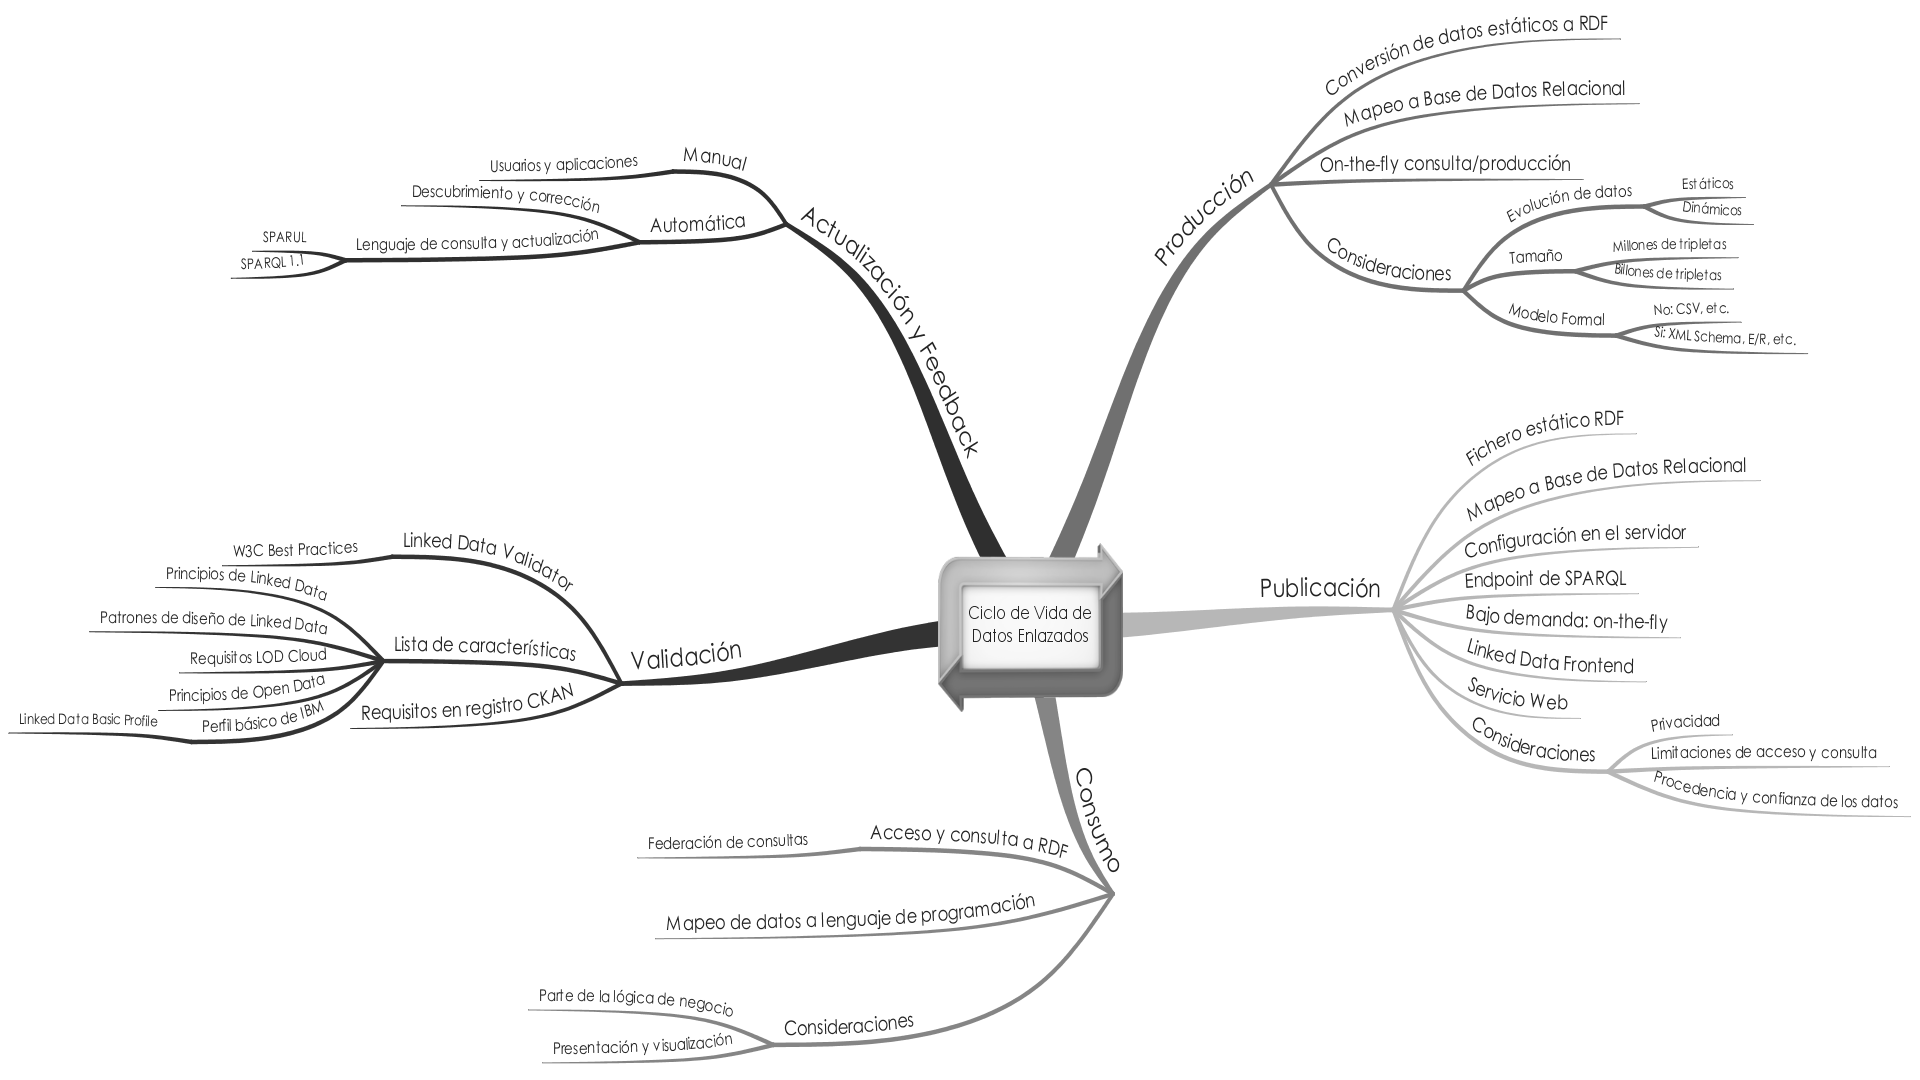
\includegraphics[width=16cm]{images/phd/ldl}
\caption{\textit{Clasificación de Métodos Semánticos}.}
\label{fig:metodos-clasificacion}
\end{figure}

Para llevar a cabo una nueva definición se necesita precisar qué procesos se deben contemplar en la apertura y enlazado
de datos, una vez definidos se identifican los métodos que se pueden aplicar y dentro de los mismos las tareas a ejecutar. 
Por ejemplo, en el proceso de ``Producción'' se deberá identificar los datos a transformar, seleccionar un esquema de URIs y validar la transformación. 
Por lo tanto, se cuenta con una descripción de tres niveles: proceso, método semántico y tarea, que intenta dar respuesta a las siguientes preguntas, ver Tabla~\ref{tabla:procesos}. La selección
de estos procesos, métodos y tareas se ha llevado a cabo tratando de factorizar las actividades presentes en los distintos ciclos de vida de los datos enlazados.

\begin{longtable}[c]{|p{6cm}|p{8cm}|} 
\hline
  \textbf{Proceso} &  \textbf{Pregunta} \\\hline
\endhead
Producción & ¿Qué datos y cómo los transformo? \\ \hline
Publicación & ¿Cómo publico los datos transformados? \\ \hline
Consumo & ¿Cómo reutilizo los datos enlazados disponibles? \\ \hline
Realimentación & ¿Cómo actualizo y mejoro mis datos enlazados? \\ \hline
Validación & ¿Cómo verifico que los datos enlazados en los distintos procesos son correctos? \\ \hline
\hline
\caption{Procesos y Preguntas en \linkeddata.}  \label{tabla:procesos}\\    
\end{longtable}


El proceso a seguir para desarrollar este capítulo es el siguiente:
\begin{enumerate}
 \item Definir los métodos semánticos de forma general en el marco de un proceso.
 \item Explicar los distintos enfoques que dan respuesta a ese método.
 \item Comentar las tareas que implica llevar a cabo el enfoque anterior.
 \item Ejemplificar el método con un ejemplo transversal.
\end{enumerate}

\begin{figure}[!htb]
\centering
	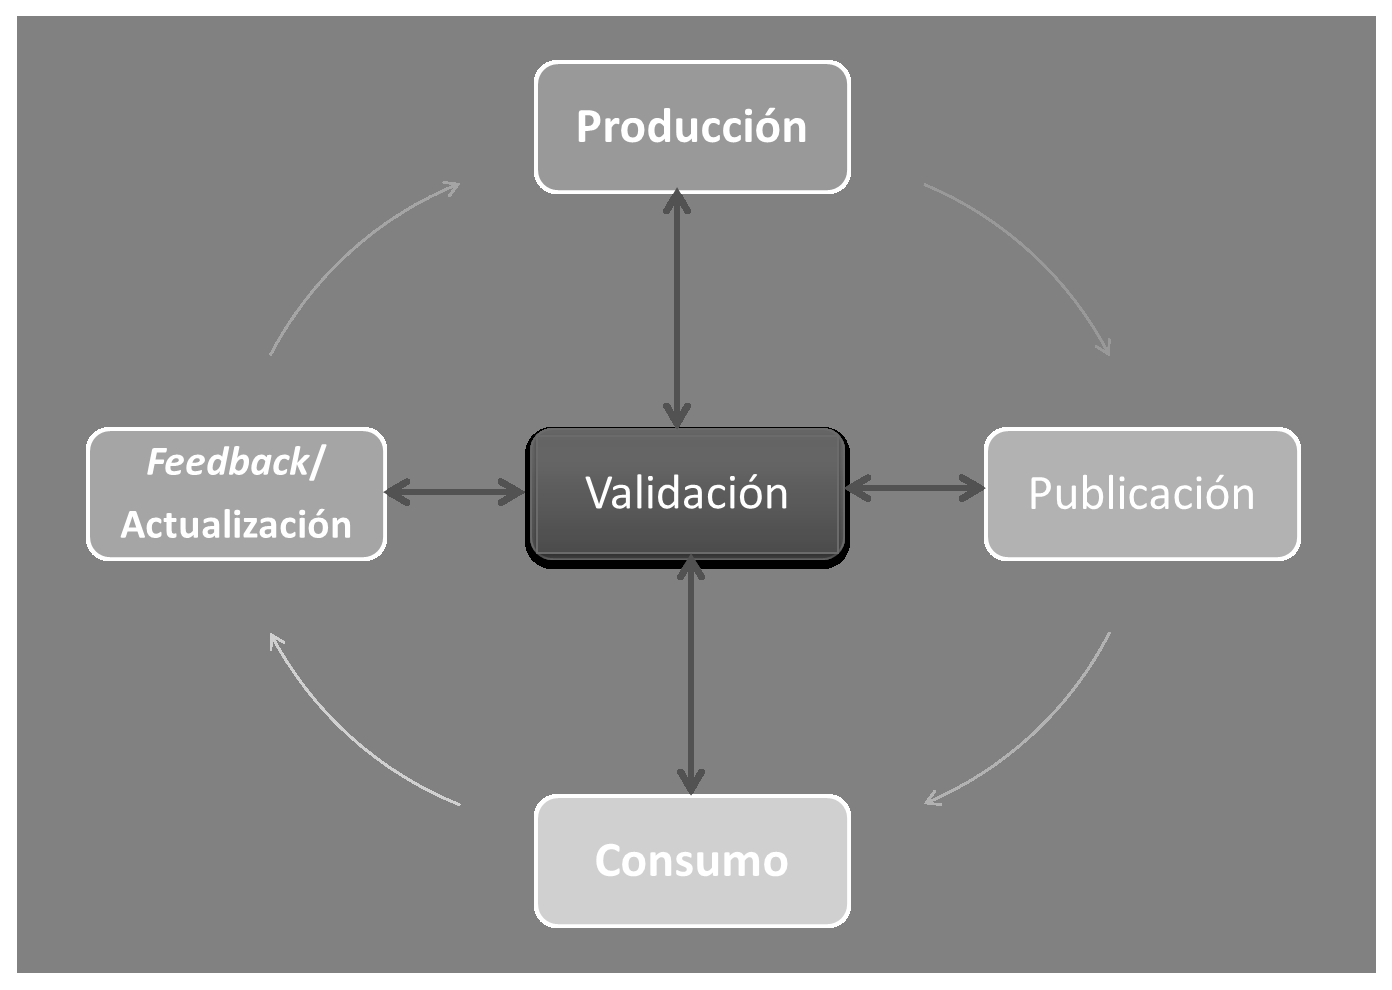
\includegraphics[width=14cm]{images/phd/lld}
\caption{Procesos en \linkeddata.}
\label{fig:metodos-clasificacion-2}
\end{figure}


\subsection{Ejemplo transversal}
Para ejemplificar cada una de las definiciones realizadas a lo largo de este capítulo se utilizará
un ejemplo de un conjunto de datos real. Se ha seleccionado la información disponible en el Nomenclátor
de Asturias 2010 realizado por la Sociedad Asturiana de Estudios Económicos e Industriales, ya que contiene
información de distintos ámbitos (nombres, estadísticas, etc.) e idiomas y facilita la comprensión y lectura del documento. 

\section{Definiciones Previas}
Durante este capítulo se utilizarán algunas de las definiciones ya realizadas
en las distintas especificaciones~\cite{RDF,citeulike:1556975,RDFS,owl2-primer,SparqlSemantics,Perez:2009:SCS:1567274.1567278} sobre el uso de Web Semántica y algunos
de los conceptos clave pertenecientes a la iniciativa de \linkeddata. 

\begin{description}

 \item [Tupla.] Siguiendo las definiciones utilizadas en el modelo relacional y en matemáticas, una tupla
es una función que \textit{mapea} nombres con valores. En general, se trata de un conjunto de valores
$a_1,a_2...a_n$ que guardan una relación de orden entre sí, pueden contener valores repetidos y otros objetos dentro de sí.

\item [\textit{Dataset}.] Se puede definir como un conjunto de tuplas. Si se tiene en cuenta que en la mayoría de los
casos al producir \linkeddata los datos se obtienen de una base de datos relacional, \gls{XML}, texto separado por comas, etc., cada uno de los almacenes especifican una forma de guardar tuplas para generar un \dataset.

\item [\textit{Internationalized Resource Identifiers} (\gls{IRI}s).] Habitualmente se utiliza la denominación de IRI (\gls{RFC}-3987) para referirse
a una generalización de las \gls{URI}s y URLs (RFC-3986), siendo totalmente compatibles con las definiciones de las anteriores. 
Normalmente se presentan de la siguiente forma $<IRI>$ y pueden ser relativas respecto a un IRI base o completas.

En las definiciones formales de \gls{RDF} y \gls{SPARQL} se utiliza el término IRI pero por su definición puede ser utilizado
también el término URI. En el ámbito de \linkeddata se puede afinar aún más y utilizar la siguiente nomenclatura:
 $IRI \longrightarrow  URI \longrightarrow  HTTP$ $URI$.

\item [\textit{Uniform Resource Identifier}.] El concepto de URI surge como una cadena de caracteres para identificar de manera única
a un elemento, en el contexto de la Web Semántica se ha utilizado este término para identificar recursos. Dentro
de la definición de URI encaja \textit{Uniform Resource Locator} (\gls{URL}), que además de proveer información de nombrado sobre el elemento
especifica cómo se ha de acceder a él. En el documento~\cite{RDF} se hace referencia al término HTTP URIs para identificar
a aquellas URIs que utilizan el esquema de nombrado \gls{HTTP} para identificar a los recursos dentro de la iniciativa de la Web Semántica.

\item [Modelo RDF.] Aunque ya se ha comentado en la Sección~\ref{semantica} el modelo RDF, cabe recordar su definición, RDF
sigue y cumple con los principios y características de interoperabilidad, extensibilidad, capacidad de evolución
y descentralización elaborados por el \gls{W3C}. En particular, el modelo RDF se diseñó para tener un modelo de datos
simple con una semántica formal y capacidades de inferencia basado en un vocabulario que hace uso de URIs para nombrar
a los elementos. En el universo RDF, los elementos a modelar son un conjunto de recursos, en esencia todo
aquello que sea susceptible de tener un URI. El lenguaje utilizado para describir estos recursos se compone
de un conjunto de predicados (binarios). Las descripciones de recursos en RDF se basan en la estructura
$<s,p,o>$ (sujeto, predicado, objeto), en los cuales los predicados y los objetos son también recursos o 
literales (en el caso de los objetos). Por otra parte, sujetos y objetos pueden ser anónimos, así tienen URI
pero sólo de forma local, formando lo que se denominan \textit{blank nodes} cuyo uso se ha evaluado y juzgado~\cite{DBLP:conf/semweb/MalleaAHP11} 
recientemente.

En conclusión el modelo RDF consta de unos principios para construir un vocabulario 
bajo una determinada semántica, en muchos casos RDFS~\cite{RDFS} u \gls{OWL}~\cite{owl2-primer}, permitiendo así la herencia
de clases y propiedades, definición de tipos y otras características. Este modelo
es especificado en una serie de documentos que cubren su semántica, sintaxis, serilización, etc.

\item [Tripleta RDF.] Es una tupla $(s,p,o) \in (I \cup B) \times I \times 
(I \cup L \cup B)$, en la que $I$ es el universo de todos los posibles recursos que se pueden identificar
por un IRI, $B$ es un conjunto infinito de recursos no nombrados y $L$ es el conjunto
de todos los literales RDF.

\item [Grafo RDF.] Un conjunto de tripletas RDF se interpreta estructuralmente como un grafo
RDF $\mathcal{G} =(V,E)$, donde $V$ es el conjunto de vértices, $V \subseteq (I \cup B \cup L)$,
y $E$ es el conjunto de ejes, $E \subseteq V \times I \times 
V$. Para cada tripleta $(s,p,o)$ del modelo RDF existe
una arista dirigida, etiquetada con el predicado $p$, entre los vértices que representan el sujeto $s$ y el objeto $o$. Si este
grafo no tiene nodos en blanco se denomina \textit{ground}.

\item [Recurso RDF.] Es un conjunto de sentencias o tripletas $(s,p,o)$ RDF, en las que el sujeto $s$ 
es constante, tiene la misma IRI.

\item [Grafo RDF nombrado.] Es un grafo RDF identificado por un IRI. 

\item [\textit{Dataset} RDF.] En la especificación de SPARQL~\cite{Sparql} y su semántica~\cite{SparqlSemantics} se habla
de \dataset RDF y se define como un conjunto $\mathcal{D} = \{\mathcal{G}, (<I_1>, \mathcal{G}_1), (<I_2>, \mathcal{G}_2)...(<I_n>,\mathcal{G}_n)\}$,
donde $\mathcal{G}$ y cada $\mathcal{G}_i$ son grafos RDF identificados a través de un IRI $I_i$ y $n\geq0$.
 Cada par $(<I_n>, \mathcal{G}_n)$ es un grafo nombrado, en el cual $I_n$ es el identificador del grafo
$\mathcal{G}_n$; $\mathcal{G}$ es el grafo por omisión (\textit{default graph}) y contiene
todas las tripletas. 

Esta definición sobre un \textit{Dataset} RDF se puede extender para definir un modelo formal que sirva
para integrar información proveniente de distintas fuentes de datos dentro de un
repositorio RDF u otro sistema de almacenamiento. Un \dataset integra varios grafos RDF
$\mathcal{G}$, de forma que cada una de las tripletas se puede identificar, gestionar y referenciar
de forma separada. En el modelo de datos de RDF, utilizando grafos nombrados las sentencias forman parte del conjunto de datos o de un 
grafo nombrado $\mathcal{G}_n$ o bien del grafo por omisión $\mathcal{G}$.

Por lo tanto, un \dataset RDF puede representar información de distintos grafos RDF, si se añade
una nueva dimensión a la definición de tripleta RDF $(s,p,o,\mathcal{G})$ se obtienen 
``sentencias contextualizadas'', en las que los tres primeros elementos $(s,p,o)$ indican
una sentencia RDF y el cuarto elemento $\mathcal{G}$ representa el grafo en el que están
definidas. De esta forma un \textit{Dataset} RDF consta de un conjunto infinito de cuádruplas $(s,p,o,\mathcal{G})$. 
Esta definición es ampliamente utilizada en los repositorios RDF para identificar los distintos recursos y así
poder acceder mediante SPARQL a los recursos definidos en determinados grafos.


\item [Ontología.] Se define una ontología $\mathcal{O}$ como una tupla $\mathcal{C}$, $\mathcal{R}$, $\mathcal{I}$, $\mathcal{A}$, donde $\mathcal{C}$ es un conjunto de conceptos,  $\mathcal{R}$ es un conjunto de relaciones, $\mathcal{I}$ es un 
conjunto de instancias y  $\mathcal{A}$ es un conjunto de axiomas. Todos los conceptos, relaciones, instancias
y axiomas se expresan a través de un lenguaje como OWL o F-Logic que permite expresar un determinado formalismo lógico. 
Esta visión de una ontología encaja con la definición realizada en OKBC, los conceptos se corresponderían con clases en OKBC, relaciones con ``slots'', ``facets'' con tipos de axiomas y los ``individuals'' 
corresponderían con instancias.

La necesidad de definir el concepto de ontología reside en que las descripciones de recurso en RDF deberán
haber sido modeladas previamente de acuerdo a un modelo formal. Teniendo en cuenta que en el contexto objeto de estudio se utilizarán
ontologías, un recurso RDF se presenta como una instancia de un concepto de una ontología $\mathcal{O}$ que 
especifique el conocimiento de este dominio.

\item [\textit{Mapeo} entre instancias.] Los \textit{mapeos} entre conceptos e instancias de una ontología $\mathcal{O}$ y en consecuencia
de recursos RDF han sido ampliamente estudiados~\cite{NM00} en el campo de los servicios web semánticos para dar respuesta a
los procesos de mediación. En~\cite{Bruijin2006} se especifican tres operaciones: \textit{mapping}, \textit{alignment} y \textit{merging}, 
como tareas necesarias para realizar el proceso de mediación entre ontologías. En el caso que nos ocupa
es necesario realizar operaciones de \textit{alignment} para identificar recursos RDF similares a uno dado y poder establecer
relaciones de equivalencia, igualdad y \textit{mapeo} en general, por ejemplo, utilizando propiedades como \texttt{owl:sameAs}, \texttt{skos:exactMatch}, 
etc. En el ámbito de \lod se engloban estas técnicas en un problema denominado ``Reconciliación de Entidades'' y además de los
enfoques basados en alineación de instancias de ontologías, se han realizado otros basados en
procesamiento de lenguaje natural de descripciones textuales~\cite{Serimi} o basados en la comparación de URIs~\cite{Maali_Cyganiak_2011}.
 En cualquier caso, es conveniente definir que se entiende por \textit{alignment} en Web Semántica.

\textit{Ontology alignment} es el proceso de descubrir similaridades entre
dos ontologías, el resultado de la operación es una especificación de similaridades
entre las dos ontologías seleccionadas, generalmente este proceso se basa en la aplicación
del algoritmo \textit{Match operator}.

\end{description}


\section{Definición Genérica de Método Semántico}
En primer lugar, debe definirse qué se entiende por método semántico en general y concretamente en el contexto
de este trabajo.

\begin{definition}[Proceso $p$]
Se define un proceso $p$, como la aplicación de uno o varios métodos semánticos. 
\end{definition}


\begin{definition}[Método Semántico $sm$]
Se define un método semántico $sm$, como la consecución de $n$ tareas para llevar a cabo
una operación sobre un \dataset. 
\end{definition}

Este \dataset puede ser un conjunto de valores y datos $\mathcal{G}$, o bien
un \dataset \gls{RDF} $\mathcal{D}$, dependiendo del proceso concreto.

\begin{definition}[Tarea $t$]
 Es cada uno de los pasos que se han de llevar a cabo para realizar un método semántico
\end{definition}


En definitiva, un proceso $p$ dentro de la iniciativa de \linkeddata se puede realizar a 
través de distintos métodos semánticos $sm$, que conlleva a su vez la ejecución de $n$ tareas $t$, implementadas mediante 
diferentes herramientas. De esta forma se puede responder a las preguntas formuladas en la Tabla~\ref{tabla:procesos} y 
que a continuación se ejemplifican.

\begin{Frame}
En el proceso $p$ de ``Publicación'' se puede utilizar un \textit{endpoint de SPARQL} ($sm$) para publicar
los datos y para ello se necesita: $t_1$-disponer de un \dataset RDF $\mathcal{D}$, $t_2$-\textit{desplegar un endpoint de SPARLQ} y 
$t_3$-insertar el \dataset RDF $\mathcal{D}$ en el \textit{endpoint de \gls{SPARQL}}. 
\end{Frame}

En este caso, para una mayor precisión se podría utilizar por ejemplo un interfaz web para insertar los datos 
o bien una consola, un \textit{script}, etc., pero no es necesario especificar hasta ese nivel de detalle ya que 
dependería de las herramientas utilizadas para cada caso.

\section{Relación con Modelos de Ciclo de Vida}
Los modelos de ciclo de vida definen las distintas fases o pasos a realizar para la apertura
y gestión de los datos enlazados. En general, se trata de procesos de alto nivel que sirven como guía tanto desde un punto de vista
estratégico como técnico y que crean concienciación de los puntos clave para la apertura y enlazado de datos. En las siguientes
tablas se realiza la alineación de los métodos que se han identificado inicialmente.
\newpage
\begin{longtable}[c]{|p{6cm}|p{8cm}|} 

\hline

  \textbf{Etapa/Fase/Paso} &  \textbf{Proceso} \\\hline

\endhead
\textit{Identify} & Producción \\ \hline
\textit{Model} & Producción \\ \hline
\textit{Name} & Producción \\ \hline
\textit{Describe} & Producción \\ \hline
\textit{Convert} & Producción, Validación \\ \hline
\textit{Publish} & Publicación \\ \hline
\textit{Manteinance} & Realimentación, Producción, Publicación, Consumo \\ \hline
\hline
\caption{Alineación Métodos Semánticos y Ciclo de Vida de Bernadette Hyland}  \label{tabla:metodos-hyland}\\    
\end{longtable}

En este primer ciclo de vida, ver Tabla~\ref{tabla:metodos-hyland}, existe un proceso de sumo interés como es el 
de mantenimiento de los datos generados. Por otra parte, cada uno de los pasos que se describen forman parte de un modo 
más específico de tareas a realizar para la producción y publicación de datos. En el contexto que nos ocupa, 
se entiende un método semántico como una función que realiza una transformación de datos, con un 
objetivo dentro de un ámbito de un proceso de mayor orden como producción, publicación o consumo. Por ello, este primer ciclo de vida describe las tareas a realizar y no los métodos semánticos, ni los procesos de alto nivel.

\begin{longtable}[c]{|p{6cm}|p{8cm}|} 

\hline

  \textbf{Etapa/Fase/Paso} &  \textbf{Proceso} \\\hline

\endhead
\textit{Data Awareness} & Producción \\ \hline
\textit{Modelling} & Producción y Validación \\ \hline
\textit{Publishing} & Publicación \\ \hline
\textit{Discovery} & Producción, Publicación, Consumo, Realimentación \\ \hline
\textit{Integration} & Producción \\ \hline
\textit{Use Cases} & Consumo  \\ \hline
\hline
\caption{Alineación Métodos Semánticos y Ciclo de Vida de Michael Hausenblas}  \label{tabla:metodos-hausenblas}\\    
\end{longtable}

Al igual que en el modelo de ciclo de vida anterior, la versión propuesta por Michael Hausenblas, ver Tabla~\ref{tabla:metodos-hausenblas}, identifica actividades
a llevar a cabo que no están enclavadas en un proceso de mayor calado y que pueden ser comunes a varias de las
fases. En este ciclo de vida cabe resaltar dos fases como la de \textit{Integration} y \textit{Use Cases} ya que
esto significa que proporciona un enfoque totalmente orientado a la explotación, en realidad se puede considerar como 
parte del proceso de consumo de datos.

\begin{longtable}[c]{|p{6cm}|p{8cm}|} 

\hline

  \textbf{Etapa/Fase/Paso} &  \textbf{Proceso} \\\hline

\endhead
\textit{Specification} & Producción \\ \hline
\textit{Modelling} & Producción y Realimentación \\ \hline
\textit{Generation} & Producción y Validación \\ \hline
\textit{Publication} & Publicación \\ \hline
\textit{Exploitation} & Consumo y Realimentación \\ \hline
\hline
\caption{Alineación Métodos Semánticos y Ciclo de Vida de Boris Villazón-Terrazas}  \label{tabla:metodos-boris}\\    
\end{longtable}

Las fases establecidas por Boris Villazón, ver Tabla~\ref{tabla:metodos-boris}, constituyen una buena guía con procesos
de un mayor grado de abstracción que no indican exactamente los pasos a realizar para su consecución, nuevamente se
hace hincapié en la explotación de los datos enlazados como parte esencial de esta iniciativa.

\begin{longtable}[c]{|p{6cm}|p{8cm}|} 

\hline

  \textbf{Etapa/Fase/Paso} &  \textbf{Proceso} \\\hline

\endhead
\textit{Selection} & Producción \\ \hline
\textit{Conversion} & Producción y Validación \\ \hline
\textit{Publication} & Publicación \\ \hline
\textit{Interlinking} & Producción \\ \hline
\textit{Exploitation} & Consumo y Realimentación \\ \hline
\hline
\caption{Alineación Métodos Semánticos y \textit{DataLift Vision}}  \label{tabla:metodos-data-lift}\\    
\end{longtable}

La visión del ciclo de vida realizada por \textit{DataLift}, ver Tabla~\ref{tabla:metodos-data-lift}, utiliza
un enfoque similar a las definiciones provistas en este documento sobre procesos, pero no tiene en cuenta directamente ni la realimentación, ni el control
de la calidad como parte necesaria del proceso de promoción de datos a la iniciativa de \linkeddata.

\begin{longtable}[c]{|p{6cm}|p{8cm}|} 

\hline
  \textbf{Etapa/Fase/Paso} &  \textbf{Proceso} \\\hline

\endhead
\textit{Interlinking/Fusing} & Producción \\ \hline
\textit{Classification/Enrichment} & Producción \\ \hline
\textit{Quality Analysis} & Producción \\ \hline
\textit{Evaluation/Repair} & Producción y Validación \\ \hline
\textit{Search/Browsing/Exploration} & Publicación \\ \hline
\textit{Extraction} & Consumo \\ \hline
\textit{Storage/Querying} & Consumo y Realimentación \\ \hline
\textit{Manual revision/Authoring} & Validación y Realimentación \\ \hline
\hline
\caption{Alineación Métodos Semánticos y Ciclo de Vida de LOD2 Project}  \label{tabla:metodos-lod2}\\    
\end{longtable}

El trabajo desarrollado en el proyecto LOD2, ver Tabla~\ref{tabla:metodos-lod2}, establece además
de procesos, ciertas tareas clave para el éxito del consumo de los datos publicados. También
es conveniente resaltar que por primera vez se establece la necesidad de validación manual en determinadas tareas.

\begin{longtable}[c]{|p{6cm}|p{8cm}|} 

\hline

  \textbf{Etapa/Fase/Paso} &  \textbf{Proceso} \\\hline

\endhead
\textit{Contextualization} & Producción y Realimentación \\ \hline
\textit{Ontology Design} & Producción y Realimentación \\ \hline
\textit{RDF Graph Modelling} & Producción, Realimentación \\ \hline
\textit{SPARQL endpoint implementation} & Publicación \\ \hline
\textit{RDF Graph implementation} & Publicación \\ \hline
\textit{Update Graph Service} & Realimentación \\ \hline
\textit{Documentation} & Consumo \\ \hline
\textit{Data Visualization Tool} & Consumo \\ \hline
\hline
\caption{Alineación Métodos Semánticos y Metodología BCN y Universidad de Oviedo}  \label{tabla:metodos-bcn}\\    
\end{longtable}

La metodología y proceso de adopción, ver Tabla~\ref{tabla:metodos-bcn}, desarrollada por la Universidad de Oviedo en conjunción con la 
Biblioteca del Congreso de Chile fija las tareas a desarrollar circunscribiéndose a un contexto concreto, la documentación 
oficial que emana de la actividad propia del Congreso de Chile, estos destacan especialmente por dos etapas: el servicio de actualización de datos
y la documentación.

En general, la experiencia de estos ciclos de vida y metodologías de adopción de \linkeddata y \lod se centran
en las tareas a desarrollar y suelen coincidir en su orientación, aunque no es un nombrado. Sin embargo,
no se contemplan tareas como la revisión de la calidad de los datos o la privacidad (esto es cuestionable refiriéndose a \lod), 
es por ello que la factorización realizada en distintos procesos de mayor nivel de abstracción, permite aislar 
las operaciones y realizar una separación de responsabilidades. Sin constituir un objetivo la obtención de un nuevo 
YALDC (\textit{Yet Another Linked Data Life Cycle}) evidentemente a efectos de organización de las tareas realizadas
en la aplicación de \linkeddata en el ámbito de las licitaciones públicas, se ha decido utilizar el enfoque
que se describe en este capítulo. Además, la novedad de estos ciclos de vida, surgidos desde casos prácticos, 
fundamenta la reutilización tanto de la experiencia de sus autores como la propia, para realizar el enfoque desde la teoría a la práctica.


\section{Tareas Comunes en los Procesos de \linkeddata}
Independientemente del proceso, fase o etapa en la que se realicen operaciones con datos enlazados, se presentan 
repetitivamente situaciones susceptibles de subsanación, por ejemplo la identificación de vocabularios a utilizar en el proceso
de producción o de realimentación o cómo diseñar las URIs de los recursos objeto de publicación. Para ello,
en los ciclos de vida que se han repasado en la sección anterior, en los libros, especificaciones y buenas
prácticas de la iniciativa de \linkeddata se encuentran soluciones a estos problemas comunes. El objetivo
de esta sección es presentar algunas de estas tareas para a partir de ellas, construir el método semántico
que implementa un proceso dentro de esta propuesta, para la realización de estas tareas se pueden establecer
una serie de responsables, prácticas y resultados de salida esperados. Tomando como base las metodologías
tradicionales de software como Métrica V3~\cite{mv3}, se definen estos conceptos de forma sencilla y abierta
para su posible ampliación.

\begin{longtable}[c]{|p{6cm}|p{8cm}|} 

\hline
 \textbf{Participante/Rol} & \textbf{Responsabilidad} \\\hline
\endhead
 Propietario de datos & Es el encargado de establecer la estrategia de apertura de datos. Tiene dos perfiles: técnico y de gestión. \\ \hline
 Experto en el dominio & Es el conjunto de personas que se encargan habitualmente de los datos. \\ \hline
 Desarrollador & Es el encargado de llevar a la práctica la iniciativa de \linkeddata sobre los datos escogidos por el \textbf{Propietario}
y modelados por el \textbf{Experto en el domino}. \\ \hline
Usuario final & Beneficiario de la apertura de datos como \linkeddata. Puede ser una persona, entidad, etc., de perfil
técnico o simplemente un usuario de Internet. \\ \hline
\hline
\caption{Participantes/Roles en \linkeddata.}  \label{tabla:users}\\    
\end{longtable}

Esta lista de participantes y responsabilidades, ver Tabla~\ref{tabla:users}, establece una clasificación
sencilla para identificar a los agentes implicados en llevar a cabo la apertura de datos, puede ser más extensa 
incluyendo consultores, analistas, etc., pero el objetivo es determinar de forma intensiva una serie de roles, 
no realizar una descripción extensiva de cada uno de los posibles participantes.


\begin{longtable}[c]{|p{1cm}|p{3cm}|p{3cm}|p{3cm}|p{4cm}|} 

\hline
 \textbf{ID} &   \textbf{Tarea} &  \textbf{Responsables} &  \textbf{Prácticas}  &  \textbf{Resultado} \\\hline
\endhead
$t_1$ & Análisis del \dataset a transformar & Desarrollador, Propietario de datos y Experto en el dominio & Documentación previa, Reunión y Esquemas & Documentación
de especificación inicial \\ \hline
$t_2$ & Limpieza de datos & Desarrollador y Propietario de datos & Documentación previa, Reunión y Catálogos & Conjunto de datos ``limpios''\\ \hline
$t_3$ & Selección de Vocabularios & Desarrollador y Experto en el dominio & Documentación previa, Reunión, Esquemas y Catálogos & Catálogo de vocabularios
candidatos\\ \hline
$t_4$ & Selección de otros \datasets \gls{RDF} & Desarrollador y Experto en el dominio & Documentación previa, Reunión, Esquemas y Catálogos & Catálogo de 
\datasets RDF \\ \hline
$t_5$ & Modelado de datos en RDF  & Experto en el dominio & Documentación previa, Reunión, Esquemas y Catálogos & Ontología
de dominio $\mathcal{O}$ y \dataset RDF $\mathcal{D}$  \\ \hline
$t_6$ & Diseño de un Esquema de \gls{URI}s  & Desarrollador, Propietario de datos y Experto en el dominio & Reunión y Esquemas & Catálogo de URIs y
\dataset RDF $\mathcal{D}$  \\ \hline
$t_7$ & Diseño Plantilla Objetivo del Recurso RDF  & Desarrollador y Experto en el dominio & Reunión y Esquemas & Plantilla recurso RDF \\ \hline
$t_8$ & Enriquecimiento de los datos en RDF  & Desarrollador y Propietario de datos & Reunión y Esquemas & \textit{Datasets} RDF enriquecidos \\ \hline
$t_9$ & Transformación de los datos a RDF  & Desarrollador & Herramienta de generación de datos en RDF (preferible con validación) & RDF \dataset $\mathcal{D}$ \\ \hline
$t_{10}$ & Reconciliación de Entidades  & Desarrollador y Propietario de datos & Reunión y Esquemas & Conjunto $EM$ de tuplas de recursos RDF ponderados \\ \hline
$t_{11}$ & Ponderación de Recursos RDF& Usuario final & Programas de consumo de datos RDF &Conjunto de tuplas $M$ de tuplas $<r_{RDF}, k>$ \\ \hline
$t_{12}$ & Validación de Recursos RDF& Desarrollador, Experto en el dominio y Propietario de datos & Tablas &  Tabla de grado de cumplimiento de características y metainformación\\ \hline
$t_{13}$ &Consolidación de datos RDF & Desarrollador, Experto en el dominio y Propietario de datos& Reunión y Esquemas & \textit{Dataset} RDF consolidado \\ \hline
$t_{14}$ &Infraestructura para \linkeddata& Desarrollador y Propietario de datos & Reunión y Esquemas & Especificación de componentes de infraestructura \\ \hline
$t_{15}$ &Acceso y formato en datos RDF & Desarrollador y Propietario de datos& Reunión y Esquemas & Especificación de despliegue de datos \\ \hline
$t_{16}$ & Añadir metainformación a los recursos RDF& Desarrollador y Propietario de datos & &\textit{Dataset} RDF $\mathcal{D}$ 
enriquecido con metainformación de \provenance y \trust \\ \hline
$t_{17}$ & Documentación extra& Desarrollador, Experto del dominio y Propietario de datos& Reunión, Tablas y Esquemas &Documentación a los procesos realizados \\ \hline

\hline
\caption{Resumen de especificación de tareas.}  \label{tabla:tareas}\\    
\end{longtable}

La ejecución de estas tareas se enclavan dentro de los distintos procesos y métodos del ciclo de vida 
generando un flujo de trabajo, ver Figura~\ref{fig:flujo-tareas-procesos}, en el cual la generación de datos enlazados se convierte en un proceso 
de ingeniería cuantificable delimitado en el cual se pueden establecer métricas de tiempo y esfuerzo 
para la optimización de recursos.

\begin{figure}[!htp]
    \centering
	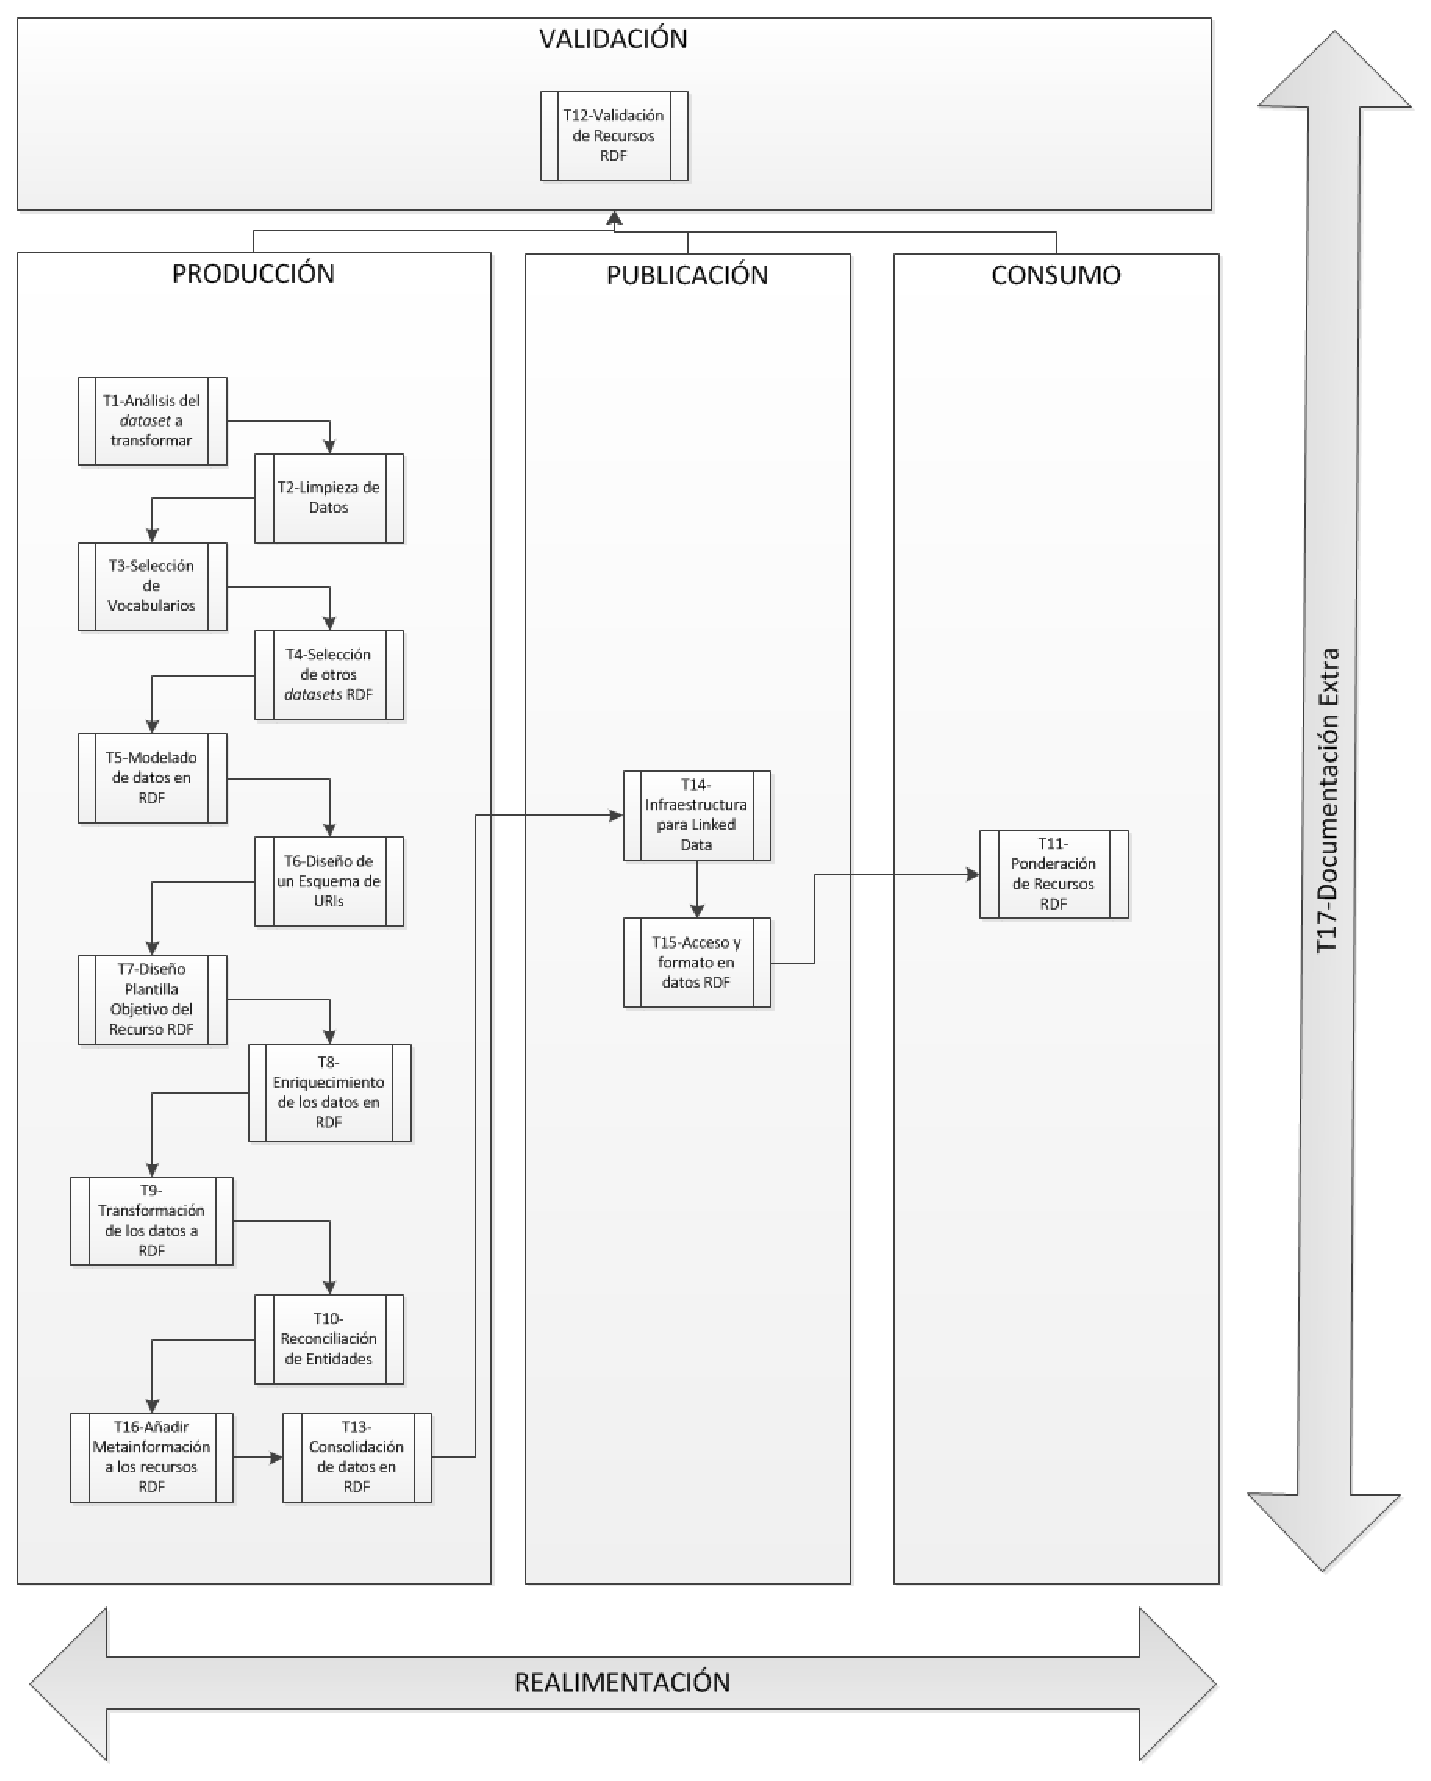
\includegraphics[width=16cm]{images/phd/modelo/flujo-tareas}
	\caption{Flujo de Tareas en los distintos Procesos del Ciclo de Vida de Datos Enlazados.}
	\label{fig:flujo-tareas-procesos}
\end{figure}


\subsection{Tarea $t_1$-Análisis del \dataset a transformar}
Esta tarea conlleva estudiar los datos que se van a transformar, identificando los tipos
de datos a modelar, los conceptos y relaciones que se establecen entre los mismos. También 
hay que tener en cuenta el grado de evolución de los datos, si son dinámicos, es decir si varían a lo largo del tiempo y tienen su 
origen en una base datos, o bien si son estáticos procedentes de un fichero \gls{XML}, \gls{CSV}, etc., y no cambian en un plazo corto de tiempo. 
El resultado de esta tarea será una primera especificación de los datos a modelar, probablemente en lenguaje natural y a 
la cual se le dará soporte formal en la tarea específica de modelado de datos en \gls{RDF}.

La responsabilidad de esta tarea deberá ser la conjunción del esfuerzo entre el \textit{Desarrollador} y el \textit{Propietario de datos}, 
tanto desde un punto de vista técnico como de dominio. Aunque el desarrollador sea capaz de entender los datos que está tratando es necesario conocer el por qué de esos datos, su significado
y la forma de conseguirlos, para ello se pueden utilizar informes previos, entrevistas, etc.

En el ejemplo citado con anterioridad, el Nomenclátor de Asturias 2010 dispone de la siguiente información:
\begin{itemize}
 \item Códigos: 2 cifras para indicar el Concejo (CC), 2 cifras para indicar la Parroquia (PP) y 2 cifras para indicar la entidad de población (EE). La
concatenación de estas 6 cifras da lugar a un identificador único de la entidad de población.
\item Nombre: en español según el Instituto Nacional de Estadística y en asturiano o nombre tradicional.
\item Categoría: existen varias categorías en jerarquía según el tipo de la entidad de población (Concejo, Parroquia, Lugar, Ciudad, Villa, etc.)
\item Datos estadísticos: datos físicos para la altitud, distancia y superficie, número de hombres y mujeres y número de viviendas
principales y no principales.
\end{itemize}

Estos datos se encuentran disponibles en el formato del programa MSExcel y se pueden descargar a través de la página web del SADEI. Una entidad
de población de ejemplo podría ser la siguiente, ver Tabla~\ref{tabla:ejemplo-datos}, también existen algunas peculiaridades dependiendo
del tipo de población, por ejemplo los concejos no tienen altura, por lo que habría que tomar la máxima o la mínima de sus entidades
de población o bien descartar el uso de este valor en las entidades que no lo posean.


\begin{longtable}[c]{|p{8cm}|p{4cm}|} 

\hline

  \textbf{Dato} &  \textbf{Valor} \\\hline

\endhead
Código Concejo & 53 \\ \hline
Código Parroquia & 08 \\ \hline
Código Entidad & 02 \\ \hline
Nombre & Llanuces \\ \hline
Nombre Tradicional & Chanuces \\ \hline
Tipo de Entidad & Lugar \\ \hline
Superficie $km^{2}$ & 7 \\ \hline
Altitud $m$ & 870 \\ \hline
Habitantes & 28 \\ \hline
Hombres & 17 \\ \hline
Mujeres & 11 \\ \hline
Viviendas & 59 \\ \hline
Viviendas Principales & 15 \\ \hline
Viviendas No Principales & 44 \\ \hline
\hline
\caption{Ejemplo de entidad de población en el Nomenclátor de Asturias 2010.}  \label{tabla:ejemplo-datos}\\    
\end{longtable}

\begin{figure}[!htp]
\begin{lstlisting}
"53","08","02","Llanuces","Chanuces","Lugar",,"7,00",870,28,17,11,59,15,44
\end{lstlisting}
	\caption{Ejemplo de entidad de población en el Nomenclátor de Asturias 2010 en formato CSV.}
	\label{fig:ejemplo-datos-csv}
\end{figure}


\subsection{Tarea $t_2$-Limpieza de Datos}
La necesidad de esta tarea surge por la posibilidad de que las fuentes de datos a promocionar a la iniciativa de \linkeddata
dispongan de valores extraños o corruptos que no deberían formar parte del \dataset final. Esta tarea
denominada \textit{Data Cleansing} es de vital importancia para asegurar que los datos generados cuentan con la calidad suficiente para
ser reutilizados por terceros y no arrastrar valores incorrectos desde las fuentes originales. En realidad, adicionalmente
cuando se realiza esta tarea se hace un proceso de depuración de datos que en muchos casos sirve para mejorar no sólo los 
datos publicados sino los datos procedentes de la fuente original.

El responsable de realización de esta tarea será el \textit{Desarrollador} y el \textit{Propietario de datos}, como resultado se obtendrá
un conjunto de datos inicial con valores correctos.

En el caso del Nomenclátor de Asturias se producía la situación de que en cada tupla existía un carácter blanco extra
en cada uno de los códigos, que no tiene ningún sentido para la generación final de datos, además otras cuestiones referidas al 
uso de minúsculas o mayúsculas no estaba unificado, por lo que la limpieza de estos datos para que sigan un convención
como ``\textit{Camel Case}'' o similar facilita posteriormente su transformación de forma correcta.


\subsection{Tarea $t_3$-Selección de Vocabularios}
Una vez identificadas las entidades y las relaciones de un dominio, es conveniente
reutilizar los vocabularios que dan soporte para realizar estas definiciones y descripciones. El abanico
de las posibilidades es muy amplio y existen diversas fuentes de consulta que mantienen una lista
de los vocabularios más utilizados según el dominio: bibliografía, salud, etc. Debe atenderse 
a la existencia de estas especificaciones e intentar impulsar la reutilización de conocimiento e información en 
su máxima expresión. 

La responsabilidad de esta tarea deberá ser un esfuerzo conjunto entre el \textit{Desarrollador} y un \textit{Experto en el dominio} a 
modelar. El resultado de esta tarea debe ser una especificación de los vocabularios candidatos
a ser reutilizados incluyendo la posibilidad de extensión de los mismos.

Siguiendo con el ejemplo citado, se identifica la necesidad de modelar las relaciones entre las entidades y por consiguiente, los vocabularios
apropiados para ello podrían ser los siguientes:
\begin{itemize}
 \item Información multiling\"{u}e, geográfica y estadística. La información multiling\"{u}e esta implícita
en \gls{RDF}, en cuanto a la geográfica, expresamente no se dispone de datos, pero podría obtenerse la georreferenciación de los
lugares y emplear el vocabulario básico del \gls{W3C} para albergar los datos geográficos, también existen otros vocabularios como el provisto por la iniciativa 
\textit{GeoLinkedData}. Finalmente cabe citar que el vocabulario\textit{RDF Data Cube} se ha desarrollado para la expresión de datos estadísticos.
 \item Jerarquía de entidades. Se puede valorar el uso de \gls{SKOS} y \gls{SKOS-XL} para la definición de una taxonomía.
 \item Tipos de conceptos: altitud, metros, superficie, kilómetros cuadrados, personas, hombres, mujeres, viviendas, etc. Se pueden reutilizar
las definiciones realizadas en la DBPedia.
\end{itemize}


\subsection{Tarea $t_4$-Selección de otros \datasets RDF}
Al igual que en la tarea anterior, una vez identificados los datos a transformar 
es necesario conocer con qué otros \datasets se pueden enlazar los datos generados. Asumiendo que 
el objetivo final es la obtención de un \dataset \gls{RDF} 5 $\star$, esta tarea deviene fundamental.

La responsabilidad de esta tarea recae de nuevo en el \textit{Desarrollador}, que verificará cómo se
consumen esos datos, con qué datos de los que posee se pueden enlazar los recursos externos y finalmente
el \textit{Experto en el dominio} deberá validar que los \datasets relacionados son adecuados en cuanto a su semántica
y forma.

En el ejemplo citado se identifican los siguientes \datasets a reutilizar:
\begin{itemize}
 \item DBPedia para los conceptos identificados.
 \item GeoLinkedData y \gls{NUTS} para la información geográfica.
\end{itemize}

Para buscar estos \datasets candidatos se dispone de herramientas como \textit{Datacatalogs.org}, \textit{Freebase}, \textit{Sindice}, 
\textit{The Data Hub}, etc., pero en muchos casos por la propia experiencia o consultando \datasets de temática 
similar se consigue averiguar cuáles reutilizar. También, consultando la documentación~\cite{dcat-w3c} de los grupos de trabajo del \gls{W3C} 
se puede obtener una buena guía para la selección de los conjuntos de datos a reutilizar.

\subsection{Tarea $t_5$-Modelado de datos en RDF}
La iniciativa de \linkeddata y \lod no sólo trata de publicar y consumir datos masivamente, en este caso habilitando 
el acceso a la base de datos corporativa, ficheros, etc., sería suficiente. Cada agente interesado en el consumo de datos 
debería investigar qué modelo siguen los mismos, un esquema relacional, \gls{XML Schema} o si simplemente
no siguen ningún modelo o, al menos, no es posible acceder a él. Es por ello que surge la necesidad
de establecer un modelo formal para las entidades, relaciones y datos. Dentro de la Web Semántica el uso
de ontologías está ampliamente asentado y aceptado, por lo que habitualmente en el momento de la publicación de los datos
se incluye una definición formal de los recursos \gls{RDF}. Esta formalización puede
ser implícita, por la reutilización de vocabularios y datos preexistentes, o bien explícita porque se haya creado un modelo particular 
para ese conjunto de datos.

La responsabilidad para la realización de este modelado recae sobre un \textit{Experto en el dominio} de los datos a promocionar
mediante \linkeddata. La salida de esta tarea será una ontología de domino $\mathcal{O}$ para esos datos y 
parcialmente el conjunto $\mathcal{D}$ que define el \dataset RDF.

Con el objetivo de ejemplificar esta tarea, se define una jerarquía en \gls{SKOS} para modelar
los tipos de entidades de población, ver Figura~\ref{fig:modelo-nomen}, y las estadísticas, ver Figura~\ref{fig:modelo-nomen-stats}. Se
trata de una versión parcial ya que este modelado tiene mayor calado, especialmente en la parte referida a estadísticas.

\begin{figure}[!htp]
\begin{lstlisting}
 
<http://purl.org/weso/nomenclator/ontology/Concejo> 
	skosxl:prefLabel "Concejo"@es ;
	rdfs:subClassOf skos:Concept ;
	owl:sameAs <http://dbpedia.org/resource/Municipalities_of_Spain>;
	skos:example <http://purl.org/weso/nomenclator/asturias/2010/resource/01/00/00> ;
	rdfs:label "Concejo"@es .
	
<http://purl.org/weso/nomenclator/ontology/Parroquia> 
	skosxl:prefLabel "Parroquia"@es ;
	rdfs:subClassOf skos:Concept ;
	skos:broaderTransitive <http://purl.org/weso/nomenclator/ontology/Concejo>;
	skos:example <http://purl.org/weso/nomenclator/asturias/2010/resource/01/01/00> ;
	rdfs:label "Parroquia"@es .

<http://purl.org/weso/nomenclator/ontology/Lugar> 
	skosxl:prefLabel "Lugar"@es ;
	rdfs:subClassOf skos:Concept ;
	owl:sameAs <http://dbpedia.org/resource/Lugar>;
	skos:broaderTransitive <http://purl.org/weso/nomenclator/ontology/Parroquia>;
	skos:example <http://purl.org/weso/nomenclator/asturias/2010/resource/01/02/05> ;
	rdfs:label "Lugar"@es .
...
\end{lstlisting}
	\caption{Modelo parcial de tipos de entidad con SKOS del Nomenclátor de Asturias 2010.}
	\label{fig:modelo-nomen}
\end{figure}

Atendiendo a las definiciones formales de una ontología se obtendría la siguiente descripción formal:

$\mathcal{O}_{nomenclator}$, donde $\mathcal{C} = \{Concejo, Parroquia...Lugar\}$, $\mathcal{R} = \{skosxl:prefLabel, rdfs:label...skos:broaderTransitive\}$,
e $\mathcal{I}$ es el conjunto de todas las entidades de población.

\begin{figure}[!htp]
\begin{lstlisting}
 
<http://purl.org/weso/nomenclator/stats/ontology/refArea> a rdf:Property, qb:DimensionProperty;
  rdfs:label "Region"@en;
  rdfs:subPropertyOf sdmx-dimension:refArea;
  rdfs:range skos:Concept;
  qb:concept sdmx-concept:refArea 
	

<http://purl.org/weso/nomenclator/stats/ontology/physicaldata/area> a rdf:Property, qb:MeasureProperty
  rdfs:label "Area"@en;
  rdfs:subPropertyOf sdmx-measure:obsValue;
  rdfs:range xsd:decimal .
...
\end{lstlisting}
	\caption{Modelo parcial de datos estadísticos del Nomenclátor de Asturias 2010.}
	\label{fig:modelo-nomen-stats}
\end{figure}


$\mathcal{O}_{nomenclator\_stats}$, donde $\mathcal{C} = \{Region...Sexo\}$, $\mathcal{R} = \{area...refArea\}$,
e $\mathcal{I}$ es el conjunto de todas observaciones estadísticas para cada entidad de población.

\subsection{Tarea $t_6$-Diseño de un Esquema de URIs}
Se trata sin duda de una tarea clave para la correcta publicación y consumo de datos, el espectro de posibilidades
para realizar un esquema de \gls{URI}s contempla muchos factores y deberá dar respuesta, al menos, a las
siguientes preguntas:

\begin{itemize}
 \item ¿Qué tipo de URIs utilizar?, ¿``Slash'' vs ``Hash''?.
 \item ¿``Meaningful URIs'' vs ``ID based URIs''?.
 \item ¿La negociación de contenido forma parte del URI?.
 \item Factores de éxito del uso de ``Cool URIs''.
 \item Control de URIs-``minting \gls{HTTP URI}s'', ¿Referenciables?.
 \item Uso de fechas en URIs. 
 \item URI para los recursos, URI para las definiciones, URI para la descripción del \dataset, etc.
 \item URI para recursos y definiciones. URI base.
 \item \ldots
\end{itemize}

La responsabilidad de este diseño recae sobre el \textit{Desarrollador}, el \textit{Experto en el dominio} y el \textit{Propietario de datos} ya que desde 
un punto de vista estratégico un correcto esquema de URIs sirve como documentación e incita a la reutilización de los datos enlazados. 
El resultado de esta tarea será una especificación de las URIs a utilizar y en consecuencia, el conjunto $\mathcal{D}$ que define un \dataset \gls{RDF} 
deberá quedar perfectamente establecido

En las Figuras~\ref{fig:modelo-nomen} y~\ref{fig:modelo-nomen-stats} ya se había adelantado el diseño de URIs, no obstante, en la Tabla~\ref{table:nomen-uris}, 
se especifican con mayor detalle.


\begin{longtable}[c]{|p{6cm}|p{4cm}|p{4cm}|} 

\hline

  \textbf{Característica} &  \textbf{Decisión}  &  \textbf{Ejemplo} \\\hline

\endhead
Tipo de separador en URI& \textit{Slash} &  \\ \hline
Tipo de URI & ID URI (promocionar nombres en una URI puede perjudicar su accesibilidad y usabilidad) & <base\_uri>/{CC}/{PP}/{EE} \\ \hline
Negociación de Contenido en URI & No & Uso de cabeceras HTTP\\ \hline
Uso de ``Cool URIs''& Si &\\ \hline
URIs referenciables & Si, el dominio está bajo nuestro control. & \url{http://purl.org/weso/nomenclator/asturias/2010/resource/53/08/02}\\ \hline
Uso de fechas & Si, el año 2010 & $\equiv$\\ \hline
URIs para recursos & Si, sufijo \textit{resource} & \url{http://purl.org/weso/nomenclator/asturias/2010/resource/{CC}/{PP}/{EE}}\\ \hline
URIs para definiciones & Si, sufijo \textit{ontology} & \\ \hline
Base URI para recursos & Si & \url{http://purl.org/weso/nomenclator/asturias/2010/resource} \\ \hline
Base URI para definiciones & Si & \url{http://purl.org/weso/nomenclator/asturias/2010/ontology} \\ \hline
URI descripción del \dataset & Si & \url{http://purl.org/weso/nomenclator/asturias/2010/resource/ds} \\ \hline
\hline
\caption{Diseño de un esquema de URIs para el Nomenclátor de Asturias 2010.}  \label{table:nomen-uris}\\    
\end{longtable}

Este esquema de URIs se prolongaría para el uso de estadísticas ya que se modela por un lado, los datos
propios de la entidad de población, y, por otro, las estadísticas. Realmente con este diseño y modelado se estaría definiendo un \dataset RDF con $4$ grafos nombrados: 


$\mathcal{D}_{nomenclator} = \{\mathcal{G}, \\ (<http://purl.org/weso/nomenclator/asturias/2010>, \mathcal{G}_1), \\ (<http://purl.org/weso/nomenclator/asturias/2010/ontology>, \mathcal{G}_2), \\ (<http://purl.org/weso/nomenclator/asturias/2010/stats>,\mathcal{G}_3), \\ (<http://purl.org/weso/nomenclator/asturias/2010/stats/ontology>,\mathcal{G}_4)\}$


\subsection{Tarea $t_7$-Diseño Plantilla Objetivo del Recurso RDF}
La experiencia y la coherencia en la promoción de datos a la iniciativa de \linkeddata conduce
habitualmente a la creación de un \textit{recurso objetivo} que representa una plantilla o esqueleto, que sirve
de guía para la transformación de los datos. Una vez que se ha realizado el proceso de producción, 
este \textit{recurso objetivo} suele desecharse ya que se dispone de miles de ejemplos en los datos ya 
transformados. Sin embargo, se puede dar el caso en el cual no todos los recursos RDF generados tengan
el mismo número de tripletas y en consecuencia, resulte difícil validar si los datos generados son correctos respecto a la 
intención inicial. Es por ello, que la creación de un esqueleto de los recursos RDF durante toda la vida
de los datos puede facilitar las tareas de validación en las cuales se chequean las relaciones que deben
tener cada uno los recursos o el tipo de dato en los literales. Al igual que en la descripción
de un \dataset, se pueden agregar ejemplos de recursos, manteniendo esta
información mediante una plantilla que pudiera ser objeto de consulta bajo una determinada URI. Por ejemplo, 
en el caso de la descripción de \datasets utilizando \gls{voID} se recomienda utilizar una convención 
de nombrado para ello, no obligatorio obviamente, válido para tareas como el descubrimiento
automático. En este caso, se trataría de utilizar un enfoque similar para ``guardar'' la especificación
de nuestros recursos \gls{RDF} y así poder reutilizarla en posteriores procesos.


La responsabilidad de esta tarea recae en el \textit{Desarrollador} y en el \textit{Experto en el dominio}. Como resultado se obtiene un 
recurso RDF ``ideal'' que es el superconjunto de las propiedades utilizadas en nuestros recursos. Se podrían establecer 
varias plantillas por cada \dataset dependiendo del modelado que se haya realizado, para así procurar soporte a distintas plantillas según una jerarquía.

\begin{figure}[!htp]
\begin{lstlisting} 
<http://purl.org/weso/nomenclator/asturias/2010/resource/template>
      <http://www.w3.org/1999/02/22-rdf-syntax-ns#type>
              <http://purl.org/weso/nomenclator/ontology/Lugar> ;
      rdfs:label "Chanuces"@ast , "Llanuces"@es ;
      <http://purl.org/dc/elements/1.1/identifier>
              "53_08_02" ;
      <http://www.w3.org/2004/02/skos/core#broaderTransitive>
              <http://purl.org/weso/nomenclator/asturias/2010/resource/53/08/00> ;
      <http://www.w3.org/2008/05/skos-xl#prefLabel>
              "Chanuces"@ast , "Llanuces"@es .
\end{lstlisting}
	\caption{Plantilla objetivo de un recurso RDF en el Nomenclátor de Asturias 2010.}
	\label{fig:modelo-nomen-template}
\end{figure}

No obstante y utilizando las actuales recomendaciones y con el objetivo de evitar un exceso de sobre-especificación, en el vocabulario 
de descripción de \datasets voID se dispone de una propiedad: \texttt{void:exampleResource} que proporciona soporte a este enfoque.

\subsection{Tarea $t_8$-Enriquecimiento de los datos en RDF}
Esta tarea es posiblemente una de las más relevantes dentro de la iniciativa de \linkeddata ya que su objetivo
es generar los enlaces a otros \datasets existentes, con la consiguiente reutilización de información
y datos. Para la planificación de esta tarea se debe tener en cuenta qué tipo de datos se pretenden 
enriquecer y de acuerdo al catálogo de \datasets preestablecido, llevar a cabo la ejecución
del proceso de enlazado de datos. Los enfoques para realizar esta tarea son principalmente los dos siguientes:
1) manual y 2) automático. En ambos casos, la validación final manual es prácticamente inevitable ya que no se trata de un proceso determinista y puede verse sometido a cambios durante el ciclo de vida
de los datos. Por ejemplo, se supone que las \gls{URI}s de los recursos con los que se enlazan los datos 
perdurarán en el tiempo, pero pudiera ocurrir que se produjera algún cambio en las mismas. Un proceso
automático sería recomendable, sin embargo en algunos casos la actuación manual es mucho más eficiente.

La responsabilidad de esta tarea recae sobre el \textit{Desarrollador} en primer lugar y el encargado de mantenimiento por delegación del 
\textit{Propietario de datos} en segunda instancia. El resultado de esta tarea será el enriquecimiento
del \dataset \gls{RDF}.

Siguiendo con el ejemplo citado y una vez fijados los \datasets a reutilizar se efectúa 
el enlazado de datos a través de relaciones definidas con este propósito, tales como \texttt{owl:sameAs}, \texttt{skos:related \linebreak Match}, etc.

\begin{figure}[!htp]
\begin{lstlisting} 
<http://purl.org/weso/nomenclator/asturias/2010/resource/44/00/00>
      <http://www.w3.org/1999/02/22-rdf-syntax-ns#type>
              <http://purl.org/weso/nomenclator/ontology/Concejo> ;
      rdfs:label "Oviedo"@es , "Uvieu"@ast ;
      <http://purl.org/dc/elements/1.1/identifier>
              "44_00_00" ;
      <http://www.w3.org/2002/07/owl#sameAs>
              <http://geo.linkeddata.es/resource/Municipio/Oviedo> , 
	      <http://dbpedia.org/resource/Oviedo> ;
      <http://www.w3.org/2004/02/skos/core#broaderTransitive>
              <http://nuts.psi.enakting.org/id/ES12> ;
      <http://www.w3.org/2008/05/skos-xl#prefLabel>
              "Oviedo"@es, "Uvieu"@ast .
\end{lstlisting}
	\caption{Ejemplo de entidad RDF enriquecida del Nomenclátor de Asturias 2010.}
	\label{fig:modelo-nomen-template}
\end{figure}

\subsection{Tarea $t_9$-Transformación de datos a RDF}
De acuerdo a la ejecución de las tareas anteriores sobre el análisis 
del \dataset a transformar, la selección del vocabularios, el diseño 
de \gls{URI}s para los recursos, etc., cabe la realización de la transformación 
para la obtención del \dataset $\mathcal{D}$ en \gls{RDF}. Uno de los puntos 
clave para la ejecución de esta tarea consiste en la selección de la 
herramienta a utilizar, para ello se debe dar respuesta a la siguiente pregunta:

¿Se utilizará una herramienta de propósito general (\gls{ETL}) como Google \gls{Refine} o se 
implementará un programa \textit{ad-hoc}?

Dependiendo de las capacidades de la herramienta y la necesidad de realizar otras tareas como 
la reconciliación de entidades pueden convertirse en buenas pistas para la selección de la misma. Igualmente, 
es conveniente que la expresión de las reglas de \textit{mapeo} para cada una de las tuplas de 
entrada y su conversión en RDF sea lo más sencilla posible asegurando que los recursos 
generados son sintácticamente válidos. La implementación de un programa personalizado siempre 
es una posibilidad correcta en el caso de que la casuística de los datos de entrada sea 
muy diversa y no se puedan expresar todas las condiciones en las herramientas de propósito general. Finalmente, 
otro enfoque se centra en aunar las ventajas de cada una de las opciones y realizar la transformación 
inicial con una herramienta de propósito general y el enriquecimiento y validación de los datos en RDF
con un programa personal. 

El resultado de esta tarea es el \dataset RDF $\mathcal{D}$ conteniendo todos los recursos de información 
de la entrada y para los cuales existe una regla de transformación. La responsabilidad, por lo tanto, 
recae sobre el \textit{Desarrollador} en primer lugar y el encargado de mantenimiento por delegación del \textit{Propietario de datos}, 
en segunda instancia. 

\subsection{Tarea $t_{10}$-Reconciliación de Entidades}
El problema sobre el establecimiento de enlaces entre dos recursos \gls{RDF} está siendo
abordado actualmente desde diferentes puntos de vista con el objetivo de facilitar
el enriquecimiento de los datos de forma automática y determinista. Los enfoques
actuales se centran en el procesamiento del lenguaje natural, utilizando
las descripciones de los recursos en propiedades como \texttt{rdfs:label}, similitud
en \gls{URI}s, etc. Las herramientas que se pueden utilizar para este propósito abarcan desde
sistemas de búsqueda como \textit{Sindice}, a \textit{frameworks} completos como \textit{SERIMI}, utilizando
para ello grandes bases de datos como \textit{Freebase}.

Por tratarse de una subtarea del enriquecimiento de datos, la responsabilidad recae sobre el \textit{Desarrollador} 
en primer lugar y el \textit{Encargado de Mantenimiento} por delegación del \textit{Propietario de datos}, en segunda instancia. 

El resultado de esta tarea será un conjunto $EM$ de tuplas $<r_{source}, r_{target}, k>$, donde $r_{source}$ es el 
recurso RDF de entrada para el cual se buscan candidatos y $r_{target}$ es un recurso RDF candidato valorado con un valor $k$.

También, adicionalmente se puede utilizar este tipo de tarea para descubrir entidades similares
y realizar procesos de descubrimiento y análisis de información y datos de forma automática

\subsection{Tarea $t_{11}$-Ponderación de Recursos RDF}
El consumo de datos \gls{RDF} puede requerir el establecimiento de un mecanismo para la obtención de 
un valor acerca del nivel de representatividad de un recurso en un determinado contexto. Básicamente
el enfoque puede determinarse de acuerdo a un conjunto de relaciones y valores de entrada, otorgando 
una ponderación a cada recurso para que pueda ser utilizado en otras tareas.

El responsable de realizar esta tarea será un \textit{Usuario final} como consumidor
de los datos. Se puede aplicar también a la reconciliación de entidades, y en consecuencia 
al enriquecimiento de los datos en RDF. El resultado de esta tarea será un conjunto $M$ de tuplas $<r_{RDF}, k>$, en el 
cual para cada recurso $r_{RDF}$ perteneciente a un \dataset RDF $\mathcal{D}$ se establece un valor $k$ de relevancia.

Esta tarea resulta relevante igualmente para realizar búsquedas sobre un \dataset RDF, ya que
los actuales lenguajes de consulta como \gls{SPARQL} no permiten establecer una prioridad para
el encaje o ``matching'' de tripletas que impide una ordenación de los resultados por relevancia de acuerdo
a ciertos criterios. Algunas herramientas como Virtuoso de OpenLink han implementado este tipo de características, 
pero carecen de especificación formal en las recomendaciones actuales del W3C.

\subsection{Tarea $t_{12}$-Validación de Recursos RDF}\label{lod-t12}
El objetivo final de la exposición de datos con \gls{RDF} debe ser la reutilización de los mismos
para la creación de otras aplicaciones, para ello se deben proveer datos que cumplan ciertas características de acuerdo al modelo establecido. Es por ello
que la validación de los recursos RDF generados debe ser prioritaria para asegurar
la calidad de los datos que se han obtenido, así se puede atender a diferentes criterios:

\begin{itemize}
 \item Deben ser datos RDF correctos en cuanto al estricto cumplimiento de la sintaxis normativa.
 \item Deben ser correctos en cuanto a rango y dominio de los literales
utilizados y previamente definidos en el modelo. Se deben crear instancias del conjunto
$\mathcal{I}$ de la ontología $\mathcal{O}$.
\item Deben proveer la metainformación adecuada para cumplir con los requisitos de confianza (\textit{trust})
y poder conocer su procedencia (\textit{provenance}). En algunos casos, esta información debe estar disponible
en cada recurso individualmente o a nivel de \dataset RDF, dependiendo bien del contexto en el que se vayan
a utilizar o bien con respecto a las características del propio \dataset. Por ejemplo, tratándose de leyes que pueden
tener un sólo identificador y que evolucionan en el tiempo es conveniente que estas características
se fijen a nivel de recurso. En cambio, si todos los datos del \dataset varían en grupo será más conveniente
añadir esta metainformación a nivel del propio \dataset y no multiplicar esta información en cada
uno de los recursos.
\item Dependiendo de las relaciones y propiedades que se hayan establecido se debe asegurar que 
están presentes en todos los recursos.
\item En relación con otras características igualmente recomendables como la licencia de uso, autoría, autenticidad, autorización de uso, el no repudio, etc., 
es necesaria su inclusión dentro del conjunto de metainformación provista con el objetivo de asegurar su consumo en condiciones de fiabilidad.
\end{itemize}

El responsable de la realización de esta tarea será el \textit{Desarrollador}, el \textit{Experto en el dominio} y el \textit{Propietario de datos}. 
El resultado será un conjunto de directrices en el cual se especifique el grado de cumplimiento de cada una de ellas y cómo se verifique 
el mismo.

En el ejemplo que se está desarrollando y acoplando a lo largo de este capítulo se asegura que:
\begin{itemize}
 \item Los datos RDF son válidos porque se han generado con herramientas que producen un RDF válido.
 \item Se sigue el modelo realizado para especificar cada uno de los recursos.
 \item Se añade metainformación, ver Figura~\ref{fig:meta-nomenclator}, sobre el \dataset a nivel del mismo ya que la evolución
y el cambio en los datos se produce a nivel de conjunto.
\end{itemize}

\begin{figure}[!htp]
\begin{lstlisting} 
<http://purl.org/weso/nomenclator/asturias/2010/resource/ds> a void:Dataset ;
	     rdf:type skos:ConceptScheme ;
	     rdfs:label "Nomenclator Asturias 2010"@en ;
             void:dataDump <http://purl.org/weso/nomenclator/asturias/2010/nomenclator-asturias-2010.ttl> ;
             dcterms:title "Nomenclator Asturias 2010" ;
             dcterms:description "RDF data extracted from INE and Sadei" ;
	     dcterms:source <http://www.sadei.com/> ;
	     dcterms:license <http://opendatacommons.org/licenses/by/1.0/> ;
	     dcterms:publisher <http://www.josemalvarez.es/foaf.rdf#me> ; 
    	     dcterms:author <http://www.josemalvarez.es/foaf.rdf#me> ; 
	     dcterms:author <http://www.di.uniovi.es/~labra/labraFoaf.rdf#me> ; 
	     dcterms:contributor <http://purl.org/weso/nomenclator/asturias/2010/resource/contributor/Weso> ;
     	     dcterms:modified "2011-11-10"^^xsd:date ;
	     void:vocabulary skosxl: , skos:  , geo: ;
             void:target <http://purl.org/weso/nomenclator/asturias/2010/stats/resource/ds> ;
             foaf:homepage <http://purl.org/weso/nomenclator/> ;
             void:exampleResource <http://purl.org/weso/nomenclator/asturias/2010/resource/01/00/00> ;
	     void:exampleResource <http://purl.org/weso/nomenclator/asturias/2010/resource/44/00/00> ;
	     void:exampleResource <http://purl.org/weso/nomenclator/asturias/2010/resource/53/00/00> ;
	     skos:hasTopConcept	  <http://purl.org/weso/nomenclator/asturias/2010/resource/01/00/00> ,
	      ...
	      .
<http://purl.org/weso/nomenclator/asturias/2010/stats/resource/ds> a void:Dataset ;
	     rdfs:label "Statistics Nomenclator Asturias 2010"@en ; 
 	     void:dataDump <http://purl.org/weso/nomenclator/asturias/2010/stats/nomenclator-asturias-2010-stats.ttl> ;
             dcterms:title "Statistics Nomenclator Asturias 2010" ; 
             dcterms:description "RDF data extracted from INE and Sadei" ; 
	     dcterms:source <http://www.sadei.com/> ; 
	     dcterms:license <http://opendatacommons.org/licenses/by/1.0/> ;
	     dcterms:publisher <http://www.josemalvarez.es/foaf.rdf#me> ; 
    	     dcterms:author <http://www.josemalvarez.es/foaf.rdf#me> ; 
	     dcterms:author <http://www.di.uniovi.es/~labra/labraFoaf.rdf#me> ;
	     dcterms:contributor <http://purl.org/weso/nomenclator/asturias/2010/resource/contributor/Weso> ;
     	     dcterms:modified "2011-11-10"^^xsd:date ;	
	     void:vocabulary qb: , sdmx-code: , sdmx-dimension: ;
             foaf:homepage <http://purl.org/weso/nomenclator/> ; 
             void:exampleResource <http://purl.org/weso/nomenclator/asturias/2010/stats/resource/physicaldata/altitude/01/00/00> ;
	     void:exampleResource <http://purl.org/weso/nomenclator/asturias/2010/stats/resource/sex/m/01/00/00> ;  
	     void:exampleResource <http://purl.org/weso/nomenclator/asturias/2010/stats/resource/sex/f/01/00/00> ; 
	  

\end{lstlisting}
	\caption{Metainformación del \dataset RDF del Nomenclátor de Asturias 2010.}
	\label{fig:meta-nomenclator}
\end{figure}


\subsection{Tarea $t_{13}$-Consolidación de datos en RDF}
Esta tarea se encarga de proveer nuevos datos al \dataset RDF agregando parte de los datos ya disponibles. El caso
paradigmático ocurre en materia de estadísticas en el que además de las observaciones particulares se pueden
diseñar recursos \gls{RDF} integrando cierta información de alto valor para que no sea necesaria su réplica por 
cada uno de los consumidores. Por lo tanto, esta tarea consiste en la agregación de los datos RDF ya disponibles.

El responsable de esta tarea será el \textit{Desarrollador}, el \textit{Experto en el dominio} y el \textit{Propietario de datos} que seleccionarán
aquellos datos que deben ser agregados con el objetivo de proveer un mejor acceso a los mismos dotando así al \dataset
RDF de mejores características de accesibilidad y usabilidad de los datos, resultando un \dataset RDF extendido.

Dentro del Nomenclátor de Asturias 2010 consta consta una sección dedicada a observaciones estadísticas que siguiendo las especificaciones
para la publicación de datos estadísticos en RDF se pueden agrupar mediante ``\textit{Slices}'', se trataría de un caso de consolidación
de datos. Por ejemplo, se podrían proveer datos que dieran respuesta directamente a preguntas como: ``Número de personas de género masculino en Llanuces en el año 2010''.
En el vocabulario \textit{RDF Data Cube} este tipo de información se modelaría a través de un ``Slice'', ver Figura~\ref{fig:slice-nomen},
 en el cual se tendrían en cuenta 3 dimensiones (género, región y fecha) y una medida (personas).

\begin{figure}[!htp]
\begin{lstlisting} 
nomen-stats: sliceByRegionSex a qb:SliceKey;
  rdfs:label "Slice by region"@en;
  rdfs:comment "Fixed year, region and sex change"@en;
  qb:componentProperty
  nomen-stats:refPeriod; 
 .
nomen-stats: spopulation a
  qb:DataStructureDefinition;
  qb:component
    [qb:dimension nomen-stats:refPeriod; ],
    [qb:dimension nomen-stats:refArea; ],
    [qb:dimension sdmx-dimension:sex; ],
    [qb:measure
    nomen-stats:population; ];
qb:sliceKey nomen-stats: sliceByRegionSex
.
nomen-stats:region/sex a qb:Slice;
  qb:sliceStructure
  nomen-stats: sliceByRegionSex;
  nomen-stats:refPeriod
  <http://reference.data.gov.uk/id/gregorian-interval/2010-01-01T00:00:00/P1Y> ;
  qb:observation
  nomen-obs:region/sex/m/53/08/02, ...
.
nomen-obs:region/sex/m/53/08/02 a qb:Observation;
  qb:dataSet nomen-stats:nomenclator2010;
  nomen-stats:refArea <http://purl.org/weso/nomenclator/asturias/2010/resource/53/08/02> ;
  nomen-stats:refPeriod <http://reference.data.gov.uk/doc/gregorian-interval/2010-01-01T00:00:00/P1Y> ;
  sdmx-dimension:sex sdmx-code:sex-M ;
  sdmx-attribute:unitMeasure <http://dbpedia.org/resource/Person>
  nomen-stats:population 17 ; 
.
\end{lstlisting}
	\caption{Ejemplo de \textit{Slice} en el \dataset RDF del Nomenclátor de Asturias 2010.}
	\label{fig:slice-nomen}
\end{figure}

\newpage

\subsection{Tarea $t_{14}$-Infraestructura para \linkeddata}
La consecución de todos los procesos, métodos y tareas puede reflejarse en una infraestructura
de herramientas que proporcionen soporte desde dos puntos de vista:

\begin{description}
 \item [Completa.] Cubre todos los procesos, métodos y tareas suministrando las herramientas
adecuadas para cada uno de ellos. Los criterios de selección pueden variar dependiendo
del estado de madurez, de los datos a tratar, de las tareas a realizar, etc. En este sentido
la infraestructura definida en \textit{LOD2 project}, ver Sección~\ref{lod2-project}, se puede
considerar como paradigmática.
\item [Parcial.] Cubre alguno de los procesos, métodos o tareas. Por ejemplo, para el proceso
de publicación, se puede establecer una infraestructura especial que no tenga en cuenta ningún
otro proceso y de por hecho la existencia de datos. A continuación y siguiendo el ejemplo que se desarrolla a lo largo de este capítulo se advierte 
un modelo para para la publicación de datos, ver Figura~\ref{fig:deploy-nomenclator}, que 
supone la existencia de datos en un cierto repositorio y que no provee más operaciones
que la de acceso a datos sin realimentación.
\end{description}

El responsable de esta tarea será el \textit{Desarrollador} y el \textit{Propietario de datos} que deberán
resolver, de acuerdo a unas determinadas especificaciones, el conjunto de componentes que den soporte a los datos. La especificación
de este despliegue puede ser una simple lista de componentes o el uso de diagramas UML particulares
para este tipo de procesos, como el diagrama de componentes o de despliegue.

\begin{figure}[!htb]
\centering
	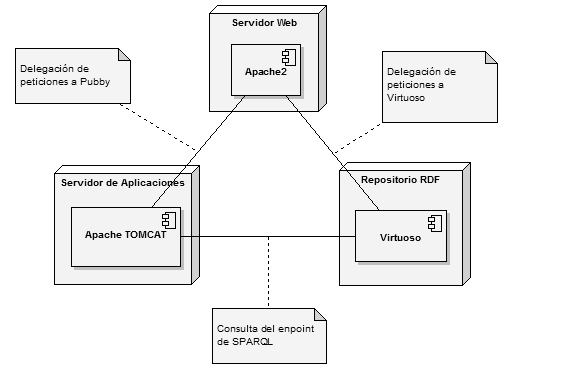
\includegraphics[width=12cm]{images/phd/infra-ld}
\caption{Infraestructura Parcial para el Nomenclátor de Asturias 2010.}
\label{fig:deploy-nomenclator}
\end{figure}

\subsection{Tarea $t_{15}$-Acceso y Formato de datos en RDF}
Seguidamente al proceso de generación de datos en RDF como \linkeddata es necesario establecer
los mecanismos de acceso a la información, en esta tarea se debe dar respuesta a una
serie de cuestiones:
\begin{itemize}
 \item ¿Cómo se va a desplegar la información?, ¿Fichero, repositorio, generación \textit{on-the-fly}, etc.?
 \item ¿En qué formatos se va a ofrecer esta información?
 \item ¿Qué tipo de acceso se va a permitir?, ¿Consulta directa a un \textit{endpoint} de \gls{SPARQL}?, ¿Un servicio web: \gls{REST}, \gls{SOAP}, etc.?
\end{itemize}

La responsabilidad de esta tarea recae en el \textit{Desarrollador} y el \textit{Propietario de datos} que han de decidir 
cómo se ha de hacer pública esta información de acuerdo a la estrategia de la entidad, de la infraestructura tecnológica y de los datos en sí mismos. 
El resultado de esta tarea debe proveer una especificación sobre cómo acceder a los datos en RDF y en qué formatos se van a facilitar.

En el ejemplo que se está desarrollando, se ha decidido la siguiente estrategia:

\begin{itemize}
 \item Despliegue mediante un repositorio semántico con un \textit{endpoint} de \gls{SPARQL} habilitado y ficheros con los volcados completos de los datos.
 \item Los siguientes formatos deben ser prioritarios: \gls{HTML}, \gls{RDF/XML} y \gls{N3}.
 \item Acceso directo a consultar sobre el \textit{endpoint} de \gls{SPARQL} y un servicio de negociación de contenido sobre los datos.
\end{itemize}

\subsection{Tarea $t_{16}$-Añadir metainformación a los recursos RDF}\label{t16-metodos}
El objetivo de esta tarea es dotar a los recursos de información de la metainformación 
necesaria para suministrar soporte a la procedencia de los datos y garantizar 
un cierto grado de confianza en su uso. En esta tarea, existen dos enfoques 
posibles:
\begin{enumerate}
 \item Incluir la metainformación a nivel de \dataset. Esta opción se utilizará cuando 
los recursos tengan un carácter estático y evolucionen poco en el tiempo y en conjunto, de esta forma, 
tiene sentido incluir sólo metainformación a nivel del conjunto completo de datos para no generar 
información superflua.
 \item Incluir la metainformación a nivel de cada recurso. Este enfoque se utilizará cuando 
los recursos tengan un carácter dinámico y evolucionen en el tiempo independientemente de otros 
recursos en el conjunto de datos completo. 
 \item Enfoque híbrido. Evidentemente, si sólo algunos recursos del \dataset son candidatos 
a incluir metainformación a nivel de cada recurso es preferible optar por este enfoque facilitando 
la información donde sea necesaria. La principal desventaja de esta opción reside en que la transformación 
de los datos no es homogénea generando incertidumbre en los posibles clientes. 
\end{enumerate}

La responsabilidad de esta tarea recae en el \textit{Desarrollador} y el \textit{Propietario de datos} que han de decidir 
qué metainformación se debe incluir y qué enfoque aplicar. El resultado de esta tarea es el propio 
\dataset \gls{RDF}, pero incluyendo nuevas tripletas para representar la información necesaria como 
metadatos.

\subsection{Tarea $t_{17}$-Documentación extra}\label{t17-metodos}
Uno de los puntos clave para la reutilización de datos enlazados reside 
en la provisión de una documentación adecuada en relación con el tipo de recursos 
de información que se han transformado y qué datos contienen. Desde un punto 
de vista estratégico las decisiones que se hayan tomado en cuanto a 
selección de vocabularios y otros \datasets a reutilizar, suponen 
una buena guía de documentación facilitando a los clientes datos 
perfectamente conocidos, ahora bien, desde una perspectiva 
operativa es conveniente documentar las decisiones tomadas como el diseño 
de URIs, el tipo de datos utilizado, el acceso a la información, las formas 
de consulta, posibles restricciones, etc., para que la selección del \dataset 
se convierta en una decisión sencilla. Un ejemplo claro de documentación correcta 
es la provista por \textit{GoodRelations} y \textit{ProductOntology} en las cuales 
además de los datos en sí mismos, se ofrecen ejemplos de uso, características, casos 
de éxito en su reutilización, etc., favoreciendo su difusión entre la comunidad.

La responsabilidad de esta tarea recae en el \textit{Desarrollador} y el \textit{Propietario de datos} que han de establecer 
qué partes se pueden documentar públicamente y la forma de difusión la misma, mediante metadatos, etc. El resultado 
de esta tarea será, en general, una especificación de cómo se deben reutilizar los datos. En este sentido, en las últimas 
fechas ha habido una extensa discusión en la lista de correo de \lod en el \gls{W3C} sobre el uso de \texttt{HttpRange-14} para 
consultar cómo se debería incluir información de unos recursos en otros.

El resultado de esta tarea será una serie de documentos de especificación y ejemplos, así como nuevas tripletas \gls{RDF} 
en el \dataset resultado para enlazar esta nueva metainformación.

\section{Proceso de Producción}\label{sect:produccion}

\begin{definition}[Producción]
Proceso que conlleva todas las tareas que implican la transformación de datos a un modelo RDF obteniendo 
como resultado un \dataset \gls{RDF} $\mathcal{D}$.
\end{definition}

\subsection{Método Semántico de Producción de \linkeddata}\label{method-prod-def}
\begin{definition}[Método Semántico de Producción]
$SPM$ es una función que para un conjunto de tuplas de entrada o \dataset $\mathcal{G}$ y un conjunto de \textit{mapeos} $\mathcal{M}$  
genera un \dataset RDF $\mathcal{D}$.
\end{definition}

\begin{center}
    $SPM : \mathcal{G} \times \mathcal{M} \longrightarrow \mathcal{D}$
\end{center}
Las características que tiene esta definición de un $SPM$ son las siguientes:
\begin{itemize}
 \item Para todo valor $g_{i}$ del conjunto de entrada $\mathcal{G}$, existe al menos un
\textit{mapeo} $m_{i}$ en el conjunto $\mathcal{M}$.
 \item Existen valores $g_{i}$ del conjunto de entrada $\mathcal{G}$, para los que existen
varios \textit{mapeos} $m_{i}$ formando un conjunto $\mathcal{M}_{i}$ subconjunto de $\mathcal{M}$.
\end{itemize}

Esta definición implica que toda la información de entrada permanece en el conjunto de salida. Si bien
se podría pensar que existen valores de la entrada, por ejemplo un identificador generado automáticamente desde
una base de datos que no sería candidato a persistir en el conjunto de salida, es conveniente mantener
toda la información por la posibilidad de realizar realimentación y monitorización transversal. Si se apreciara 
la existencia de algún inconveniente con ocasión del consumo o de la publicación se deben proveer otros mecanismos para
hacer transparente esta información.

% La interacción del proceso de producción de datos enlazados junto a otros procesos como el de publicación pueden
% observarse en el diagrama, ver Figura~\ref{fig:produccion} realizado en \textit{Linked Data: Evolving the Web into a Global Data Space}~\cite{Heath_Bizer_2011} según
% el cual se muestran algunos de los métodos utilizados para el proceso de producción de datos enlazados.
% 
% \begin{figure}[!htb]
% \centering
% 	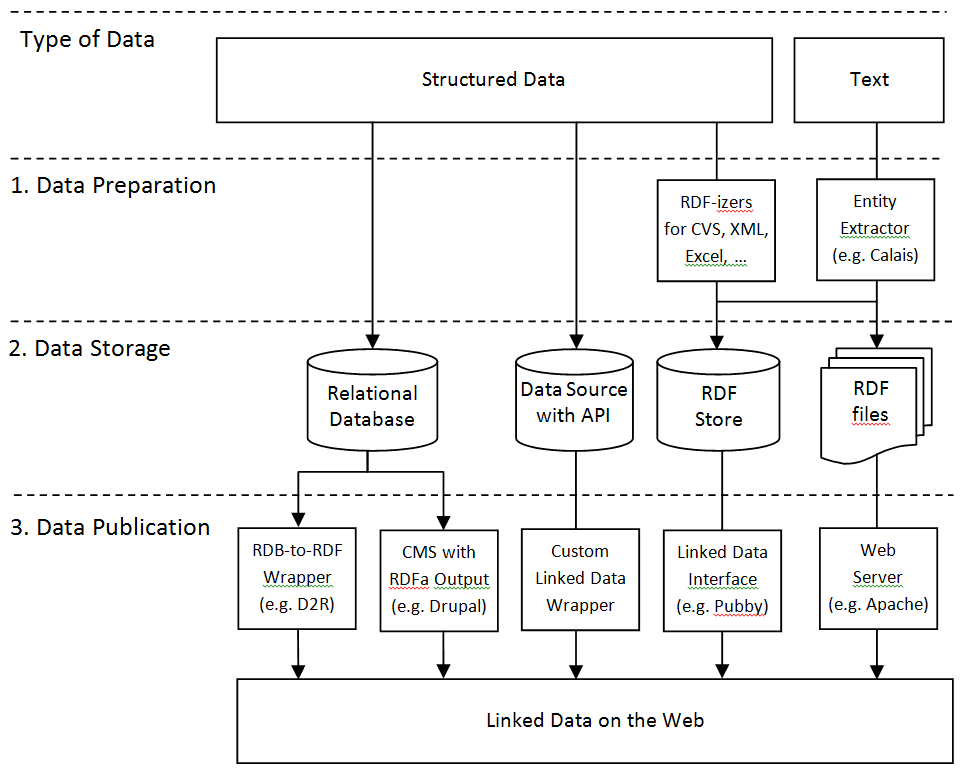
\includegraphics[width=10cm]{images/phd/linkeddata}
% \caption{\textit{Linked Data Publishing Options and Workflows} (extraída de~\cite{Heath_Bizer_2011}).}
% \label{fig:produccion}
% \end{figure}


\subsection{$SPM_1$-Transformación de datos a RDF}\label{spm-1}
Este método de producción de un \dataset \gls{RDF}, $SPM_1$, asume que los datos disponibles se encuentran
en algún formato procesable automáticamente y que en cierto modo son estáticos o bien
es una imagen estática de los mismos. Se trata en concreto del supuesto en el que se dispone de datos en formatos
como \gls{CSV} o MSExcel o bien se hace un volcado de una base de datos para generar posteriormente a partir
de estos valores de entrada el \dataset RDF. 

Por lo tanto, este enfoque se aplicará ante la siguiente situación:
\begin{itemize}
 \item Datos estáticos. Inicialmente sin disponibilidad de acceso mediante un lenguaje de consulta tipo \gls{XPath} o \gls{SQL}.
 \item Formato de datos preestablecido tipo CSV, MSExcel o \gls{XML}.
 \item El tamaño del \dataset de entrada no es excesivamente grande. No existe una forma de evaluar el tamaño
de un \dataset, pero se podría fijar que el resultado final fuera en orden de millones de tripletas RDF.
\end{itemize}


\subsection{$SPM_2$-\textit{Mapeo} con Base de Datos}\label{mapeo-bbdd}
Se trata de un método híbrido de producción y publicación de datos enlazados, $SPM_2$, que asume la existencia de una base de datos, en la mayoría de los casos
relacional, con datos preestablecidos a los cuales se puede acceder a través de un lenguaje de consulta
tipo \gls{XPath}, \gls{XQuery} o \gls{SQL}. Este procedimiento se fundamenta en la realización de un \textit{mapeo} con los datos
que se pretenden exportar como \gls{RDF} y la estructura de los mismos. Se pueden mezclar datos de diferentes tablas
y utilizar los lenguajes de consulta para generar datos agregados. Este enfoque se suele utilizar cuando
existe una gran base de datos de complejo volcado a ficheros y cuya transformación y posterior publicación
sería un proyecto de gran magnitud en sí mismo. Por lo tanto, se opta por una solución en la cual se utiliza una capa
intermedia que se encarga de acceder a los datos ya existentes y producir RDF bajo demanda. De esta forma,
se pueden reutilizar las bases de datos existentes, se considera un método no intrusivo ya que sólo requiere los
datos, pero puede provocar una sobrecarga en la actual base de datos, dada esta situación se suele optar por realizar
el envoltorio semántico sobre una imagen de la misma, así se protege la operatividad ordinaria mientras que se
 confiere el acceso mediante datos enlazados. La solución que propone este método debería utilizarse cuando el tamaño
de los datos es desmesurado y está en continua evolución, de tal manera que no es rentable realizar $SPM_1$ en
cada actualización de datos. La ventaja implícita reside precisamente en este último punto ya que se ofrece soporte
directo a la actualización automática de la vista en RDF. 


Por lo tanto, este enfoque se aplicará ante la siguiente situación:
\begin{itemize}
 \item Datos dinámicos. Con posibilidad de acceso mediante un lenguaje de consulta tipo XPath o SQL.
 \item Modelo y formato de datos formal, por ejemplo basado en el Modelo Entidad/Relación.
 \item El tamaño del \dataset de entrada suele ser grande. El resultado final
estaría en el orden de billones de tripletas RDF.
\end{itemize}


\subsection{$SPM_3$-Consulta y transformación a RDF}
El método $SPM_3$ se utiliza cuando se cuenta con un sistema de gestión de datos al que se puede acceder 
a través de un lenguaje de consulta y que además de almacenar 
datos estrictamente, también contiene otro tipo de información como por ejemplo texto. Este método se suele
utilizar en bases de datos documentales en las que la unidad de información es un 
documento con metadatos. Los datos promocionados a \linkeddata suelen incluir
la metainformación de los documentos esquivando la transformación de toda la información
con el objetivo de facilitar el acceso a los mismos. En resumen se provee acceso
a la metainformación que está estructurada mientras que los textos completos y libres, o bien no se promocionan o bien se ofrecen de forma completa 
sin análisis previo a través de otros vínculos.


Por lo tanto, este enfoque se aplicará ante la siguiente situación:
\begin{itemize}
 \item Datos dinámicos, sin posibilidad de acceso mediante un lenguaje de consulta tipo XPATH o SQL.
 \item Formato de datos preestablecido, sin embargo no tiene porque existir un modelo formal para los mismos.
 \item El tamaño del \dataset de entrada no debería ser relevante, simplemente se generan los datos en RDF bajo demanda.
\end{itemize}


\subsection{Tabla de Decisión del Proceso de Producción}
En resumen y considerando las tres variables siguientes: 1) evolución y actualización de los datos; 2) la existencia
de un modelo formal o acceso mediante lenguaje de consulta y 3) el tamaño del \dataset resultado, es factible establecer
la siguiente tabla de decisión, ver Tabla~\ref{tabla:produccion}.

\begin{longtable}[c]{|p{1.3cm}|p{1.3cm}|p{1.6cm}|p{1.7cm}|p{1.4cm}|p{1.3cm}|p{1.3cm}|p{1.4cm}|p{1.3cm}|} 
\hline
 \multirow{2}{*}{\textbf{Método}} & \multicolumn{2}{|c|}{\textbf{Tipo}} & \multicolumn{2}{|c|}{\textbf{Formato}} &  \multicolumn{2}{|c|}{\textbf{Modelo Formal}} &  \multicolumn{2}{|c|}{\textbf{Tamaño Final}}\\ \cline{2-9} 
\endhead
	 & Estático & Dinámico & Estructura & Consulta & Si & No & Millones & Billones \\ \hline
 $SPM_1$ & $\star$  &  & $\star$ &  &  & $\star$ & $\star$ &  \\ \hline
 $SPM_2$ &   & $\star$  &  & $\star$ &  $\star$ &  &  & $\star$ \\ \hline
 $SPM_3$ &   & $\star$  & $\star$ & $\star$ &  $\star$ &  & $\star$  & $\star$ \\ \hline

\hline
\caption{Tabla de Decisión del Proceso de Producción de \linkeddata.}  \label{tabla:produccion} \\    
\end{longtable}



\section{Proceso de Publicación}\label{sect:publicacion}

\begin{definition}[Publicación]
Proceso que conlleva todas las tareas que implican el despliegue público de un \dataset \gls{RDF} $\mathcal{D}$.
\end{definition}

\subsection{Método Semántico de Publicación de \linkeddata}
\begin{definition}[Método Semántico de Publicación]
$S\mathcal{P}M$ es una función que para un \dataset RDF $\mathcal{D}$ y un conjunto de características
de publicación $\mathcal{P}$, obtiene como resultado un \dataset \gls{RDF} $\mathcal{D}_{pub}$ publicado cumpliendo $\mathcal{P}$.
\end{definition}

\begin{center}
    $S\mathcal{P}M :  \mathcal{D} \times \mathcal{P} \longrightarrow \mathcal{D}_{pub}$
\end{center}
Las características contenidas en esta definición de un $S\mathcal{P}M$ son las siguientes:
\begin{itemize}
 \item $\mathcal{D} \approxeq \mathcal{D}_{pub}$, ya que se pueden utilizar técnicas para
filtrar ciertos datos presentes en $\mathcal{D}$.
 \item El conjunto de características de publicación $\mathcal{P}$ se utilizan para la validación
de $\mathcal{D}_{pub}$.
 \end{itemize}

Esta definición de método semántico de publicación implica que para la existencia de datos en \gls{RDF} 
se establecen un conjunto de características que se deben cumplir en el momento de la publicación como
puede ser la negociación de contenido, \gls{URI}s referenciables, acceso mediante protocolos estándar como \gls{HTTP}, etc. El objetivo es proveer
un \dataset RDF que ofrezca las características necesarias para ser considerado
como \linkeddata, en este sentido se intenta que los datos publicados alcancen el nivel de 5 $\star$.

Adicionalmente, dependiendo del método seleccionado de publicación se debe proveer una infraestructura
de almacenamiento de los datos que puede ser un fichero, un repositorio RDF o una base de datos, de acuerdo al 
tipo seleccionado se podrán publicar los datos de una u otra forma. Si bien el proceso de almacenamiento de los 
datos generados puede estimarse como una tarea de producción o publicación, realmente se trata
de un proceso implícito, de ahí que el proceso de publicación sea dependiente del tipo de almacén 
utilizado. No obstante, existen soluciones que se combinan, por ejemplo se pueden publicar los datos
de un fichero RDF mediante un \textit{endpoint} de \gls{SPARQL} sin necesidad de disponer de un repositorio
RDF nativo, o bien se pueden utilizar extensiones de algunos sistemas de gestión de base de datos~\cite{oracle-rdf}, siendo 
capaces de manejar recursos RDF. La decisión sobre la solución que se deba adoptar, se tomará con ocasión 
del diseño de la infraestructura de \linkeddata que condicionará estratégicamente los procesos posteriores a la generación de los datos.

\subsection{$S\mathcal{P}M_{1}$-Fichero estático en RDF}\label{spm-1-pub}
Este método de publicación, $S\mathcal{P}M_{1}$, simplemente ofrece el conjunto de datos
a través de un fichero alojado en un servidor web, siendo accesible mediante un protocolo estándar.
Es la forma de publicación que facilita en menor grado el acceso y reutilización de información, 
ya que para conseguir la descripción de cualquier recurso se debe obtener el \dataset completo 
con la consiguiente sobrecarga para su consumo posterior. Además es necesario configurar correctamente los 
tipos \gls{MIME} en el servidor web para que se ofrezca el contenido de modo adecuado.

La publicación de ficheros es una de las formas más utilizadas en multitud de circunstancias debido a su
sencillez, no requiere ningún tipo de infraestructura adicional, tanto desde el punto de vista de \opendata como de \linkeddata, ya que sólo requiere
hacer pública la información sin valorar otro tipo de consideraciones.

Por ejemplo, en el supuesto referido sobre el Nomenclátor de Asturias 2010 es posible habilitar en el servidor
web los volcados de los datos \gls{RDF} (serializados en \gls{N3}) en las siguientes \gls{URI}s:

\begin{itemize}
 \item <base\_uri> = \url{http://purl.org/weso/datasets/nomenclator/asturias/2010}
 \item <base\_uri>/nomenclator-asturias-2010.ttl
 \item <base\_uri>/nomenclator-asturias-2010-ontology.ttl
 \item <base\_uri>/stats/nomenclator-asturias-2010-stats.ttl
 \item <base\_uri>/stats/nomenclator-asturias-2010-stats-ontology.ttl
\end{itemize}

Además, se debe configurar en el servidor web, en este caso Apache2 fichero \texttt{/etc/mime.types}, 
cómo servir el tipo MIME con extensión ``ttl'' mediante la adición de la línea \texttt{text/turtle	ttl}. Como se puede
observar este método de publicación es el más básico y requiere tanto la realización de configuración manual como 
la necesidad de verificar el correcto funcionamiento siguiendo las prácticas de publicación del W3C.

\subsection{$S\mathcal{P}M_{2}$-\textit{Mapeo} con Base de Datos}
Como se ha expuesto en la Sección~\ref{mapeo-bbdd} se trata de un método híbrido de producción
y publicación, $S\mathcal{P}M_{2}$, de datos enlazados. En este caso, los datos se generan bajo demanda mediante
una función de \textit{mapeo} entre la descripción \gls{RDF} que se debe producir y los datos
almacenados en la base de datos. En cuanto a la publicación, la descripción RDF se genera
bajo demanda atendiendo a las características prefijadas y es similar al caso que se presentará en la Sección~\ref{linkeddata-frontend} 
sobre la publicación con un \textit{Linked Data Frontend}, con la diferencia de que los datos no se hayan previamente en RDF, sino 
que se generan dinámicamente.

\subsection{$S\mathcal{P}M_{3}$-\textit{Endpoint} de SPARQL}\label{spm-3-pub}
El uso de un \textit{endpoint} de \gls{SPARQL} está ampliamente asentado en la comunidad
de \linkeddata como método de publicación estándar, $S\mathcal{P}M_{3}$, mediante
el cual además de publicar la información de los recursos RDF, se ofrece un servicio
de consulta mediante el lenguaje SPARQL. Este método de publicación requiere
el uso de un repositorio \gls{RDF} en el que se almacenan los datos RDF previamente
transformados por lo que es incompatible con los métodos de generación de RDF bajo demanda.

La aplicación de este método de publicación es la más interesante desde el punto de vista
de la reutilización ya que permite la creación y ejecución de consultas sobre los datos RDF por lo que
se pueden consolidar aquellos previamente no generados. Desde un punto de vista tecnológico requiere
de infraestructura adicional ya que es necesario disponer de un repositorio RDF dotado de un servicio SPARQL.

\subsection{$S\mathcal{P}M_{4}$-\textit{On-the-fly}}
Al igual que en el método de publicación desde una base de datos, se trata de un método híbrido
de generación y publicación de datos enlazados bajo demanda, $S\mathcal{P}M_{4}$. Las descripciones en \gls{RDF} de los
recursos no existen físicamente sino que se generan bajo petición. Resulta interesante cuando
el publicador de datos es diferente del propietario de datos y también para ofrecer
dinámicamente una capa de datos enlazados sobre servicios preexistentes, pese a que la generación
y publicación se realiza bajo demanda, en ningún caso se obvian las tareas implicadas en estos procesos.

Este método es el utilizado en servicios como RDFohloh~\cite{Ferndez08rdfohloh} para generar y publicar la información
sobre los proyectos disponibles en el portal Ohloh~\cite{ohloh}. Por ejemplo, ver Figura~\ref{fig:moldeas-ohloh}, se puede obtener la descripción
del proyecto \gls{MOLDEAS} en las siguientes \gls{URI}s y bajo las mismas características que se definirían en otros métodos como la negociación de contenido, etc.:
\begin{itemize}
 \item \url{http://rdfohloh.wikier.org/project/moldeas/html}
 \item \url{http://rdfohloh.wikier.org/project/moldeas/rdf}
 \item \url{http://rdfohloh.wikier.org/project/moldeas/n3} \ldots
\end{itemize}


\begin{figure}[!htp]
\begin{lstlisting}

<http://rdfohloh.wikier.org/project/moldeas/rdf> dct:isFormatOf 
	<http://rdfohloh.wikier.org/project/moldeas>;
	a foaf:Document;
	rdfs:label "MOLDEAS's DOAP document serialized in RDF/XML";
	foaf:primaryTopic <http://rdfohloh.wikier.org/project/moldeas>.
	<http://rdfohloh.wikier.org/project/moldeas> dct:updated "2011-12-25T10:04:51Z";
	rdfohloh:ohloh-page <http://www.ohloh.net/projects/moldeas>;
	doap:created "2011-10-14T09:19:11Z";
	doap:description "This work aims to apply the semantic web and LOD approaches to public procurement notices...";
	doap:download-page <http://code.google.com/p/moldeas/downloads/list>;
	doap:homepage <http://purl.org/weso/moldeas/>;
	doap:name "MOLDEAS";
	doap:programming-language "JavaScript";
	a doap:Project;
	= <http://rdfohloh.wikier.org/project/586667>;
	skos:subject <http://dbpedia.org/resource/JavaScript>.

\end{lstlisting}
	\caption{Ejemplo de generación \textit{On-the-fly} de \linkeddata.}
	\label{fig:moldeas-ohloh}
\end{figure}

\subsection{$S\mathcal{P}M_{5}$-\linkeddata \textit{Frontend}}\label{linkeddata-frontend}
La evolución en los métodos de publicación derivada de la necesidad de cumplir
con los criterios de \linkeddata ha motivado la creación de herramientas
que proporcionen soporte a los mismos. De esta manera, ha surgido tecnología tal como
los \linkeddata \textit{Frontend}, $S\mathcal{P}M_{5}$, que simplifican el método de publicación
realizando de forma automática muchas de las tareas que antes se realizaban manualmente y que sirven para cumplir con las características de publicación $\mathcal{P}$, 
como la negociación de contenido, el uso de HTTP URIs, etc. Se puede considerar
la evolución natural de la reescritura de URLs, que se utilizaba previamente, la cual requería un profundo conocimiento 
de los módulos de reescritura de los servidores web.

No obstante, este método de publicación se basa en la existencia de un \textit{endpoint}
en \gls{SPARQL}, sobre el que se puedan ejecutar consultas \textit{DESCRIBE}. El funcionamiento del mismo 
consiste en la extracción e identificación de la \gls{URI} del recurso y teniendo en cuenta $\mathcal{P}$, generar 
una representación del mismo preguntando al repositorio \gls{RDF}. 

La principal ventaja de este método reside en la configuración del mismo ya que se puede
realizar para cada uno de los \dataset RDF disponibles en un repositorio, obteniendo
de forma sencilla el acceso a los recursos RDF. Además, este método no resulta intrusivo
con las herramientas de almacenaje de RDF, ya que son aplicaciones externas añadidas como una capa nueva de acceso para facilitar 
la publicación y el consumo.

Por ejemplo, utilizando \gls{Pubby} y una configuración, ver Figura~\ref{fig:nomen-pubby}, se puede 
publicar la información del Nomenclátor de Asturias 2010 que previamente ha sido almacenada
en un repositorio RDF.

\begin{figure}[!htp]
\begin{lstlisting}

<> a conf:Configuration;
    conf:projectName "Nomen 2010 Asturias";
    conf:projectHomepage <http://purl.org/weso/nomenclator/>;
    conf:webBase <http://purl.org/weso/nomenclator/>;
    conf:usePrefixesFrom <>;
    conf:defaultLanguage "en";
    conf:indexResource 
      <http://purl.org/weso/nomenclator/asturias/2010/resource/ds>;

conf:dataset [
        conf:sparqlEndpoint <http://156.35.31.156/sparql>;
        conf:sparqlDefaultGraph <http://purl.org/weso/nomenclator/asturias/2010>;
        conf:datasetBase <http://purl.org/weso/nomenclator/>;
        conf:datasetURIPattern "asturias/2010/resource/.*";
        conf:webResourcePrefix "";
        conf:fixUnescapedCharacters "(),'!$&*+;=@";
	conf:metadataTemplate "metadata.ttl";
	meta:pubbyUser <http://purl.org/weso>;
        meta:pubbyOperator <http://purl.org/weso>;
];
conf:dataset [
	conf:sparqlEndpoint <http://156.35.31.156/sparql>;
	conf:sparqlDefaultGraph <http://purl.org/weso/nomenclator/ontology>;
        conf:datasetBase <http://purl.org/weso/nomenclator/>;
        conf:datasetURIPattern "ontology/.*";
	conf:webResourcePrefix "";
	conf:fixUnescapedCharacters "(),'!$&*+;=@";
	...
    ];

conf:dataset [
       conf:sparqlEndpoint <http://156.35.31.156/sparql>;
       conf:sparqlDefaultGraph <http://purl.org/weso/nomenclator/asturias/2010/stats>;
       conf:datasetBase <http://purl.org/weso/nomenclator/>;
       conf:datasetURIPattern "asturias/2010/stats/resource/.*";
       conf:webResourcePrefix "";
       conf:fixUnescapedCharacters "(),'!$&*+;=@";
        ....
 ];
.
\end{lstlisting}
	\caption{Ejemplo de configuración de Pubby para el Nomenclátor de Asturias 2010.}
	\label{fig:nomen-pubby}
\end{figure}

\clearpage
\subsection{$S\mathcal{P}M_{6}$-Servicio Web}\label{servicio-web-produccion}
Este método de publicación, $S\mathcal{P}M_{6}$, se puede considerar un híbrido
entre los citados anteriormente, ya que en realidad un \linkeddata \textit{Frontend} es en esencia 
un servicio web dotado de ciertas características que permiten el acceso mediante URIs definidas a los contenidos
que se generan y publican en un repositorio \gls{RDF}. También un servicio web puede generar las descripciones
RDF bajo demanda, o bien constituir un envoltorio sobre una petición a una base de datos obteniendo
la representación de los datos en RDF. En general, este es el método de publicación más abierto, 
ya que la fuente de los datos en RDF puede ser variada: fichero estático, repositorio, bajo demanda, etc., 
y la publicación se puede basar en: generación bajo demanda, consultas, etc. Habitualmente se utilizarán
servicios bajo el modelo \gls{REST} por su complicidad respecto a la iniciativa \linkeddata, también sería posible invocar servicios 
bajo el protocolo \gls{SOAP} incluyendo las representaciones RDF en el cuerpo de la respuesta del servicio. 


\subsection{Privacidad en la Publicación de \linkeddata}
El concepto de privacidad en los datos enlazados se pone de manifiesto en el momento
en el que existe información y datos que dependiendo de ciertos factores deben ser filtrados, como por ejemplo el tipo
de usuario. Desde una perspectiva conceptual la publicación de datos
enlazados puede verse sometida a cuestiones de privacidad, pero no así refiriéndose 
a \opendata o \lod, en los cuales no se deberían someter los datos a ningún tipo de filtro
con el objetivo de facilitar la transparencia. No obstante, es conveniente sopesar 
como parte de la publicación de datos la posibilidad de establecer vistas
o filtros que puedan agregar la información, bien para su consumo o por cuestiones
legales, actualmente, la forma de obtención de esta característica desde la iniciativa
de \linkeddata se puede realizar mediante la generación de vistas en \gls{RDF}:

\begin{itemize}
 \item Usar grafos nombrados, en los cuales sólo estén disponibles los datos que se deseen públicos, evidentemente,
si todos los datos están publicados en un \textit{endpoint} de \gls{SPARQL}, sortear esta restricción no supone un gran inconveniente.
\item Filtrar ciertos valores o relaciones en las consultas sobre los datos publicados.
\item Definir usuarios, roles, listas de control de acceso sobre los datos publicados y los grafos.
\end{itemize}

Sin duda la privacidad no es concepto nuevo, ya que las bases de datos tradicionales incluyen el concepto
de \textit{vista} para ofrecer soporte a este tipo de característica. En cualquier caso, esta cuestión no ha sido abordada
completamente desde el punto de vista de la ingeniería y como ya se ha comentado se emplean soluciones parciales
reutilizando la tecnología semántica. La forma más coherente y notable de adoptar la privacidad como característica
de la publicación de datos sería seguir un enfoque parecido a los \linkeddata \textit{Frontends}, sin embargo aún no se ha contemplado 
como un propósito estratégico.

\section{Proceso de Consumo}

\begin{definition}[Consumo]
Proceso que conlleva todas las tareas que implican el acceso a los recursos de un \dataset \gls{RDF} $\mathcal{D}_{pub}$.
\end{definition}


\subsection{Método Semántico de Consumo de \linkeddata}\label{sect:proceso-consumo}
\begin{definition}[Método Semántico de Consumo]
$SCM$ es una función que para un \dataset RDF $\mathcal{D}_{pub}$, con unas características de publicación $\mathcal{P}$ y un conjunto de \textit{mapeos}
$\mathcal{M}^1$, obtiene como resultado la representación de los recursos $r_k \in \mathcal{D}_{pub}$ en otro modelo formal.
\end{definition}

\begin{center}
    $SCM :  \mathcal{D}_{pub} \times \mathcal{M}^1 \longrightarrow \mathcal{D}_{consum}$
\end{center}
Las características que tiene esta definición de un $SCM$ son las siguientes:
\begin{itemize}
 \item $\mathcal{D}_{pub}$ no es modificado por los métodos de consumo.
 \item $\mathcal{P}$ indica como se accede al \dataset \gls{RDF}.
 \item $\mathcal{M}^1$ indica como transformar el \dataset $\mathcal{D}_{pub}$ a la representación objetivo.
 \end{itemize}

Esta definición de consumo implica por un lado, que los datos se pueden consumir directamente para realizar operaciones
como navegación y representación gráfica o que se pueden utilizar para cargar valores dentro de objetos
de un lenguaje de programación formando parte de la lógica de negocio de una aplicación.

\subsection{$SCM_1$-Directo de datos en RDF}
Este método de consumo, $SCM_1$ está ampliamente asentado para la creación de aplicaciones
que simplemente realicen una visualización, navegación o creación de \textit{mashups} con los
datos publicados. Es la forma más sencilla de consumo y encaja impecablemente con el concepto
de Web 2.0, en el cual se consumen distintas fuentes de datos, servicios o APIs de distintos
proveedores para generar un servicio agregado en el cual poder manejar los datos. La lógica
de negocio de estas aplicaciones suele ser relativamente simple ya que las operaciones a realizar
con los datos no trascienden de la mera agregación e integración de varias fuentes de datos.

Actualmente es considerable la relevancia que están adquiriendo este tipo de aplicaciones, de ahí que la representación 
de \gls{RDF} en \gls{JSON} haya logrado una gran trascendencia con el objetivo de facilitar a los desarrolladores, procedentes desde ámbitos ajenos a la Web Semántica, 
la reutilización de datos enlazados.

Por otra parte, los sistemas de visualización de datos están ampliamente asentados y existen
múltiples herramientas que permiten la presentación de los mismos. La tendencia actual en este
tipo de consumo se centra en el enriquecimiento automático y bajo demanda de los datos disponibles: descubriendo
nuevos \datasets, enriqueciendo la información textual con elementos multimedia o georreferenciación, etc.


\subsection{$SCM_2$-\textit{Mapeo} a Lenguaje de Programación}\label{scm2-consumo}
Tradicionalmente el acceso a datos ha sido una de las partes clave en el desarrollo de aplicaciones con el objetivo
de asegurar la persistencia de los objetos de negocio y recuperarlos de forma sencilla. El uso de sistemas de bases de datos relacionales
requería una transformación del Modelo Entidad/Relación a un modelo orientado a objetos, estructurado, funcional o basado
en prototipos dependiendo del lenguaje de programación y del paradigma utilizado, en el que mediante 
una serie de \textit{mapeos} permitían ``cargar'' los objetos de negocio con valores procedentes de la base de datos.
La diversidad de datos y la heterogeneidad en los modelos de representación ha comportado la proliferación 
de herramientas que facilitan el \textit{mapeo} entre distintas entidades, por ejemplo el uso de \gls{ORM}s, como Hibernate o Linq, en los lenguajes
orientados a objetos está ampliamente asentado. En el caso que nos ocupa, $SCM_2$, surge una situación similar en la que
se dispone de un modelo fuente para la representación de los datos, RDF, y un modelo objetivo que puede depender 
del paradigma en el que se esté programando. En este escenario se manifiesta la necesidad
de disponer de un tipo de \gls{ORM} para combinar \gls{RDF} con los objetos de negocio en un lenguaje de programación, pero 
la realidad es que todavía no se ofrecen herramientas que permitan realizar este promoción de los datos enlazados
a objetos de nuestra lógica de negocio de una forma sencilla. Los enfoques que se suelen seguir son los siguientes:

\begin{enumerate}
 \item Programar manualmente los accesos a datos mediante consultas \gls{SPARQL} o un \gls{API} RDF para crear
nuestros objetos de negocio con los datos previos en RDF.
\item \textit{Mapeo} semi-automático indicando a las propiedades de nuestro modelo objetivo qué \linebreak propiedades
del \dataset RDF se deben cargar.
\item Transformación automática de ontologías a un modelo de un lenguaje de programación y en consecuencia
a partir de los recursos RDF que sean instancias de esa ontología crear instancias del modelo objetivo.
\end{enumerate}

Este tipo de enfoques para el consumo de datos han sido estudiados en el proyecto \gls{TRIOO}~\cite{DBLP:conf/icsoft/FernandezBRG10}, sin embargo 
lo que ocurre verdaderamente es que se sigue abordando el problema desde un enfoque en gran medida manual, con el consecuente perjuicio para las 
aplicaciones que consuman datos enlazados.

\section{Proceso de Validación}\label{sect:validation}
\begin{definition}[Método Semántico de Validación]
$SVM$ es una función que para un \dataset \gls{RDF} $\mathcal{D}$ y un conjunto de características
a validar $\mathcal{V}$, obtiene como resultado un conjunto de aserciones $\mathcal{A}$.
\end{definition}

\begin{center}
    $SVM :  \mathcal{D} \times \mathcal{V} \longrightarrow \mathcal{A}$
\end{center}
Las características que tiene esta definición de un $S\mathcal{P}M$  son las siguientes:
\begin{itemize}
 \item El \dataset RDF $\mathcal{D}$ no es modificado durante el proceso de validación.
 \item El conjunto de características a validar $\mathcal{V}$ depende del proceso a contrastar.
 \item El conjunto de aserciones obtenidas tras el proceso de validación $\mathcal{A}$, indica el grado de cumplimiento de $\mathcal{D}$ de acuerdo a $\mathcal{V}$.
 \end{itemize}

La validación de los datos enlazados es aplicable a todos los procesos del ciclo de vida, de esta manera,
se aseguran tanto características de calidad como principios de \linkeddata, \opendata y \lod, validación
de enlaces, etc. 

El proceso de validación se puede realizar de dos formas:
\begin{description}
 \item [Manual.] Mediante la revisión personal de las características deseables para cada uno de los recursos del \dataset RDF $\mathcal{D}$.
 \item [Automática.] Mediante el uso de herramientas existentes que permiten verificar ciertas características de los datos enlazados, por ejemplo 
el validador Vapour~\cite{Berrueta08cookinghttp} o el presente para la publicación de \datasets en la nube de \linkeddata.
\end{description}

El uso de recursos ``plantilla'' o ejemplos en la metainformación de un \dataset RDF ayuda a la realización de 
los procesos de validación ya que permite extraer ciertas características
que han de cumplir todos los recursos pertenecientes a un \dataset determinado. No obstante,
la validación de datos enlazados todavía no ha tenido un impulso enérgico por parte
de la comunidad, por lo que el método más utilizado es la validación manual. Esta situación
tiene como principal ventaja que se promueve la publicación masiva de datos sin poseer grandes barreras de entrada, sin embargo presenta como inconveniente la obtención 
de un entorno de datos en el que la incertidumbre sobre la calidad de los mismos o su consumo carece de respaldo. 
La tendencia en este tipo de proceso lleva a la convergencia hacia iniciativas ya asentadas, 
como las de accesibilidad web en la cual se tienen una serie de perfiles con un grado de cumplimiento de reglas que permiten asegurar que las páginas web cumplen ciertos
requisitos. 


\section{Proceso de Realimentación}\label{proceso-realimentacion}
\begin{definition}[Realimentación]
Proceso que conlleva todas las tareas que implican la actualización de \datasets \gls{RDF} preexistentes, se trata de una agregación de los procesos anteriores.
\end{definition}

\begin{definition}[Método Semántico de Realimentación]
$SFM$ es una función que para un \dataset RDF $\mathcal{D}$ publicado como $\mathcal{D}_{pub}$ y un conjunto de relaciones y 
valores a modificar $\mathcal{RV}$, obtiene como resultado un nuevo \dataset RDF $\mathcal{D}'$ que se publica como $\mathcal{D}'_{pub}$.
\end{definition}

\begin{center}
    $SFM :  \mathcal{D}_{pub} \times \mathcal{RV} \longrightarrow \mathcal{D}'$
\end{center}
Las características que tiene esta definición de un $SFM$  son las siguientes:
\begin{itemize}
 \item El \dataset RDF publicado $\mathcal{D}'$, se considera un nuevo conjunto
de datos diferente a $\mathcal{D}_{pub}$.
 \item El \dataset RDF $\mathcal{D}$, sólo se modifica en la parte de datos
que se haya publicado como $\mathcal{D}_{pub}$. En la mayoría de los casos $\mathcal{D}_{pub} \approxeq \mathcal{D}$, por lo
que la definición se puede extender fácilmente a $\mathcal{D}$.
 \item El conjunto de relaciones y valores a modificar $\mathcal{RV}$ es un conjunto de tripletas
de la forma $<r_k,p,v>$, donde $r_k$ es un recurso del \dataset $\mathcal{D}_{pub}$, $p$ es una relación
presente en el recurso $r_k$ y $v$ es el valor de la relación $p$ en $r_k$. Además de actualizar
relaciones y valores existentes también puede implicar la adición o borrado de una tripleta $<r_k,p,v>$.
 \item El cambio en los valores de las tripletas de un recurso puede implicar cambios en el modelo
formal $\mathcal{O}$ de los recursos.
 \item Esta definición puede exigir cambios en el proceso de generación y publicación ya que estas 
actualizaciones deberán ser almacenadas en función del método utilizado.
 \end{itemize}

El método de realimentación se interpreta como una composición de los métodos producción, consumo y publicación, ya que 
tanto si se modifican tripletas existentes (en cuanto a valores) como si se añaden o borran tripletas de los recursos, 
puede ser necesario ejecutar los métodos anteriores de forma completa, se asume que:
\begin{itemize}
 \item $\mathcal{M}$ es el conjunto de \textit{mapeos} para la producción de un \dataset.
 \item $\mathcal{P}$ es el  conjunto de características de publicación.
 \item $\mathcal{M}^1$ es el conjunto de \textit{mapeos} para el consumo de datos.
 \item $\mathcal{M}^1 = \mathcal{RV} $.
 \item $\mathcal{D}'_{pub}$ es el \dataset RDF $\mathcal{D}'$ publicado, tras aplicar el método de realimentación.
\end{itemize}

Por tanto, la composición de los métodos ya definidos de consumo ($SCM$), producción ($SPM$) y publicación ($S\mathcal{P}M$) deben generar un
nuevo \dataset RDF publicado como $\mathcal{D}'_{pub}$.

\begin{align}
S\mathcal{P}M \circ SPM \circ SCM (\mathcal{D}_{pub}, \mathcal{RV}) = \mathcal{D}'_{pub} \\
S\mathcal{P}M \circ SPM \circ SCM (\mathcal{D}_{pub}, \mathcal{M}^1) = \mathcal{D}'_{pub} \\
S\mathcal{P}M \circ SPM (\mathcal{D}_{consum}, \mathcal{M}) = \mathcal{D}'_{pub} \\
S\mathcal{P}M (\mathcal{D}', \mathcal{P}) = \mathcal{D}'_{pub} \\
\mathcal{D}'_{pub} = \mathcal{D}'_{pub}
\end{align}

Así, atendiendo a las definiciones de los métodos semánticos realizadas, el proceso de realimentación
se puede formular como una composición de los procesos de consumo, producción y publicación.

\begin{center}
$S\mathcal{P}M \circ SPM \circ SCM (\mathcal{D}_{pub}, \mathcal{RV}) \equiv SFM (\mathcal{D}_{pub}, \mathcal{RV}) $
\end{center}

\subsection{Lenguaje de Actualización}\label{sect:sparul}
Si el método de publicación utilizado es un \textit{endpoint} de SPARQL sobre
un repositorio RDF con capacidades para \gls{SPARUL} o \gls{SPARQL} 1.1, entonces
se pueden actualizar tripletas y recursos RDF mediante el propio lenguaje
de consulta SPARQL con las nuevas características de actualización. Este método
resulta sin duda el más apropiado, ya que es declarativo y se puede utilizar
toda la potencia del lenguaje de consulta para seleccionar y actualizar
aquellos recursos que se obtengan como respuesta.

Por ejemplo utilizando la consola de Virtuoso de OpenLink se pueden ejecutar
este tipo de sentencias, ver Figura~\ref{fig:sparul}, (borrar e insertar una tripleta RDF 
en un grafo nombrado):

\begin{figure}[!htp]
\begin{lstlisting}
SPARQL DELETE FROM GRAPH <http://purl.org/weso/pscs/isic/v4> { ?s void:dataDump  ?o }  
  FROM <http://purl.org/weso/pscs/isic/v4> WHERE {  
      ?s  void:dataDump  ?o  
    };

SPARQL INSERT INTO GRAPH <http://purl.org/weso/pscs/isic/v4> { 
  <http://purl.org/weso/pscs/isic/v4/resource/ds> void:dataDump 
    <http://purl.org/weso/datasets/pscs/isic/v4/isic-v4.ttl> 
  };
\end{lstlisting}
	\caption{Ejemplo de uso de un lenguaje de actualización .}
	\label{fig:sparul}
\end{figure}


\subsection{Descubrimiento Automático}\label{sect:desc-auto}
Un método de actualización se puede implementar a través de un proceso 
continuo en el que una vez actualizados los datos se ejecute la combinación
de los métodos de consumo, producción y publicación. En este caso, la actualización
es un \textit{workflow} automático que puede ser inducido por cambios en una base
de datos o por manifestarse nuevas relaciones en \datasets que se hayan publicado
posteriormente. En el primero de los casos, la estructura y definición de los recursos
no debería variar, ya que se trata de una nueva remesa de datos pero con la misma estructura, 
rangos y dominios para las propiedades y valores. Por ejemplo en el caso de información
de sensores se actualiza constantemente, pero los valores tomados y su paso por el proceso
de producción y publicación es siempre el mismo. En el segundo caso tras estimar o
descubrir la posibilidad de alterar el \dataset publicado se añaden nuevas propiedades
o valores, lo que puede implicar la necesidad de cambiar el modelo formal para que
sea consecuente con los valores representados. Un ejemplo de este segundo caso, lo constituye la adición de referencias a otros \datasets de forma automática utilizando
las propiedades léxicas de los recursos previos.
\subsection{Actualización Ocasional}
En este caso se corrigen valores del \dataset \gls{RDF} publicado en recursos concretos y que no 
se hayan detectado durante las fases de validación, es un escenario de refinamiento por el uso
de los datos con el objetivo de verificar su calidad y validez. Por ejemplo tratando con 
valores a nivel internacional para publicar datos económicos, puede ser que el separador
utilizado para los ``miles'' no esté unificado en todos los casos, el hallazgo de 
un recurso con un valor ``extraño'' da lugar a su cambio sin alterar otros datos
y recursos presentes en el \dataset.
\subsection{Actualización Incremental}
Este método de actualización surge por la necesidad de un refinamiento progresivo
al manifestarse nuevas necesidades en la descripción de los recursos, para que tengan
en cuenta más información. La forma de proceder puede ser automática, ver Sección~\ref{sect:desc-auto}, o 
bien manual añadiendo más datos en un determinado tipo de recurso.
\subsection{Usuarios y Aplicaciones}
En la mayoría de los casos la actualización y cambios en los datos enlazados son controlados
por el \textit{Desarrollador} o el \textit{Propietario de datos}. Dependiendo de la naturaleza, licencia
de uso y nivel crítico de los mismos, se puede habilitar la edición para terceros como 
usuarios y aplicaciones. Actualmente este enfoque no se ha extendido ya que en definitiva 
requiere la validación por parte del \textit{Propietario de datos}, pero contribuiría enormemente 
a realimentar los conjuntos de datos publicados. Un enfoque similar consiste en consultar a los usuarios finales qué datos les gustaría
tener disponibles, pero en ningún caso se permite una especie de \textit{crowdsourcing} de datos
enlazados. También en aquellos enfoques en los que se genera \gls{RDF} bajo demanda transformando
datos de un sitio o servicio web, se podrían actualizar los datos de la fuente, por ejemplo
en OhLoh disponiendo de los permisos de usuario adecuados se podría modificar la información 
que figura posteriormente en la versión RDF.

\section{Tablas de Validación}\label{sect:tablas-validacion}
El objetivo de esta sección es definir una serie de características 
en el ámbito de \linkeddata, \opendata y \lod que sirvan para verificar que
la aplicación de los métodos semánticos es correcta y con ello obtener
datos enlazados que aporten las ventajas conocidas sobre el uso
de esta iniciativa. De esta manera, si se consigue asegurar que los datos
producidos mediante estos métodos semánticos concuerdan con las directrices marcadas, se puede confirmar la calidad en los datos, 
impulsar la reutilización de los mismos y mejorar, consecuentemente, el acceso a la información que conllevan. Una vez
que se apliquen estos métodos a un determinado dominio, como el de las licitaciones públicas, se disponen de estas tablas como método de validación. 

La elaboración de estas tablas surge de la agregación de varias fuentes:
\begin{enumerate}
 \item Principios de \linkeddata~\cite{Berners-Lee-2006}.
 \item Principios de \opendata~\cite{okfn} . 
 \item Especificaciones y documentos del \gls{W3C} como~\cite{publishing-ogd,linked-data-cookbook,Berr08}. 
 \item \textit{Linked Data Design Considerations} del libro \textit{Linked Data: Evolving the Web into a Global Data Space}~\cite{Heath_Bizer_2011}.
 \item \textit{Linked Data Patterns}~\cite{linked-data-patterns}.
 \item ``\textit{Basic Profile Resources}''~\cite{basic-profile-ibm} de IBM.
 \item Principios para incluir \datasets en la nube de datos enlazados y añadir al registro de \gls{CKAN}~\cite{ckanValidator}.
 \item Documentación específica, ver Sección~\ref{linked-data-spec}.
 \item Experiencia adquirida.
\end{enumerate}

La forma de modelado de estas tablas es la de un cuestionario, de manera que la evaluación de una característica 
puede tener las siguientes respuestas:
\begin{description}
 \item [Positiva \si.] La característica es aplicable y se ha realizado en el actual \dataset.
 \item [Negativa \no.] La característica es aplicable y no se ha realizado en el actual \dataset.
 \item [No aplicable \na.] La característica no es aplicable y no se ha realizado en el actual \dataset.
\end{description}

Las tablas que se listan a continuación y cuya descripción completa se haya en el Apéndice~\ref{capitulo:tablas}, permiten verificar los 
procesos, métodos semánticos, principios, patrones de diseño y características para difundir los \datasets \gls{RDF}:

\begin{enumerate}
 \item La Tabla~\ref{table:validation-t1}, con identificador $T^{1}$, realiza una validación de las características, en total $69$, 
propias de los procesos de producción y publicación. La validación del proceso de consumo vendrá
determinada por la viabilidad de los dos anteriores. De la misma forma el proceso de realimentación
como composición de los anteriores se puede verificar mediante las cuestiones planteadas en esta tabla.
\item La Tabla~\ref{table:validation-t2}, con identificador $T^{2}$, señala los patrones de diseño 
aplicados, en total $44$, utilizados para el modelado de datos.
\item Las Tablas~\ref{table:validation-t3} y~\ref{table:validation-t31}, con identificadores $T^{3}$ y $T^{3}_1$, indican el 
grado de cumplimiento de los principios de \linkeddata y del Modelo de 5 $\star$, en total $4+5$.
\item Las Tabla~\ref{table:validation-t4} y~\ref{table:validation-t41}, con identificadores $T^{4}$ y $T^{4}_1$, indican el grado
de cumplimiento de los principios de \opendata, en total $8+14$.
\item La Tabla~\ref{table:validation-t5}, con identificador $T^{5}$, indica el grado de cumplimiento de los principios, en total $5$, para formar parte
del diagrama ``Linking Open Data Cloud''.
\item La Tabla~\ref{table:validation-t6}, con identificador $T^{6}$, indica el grado de cumplimiento de los principios, en total $47$, para formar parte
de un registro de \datasets basado en \gls{CKAN}.
\end{enumerate}

Obviamente, el cumplimiento de ciertas preguntas, principios o directrices conlleva el de 
otros presentes en las diferentes tablas, no obstante, es conveniente separar estas características
para efectuar correctamente la evaluación del nivel en el que se encuentra un \dataset.

%  
% \subsection{Tabla de Validación de los Procesos y Métodos Semánticos}
% 
% En la Tabla~\ref{table:produccion-validator} se realiza un cuestionario con una posible descripción
% de la pregunta a realizar en el momento de la evaluación de los procesos y métodos semánticos, han sido agrupadas ya que algunas pueden ser tomadas 
% desde distintos puntos de vista y enclavadas en diferentes procesos y métodos, por ejemplo ``¿Las URIs utilizadas permiten acceder a los recursos?'', sería
% una característica a asegurar en el proceso de producción y publicación.
% 
% \begin{longtable}[c]{|l|p{8cm}|p{7cm}|} 
% \hline 
%   \textbf{ID} & \textbf{Pregunta} &  \textbf{Descripción} \\\hline
% \endhead
%   1& \multicolumn{2}{|c|}{\textbf{\textit{Uso de URIs}}}\\ \hline
%   1.1&  ¿Las \gls{URI}s utilizadas permiten acceder a los recursos, \textit{Minting HTTP URIs}? & Las URIs deben permitir acceder a los recursos que nombran. \\ \hline 
%   1.2&  ¿El \textit{namespace} utilizado en las URIs está bajo nuestro control? & El dominio de las URIs está bajo nuestro control. \\ \hline
%   1.3&  ¿Se utiliza el esquema  \gls{HTTP}? & Las definiciones en $\mathcal{O}$ y los recursos RDF en $\mathcal{I}$ utilizan HTTP URIs.\\ \hline
%   1.4&  ¿Las URIs siguen las directrices de \textit{Cool URIs}? &  Las URIs deben seguir unos criterios de diseño que permitan y animen a terceros a su uso. \\ \hline
%   1.5&  ¿Se utilizan \textit{hash URIs}? & El separador utilizado en las URIs de los recursos es $\setminus$. \\ \hline
%   1.6&  ¿Se utilizan \textit{slash URIs}? & El separador utilizado en las URIs de los recursos es \#. \\ \hline
%   1.7&  ¿Se incluyen detalles de implementación en la URI? & Las URIs no incluyen detalles de implementación como el formato del recurso. \\ \hline
%   1.8&  ¿Se utilizan claves primarias para identificar los recursos, ID URIs? & Para asegurar que las URIs son únicas se utiliza una clave primaria o ID para identificar recursos. \\ \hline
%   1.9&  ¿Se utilizan nombres para identificar a los recursos, \textit{Meaningful URIs}? & En lugar de utilizar claves primarias se reutilizan cadenas o nombres para los recursos. \\ \hline
%   1.10&  ¿Se ha definido una URI base para los recursos? &  Existe una URI base para $\mathcal{I}$. \\ \hline
%   1.11&  ¿Se ha definido una URI base para el modelo formal? & Existe una URI base para $\mathcal{O}$. \\ \hline
%   1.12&  ¿Se ha definido un esquema de URIs para el \dataset \gls{RDF}? & Los recursos RDF instancias pertenecientes a $I$, siguen un esquema predefinido. \\ \hline
%   1.13&  ¿Se ha definido un esquema de URIs para el modelo formal? & El modelo formal $\mathcal{O}$ sigue un esquema predefinido. \\ \hline
%   1.14&  ¿Se incluye metainformación en las URIs? & En las URIs aparecen datos como años, versiones, etc. \\ \hline
%  2&\multicolumn{2}{|c|}{\textbf{\textit{Descripción de recursos en RDF}}}\\ \hline
%   2.1& ¿Se utilizan vocabularios como \gls{SKOS}, RDFS, \gls{OWL} para modelar el dominio?& Modelar la información de los datos de acuerdo a un vocabulario estándar. Proveer un modelo formal para los datos. \\ \hline
%   2.2& ¿Se reutilizan vocabularios de acuerdo a su uso y actualización?& Seleccionar los vocabularios a reutilizar teniendo en cuenta: \textit{Usage and uptake}, \textit{Maintenance and governance}, \textit{Coverage} y \textit{Expressivity}. \\ \hline
%   2.3& ¿Se utilizan anotaciones de RDFS o SKOS?& Usar las anotaciones \texttt{rdfs:label} y \texttt{rdfs:comment} en las descripciones de RDF.\\ \hline
%   2.4& ¿Se relacionan las clases y propiedades con otras ya existentes?& Relacionar los recursos en RDF mediante propiedades de RDFS, SKOS, etc.: \texttt{rdfs:subClassOf}, \texttt{skos:related}, etc.  \\ \hline
%   2.5& ¿Se reutilizan las clases y propiedades ya existentes?&  Reutilizar las definiciones ya concebidas en los vocabularios existentes de los distintos dominios como: Dublin Core, FOAF, etc. \\ \hline
%   2.6& ¿Se definen nuevas clases y propiedades?&  Si los vocabularios existentes no cubren las necesidades de nuestros datos, definir nuevos términos.\\ \hline
%   2.7& ¿Se enriquecen las descripciones RDF con otros \datasets RDF?&  Reutilizar los datos ya existentes en \datasets RDF consolidados.\\ \hline
%   2.8& ¿Se describe parcialmente los recursos de otros \datasets RDF a los que se enlaza desde el actual?&  Describir parcialmente los recursos que son enlazados desde el actual.\\ \hline
%   2.9& ¿Se añade metainformación a cada recurso RDF individualmente?&  La metainformación se añade a nivel de recurso RDF.\\ \hline
%   2.10& ¿Son las descripciones de los recursos RDF navegables?&  Proveer enlaces a otros recursos para hacer los datos navegables.\\ \hline
%   2.11& ¿Se provee información útil del recurso RDF a través de la URI?& Cuando se accede a un recurso a través de un URI se debe proveer información útil.\\ \hline
%   2.12& ¿Son las URIs reutilizadas referenciables?& Las URIs reutilizadas de otros vocabularios o \datasets deben ser referenciables.\\ \hline  
%  3&\multicolumn{2}{|c|}{\textbf{\textit{Descripción del \dataset RDF}}}\\ \hline
%   3.1& ¿Se ha definido una URI el \dataset RDF? & Existe una URI que identifica al \dataset RDF. Es un grafo nombrado. \\ \hline
%   3.2& ¿Se utiliza el vocabulario \gls{voID} para describir el \dataset RDF? & Utilizar el vocabulario voiD (\textit{the Vocabulary of Interlinked Datasets}) para la metainformación de los datos. Es considerado el estándar de facto. \\ \hline
%   3.3& ¿Se utiliza el \textit{Semantic Sitemaps} para describir el \dataset RDF? & Utilizar la extensión de \textit{Sitemap} para describir los datos proveyendo capacidades nuevas para los buscadores. \\ \hline
%   3.4& ¿Se provee información de \textit{provenance}? & Añadir información sobre la procedencia de los datos. Capacidades de monitorización y evolución en el tiempo.  \\ \hline
%   3.5& ¿Se provee licencia de uso, información sobre derechos de copia, etc.? & Añadir información sobre la licencia de uso por terceros.  \\ \hline
%   3.6& ¿Se provee información sobre la autoría? & Añadir información sobre la autoría del \dataset RDF.  \\ \hline
%   3.7& ¿Se proveen ejemplos de uso del \dataset RDF? & Añadir URIs a ejemplos de recursos.  \\ \hline
%   3.8& ¿Se utilizan anotaciones de RDFS o SKOS?& Usar las anotaciones \texttt{rdfs:label} y \texttt{rdfs:comment} en las descripciones de RDF.\\ \hline
%   3.9& ¿Se utilizan anotaciones multiling\"{u}es RDFS o SKOS?& $\approxeq$ \\ \hline
%  4&\multicolumn{2}{|c|}{\textbf{\textit{Otros}}}\\ \hline
%   4.1& ¿Se utilizan herramientas automáticas para la producción de RDF?& La transformación de datos es controlada y se asegura una sintaxis de salida correcta.\\ \hline
%   4.2& ¿Se consolidan parte de los datos en RDF?& Se agregan los datos para facilitar su consulta.\\ \hline
%   4.3& ¿Se realiza la reconciliación de entidades de forma automática?& Alineamiento automático con otras entidades y datos ya disponibles.\\ \hline
%   4.4& ¿Los datos son dinámicos?& La actualización de los datos es crítica y en una ventana de tiempo definida.\\ \hline
%   4.5& ¿Los datos son estáticos?& La actualización de los datos no es crítica y no existe una ventana de tiempo definida.\\ \hline
%   4.6& ¿El tamaño del \dataset es del orden de millones de tripletas?& Dependiendo del tamaño se recomendará unas formas de producción y publicación.\\ \hline
%   4.7& ¿El tamaño del \dataset es del orden de billones de tripletas?& $\approxeq$ \\ \hline
% 5&\multicolumn{2}{|c|}{\textbf{\textit{Publicación de \linkeddata}}}\\ \hline
%   5.1&  ¿Se publica un volcado de los datos en RDF? & Existe forma de acceder a todo el \dataset RDF. \\ \hline 
%   5.2&  ¿Se utiliza algún método de publicación de datos enlazados? & Existe un modelo establecido para publicar los datos. \\ \hline
%   5.3&  ¿Se provee algún lenguaje de consulta formal? & Existe la posibilidad de consultar los datos mediante un lenguaje de consulta. \\ \hline
%   5.4&  ¿Se provee un \textit{endpoint de \gls{SPARQL}}? & Existe la posibilidad de consultar los datos mediante SPARQL. \\ \hline
%   5.5&  ¿Se provee negociación de contenido? & Se puede obtener distintos formatos de representación del mismo recurso. \\ \hline
%   5.6&  ¿Se pueden referenciar los recursos desde otros documentos tipo HTML? & Se pueden reutilizar las definiciones y los recursos RDF en otros documentos. \\ \hline    
%   5.7&  ¿Se provee un \linkeddata \textit{Frontend}? & Los recursos RDF se gestionan a través de una aplicación. \\ \hline  
%   5.8&  ¿Se provee metainformación del \dataset RDF? &  Al igual que en el proceso de publicación, existen características que se cumplen cuando se han producido los datos.\\ \hline
%   5.9&  ¿Se difunde el \dataset \gls{RDF} en distintos medios tipo \gls{CKAN}, Prefix.cc, etc. ? & Los datos son publicados a través del mayor número de canales cumpliendo ciertas características. \\ \hline
%   5.10&  ¿Se publica algún \gls{API} o servicio web para la consulta de los datos? & El consumo de los datos se puede realizar a través de un interfaz estandarizado y definido. \\ \hline
%   5.11&  ¿Existe alguna restricción en la consulta de los datos? &  Se establece algún mecanismo para limitar el consumo de los datos.\\ \hline
%   5.12&  ¿Se establece algún mecanismo de privacidad? &  Se filtran ciertos datos dependiendo del tipo de usuario, etc.\\ \hline
%   5.13&  ¿Se informa del tamaño del \dataset? &  Existe metainformación sobre el tamaño de los datos para informar a aplicaciones de terceros.\\ \hline  
%   5.14&  ¿Se publican los datos RDF como un fichero estático? & Todos los datos se hayan en un fichero. \\ \hline
%   5.15&  ¿Se publican los datos RDF bajo demanda desde una base de datos? & Todos los datos ya se encuentran almacenados. Se generan vistas en RDF.  \\ \hline
%   5.16&  ¿Se publican los datos RDF en un repositorio? &  Todos los datos se hayan nativamente en RDF.\\ \hline    
%   5.17&  ¿Se publican los datos RDF bajo demanda desde una aplicación? &  Una aplicación genera datos en RDF desde sus objetos o procesos de negocio. No necesariamente almacenados.\\ \hline
%   5.18&  ¿Se publican los datos con información temporal y evolución en el tiempo? &  Los datos son variables en el tiempo.\\ \hline     
%   5.19&  ¿Se proveen ejemplos para depuración y consumo? & Existen ejemplos de consulta para conocer los datos a tratar. \\ \hline        
%   5.20&  ¿Se proveen alias a ciertos directorios o nombres? & Siempre se responde con datos o información en el dominio controlado. \\ \hline
%   5.21&  En caso de error, ¿se devuelve algún recurso por omisión? &  Existe un recurso RDF error indicando la causa.\\ \hline      
%   5.22&  ¿Se utilizan protocolos estándar? &  El acceso está unificado con los protocolos estándar de Internet. \\ \hline    
%   5.23&  ¿Se provee algún mecanismo de realimentación? & Los usuarios de los datos pueden corregir ciertos datos. \\ \hline    
%   5.24&  ¿Se provee documentación sobre los datos publicados? &  Existe documentación de los procesos del ciclo de vida.\\ \hline
%   5.25&  ¿Se proveen estadísticas de los datos publicados? & Metainformación sobre los datos publicados para facilitar su consumo. \\ \hline        
%  \hline
% \caption{$T^{1}$-Tabla de Validación de Características \linkeddata.}\label{table:produccion-validator}\\    
% \end{longtable}
% 
% 
% \subsubsection{Tabla de Validación de Patrones de Diseño de Datos}
% Con el objetivo de verificar que la producción de los datos enlazados
% se enclava dentro de unos patrones de diseño determinados, se ha decidido
% reutilizar la Tabla~\ref{table:linkeddata-patterns} presente en la Sección~\ref{linked-data-patterns} y
% extraída del libro de patrones~\cite{linked-data-patterns} para modelar, publicar y consumir datos enlazados.
% 
% 
% \subsubsection{Tabla de Validación de los Principios de \linkeddata}
% Con el objetivo de verificar que la producción de los datos enlazados
% se enclava dentro de los principios de esta iniciativa se ha decidido
% reutilizar la Tabla~\ref{tabla:linked-data} presente en la Sección~\ref{def-linkeddata} y
% extraída del documento~\cite{Berners-Lee-2006} estratégico elaborado por Tim Berners-Lee cuando acuñó esta iniciativa en el año 2006.
% 
% \subsubsection{Tabla de Validación de los Principios de \opendata}
% 
% \begin{longtable}[c]{|l|p{7cm}|p{8cm}|} 
% \hline
%   \textbf{ID} & \textbf{Pregunta} &  \textbf{Descripción} \\\hline
% \endhead
%   \multicolumn{3}{|c|}{\textbf{8 Principios}}  \\ \hline
%    1.1& \textit{Complete} & \textit{All public data is made available. Public data is data that is not subject to valid privacy, security or privilege limitations.}\\ \hline
%    1.2&\textit{Primary} & \textit{Data is as collected at the source, with the highest possible level of granularity, not in aggregate or modified forms.}\\ \hline  
%    1.3&\textit{Timely} & \textit{Data is made available as quickly as necessary to preserve the value of the data.}\\ \hline  
%    1.4&\textit{Accessible} & \textit{Data is available to the widest range of users for the widest range of purposes.}\\ \hline  
%    1.5&\textit{Machine processable} & \textit{Data is reasonably structured to allow automated processing.} \\ \hline  
%    1.6&\textit{Non-Discriminatory} & \textit{Data is available to anyone, with no requirement of registration.}\\ \hline  
%    1.7&\textit{Non-Proprietary} & \textit{Data is available in a format over which no entity has exclusive control.}\\ \hline
%    1.8&\textit{License-free} & \textit{Data is not subject to any copyright, patent, trademark or trade secret regulation. Reasonable privacy, security and privilege restrictions may be allowed.}\\ \hline    
%   \multicolumn{3}{|c|}{\textbf{Producción}}  \\ \hline
%    2.1& ¿Se ha definido una misión y estrategia para la apertura de los datos? & Existe una política corporativa para la apertura y enlazado de datos.\\ \hline
%    2.2& ¿Los datos proceden de una fuente segura? & Se puede confiar en los datos y sus valores correspondientes.\\ \hline
%    2.3& ¿Se puede conocer la procedencia de los datos? & Existe algún medio para verificar la procedencia de los datos.\\ \hline    
%    2.4& ¿Existe algún mecanismo para asegurar la calidad de los datos? & Se puede comprobar que los datos son correctos.\\ \hline  
%   \multicolumn{3}{|c|}{\textbf{Ventajas}}  \\ \hline
%    3.1& ¿Facilitan los datos la inclusión? & Con estos datos se mejoran los servicios que mejoran la inclusión de las personas.\\ \hline
%    3.2& ¿Mejoran la transparencia? & Se facilita una visión más transparente de la actividad de una organización.\\ \hline    
%    3.3& ¿Existe alguna responsabilidad sobre los datos? & Hay alguna persona o identidad encargada de los datos.\\ \hline
%   \multicolumn{3}{|c|}{\textbf{Beneficios}}  \\ \hline
%    4.1& ¿Pueden las aplicaciones servirse de estos datos para generar servicios, reutilización? & El uso de estos datos permite mejorar el panorama de servicios actuales en ese campo.\\ \hline
%    4.2& ¿Se pueden generar múltiples vistas de los datos? & La gestión de los datos se facilita proveyendo nuevas capacidades de visualización y acceso a la información.\\ \hline
%    4.3& ¿Se pueden integrar con otras fuentes de datos? & Los datos se pueden enlazar a nivel global.\\ \hline     
%    \multicolumn{3}{|c|}{\textbf{Consumo}}  \\ \hline
%    5.1& Uso de anotaciones & Existen metadatos.\\ \hline        
%    5.2& ¿Se provee un API o servicio web de consumo? & La consulta de los datos se realiza a través de un interfaz estándar.\\ \hline
%    5.3& ¿Se provee algún mecanismo de sindicación para obtener los datos?& Existe un mecanismo para la obtención actualizada de los datos.\\ \hline
%    5.4& ¿Existe algún modelo formal o especificación de los datos publicados? & Se pueden validar los datos de acuerdo a un modelo formal preexistente.\\ \hline                                                             
%   \hline
%   \caption{$T^{4}$-Tabla de Validación sobre Principios y Características de \opendata.}
%   \label{tabla:open-data}
% \end{longtable}
% 
% \newpage
% 
% \subsubsection{Tabla de Validación de pertenencia a \textit{Linked Data Cloud}}
% 
% \begin{longtable}[c]{|l|p{7cm}|p{8cm}|} 
% \hline
%   \textbf{ID} & \textbf{Pregunta} &  \textbf{Descripción} \\\hline
% \endhead
%    1& ¿Son los recursos \gls{RDF} accesibles mediante \gls{HTTP} o \gls{HTTPS}? & \textit{There must be resolvable http:// (or https://) \gls{URI}s}. \\ \hline
%    2& ¿Se provee negociación de contenido? & \textit{They must resolve, with or without content negotiation, to RDF data in one of the popular RDF formats (\gls{RDFa}, \gls{RDF/XML}, \gls{Turtle}, N-Triples).} \\ \hline
%    3& ¿El \dataset contiene más de 1000 tripletas? & \textit{The dataset must contain at least 1000 triples. (Hence, your \gls{FOAF} file most likely does not qualify.)} \\ \hline
%    4& ¿Se provee, al menos, 50 enlaces a \datasets ya disponibles en el diagrama? & \textit{The dataset must be connected via RDF links to a dataset that is already in the diagram. This means, either your dataset must use URIs 
% from the other dataset, or vice versam. We arbitrarily require at least 50 links.} \\ \hline
%    5& ¿Se provee acceso al \dataset completo? & \textit{Access of the entire dataset must be possible via RDF crawling, via an RDF dump, or via a \gls{SPARQL} endpoint.
% } \\ \hline
%   \hline
%   \caption{$T^{5}$-Tabla de Validación sobre Caraterísticas para pertenecer a \textit{The Linking Open Data Cloud}.}
%   \label{tabla:lod-cloud}
% \end{longtable}
% 
% 
% \subsubsection{Tabla de Validación de pertenencia a \textit{CKAN}}
% 
% \begin{longtable}[c]{|l|p{5cm}|p{10cm}|} 
% \hline
%   \textbf{ID} & \textbf{Criterio} &  \textbf{Descripción} \\\hline
% \endhead
%   1&\multicolumn{2}{|c|}{\textbf{Standard \gls{CKAN} fields}}  \\ \hline
%   1.1&  \textit{Name} & \textit{Unique ID for your data set on CKAN. }\\ \hline
%   1.2 &  \textit{Title} & \textit{Full name of your data set. }\\ \hline
%   1.3 &  \textit{URL} & \textit{Link to data set homepage.} \\ \hline
%   \multicolumn{3}{|c|}{\textbf{Enhanced CKAN fields}}  \\ \hline
%    1.4&  \textit{Version} & \textit{Last modification date or version of your data set.} \\ \hline
%    1.5&  \textit{Notes} & \textit{Description of your data set.} \\ \hline
%    1.6&  \textit{Author} & \textit{Name of publishing org and/or person. }\\ \hline
%    1.7&  \textit{Author email} & \textit{Contact email.} \\ \hline
%    1.8&  \textit{License} & \textit{Standard license drop-down}. \\ \hline
%    \multicolumn{3}{|c|}{\textbf{Custom CKAN fields}}  \\ \hline
%    1.9&  \textit{shortname} & \textit{Short name for LOD bubble.} \\ \hline
%    1.10&  \textit{license\_link} & \textit{Custom license link. }\\ \hline
%    1.11&  \textit{sparql\_graph\_name} & \textit{Named graph in SPARQL store.} \\ \hline
%    1.12&  \textit{namespace} & \textit{Instance namespace.} \\ \hline
%    1.13&  \textit{triples} & \textit{Approximate size of your data set in RDF triples.} \\ \hline
%    1.14&  \textit{links:xxx} & N\textit{umber of \gls{RDF} links pointing at data set with Data Hub ID xxx.} \\ \hline
%   2&\multicolumn{2}{|c|}{\textbf{CKAN tags}}  \\ \hline
%   2.1&  \textit{<topic>} & \textit{One of: media, geographic, lifesciences, publications, government, ecommerce, socialweb, usergeneratedcontent, schemata and crossdomain.} \\ \hline
%   \multicolumn{3}{|c|}{\textbf{Metainformation CKAN tags}}  \\ \hline  
%   2.2&\textit{format-<prefix>}& \textit{A vocabulary used by the data set, e.g., format-skos, format-dc, format-foaf.} \\ \hline
%   2.3&\textit{no-proprietary-vocab}& \textit{Indicates that your data set does not use a proprietary vocabulary.} \\ \hline
%   2.4 &\textit{deref-vocab}& \textit{Indicates whether the proprietary vocabulary terms used by your data set re dereferenceable according to the best practices for Publishing RDF Vocabularies.}\\ \hline
%   2.5&\textit{no-deref-vocab}& \\ \hline
%   2.6&\textit{vocab-mappings}& \textit{Indicates whether you provide mappings for proprietary vocabulary terms and or links to others.} \\ \hline
%   2.7&\textit{no-vocab-mappings}& \\ \hline
%   2.8&\textit{provenance-metadata}& \textit{Indicates whether the data set provides provenance meta-information or via a voiD description.}\\ \hline
%   2.9&\textit{no-provenance-metadata}& \\ \hline
%   2.10&\textit{license-metadata}& \textit{Indicates whether the data set provides licensing meta-information as document meta-information or via a voiD description.}\\ \hline
%   2.11&\textit{no-license-metadata}& \\ \hline	
%   2.12&\textit{published-by-producer}& \textit{Indicates whether the data set is published by the original data producer or a third party.}\\ \hline
%   2.13&\textit{published-by-third-party}& \\ \hline		
%   2.14&\textit{limited-sparql-endpoint}& \textit{Indicates whether the \gls{SPARQL} endpoint is not serving the whole data set.}\\ \hline
%   2.15&\textit{lodcloud.nolinks}& \textit{Dataset has no external RDF links to other datasets.}\\ \hline		
%   2.16&\textit{lodcloud.unconnected} &\textit{Dataset has no external RDF links to or from other datasets.} \\ \hline
%   2.17&\textit{lodcloud.needsinfo}& \textit{The data provider or dataset homepage do not provide mininum information.} \\ \hline				
%   2.18&\textit{lodcloud.needsfixing}& \textit{The dataset is currently broken.} \\ \hline				
%   3& \multicolumn{2}{|c|}{\textbf{CKAN resource links}}  \\ \hline
%   3.1&  \textit{Download Page} & \textit{Download.} \\ \hline
%   3.2&  \textit{meta/sitemap} & \textit{XML Sitemap. }\\ \hline
%   3.3&  \textit{api/sparql} & \textit{SPARQL endpoint.} \\ \hline
%   3.4&  \textit{meta/void} & \textit{voiD description.} \\ \hline
%   3.5&  \textit{application/rdf+xml} & \textit{Download.} \\ \hline
%   3.6&  \textit{text/turtle} & \textit{Download.} \\ \hline
%   3.7&  \textit{application/x-ntriples} & \textit{Download.} \\ \hline
%   3.8&  \textit{application/x-nquads} & \textit{Download.} \\ \hline
%   3.9&  \textit{meta/rdf-schema} & \textit{Download link to \gls{RDF}/\gls{OWL} Schema used by your data set. }\\ \hline
%   3.10&  \textit{example/rdf+xml} & \textit{Link to an example data item within your data set (\gls{RDF/XML}).} \\ \hline
%   3.11& \textit{example/turtle} & \textit{Link to an example data item within your data set (\gls{Turtle}).} \\ \hline
%   3.12&  \textit{example/ntriples }& \textit{Link to an example data item within your data set (N-Triples).} \\ \hline
%   3.13&  \textit{example/rdfa} & \textit{Link to an example data item within your data set (\gls{RDFa}).} \\ \hline
%   3.14&  \textit{mapping/\{format\}} & \textit{If your data set uses proprietary vocabulary terms and you know these terms also exists in other vocabularies.} \\ \hline
%  
%     \hline
%   \caption{$T^{6}$-Tabla de Validación para registrar el \dataset en CKAN.}
%   \label{tabla:ckan}
% \end{longtable}


























\chapter{\label{capitulo:metodos-separados}Métodos Semánticos en el ámbito de las Licitaciones Públicas} % 30
\section{Anuncios de Licitación}\label{sect:rdf-anuncios}
El dominio de la contratación pública electrónica comprende un conjunto de fases bien diferenciadas 
como ha quedado patente en el repaso realizado durante el Capítulo~\ref{capitulo:eprocurement}. De todas las 
fases identificadas y teniendo en cuenta las necesidades de interoperabilidad e integración, en general 
de comunicación, entre los distintos agentes implicados en este proceso administrativo, cabe destacar 
los procesos particulares de \textit{eAccess} y \textit{eNotification} en los cuales resulta 
especialmente relevante la publicación de información de forma estandarizada para impulsar 
la participación de cualquier tipo de organización creando un mercado competitivo de oportunidades 
a lo largo de toda una comunidad como es la Unión Europea. Si bien el caso de estudio de este documento 
se centra en los anuncios de licitación públicos a nivel europeo, el modelo propuesto es aplicable a 
cualquier otro entorno en los que las necesidades de compartir información sean un factor clave 
para el impulso de un sector de negocio.

Por otra parte, como se ha señalado en la Sección~\ref{10ders} existen una serie de problemas 
inherentes al proceso de contratación pública que no han sido abordados completamente o bien 
se han intensificado con el traspaso de la actividad a un entorno electrónico. En este sentido, 
la dispersión de la información, múltiples fuentes de datos, la heterogeneidad de los formatos tanto 
en publicación como en explotación y el multiling\"{u}ismo unido a la multiculturalidad, generan un entorno 
en el cual, evidentemente, el uso de semántica y la aplicación de los principios de \linkeddata pueden 
mejorar ostensiblemente su comportamiento, confiriendo el carácter transversal necesario a la información 
y datos que son utilizados y publicados bajo este proceso administrativo.

Los esfuerzos que se han llevado desde la gran mayoría de las instituciones públicas con intereses 
en impulsar la contratación pública por medios electrónicos ha generado la aparición de múltiples proyectos, 
plataformas, especificaciones, etc. que aunque si bien han atacado las necesidades de este entorno, también 
han generado un maremágnum de modelos, sub-procesos, pasos y etapas, etc. perjudicando en cierta medida 
las intenciones iniciales y absorbiendo gran parte del esfuerzo y del tiempo en la realización de 
acciones integradoras en vez de la generación de servicios de valor añadido para los agentes 
implicados.

De forma sintética esta introducción motiva el guía el proceso de aplicación del ciclo de vida 
de datos enlazados a los anuncios de licitación públicos.

\subsection{Proceso de Producción de \linkeddata de Anuncios de Licitación}
Atendiendo a la definición realizada en la Sección~\ref{sect:produccion}, este proceso 
implica aquellas tareas que a partir de un \dataset de entrada $\mathcal{G}$ y un conjunto 
de reglas de \textit{mapeo} $\mathcal{M}$ obtiene un \dataset \gls{RDF} $\mathcal{D}$ como resultado. Para la realización 
del proceso de producción y como quedará patente en las siguientes secciones se ha utilizado un programa 
Java desarrollado en particular para dar cobertura a esta transformación debido al tamaño y extensión 
de los datos disponibles, en total un millón de anuncios de licitación.

\subsubsection{Tarea $t_1$-Análisis del \dataset a transformar}\label{t1-ppn}
La casuística del proceso de contratación pública electrónica ha conllevado la realización 
de múltiples modelos de datos capaces de recoger y representar la información implicada 
en este proceso administrativo. De acuerdo a las especificaciones desarrollados en CODICE o en 
\gls{opXML} y según los modelos desarrollados en las ontologías propuestas por el proyecto LOTED 
y por la\textit{Charles University} de la República Checa, queda reflejado que la cobertura total 
de este proceso es verdaderamente complicada, por lo que es preferible la construcción 
de modelos de un tamaño sostenible y que dispongan de una gran capacidad de extensión 
e integración con otros ya existentes. Esta tendencia en el modelado de ontologías 
se ha considerado debido a que los intentos de realizar grandes especificaciones formales 
de distintos dominios no ha obtenido los beneficios deseados ya sea por su incapacidad para 
realmente representar todo el conocimiento o bien por el coste de realización de ciertos 
procesos automáticos como el razonamiento. Es por ello, que una buena práctica reside 
en la partición de conocimiento para así ofrecer modelos sencillos, representativos, flexibles 
e intrínsecamente extensibles.

En cuanto a las reglas de negocio o conocimiento que se encuentra en un modelo o especificación 
de la información de los datos de los anuncios de licitación cabe destacar los siguientes:
\begin{itemize}
 \item En un proceso de licitación se puede publicar un lote de anuncios de licitación 
de distinto tipo.
\item Un anuncio de licitación está identificado de forma única y se publica en al menos 
una fuente.
\item La publicación de un anuncio de licitación se realiza en al menos un idioma.
\item Un anuncio de licitación puede tener un anuncio previo, una adjudicación provisional o definitiva.
\item Un anuncio previo se identifica a través de un código y una fuente, además dispone de una fecha 
prevista de licitación, información sobre los lotes, información sobre el tipo de proceso (restringido, 
emergencia, central de contratación, etc.) para el cual se adjuntan una serie de documentos o pliegos.
\item El anuncio de licitación está compuesto por al menos un lote, dispone de la información 
de compra, es decir la adquisición que se realiza en el lote. De nuevo tiene asociado un proceso 
de licitación al cual se adjuntan una serie de documentos o pliegos.
\item La notificación provisional de adjudicación es relativa a un lote y en consecuencia a una 
adquisición de compra dentro de un determinado proceso para el cual existen documentos o pliegos. Evidentemente, 
consta de una serie de resoluciones entre las cuales se encuentra la provisional y la definitiva. Además, aparece 
la figura de las organizaciones implicadas.
\item La notificación definitiva de adjudicación consta de los mismos elementos que la anterior pero realizada 
de forma firme.
\item El proceso de contratación pública puede constar de un anuncio previo, un anuncio de licitación y las notificaciones 
provisional (opcional) y definitiva, para cada uno de ellos existe una serie de documentos asociados. Como metainformación 
se extrae: la descripción, fechas límites y eventos (localización, fecha inicio, fecha fin y persona de contacto).

\item Un lote dentro de anuncio de licitación tiene una adquisición de compra de un producto o servicio y una serie 
de resoluciones.
\item La adquisición está relacionada con un lote, sus notificaciones y anuncios, además de suministrar información 
sobre el tipo, título y descripción de compra, lista de códigos de adquisición, lista de items de adquisición (tipo y cantidad),
importe y localización.
\item La resolución de un lote tiene asociada una descripción, resultado y fecha además de datos de ofertas (items y cantidades) con 
un importe determinado en un moneda específica.
\item El importe de una adquisición tiene una cantidad total y otra sin impuestos, que se desglosan en cada tipo 
de índice de impuesto con una descripción asociada. Además, la cuantía se expresa en una moneda determinada.
\item La localización de cualquier anuncio, lote, etc. consta de una dirección postal, una localidad, un país y un idioma. El idioma 
puede estar asociado al país o a la región y desciendo hasta el grado de comunidad de autónoma (si nos referimos a España).
\item Una organización implicada en un proceso de licitación debe proveer información postal y una persona de contacto con 
cargo, teléfono, correo postal, nombre, etc.
\item Cualquier documento en todo el proceso de licitación tiene un título, una fecha y una descripción en un determinado 
idioma y está asociado a un pliego oficial.
\item Una fuente de publicación es aquella que se identifica por un código, un nombre, una descripción y una URL, además 
pertenece a una organización que realiza publicaciones en un determinado idioma.
\end{itemize}

El universo de discurso expuesto en la lista anterior guía el modelado posterior de la base de conocimiento 
y de los datos ya que debe cubrir las entidades identificadas para que toda la metainformación presente 
en los anuncios de licitación quede representada en las entidades del dominio. 

\subsubsection{Tarea $t_2$-Limpieza de datos}
Las fuentes de datos de anuncios de licitación son variadas y están disponibles en distintos formatos, en este 
trabajo y debido a la disponibilidad de datos de anuncios de licitación ya filtrados, facilitados por la 
empresa Euroalert.net, se ha decido utilizar este \dataset de entrada, en formato \gls{CSV}, en el cual la información ya ha sido 
recogida e integrada, evitando así la necesidad de recuperar información de distintas fuentes y de ejecutar 
tareas propias de la limpieza de datos. Aunque tratándose de fuentes públicas datos se pudiera pensar 
que la información oficial ya debería estar disponible de forma homogénea, la realidad es que la diversidad 
de formatos provoca un caos en el cual el esfuerzo para limpiar los datos consume gran parte del tiempo. No obstante, 
el sistema \gls{MOLDEAS} se ha diseñado mediante un conjunto de adaptadores de tal forma que la fuente de datos es independiente 
pudiendo generar representaciones semánticas para la mayoría de las fuentes de datos habituales a nivel nacional y 
europeo.

\subsubsection{Tarea $t_3$-Selección de Vocabularios}
Los vocabularios seleccionados para modelar los anuncios de licitación teniendo en cuenta el análisis 
 realizado en la tarea $t_1$ se presentan en la Tabla~\ref{table:ppn-select-vocabs}. En general, se trata de vocabularios 
 que atienden a los siguientes criterios:
% 
\begin{enumerate}
  \item Formalización de una estructura taxonómica, como RDFS, \gls{SKOS} u \gls{OWL}.
  \item Realización de \textit{mapeos} entre conceptos, como SKOS y OWL.
  \item Representación de tipos de datos, como \gls{XML Schema}.
  \item Gestión de información multiling\"{u}e, como \gls{SKOS-XL} y RDFS.
  \item Adición de metadatos y provenance, como Dublin Core Terms, \gls{voID} y Provenance Ontology.
  \item Representación del tiempo e intervalos, como Time Ontology del \gls{W3C}.
 \end{enumerate}


\begin{longtable}[c]{|l|p{4cm}|p{4cm}|p{4cm}|} 
\hline
\textbf{Prefijo} &  \textbf{Vocabulario} &  \textbf{Fuente} & \textbf{Uso} \\\hline
\endhead
 c4n & \url{http://vocab.deri.ie/c4n#}& Michael Hausenblas & Especificación de llamadas para participar en eventos. \\ \hline  
 dbpedia & \url{http://dbpedia.org/ontology/}&  Comunidad \linkeddata. & Reutilización de definiciones. \\ \hline 
 dc11 & \url{http://purl.org/dc/elements/1.1/}&  Dublin Core Metadata Initiative & Creación de metadatos para los documentos. \\ \hline  
 dct & \url{http://dublincore.org/documents/dcmi-terms/}&  $\equiv$ & $\equiv$ \\ \hline  
 dol & \url{http://www.loa-cnr.it/ontologies/DOLCE-Lite.owl#}&  \textit{WonderWeb Foundational Ontologies Library} & Ontología estructural. \\ \hline
 edns  &  \url{http://www.loa-cnr.it/ontologies/ExtendedDnS.owl#}& $\equiv$ & $\equiv$ \\ \hline
 mod  &  \url{http://www.loa-cnr.it/ontologies/ModalDescriptions.owl#}& $\equiv$ & $\equiv$ \\ \hline
 mads  &  \url{http://www.loc.gov/mads/rdf/v1#>}& $\equiv$ & $\equiv$ \\ \hline
 foaf & \url{http://xmlns.com/foaf/0.1/} &Comunidad de Web Semántica.& Especificación de relaciones entre personas. \\ \hline 
 gr & \url{http://purl.org/goodrelations/v1#} & Martin Heep & Reutilización de definiciones para describir productos y servicios.\\\hline 
 geo & \url{http://www.w3.org/2003/01/geo/wgs84_pos#} & W3C & Reutilización de elementos geográficos.\\\hline 
 lgd & \url{http://linkedgeodata.org/ontology/} & \textit{Linked Geodata Initiative} & $\equiv$\\\hline 
 org  & \url{http://www.w3.org/ns/org#} & Epimorphics Ltd. & Descripción de organizaciones. \\ \hline
 owl  & \url{http://www.w3.org/2002/07/owl#} & W3C & Realización de definiciones en el dominio. \\\hline
 po & \url{http://www.productontology.org/} & Martin Heep & Reutilización de datos provenientes de Productontology.\\\hline 
 prov  & \url{http://purl.org/twc/ontology/w3c/prov#} & W3C & Especificación de metadatos de procedencia. \\\hline 
 payment  & \url{http://reference.data.gov.uk/def/payment#} & Gobierno de Reino Unido & Especificación de pagos. \\\hline
 pscs  & \url{http://purl.org/weso/pscs/ontology/} & Parte del estudio de esta tesis. &Ontología para las definiciones de las PSCs. \\\hline
 nuts  & \url{http://nuts.psi.enakting.org/def/} & Universidad de Southampton & Especificación de las regiones europeas. \\\hline
 qb & \url{http://purl.org/linked-data/cube#} & Comunidad \linkeddata & Especificación de datos estadísticos. \\ \hline
 skos & \url{http://www.w3.org/2004/02/skos/core#} & W3C & Especificación de taxonomías. \\ \hline
 skosxl & \url{http://www.w3.org/2008/05/skos-xl#>} & W3C & Representación de información ling\"uística. \\ \hline
 rdf & \url{http://www.w3.org/1999/02/22-rdf-syntax-ns#} & W3C & Descripción de recursos. \\ \hline
 rdfs & \url{http://www.w3.org/2000/01/rdf-schema#} & W3C & Descripción de recursos con relaciones lógicas. \\ \hline 
 time & \url{http://www.w3.org/2006/time#} & W3C & Especificación de intervalos de tiempo.\\\hline 
 time-entry & \url{http://www.w3.org/2006/time-entry#} & W3C & $\equiv$\\\hline  
 intervals & \url{http://reference.data.gov.uk/def/intervals/} & Gobierno de Reino Unido & $\equiv$ \\\hline 
 vann & \url{http://purl.org/vocab/vann/} & Ian Davis & Anotación de los vocabularios. \\\hline
 vcard & \url{http://www.w3.org/2006/vcard/ns#} & W3C & Representación de información de contacto. \\\hline
 void & \url{http://rdfs.org/ns/void#} & Deri y W3C & Descripción de metadatos de un \dataset. \\\hline
 xml & \url{http://www.w3.org/XML/1998/namespace} & W3C & Reutilización de definiciones. \\\hline
 xsd & \url{http://www.w3.org/2001/XMLSchema#} & W3C & Especificaciónd de tipos de datos. \\\hline
\hline
\caption{Selección de Vocabularios para los Anuncios de Licitación.}\label{table:ppn-select-vocabs}\\    
\end{longtable}
% 
\subsubsection{Tarea $t_4$-Selección de otros \datasets RDF}
En este caso el principal \dataset RDF a reutilizar es relativo a la información geográfica 
de países europeos denominado NUTS y cuyo uso se detalla en la Sección~\ref{sect:rdf-orgs}.

\subsubsection{Tarea $t_5$-Modelado de datos en RDF}
El resultado de esta tarea debe ser una ontología de dominio $\mathcal{O}$ que modele la información 
de los anuncios de licitación, $r_{ppn}$, pertenecientes a un \dataset RDF $\mathcal{D}$. Por lo tanto, se debe 
suministrar una ontología $\mathcal{O}$ de acuerdo al análisis realizado en la Sección~\ref{t1-ppn}, facilitando 
así la descripción formal de los datos de los recursos \gls{RDF}:
% 
 \begin{itemize}
  \item $\mathcal{C} = \{$\textit{Contract, Notice, Agreement, Document,...,AwardCriteria}$\}$
  \item $\mathcal{R} = \{$\textit{rdf:type, dc:identifier, dc:subject, dc:date...foaf:topic, ref-cpv, ref-nuts, rdfs:label}$\}$
  \item $\mathcal{I} = \{ r_{ppn} \}$
  \item $\mathcal{A} = \{\}$
 \end{itemize}
%  
 Como segundo paso se diseñan las propiedades que deben tener los recursos, teniendo en cuenta su ulterior aplicación ver 
Tabla~\ref{table:ppn-rdf-model},  pertenecientes a ese \dataset y que son comunes para todas los anuncios de licitación.
% 
\begin{longtable}[c]{|p{5cm}|p{4.5cm}|p{5cm}|} 
\hline
  \textbf{Propiedad} &  \textbf{Descripción} & \textbf{Ejemplo} \\\hline
  \texttt{rdf:type} & Especificación del tipo de un recurso del \dataset RDF & a \texttt{Contract}, \texttt{Notice} \\ \hline
  \texttt{dc:identifier} & Identificador utilizado en la URI del recurso &  \texttt{dc:identifier} "201898"$\textasciicircum\textasciicircum$xsd:string \\ \hline
  \texttt{dc:subject} & Identificador original proveniente de la fuente de datos &  \texttt{dc:subject} "201898"$\textasciicircum\textasciicircum$xsd:string \\ \hline
  \texttt{dc:date} & Fecha de publicación del recurso &  \texttt{dc:date} "2008"$\textasciicircum\textasciicircum$xsd:date \\ \hline
  \texttt{dc:publisher} & Entidad emisora &  \texttt{dc:publisher} <http://ec.europa.eu/> \\ \hline
  \texttt{foaf:topic} & Tipo de licitación (códigos CPV) &  \texttt{foaf:topic} cpv2008:60400000 \\ \hline
  \texttt{ref-cpv} & $\equiv$ &  \texttt{ref-cpv} cpv2008:60400000 \\ \hline
  \texttt{ref-nuts} & Localización del anuncio de licitación &  \texttt{ref-nuts} nuts:FR \\ \hline
  \texttt{rdfs:label} & Etiqueta o título del anuncio de licitación &  "Anuncio de licitación"$\textasciicircum\textasciicircum$xsd:string \\ \hline
  \texttt{dc:title} & $\equiv$  &  "Anuncio de licitación"$\textasciicircum\textasciicircum$xsd:string \\ \hline
  \texttt{rdfs:description} & Descripción del anuncio de licitación &  "Descripción del Anuncio de licitación"$\textasciicircum\textasciicircum$xsd:string \\ \hline
  \multicolumn{3}{|c|}{\ldots} \\ \hline
\endhead
\hline
\caption{Diseño de propiedades para de los Anuncios de Licitación.}\label{table:ppn-rdf-model}\\    
\end{longtable}
% 
Una vez establecido el conjunto de propiedades de cada recurso \gls{RDF} representando un 
anuncio de licitación, es necesario definir el conjunto de grafos en los cuales se encuadrarán 
los recursos, es decir, el \dataset RDF $\mathcal{D}$. Para ello, 
en la Tabla~\ref{table:ppn-dataset} se indican las tuplas $(\mathcal{G}_k, I_k)$ correspondientes a cada uno 
de los grafos $\mathcal{G}_k$ identificados a través de la URI $I_k$.
% 
\begin{longtable}[c]{|p{3cm}|p{9cm}|} 
\hline
  \textbf{$\mathcal{G}_k$} &  \textbf{$I_k$}  \\\hline
\endhead
 \textbf{$\mathcal{G}$}   & \url{http://purl.org/weso/ppn} \\ \hline
 \textbf{$\mathcal{G}_1$} & \url{http://purl.org/weso/ppn/2008} \\ \hline
 \textbf{$\mathcal{G}_2$} & \url{http://purl.org/weso/ppn/2009} \\ \hline
 \textbf{$\mathcal{G}_3$} & \url{http://purl.org/weso/ppn/2010} \\ \hline
 \textbf{$\mathcal{G}_4$} & \url{http://purl.org/weso/ppn/2011} \\ \hline
 \textbf{$\mathcal{G}_{5}$} & \url{http://purl.org/weso/ppn/ontology} \\ \hline 
\hline
\caption{\textit{Dataset} RDF $\mathcal{D}$ para Anuncios de Licitación.}\label{table:ppn-dataset}\\    
\end{longtable}
% 
% 
\subsubsection{Tarea $t_6$-Diseño de un Esquema de URIs}
Esta tarea tiene como objetivo establecer la forma y estructura de las URIs para las definiciones 
realizadas en la ontología $\mathcal{O}$ como para todos los recursos presentes en el \dataset RDF $\mathcal{D}$ que 
se genera a partir de la transformación de los datos a \gls{RDF}. Es una de las actividades clave ya que guiará 
tanto el método final de transformación como el proceso posterior de publicación. En la Tabla~\ref{table:ppn-uris} se 
hace la descripción de la estructura de \gls{URI}s que se utilizarán en la generación de los anuncios de licitación. Se ha optado 
por un diseño en el cual las URIs refieren a la información más útil y única, abordando la descripción pormenorizada 
de cada uno de los recursos a través de las propiedades, evitando así la generación de URIs excesivamente extensas con 
mucha metainformación.
% 
\begin{longtable}[c]{|p{5cm}|p{4.5cm}|p{5cm}|} 
  \textbf{URI} &  \textbf{Descripción} & \textbf{Ejemplo} \\\hline
\endhead
\url{http://purl.org/weso/ppn/} & URI base: <base\_uri> & NA \\ \hline
\url{<base_uri>/ontology} & Definiciones comunes a todos los anuncios de licitación & \url{<base_uri>/ontology/Contract} \\ \hline
\url{<base_uri>/resource/ds} & Descripción del catálogo de los anuncios de licitación & \url{<base_uri>/resource/ds} \\ \hline
\url{<base_uri>/ppn/{year}} & Espacio de nombres para una determinada PSC & \url{<base_uri>/ppn/2008} \\ \hline
\url{<base_uri>/resource/ppn/{year}/{id}} & URI para un recurso representando un anuncio de licitación & \url{<base_uri>/ppn/2008/201898} \\ \hline
\hline
\caption{Diseño de URIs para los Anuncios de Licitación.}\label{table:ppn-uris}\\    
\end{longtable}

\subsubsection{Tarea $t_7$-Diseño Plantilla Objetivo del Recurso RDF}
El objetivo de esta tarea es establecer una plantilla de cada uno de los recursos RDF que están 
presentes en el \dataset RDF $\mathcal{D}$ para que sirvan como guía en los siguientes momentos: 1) en la ejecución propiamente dicha 
de la transformación de los datos originales a \gls{RDF} y 2) en la validación de los recursos RDF generados. De esta manera, 
tratándose de \datasets con una gran cantidad de recursos se puede fácilmente identificar recursos que no sean 
compatibles con este esquema favoreciendo la depuración de los recursos generados. Adicionalmente, un esquema de 
recurso sirve como documentación extra para el proceso de consumo. 
%
De acuerdo al recurso plantilla, ver Figura~\ref{fig:ppn-template}, y a las definiciones realizadas en la ontología que modela estos datos 
es posible realizar una validación en cuanto a los tipos de datos, cardinalidad de las relaciones, tipo de objetos, etc., que 
resulta de sumo interés para asegurar la calidad de los datos producidos.
 
 \begin{figure}[!htp]
 \begin{lstlisting} 
<<base_uri>/resource/ppn/{year}/{id}>
      a       Notice;
     (rdfs:label ""@lang ;)+
     (rdfs:description ""@lang ;)+
     dc:identifier ""^^xsd:string ;
     dc:subject ""^^xsd:string ;
     dc:title ""^^xsd:string ;
     dc:date ""^^xsd:date ;
     (foaf:topic <uri>;)*
     (ref-cpv <uri>;)*
     (ref-nuts <uri>;)*
      ...
      .	
\end{lstlisting}
	\caption{Plantilla Objetivo de un Recurso de los Anuncios de Licitación.}
	\label{fig:ppn-template}
\end{figure}
% 
% 
% 
\subsubsection{Tarea $t_8$-Enriquecimiento de los datos en RDF}\label{t8-pscs}
En el caso de los anuncios de licitación la tarea de enriquecimiento se ha realizado 
en las propias clasificaciones de productos y en las organizaciones (países y localización). Directamente, 
se ha optado por evitar el enriquecimiento de los anuncios de licitación manteniendo así la información 
original de la forma más clara y sencilla posible. Evidentemente, la Tarea $t_{10}$ sobre ``Reconciliación de Entidades'' 
se ha delegado ya que además de proveer enlaces a los documentos oficiales en las fuentes no existen fuentes 
de datos semánticas en las cuales se disponga información extra sobre una determinada licitación.
% 
\subsubsection{Tarea $t_9$-Transformación de los datos a RDF }
Una vez realizadas las tareas anteriores se está en disposición de realizar la transformación 
de los datos de entrada a \gls{RDF}. En esta tarea el punto clave de decisión reside en seleccionar o bien 
una herramienta ya disponible o bien implementar un programa que ejecute las reglas de transformación 
tomando como entrada los datos de las clasificaciones. En esta caso, se ha optado por la implementación 
de un proceso Java particular debido a la casuística y el tamaño del \dataset de entrada.
% 
\subsubsection{Tarea $t_{16}$-Añadir metainformación a los recursos RDF}\label{t16-ppn}
En relación a la metainformación en los anuncios de licitación y teniendo en cuenta 
la interpretación posible realizada en la Sección~\ref{t16-metodos} se ha optado 
por un enfoque mixto en el cual se provee la descripción de los propios 
\datasets \gls{RDF}, ver Figuras~\ref{fig:ppn-ls} y~\ref{fig:ppn-ds-2008} además de indicar en 
cada recurso su información particular de procedencia. Es relevante destacar 
la definición de la licencia de los datos con el objetivo de facilitar 
su posterior reutilización, en este caso se ha optado por una licencia de ``Open Data'' basada en las 
directrices fijadas en la guía provista en~\cite{od-license}.
% 
\begin{figure}[!htp]
\begin{lstlisting} 
<http://purl.org/weso/ppn/data/resource/ds?output=ttl>
      rdfs:label "RDF description of Public Procurement Notices" ;
      foaf:primaryTopic <http://purl.org/weso/ppn/resource/ds> .

<http://purl.org/weso/ppn/resource/ds>
      a    <http://rdfs.org/ns/void#Linkset> ;
      rdfs:label "Public Procurement Notices"@en ;
      dcterms:author 
            <http://www.di.uniovi.es/~labra/labraFoaf.rdf#me> , 
	    <http://www.josemalvarez.es/foaf.rdf#me> ;
      dcterms:contributor
            <http://purl.org/weso/pscs/resource/10ders> ,
	    <http://rdfohloh.wikier.org/project/moldeas/rdf> ;
      dcterms:description 
            "Some Public Procurement Notices available in RDF" ;
      dcterms:license
            <http://opendatacommons.org/licenses/by/1.0/> ;
      dcterms:modified
            "2011-11-10"^^<http://www.w3.org/2001/XMLSchema#date> ;
      dcterms:publisher
            <http://www.josemalvarez.es/foaf.rdf#me> ;
       dcterms:title
            "Public Procurement Notices" ;
      void:target
            <http://purl.org/weso/ppn/2008/resource/ds> , 
            <http://purl.org/weso/ppn/2009/resource/ds> , 
            <http://purl.org/weso/ppn/2010/resource/ds> , 
            <http://purl.org/weso/ppn/2011/resource/ds> ;
      foaf:homepage <http://purl.org/weso> .	
\end{lstlisting}
	\caption{Descripción del \textit{Linkset} de los Anuncios de Licitación.}
	\label{fig:ppn-ls}
\end{figure}


\begin{figure}[!htp]
\begin{lstlisting} 
<http://purl.org/weso/pscs/ppn/2008/resource/ds>
      a       void:Dataset , skos:ConceptScheme ;
      rdfs:label "Public Procurement Notices 2008"@en ;
      dcterms:author 
            <http://www.di.uniovi.es/~labra/labraFoaf.rdf#me> , 
	    <http://www.josemalvarez.es/foaf.rdf#me> ;
      dcterms:contributor
            <http://purl.org/weso/pscs/resource/10ders> ,
	    <http://rdfohloh.wikier.org/project/moldeas/rdf> ;
      dcterms:description "Common Procurement Vocabulary" ;
      dcterms:license <http://opendatacommons.org/licenses/by/1.0/> ;
      dcterms:modified "2011-06-06"^^xsd:date ;
      dcterms:publisher <http://www.josemalvarez.es/foaf.rdf#me> ;
      dcterms:source 
	<http://europa.eu/legislation_summaries/internal_market/businesses/public_procurement/l22008_en.htm> ;
      dcterms:title "PPN 2008" ;
      void:dataDump <http://purl.org/weso/pscs/ppn/2008/ppn-2008.ttl> ;
      void:exampleResource
        <http://purl.org/weso/ppn/2008/resource/18000000> , 
	<http://purl.org/weso/ppn/2008/resource/45000000> , 
	<http://purl.org/weso/ppn/2008/resource/33000000> ;
      void:uriRegexPattern
        "http://purl.org/weso/ppn/2008/resource/.+" ;
      void:vocabulary skosxl: , skos: , rdfs: ;
      foaf:homepage <http://purl.org/weso> .
\end{lstlisting}
	\caption{Descripción del \dataset de Anuncios de Licitación 2008.}
	\label{fig:ppn-ds-2008}
\end{figure}
 
\cleardoublepage
% 
\subsubsection{Resultado Final y Ejemplos}
El resultado final del proceso de producción de \linkeddata tras el análisis y ejecución 
de las tareas identificadas y del método de producción seleccionado genera como resultado un conjunto de 
datos en \gls{RDF} mediante datos enlazados en los cuales se pueden extraer las siguientes 
estadísticas de producción de datos, ver Tabla~\ref{table:ppn-ejemplos}, consultas, ver Figura~\ref{fig:ppng-sparql-query} y un 
ejemplo conteniendo la información básica de los recursos generados, ver Figura~\ref{fig:ppn-example-2008}. 

\begin{Frame}
 \textit{``Dame 100 anuncios de licitación en el campo de maquinaría industrial que se han solicitado 
en Francia e Inglaterra durante el año 2008 y 2009''}
\end{Frame}
% 
% 
\begin{longtable}[c]{|p{2.5cm}|p{2.5cm}|p{1.8cm}|p{1.8cm}|} 
\hline
  \textbf{Anuncios de Licitación} & \textbf{Nº de Elementos}  &  \textbf{Ejemplo} &  \textbf{Tripletas}  \\\hline
\endhead
PPN 2008 & $112843$  & Figura~\ref{fig:ppn-example-2008}   &  $677058$  \\ \hline
PPN 2009 & $399766$ &  $\equiv$   & $2398601$   \\ \hline
PPN 2009  & $431813$& $\equiv$     & $2590880$  \\ \hline
PPN 2011 & $67044$&  $\equiv$    & $402264$   \\ \hline
\multicolumn{4}{|c|}{\textbf{Catálogo de Anuncios de Licitación} (total)} \\ \hline
PPNs & $1011466$ &  N/A & $6068803$   \\ \hline
\hline
\caption{Estadísticas y Ejemplos de los Anuncios de Licitación.}\label{table:ppn-ejemplos}\\    
\end{longtable}
% 
\begin{figure}[!htp]
\begin{lstlisting} 
SELECT DISTINCT * WHERE{
  ?ppn rdf:type :Notice.
  ?ppn ref-nuts ?nutsCode.
  FILTER(?nutsCode = <http://nuts.psi.enakting.org/id/UK> or 
    ?nutsCode = <http://nuts.psi.enakting.org/id/FR> ) .
  ?ppn ref-cpv ?cpvCode. 
  FILTER(?cpvCode = cpv2008:42000000 ) .
  ?ppn dc:identifier ?id.
  ?ppn dc:date ?date . 
  FILTER ( (xsd:long(?date) >=  xsd:long(2008)) 
    && (xsd:long(?date) <=  xsd:long(2009)) )
} LIMIT 100
\end{lstlisting}
	\caption{Ejemplo de consulta en SPARQL sobre los Anuncios de Licitación.}
	\label{fig:ppng-sparql-query}
\end{figure}
% 
% 
% 
\begin{figure}[!htp]
	\lstinputlisting{examples/e-proc/ppn-2008.ttl}
	\caption{Ejemplo final básico de un Anuncio de Licitación en RDF.}
	\label{fig:ppn-example-2008}
\end{figure}

%
\subsubsection{Método de Producción de \linkeddata de Anuncios de Licitación}
De acuerdo al análisis y diseño de datos enlazados realizado para los anuncios de licitación
a lo largo de las anteriores anteriores y la tabla de decisión~\ref{tabla:produccion}, el método semántico seleccionado 
para realizar la producción de datos enlazados es el $SPM_1$-``Transformación de datos a RDF'', ver Sección~\ref{spm-1}, en el 
se transforman un conjunto de datos de entrada $\mathcal{G}$ a un \dataset RDF $\mathcal{D}$. Según la definición de método 
semántico de producción, realizada en la Sección~\ref{method-prod-def}, y el estudio de los anuncios de licitación se pueden 
establecer los siguientes conjuntos:
\begin{itemize}
 \item $\mathcal{G}$ es el \dataset de entrada, conjunto de tuplas, conteniendo los datos de cada uno de los anuncios de licitación.
 \item $\mathcal{M}$ es el conjunto de \textit{mapeos}, ver Tabla~\ref{tabla:produccion-ppn}, extraídos según el análisis y diseño realizado en las secciones anteriores. Estos 
\textit{mapeos} son directamente expresables en la herramienta de transformación y toman como parámetros el valor de una de las tuplas de entrada (posición $X$) y la propiedad a generar.
 \item \textit{Dataset} \gls{RDF} $\mathcal{D}$ es el \dataset resultado, igualmente, siguiendo el análisis y diseño realizado en las secciones anteriores y tras la ejecución 
de la tarea propia de transformación de datos.
\end{itemize}
% 

\begin{longtable}[c]{|p{2cm}|p{8cm}|p{4cm}|} 
\hline
  \textbf{$\mathcal{M}$} &  \textbf{Propiedad} & \textbf{Valor} \\\hline
\endhead
 $m_1$ & \texttt{rdf:type} & URI \\ \hline
 $m_2$ & \texttt{dc:identifier} & \texttt{xsd:string} \\ \hline
 $m_3$ & \texttt{dc:subject} & \texttt{xsd:string} \\ \hline
 $m_4$ & \texttt{dc:date} & \texttt{xsd:string}   \\ \hline
 $m_5$ & \texttt{dc:title} & \texttt{xsd:string}   \\ \hline
 $m_6$ & \texttt{dc:publisher} &  URI  \\ \hline
 $m_7$ & \texttt{ref-cpv} & URI \\ \hline
 $m_8$ & \texttt{ref-nuts} & URI  \\ \hline
 $m_{9}$ & \texttt{foaf:topic} & URI \\ \hline  
 $m_{10}$ & \texttt{rdfs:label} & \texttt{xsd:string@lang} \\ \hline
 $m_{11}$ & \texttt{rdfs:description} & \texttt{xsd:string@lang} \\ \hline    
  \multicolumn{3}{|c|}{\ldots} \\ \hline  
\hline
\caption{Conjunto de \textit{mapeos} $\mathcal{M}$ para los Anuncios de Licitación.}\label{tabla:produccion-ppn}\\    
\end{longtable}
% 
\subsection{Proceso de Publicación de \linkeddata de Anuncios de Licitación}\label{sect:proceso-publicacion-ld}
Según la definición realizada en la Sección~\ref{sect:publicacion}, este proceso conlleva
todas las tareas que implican la publicación de un \dataset RDF $\mathcal{D}$ a través de un conjunto 
de características $\mathcal{P}$ para la obtención de un \dataset RDF $\mathcal{D}_{pub}$, método semántico 
de publicación. El método seleccionado para la publicación de datos es una conjunción 
de los detallados en las Secciones~\ref{spm-1-pub} (Fichero estático \gls{RDF}),~\ref{spm-3-pub} (\textit{Endpoint} de SPARQL) y~\ref{linkeddata-frontend} 
(\linkeddata \textit{Frontend}) con el objetivo de dar cobertura a las necesidades de la mayor parte de los potenciales clientes. De esta forma, 
se suministra un entorno en el cual se pueden: 1) descargar todos los datos de una única consulta y un sólo formato de datos; 2) realizar consultas personalizadas 
con distintos formatos de salida a través del protocolo y lenguaje propuesto en \gls{SPARQL} y 3) navegar a través de los datos mediante un interfaz con provisión 
para la negociación de contenido. 
% 
% Debido al ingente conjunto de características del conjunto $\mathcal{P}$ para la publicación a través de la web, incluyendo las propias de HTTP, en la Tabla~\ref{table:pscs-publish} 
% se indican aquellas más importantes de acuerdo a los métodos de publicación seleccionados.
% 
% \begin{longtable}[c]{|p{2cm}|p{8cm}|p{4cm}|} 
% \hline
%   \textbf{$\mathcal{P}$} &  \textbf{Característica} & \textbf{Valor} \\\hline
% \endhead
%  $\mathcal{p}_1$ &  HTTP  & FIXME \\ \hline
% 
% \hline
% \caption{Conjunto de características $\mathcal{P}$ de publicación para las Clasificaciones Estándar de Productos.}\label{table:pscs-publish}\\    
% \end{longtable}
% 
% 
\subsubsection{Tarea $t_{14}$-Infraestructura para \linkeddata}\label{infraestructura-comun}
El objetivo de esta tarea es el diseño de la infraestructura necesaria para albergar los datos enlazados, permitiendo 
así el acceso a los mismos y su consiguiente reutilización siguiendo los métodos de publicación seleccionados. Dependiendo de los servicios a ofrecer se deberán contemplar 
distintos componentes software aunque un ejemplo característico del posible diagrama despliegue será el que se puede 
observar en la Figura~\ref{fig:infra-ld} y que se utilizará como representativo para el contexto de los anuncios de licitación, 
incluyendo las clasificaciones de productos y las organizaciones. 

\begin{figure}[!htp]
\centering
	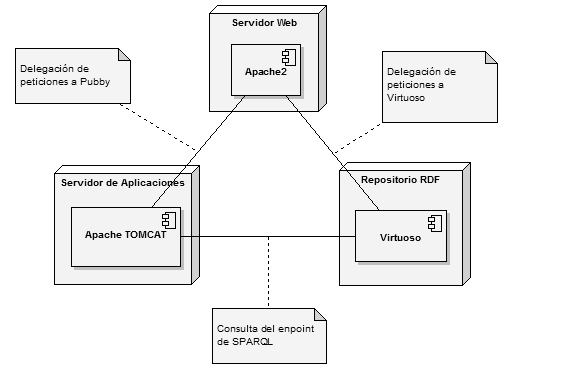
\includegraphics[width=10cm]{images/phd/infra-ld}
	\caption{Infraestructura Objetivo para \linkeddata.}
	\label{fig:infra-ld}
\end{figure}

Cada uno de estos componentes cumple una función específica que se detalla a continuación:
\begin{description}
 \item [Servidor web.] Teniendo presentes dos de los grandes objetivos de la publicación de datos enlazados como son el uso 
de HTTP URIs y que éstas sean en el mayor grado posible \textit{cool uris}, la presencia de un servidor web se justifica como punto 
de entrada a la consulta de los datos enlazados evitando la presencia de números de puerto, etc. y suministrando un acceso 
homogéneo a los datos. Para el cumplimiento de estos objetivos se ha seleccionado el servidor web Apache2. Por otra parte, con una configuración 
del servidor se da soporte al método de publicación basado en un ``\textit{Fichero estático RDF}''.
\item [Servidor de aplicaciones.] Este componente es el encargado de albergar las aplicaciones que proporcionan servicios de valor añadido 
de acceso a los datos desde diferentes puntos de vista. También se puede desplegar un contenedor de servlets que en muchos casos es suficiente. En este caso, 
seleccionando Pubby como elemento de software para dar soporte al método de publicación mediante un ``\linkeddata \textit{Frontend}''.
\item [Repositorio RDF.] Con el objetivo de albergar los datos transformados en RDF, es decir el \dataset RDF $\mathcal{D}$ es necesario el despliegue 
de un servidor RDF, para esta tarea existen diferentes opciones~\cite{5638466} pero Virtuoso de OpenLink se considera una buena opción por su amplia aceptación, 
capacidad de extensión y soporte a las especificaciones.
\item [\textit{Endpoint} de \gls{SPARQL}.] Del mismo modo que los datos transformados se han de almacenar también es conveniente proveer un interfaz de acceso 
a los mismos mediante el protocolo y lenguaje de consulta SPARQL. Igualmente existen diferentes opciones, sin embargo como parte de Virtuoso existe un módulo 
que se instala y está disponible automáticamente con el despliegue inicial del repositorio. El comportamiento de este componente se asemeja también a 
un servicio web \gls{REST} con peticiones GET facilitando de forma parcial otro método de publicación como el señalado en la Sección~\ref{servicio-web-produccion}.
\end{description}
% 
\subsubsection{Tarea $t_{15}$-Acceso y formato en datos RDF}\label{t15-comun}
Las necesidades de las aplicaciones para el posible consumo de datos varían ostensiblemente 
dependiendo de su objetivo. En el caso objeto de estudio de este documento y con la infraestructura 
indicada en la anterior sección se suministra soporte a los siguientes formatos de datos:

\begin{longtable}[c]{|p{4cm}|p{4cm}|p{4cm}|} 
\hline
  \textbf{Acceso} &  \textbf{Formato} &  \textbf{Provisto por}  \\\hline
\endhead
 Petición GET    & N3/Turtle    & Apache2 \\ \hline
 Consulta SPARQL & \textit{Spreadsheet}  & \textit{Endpoint} de SPARQL  \\ \hline
 $\equiv$        & XML 		& $\equiv$ \\ \hline
 $\equiv$        & JSON 	& $\equiv$ \\ \hline
 $\equiv$        & Javascript 	& $\equiv$  \\ \hline 
 Consulta SPARQL y petición GET      & N3/Turtle 	& \textit{Endpoint} de SPARQL y \linkeddata \textit{Frontend} \\ \hline
 $\equiv$        & RDF/XML 	& $\equiv$ \\ \hline
 $\equiv$        & NTriples 	& $\equiv$  \\ \hline
 $\equiv$        & HTML 	& $\equiv$  \\ \hline
 \hline
\caption{Acceso y Formato de datos de los Anuncios de Licitación.}\label{table:pscs-acceso}\\    
\end{longtable}

\subsection{Proceso de Consumo de Anuncios de Licitación}
El proceso de consumo de datos enlazados, según la definición realizada en la Sección~\ref{sect:proceso-consumo}, consiste en 
la reutilización de los datos enlazados para ser aplicados en la construcción de una nueva aplicación o servicio de valor 
añadido. En general, la reutilización más sencilla consiste en la representación gráfica de los recursos o la simple 
consulta con selección de formato de datos de acuerdo a las características de publicación utilizadas. En el caso 
que nos ocupa y teniendo en cuenta el objetivo de realización de un prototipo experimental de extracción de anuncios 
de licitación como demostrador del consumo de datos enlazados se ha escogido el método semántico de consumo $SCM_2$-``\textit{Mapeo} a Lenguaje de Programación'', 
cuya descripción está disponible en la Sección~\ref{scm2-consumo}, y orientado a obtener una representación de los recursos RDF en un 
lenguaje de programación (en este caso Java) como objetos de negocio. De acuerdo a este objetivo y la definición del propio método 
es necesario definir:
\begin{itemize}
 \item El \dataset RDF $\mathcal{D}_{pub}$, es el conjunto de datos disponible tras aplicar el método de publicación.
 \item El conjunto $\mathcal{M}^1$, ver Tabla~\ref{table:ppn-consumo}, indica como transformar el \dataset anterior a la representación objetivo, objetos del lenguaje Java.
\end{itemize}
% 
De esta manera, se obtiene una serie de objetos, $\mathcal{D}_{consum}$, con la información y datos necesarios, no se transforma necesariamente todos los datos disponibles en los recursos pertenecientes 
a  $\mathcal{D}_{pub}$, para ser reutilizados como objetos de negocio en un lenguaje de programación. Es conveniente señalar que el acceso a los datos se realiza a través 
de la consulta al \textit{endpoint} de \gls{SPARQL} realizando consultas \textit{SELECT} y \textit{DESCRIBE}.



\begin{longtable}[c]{|p{2cm}|p{6cm}|p{6cm}|} 
\hline
  \textbf{$\mathcal{M}^1$} &  \textbf{Propiedad} & \textbf{Tipo en Java} \\\hline
\endhead
 $m^1_1$ & URI recurso     		& \texttt{java.lang.String} \\ \hline
 $m^1_2$ & \texttt{rdf:type}      	& \texttt{org.weso.moldeas.to.PPNTO} \\ \hline
 $m^1_3$ & \texttt{dc:identifier} 	& \texttt{java.lang.String} \\ \hline
 $m^1_4$ & \texttt{dc:subject}    	& \texttt{java.lang.String} \\ \hline
 $m^1_5$ & \texttt{dc:date}    		& \texttt{java.util.Date} \\ \hline
 $m^1_6$ & \texttt{dc:publisher}	& \texttt{org.weso.moldeas.to.OrganizationTO} \\ \hline 
 $m^1_7$ & \texttt{ref-cpv} 		& \texttt{java.util.List<PSCTO> } \\ \hline
 $m^1_8$ & \texttt{ref-nuts} 		& \texttt{java.util.List<NUTSTO> }\\ \hline
 $m^1_9$ & \texttt{foaf:topic} 	& \texttt{java.util.List<PSCTO> } \\ \hline
 $m^1_{10}$ &  \texttt{rdfs:label}  & Map<String,String> (lang, value) para cada propiedad \\ \hline   
 $m^1_{11}$ &  \texttt{rdfs:description}  & Map<String,String> (lang, value) para cada propiedad \\ \hline   
  \multicolumn{3}{|c|}{\ldots} \\ \hline
\hline
\caption{Conjunto de \textit{mapeos} $\mathcal{M}^1$ de consumo para los Anuncios de Licitación.}\label{table:ppn-consumo}\\    
\end{longtable}

\subsection{Proceso de Validación de Anuncios de Licitación}
La validación como proceso transversal a cualquier etapa dentro del ciclo de vida de datos 
enlazados debe realizarse con el objetivo de asegurar la calidad de los datos. De acuerdo a la 
definición realizada en la Sección~\ref{sect:validation}, este proceso consiste en la comprobación 
de que los recursos de un \dataset RDF cumplen ciertas características. La realización de esta validación 
puede ser realizada manual o automáticamente dependiendo del caso, por ejemplo para la características 
de negociación de contenido se dispone de herramientas o para la inclusión en la nube de datos enlazados, pero 
en cambio para comprobaciones relativas a los dominios y rangos de las propiedades, etc., no existe una 
herramienta completo. Por todo ello, se ha seguido un enfoque híbrido basado en la utilización de herramientas 
y validación manual. La descripción completa de la validación de acuerdo a todas las características 
se reseña en las Tablas de Validación disponibles en el Apéndice~\ref{tablas-validacion-apen}.
% 
\subsubsection{Tarea $t_{12}$-Validación de Recursos RDF}
Siguiendo con la definición realizada de esta tarea en la Sección~\ref{lod-t12}, se puede asegurar que la transformación 
realizada de los anuncios de licitación a la iniciativa \linkeddata cumple estrictamente los 
siguientes puntos:

\begin{itemize}
 \item Los datos RDF correctos ya que se han utilizado herramientas y APIs (Google Refine y Jena) que aseguran 
la generación correcta de RDF.
 \item El dominio y rango en las propiedades es correcta a realizar la validación contra el modelo definido.
 \item Se ha establecido metainformación sobre la procedencia a nivel de \dataset.
 \item Todos los recursos transformados siguen la plantilla objetivo RDF.
\end{itemize}
% 
En conclusión, las tareas, métodos y el proceso de validación tienen un calado verdaderamente trascendente 
en el ciclo de vida de datos enlazados, es por ello que en este estudio se ha rendido especial interés 
a la consecución correcta de la validación de los datos enlazados.
% 
\subsection{Proceso de Realimentación de Anuncios de Licitación}
Este proceso según la definición realizada en la Sección~\ref{proceso-realimentacion} busca la mejora 
y perfeccionamiento de los datos promocionados a \gls{RDF}. Esta situación emerge en el momento en el cual 
los datos comienzan a ser reutilizados tanto por aplicaciones o servicios como por individuos. En el caso 
particular de los anuncios de licitación no se ha llegado a ser reutilizados por terceras partes, 
por lo que la realimentación ha quedado restringida a la captura de fallos por la propia aplicación \gls{MOLDEAS}, 
tratándose en este caso de una forma de realimentación basada en \textit{Usuarios y Aplicaciones} 
y de carácter \textit{Actualización Ocasional}.



\section{Clasificaciones Estándar de Productos}
Los sistemas de organización del conocimiento, \textit{Knowledge Organization Systems} (\gls{KOS}), como
tesauros, taxonomías o sistemas de clasificación, se han desarrollado en el seno de distintas comunidades e instituciones, 
principalmente con el objetivo de organizar grandes bases de datos que contienen recursos de diferente tipo tales como documentos, 
páginas web o elementos multimedia. Estos vocabularios permiten a los usuarios la anotación
de los objetos de información de los recursos para simplificar su extracción y consulta, habitualmente 
se utilizan técnicas de indexado por un determinado tema con el objeto de facilitar el acceso también para las máquinas, 
suministrando los metadatos necesarios en la descripción de los objetos de información.

En el dominio de la contratación pública electrónica estas clasificaciones resultan de gran 
interés para la especificación de los objetos de contrato, así como para la extracción de 
%estadísticas a posteriori. Como se ha reseñado en la Sección~\ref{sect:pscs}, una de las
estadísticas a posteriori. Como se ha reseñado en los entregables \textit{AEN01-00 y AEN01-01}, una de las 
principales clasificaciones en este sentido es el ``\textit{Common Procurement Vocabulary}''(\gls{CPV})~\cite{cpvguide}, 
pero también existen otros esquemas de clasificación de gran interés en la esfera del comercio 
electrónico, así la ``\textit{Combined Nomenclature}'' o el ``\textit{North American Product Classification System}''. 
En el ámbito de esta tesis se ha optado por promocionar las clasificaciones más importantes en este contexto 
para facilitar el acceso a los anuncios de licitación independientemente de la clasificación utilizada, para ello, 
se ha realizado la transformación siguiendo los principios de \linkeddata y los métodos definidos en el capítulo anterior de 
las siguientes clasificaciones estándar de productos (\gls{PSC}s) (un total de $9$), ver Tabla~\ref{table:pscs-ld}.

\begin{longtable}[c]{|p{6cm}|l|p{6cm}|} 
\hline
  \textbf{Clasificación} &  \textbf{Acrónimo} & \textbf{Organismo} \\\hline
\endhead
\textit{Common Procurement Vocabulary}, (2003 y 2008) & \gls{CPV} & Unión Europea \\ \hline
\textit{Combined Nomenclature} 2012 (desde 1995) & \gls{CN} & Unión Europea  \\ \hline
\textit{Central Product Classification}, version 2 (2008) & \gls{CPC} & Unión Europea \\ \hline
Clasificación de Productos por Actividad (2008) & \gls{CPA} & Unión Europea \\ \hline
\textit{International Standard Industrial Classification of All Economic Activities, Rev.4} & \gls{ISIC} & \textit{United Nations Statistics Division} \\ \hline
\textit{North American Industry Classification System} 2007 y 2012 & \gls{NAICS} & Gobierno de Estados Unidos \\ \hline
\textit{Standard International Trade Classification, Revision 4} & \gls{SITC} & \textit{United Nations Statistics Division} \\ \hline
%\textit{Nomenclature générale des activités économiques dans les Communautés européennes} & NACE & Unión Europea \\ \hline
\hline
\caption{Catálogo de Clasificaciones Estándar de Productos seleccionadas.}\label{table:pscs-ld}\\    
\end{longtable}

\subsection{Proceso de Producción de \linkeddata de Clasificaciones\\ Estándar de Productos}
Siguiendo la definición realizada en la Sección~\ref{sect:produccion}, este proceso conlleva
todas las tareas que implican la transformación de un \dataset de entrada $\mathcal{G}$, mediante
unas reglas de \textit{mapeo} $\mathcal{M}$, para la obtención de un \dataset \gls{RDF} $\mathcal{D}$, método semántico 
de producción. 

\subsubsection{Tarea $t_1$-Análisis del \dataset a transformar}\label{t1-pscs}
Las \gls{PSC}s como instrumentos claves de estandarización nacen con el fin de
conseguir una clasificación común de productos y servicios. Las diferencias entre las clasificaciones no
sólo se limitan a cuestiones de alcance y cobertura sectorial de producto, sino también al grado de especificidad que difiere de unas a otras.

%%Como ya se ha reseñado en la Sección~\ref{semantica:pscs}, Hepp~\cite{HeppTrueComplexity,HeppEclass,HeppMethodology} apunta
Como ya se ha reseñado en los entregables \textit{AEN01-00 y AEN01-01}, Hepp~\cite{HeppTrueComplexity,HeppEclass,HeppMethodology} apunta
a estos estándares como una combinación de componentes variables que pueden ser utilizados 
para la construcción de ontologías derivadas, sin embargo, se puede identificar 
una estructura común subyacente a todas las PSCs y que debe considerarse fundamental para 
proporcionar un modelo de datos semántico universal para las PSCs, para ello, se utilizarán 
los conceptos los conceptos de \textit{árbol} y \textit{bosque} provenientes de la teoría de 
grafos con el objetivo de representar la estructura común de las PSCs. 

\begin{description}
 \item [Categorías de productos.] Las clasificaciones se dividen en categorías o
clases de productos. Estas categorías agrupan los distintos elementos de la PSC,
$Cat_{psc}$, en distintos niveles de especialización semántica o niveles de
jerarquía: $Cat_{psc} = \displaystyle\bigcup_{n=0}^k{(Cat_{psc}^n)}$, desde
términos genéricos, como el caso del elemento del \gls{CPV}-``Servicios de reparación y mantenimiento'' (código 50000000), hasta productos altamente
específicos y directamente identificables, como en un elemento de la misma jerarquía anterior pero con un mayor nivel 
de especificidad como ``Servicios de reparación y mantenimiento de instalaciones contra incendios'' (código 50413200). Una PSC cumple las siguientes
características:
\begin{itemize}
 \item Las categorías de la PSC se organizan jerárquicamente: $Cat_{psc}^0\succ
Cat_{psc}^1\succ...\succ Cat_{psc}^n $.
 \item Cada elemento de la PSC, $t_{psc}^x$, pertenece a una categoría de
productos.
 \item Cada elemento de la PSC, $t_{psc}^x$, pertenece sólo a una categoría de
productos. Es decir, las categorías son disjuntas:
$\displaystyle\bigcap_{n=0}^k{(Cat_{psc}^n)}=\emptyset$.
\end{itemize}


\item  [Estructura taxonómica.] Además de la división en niveles de jerarquía
de los elementos de una \gls{PSC}, su objetivo es organizar y agrupar los productos en
sectores verticales mediante algún tipo de criterio establecido por la comunidad
que desarrolla el estándar. Formalmente, esta estructura taxonómica de cada
sector de productos tiene forma de árbol, $T_{psc}$: todos los elementos
$t_{psc}^n$ tienen un elemento de nivel superior $t_{psc}^{n-1}$. Además el
conjunto de sectores de productos de una clasificación constituye la propia PSC,
que puede definirse como un \textbf{bosque} ($\mathbb{F}_{psc}$) de árboles
($T_{psc}$), en el que se cumple que:
\begin{itemize}
 \item $\mathbb{F}_{psc}= \displaystyle\bigcup_{m=0}^k{(T_{psc}^m)}$
 \item Cada elemento $t_{psc}^0$ es la \textbf{raíz} de una agrupación de
productos estructurada jerárquicamente en forma de árbol, $T_{psc}^x$.
 \item Cada elemento $t_{psc}$ pertenece a uno de estos árboles de productos
$T_{psc}^x$.
 \item Por la propia definición de bosque, cada elemento $t_{psc}$ pertenece sólo
a un $T_{psc}^x$. Es decir, cada sector de productos es disjunto:
$\displaystyle\bigcap_{m=0}^k{(T_{psc}^m)}=\emptyset$.
\end{itemize}
 
\end{description}

Estas son características genéricas de las clasificaciones de productos, sin
embargo, otras PSCs más sofisticadas incluyen un diccionario de propiedades
estándar que se puede utilizar para describir productos con más detalle.
Normalmente, estos diccionarios de propiedades también incluyen los tipos de
datos que pueden ser valor de las mismas, así como su referencia con respecto
a estándares internacionales para establecer las unidades de medida, tal es el caso
de la clasificación de productos de e@Class. En otras ocasiones, se construyen
clasificaciones multiling\"{u}es para la expresión de los descriptores de cada
elemento de la PSC, el caso extremo es el \gls{CPV}, donde se contempla un total de hasta $23$ lenguas.

El desafío básico más importante que hay que afrontar cuando se deriva una
ontología de una PSC, reside en cómo interpretar la semántica original de la taxonomía.
No existe una definición formal de las relaciones taxonómicas que construyen
cada $T_{psc}$ de la clasificación y es tentador utilizar la propiedad de un
vocabulario de ontologías, como \textit{rdfs:subClassOf}, para intentar
representar estas relaciones semánticas. La postura del enfoque seguido es 
%%radicalmente distinta, ver Sección~\ref{semantica:pscs}, desde este punto de vista, las PSCs fueron construidas
radicalmente distinta, ver entregables \textit{AEN01-00 y AEN01-01}, desde este punto de vista, las PSCs fueron construidas 
para solucionar problemas de comunicación, proporcionar una
forma de organizar tipos de productos y agruparlos de acuerdo a unos conceptos y
definiciones que funcionasen \textit{de facto} como un estándar en determinados
entornos de actividad comercial e industrial. Las PSCs no fueron diseñadas como
modelos conceptuales de dominio, en el sentido actual que tiene el término
``ontología'', sino como una forma de estructurar la terminología y la forma de
nombrar los productos, de ahí que se interpreten las PSCs como simples
esquemas conceptuales en el que la relación taxonómica que jerarquiza los
distintos elementos de cada $T_{psc}$ no se interpreta como una relación de
herencia o subtipo, sino como una relación de mayor o menor especificidad de los
elementos. Resumiendo, se consideran las PSCs como simples vocabularios
controlados y se utilizará una ontología RDF/\gls{OWL}, \gls{SKOS} Core, como modelo de
datos común.

La adopción de una ontología como SKOS Core para modelar las PSCs está
completamente justificada desde este enfoque, se trata de una ontología RDF/OWL que gira en torno a dos clases principales
\textit{skos:Concept} y \textit{skos:ConceptScheme}, así todos los elementos de una
PSC son considerados instancias de \textit{skos:Concept}, de manera que se
entiende que todos ellos son conceptualizaciones de recursos. Asumiendo este
modelo, la interpretación de cada elemento $t_{psc}$ de una PSC es natural, directa y no provoca incoherencias en su 
tratamiento, tal como se ha reseñado en los ejemplos anteriores de inconsistencia. El interés de este enfoque, radica en la posibilidad de poder 
replicar completamente la semántica original de las PSCs.

Para agrupar todos los elementos de una \gls{PSC} bajo un paraguas común, se construye una
clase contenedora de todos los $t_{psc}$: $PSCConcept$, declarándola como
subclase del concepto $skos:Concept$: 

\begin{equation}
 PSCConcept \sqsubseteq skos:Concept
\end{equation}

Esta clase a su vez se puede dividir en distintas categorías que constituyen
los niveles de jerarquía del PSC (si los hubiera). El atractivo en la utilización de SKOS Core reside 
en que es factible replicar completamente el modelo de datos común de las PSCs, de esta forma, por cada $Cat_{psc}^k$,
se construye un concepto subclase de \textit{PSCConcept}, en el caso particular del \gls{CPV}:

\begin{equation}
 Division \sqsubseteq PCSConcept;Grupo \text{...}
\end{equation}

Y se mantiene la semántica original de la clasificación añadiendo los siguientes
axiomas, perfectamente expresables en OWL-DL para el caso del CPV. En otras clasificaciones, no 
es posible establecer este tipo de axiomas debido a la falta de designación de categorías ya que la 
relación de jerarquía se establece simplemente mediante un código numérico.

\begin{equation}
 PSCConcept\ \equiv Division\ \sqcup\ Grupo \sqcup\ Clase\ \sqcup\ Categoria
\end{equation}

\begin{equation}
Division \sqcap\ Grupo \sqcap\ Clase\ \sqcap\ Categoria = \perp
\end{equation}

Por otro lado, el segundo factor importante a destacar reside en la estructura taxonómica de cada
$T_{psc}$, que como se ha referido, tenía una difícil interpretación como conjunto de
relaciones de herencia clásica, sin embargo, bajo el paradigma SKOS Core se contemplan relaciones 
semánticas tales como: \texttt{skos:inScheme}, \texttt{skos:related}, \texttt{skos:broader}, \texttt{skos:narrower} y sus versiones transitivas, que
constituyen el marco conceptual adecuado para el establecimiento de las relaciones entre los elementos de la PSC.

Finalmente, la clase \textit{skos:ConceptScheme} deviene necesario para completar la 
interpretación de una PSC y su modelo, ver Figura~\ref{fig:modelo-grafico-pscs}, se reifica 
una PSC como una instancia de esta clase para también así contextualizar los 
términos y distinguirlos e identificarlos en lo referido a un entorno web.

\begin{equation}
 PSCConcept \equiv\ni inScheme~PSCScheme
\end{equation}


\begin{figure}[!htp]
 \centering
	 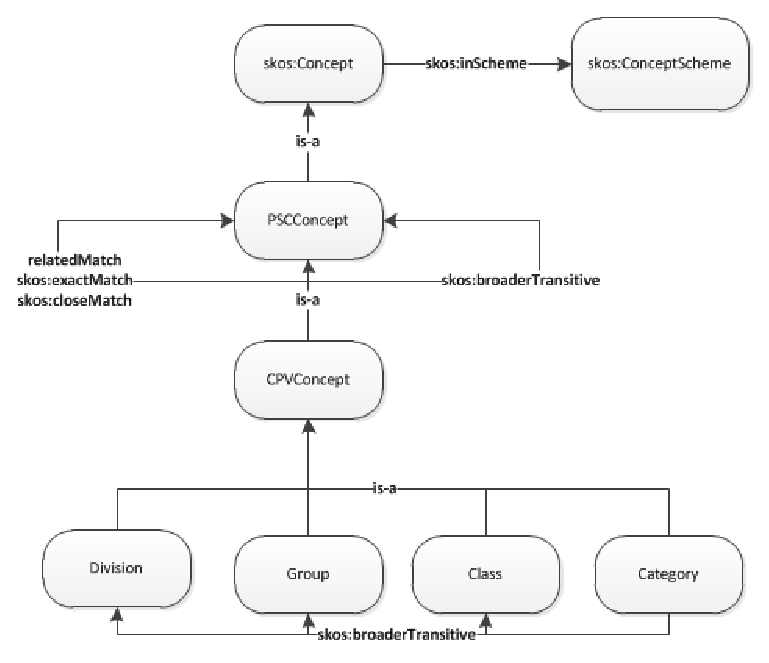
\includegraphics[width=10cm]{images/phd/modelo/pscs-model}
	\caption{Modelo gráfico para las Clasificaciones Estándar de Productos.}
	\label{fig:modelo-grafico-pscs}
\end{figure}



\subsubsection{Tarea $t_2$-Limpieza de datos}
Los datos provenientes de las clasificaciones de productos se encuentran disponibles, en la mayoría de los casos, 
en hojas de cálculo MSExcel o bien directamente en formato \gls{CSV} en los cuales ya se ha realizado un esfuerzo por los organismos 
creadores para evitar caracteres extraños o incorrectos. Habitualmente, todos estos datos provienen de fuentes oficiales por lo que
este proceso ya ha sido realizado en la labor de creación de los mismos, es por lo que en la promoción de estos datos, esta tarea
ya ha sido realizada y no es necesario aplicar ningún filtro especial a los datos ya disponibles. Esta circunstancia supone 
un gran avance para la transformación de datos, ya que se dispone de aquellos clasificados con $2\star$ según los principios de \linkeddata y no 
es necesario realizar procesos de \textit{screen-scrapping} con la consiguiente ganancia en la calidad de los datos.

\subsubsection{Tarea $t_3$-Selección de Vocabularios}
Los vocabularios seleccionados para modelar las clasificaciones de productos, teniendo en cuenta el análisis 
realizado en la tarea $t_1$ se presentan en la Tabla~\ref{table:pscs-select-vocabs}. En general, se trata de vocabularios 
que atienden a los siguientes criterios:

\begin{enumerate}
 \item Formalización de una estructura taxonómica, como RDFS, \gls{SKOS} u \gls{OWL}.
 \item Realización de \textit{mapeos} entre conceptos, como SKOS y OWL.
 \item Representación de tipos de datos, como \gls{XML Schema}.
 \item Gestión de información multiling\"{u}e, como \gls{SKOS-XL} y RDFS.
 \item Representación de información de negocio, como \textit{GoodRelations} y \textit{ProductOntology}.
 \item Adición de metadatos y \textit{provenance}, como \textit{Dublin Core Terms}, \gls{voID} y \textit{Provenance Ontology}.
 \item Representación del tiempo e intervalos, como \textit{Time Ontology} del \gls{W3C}.
\end{enumerate}


\begin{longtable}[c]{|l|p{4cm}|p{4cm}|p{4cm}|} 
\hline
\textbf{Prefijo} &  \textbf{Vocabulario} &  \textbf{Fuente} & \textbf{Uso} \\\hline
\endhead
 dbpedia & \url{http://dbpedia.org/ontology/}&  Comunidad \linkeddata. & Reutilización de definiciones. \\ \hline 
 dc & \url{http://purl.org/dc/elements/1.1/}&  \textit{Dublin Core Metadata Initiative} & Creación de metadatos para los documentos. \\ \hline  
 dct & \url{http://dublincore.org/documents/dcmi-terms/}&  $\equiv$ & $\equiv$ \\ \hline  
 foaf & \url{http://xmlns.com/foaf/0.1/} &Comunidad de Web Semántica.& Especificación de relaciones entre personas. \\ \hline 
 gr & \url{http://purl.org/goodrelations/v1#} & Martin Heep & Reutilización de definiciones para describir productos y servicios.\\\hline 
 owl  & \url{http://www.w3.org/2002/07/owl#} & W3C & Realización de definiciones en el dominio. \\\hline
 po & \url{http://www.productontology.org/} & \textit{Martin Heep} & Reutilización de datos provenientes de Productontology.\\\hline 
 skos & \url{http://www.w3.org/2004/02/skos/core#} & W3C & Especificación de taxonomías. \\ \hline
 skosxl & \url{http://www.w3.org/2008/05/skos-xl#>} & W3C & Representación de información ling\"uística. \\ \hline
 rdf & \url{http://www.w3.org/1999/02/22-rdf-syntax-ns#} & W3C & Descripción de recursos. \\ \hline
 rdfs & \url{http://www.w3.org/2000/01/rdf-schema#} & W3C & Descripción de recursos con relaciones lógicas. \\ \hline 
 void & \url{http://rdfs.org/ns/void#} & Deri y W3C & Descripción de metadatos de un \dataset. \\\hline
 xml & \url{http://www.w3.org/XML/1998/namespace} & W3C & Reutilización de definiciones. \\\hline
 xsd & \url{http://www.w3.org/2001/XMLSchema#} & W3C & Especificación de tipos de datos. \\\hline
\hline
\caption{Selección de Vocabularios para las Clasificaciones Estándar de Productos.}\label{table:pscs-select-vocabs}\\    
\end{longtable}

\subsubsection{Tarea $t_4$-Selección de otros \datasets RDF}
Al igual que en la sección anterior, los \datasets a reutilizar se centran en vocabularios de negocio 
ya existentes y por consiguiente en los datos disponibles en los mismos, de esta forma, se reutilizan 
y enlazan datos provenientes de \textit{GoodRelations} y \textit{ProductOntology}, ver Tabla~\ref{table:pscs-select-datasets}.

\begin{longtable}[c]{|l|p{4cm}|p{4cm}|p{4cm}|} 
\hline
  \textbf{Prefijo} &  \textbf{\textit{Dataset}} &  \textbf{Fuente} & \textbf{Uso} \\\hline
\endhead
dbpedia-res & \url{http://dbpedia.org/}&  Comunidad \linkeddata. & Reutilización de datos provenientes de la DBPedia. \\ \hline 
gr & \url{http://purl.org/goodrelations/v1#} & \textit{Martin Heep} & Reutilización de definiciones para describir productos y servicios.\\\hline 
po & \url{http://www.productontology.org/} & \textit{Martin Heep} & Reutilización de datos provenientes de ProductOntology.\\\hline 
\hline
\caption{Selección de otros \datasets para las Clasificaciones Estándar de Productos.}\label{table:pscs-select-datasets}\\    
\end{longtable}


\subsubsection{Tarea $t_5$-Modelado de datos en RDF}\label{sect:pscs-data-model}
El resultado de esta tarea debe ser una ontología de dominio $\mathcal{O}$. que modele los recursos $t_{psc}$, pertenecientes a un 
\dataset RDF $\mathcal{D}$. Inicialmente, se debe proveer la especificación del modelo 
formal u ontología $\mathcal{O}$ de acuerdo al análisis realizado en la Sección~\ref{t1-pscs}, dando soporte 
a la descripción de los datos de los recursos \gls{RDF}:

\begin{itemize}
 \item $\mathcal{C} = \{$\textit{PSCConcept, CPVConcept, Division, Group, Class, Category}$\}$
 \item $\mathcal{R} = \{$\textit{rdf:type, skos:inScheme, dc:identifier, dc:subject, level, pscs:relatedMatch, pscs:level, skos:exactMatch, skos:broaderTransitive, skos:prefLabel, rdfs:label, gr:description}$\}$
 \item $\mathcal{I} = \{ t_{psc} \}$
 \item $\mathcal{A} = \{\star\}$, son los axiomas propios de una ontología en SKOS.
\end{itemize}
 
Como segundo paso se diseñan las propiedades que deben tener los recursos, teniendo en cuenta su ulterior aplicación, 
ver Tabla~\ref{table:pscs-rdf-model}, pertenecientes a ese \dataset, comunes para todas las \gls{PSC}s.

Una vez especificado el conjunto de propiedades de cada elemento $t_{psc}$ es necesario definir el conjunto 
de grafos en los cuales se encuadrarán los recursos, es decir, el \dataset \gls{RDF} $\mathcal{D}$. Para ello, 
en la Tabla~\ref{table:pscs-dataset} se indican las tuplas $(\mathcal{G}_k, I_k)$ correspondientes a cada uno 
de los grafos $\mathcal{G}_k$ identificados a través de la URI $I_k$.

\begin{longtable}[c]{|p{3cm}|p{9cm}|} 
\hline
  \textbf{$\mathcal{G}_k$} &  \textbf{$I_k$}  \\\hline
\endhead
 \textbf{$\mathcal{G}$}   & \url{http://purl.org/weso/pscs} \\ \hline
 \textbf{$\mathcal{G}_1$} & \url{http://purl.org/weso/pscs/cpv/2008} \\ \hline
 \textbf{$\mathcal{G}_2$} & \url{http://purl.org/weso/pscs/cpv/2003} \\ \hline
 \textbf{$\mathcal{G}_3$} & \url{http://purl.org/weso/pscs/cn/2012} \\ \hline
 \textbf{$\mathcal{G}_4$} & \url{http://purl.org/weso/pscs/cpc/2008} \\ \hline
 \textbf{$\mathcal{G}_5$} & \url{http://purl.org/weso/pscs/cpa/2008} \\ \hline
 \textbf{$\mathcal{G}_6$} & \url{http://purl.org/weso/pscs/isic/v4} \\ \hline
 \textbf{$\mathcal{G}_7$} & \url{http://purl.org/weso/pscs/naics/2007} \\ \hline
 \textbf{$\mathcal{G}_8$} & \url{http://purl.org/weso/pscs/naics/2012} \\ \hline
 \textbf{$\mathcal{G}_9$} & \url{http://purl.org/weso/pscs/sitc/v4} \\ \hline
 \textbf{$\mathcal{G}_{10}$} & \url{http://purl.org/weso/pscs/ontology} \\ \hline 
\hline
\caption{\textit{Dataset} RDF $\mathcal{D}$ para Clasificaciones Estándar de Productos.}\label{table:pscs-dataset}\\    
\end{longtable}


\begin{longtable}[c]{|p{5cm}|p{4.5cm}|p{5cm}|} 
\hline
  \textbf{Propiedad} &  \textbf{Descripción} & \textbf{Ejemplo} \\\hline
  \texttt{rdf:type} & Especificación del tipo de un recurso $t_{psc}$ & a \texttt{gr:ProductOr ServiceModel}, \texttt{PSCConcept} \\ \hline
  \texttt{skos:inScheme} & \gls{URI} al esquema de la PSC $T_{psc}$ a la que pertenece $t_{psc}$ & \texttt{skos:inScheme} cpv2008:ds \\ \hline
  \texttt{dc:identifier} & Identificador utilizado en la URI del recurso $t_{psc}$ &  \texttt{dc:identifier} "55900000"$\textasciicircum\textasciicircum$xsd:string \\ \hline
  \texttt{dc:subject} & Identificador original proveniente de la fuente de datos &  \texttt{dc:subject} "55900000-9"$\textasciicircum\textasciicircum$xsd:string \\ \hline
  \texttt{pscs:relatedMatch} & URI a un recurso $t'_{psc}$ que encaja parcialmente con $t_{psc}$ & \texttt{po:retail} \\ \hline
  \texttt{skos:exactMatch } & URI a un recurso $t'_{psc}$ que encaja totalmente con $t_{psc}$ & \texttt{cpv2008:52900000} \\ \hline
  \texttt{skos:closeMatch } & URI a un recurso $t'_{psc}$ del CPV 2008 que encaja parcialmente con $t_{psc}$ & \texttt{cpv2008:52900000} \\ \hline
  \texttt{pscs:level} & Indica el grado de especificidad de un $t_{psc}$ cuando no se puede inferir directamente su antecesor & \texttt{pscs:level} ``5'' \\ \hline  
  \texttt{skos:broaderTransitive} & URI a un recurso $t'_{psc}$ antecesor de $t_{psc}$ que indica la categoría $Cat_{psc}$ & \texttt{skos:broaderTransitive} cpv2008:55000000 \\ \hline
  \texttt{skos:prefLabel} & Etiquetas y descripciones multing\"{u}es &  "Retail trade services"@EN \\ \hline
  \texttt{rdfs:label} & $\equiv$ &  $\equiv$\\ \hline
  \texttt{gr:description} & $\equiv$ &  $\equiv$ \\ \hline
\endhead
\hline
\caption{Diseño de propiedades para los elementos de las Clasificaciones Estándar de Productos.}\label{table:pscs-rdf-model}\\    
\end{longtable}




\subsubsection{Tarea $t_6$-Diseño de un Esquema de URIs}
Esta tarea tiene como objetivo establecer la forma y estructura de las \gls{URI}s tanto para las definiciones 
realizadas en la ontología $\mathcal{O}$ como para todos los recursos presentes en el \dataset RDF $\mathcal{D}$ que 
se genera a partir de la transformación de los datos a \gls{RDF}. Es una de las actividades clave ya que guiará 
tanto el método final de transformación como el proceso posterior de publicación. En la Tabla~\ref{table:pscs-uris} se 
hace la descripción de la estructura de URIs que se seguirán para las \gls{PSC}s.

\begin{longtable}[c]{|p{5cm}|p{4.5cm}|p{5cm}|} 
\hline
  \textbf{URI} &  \textbf{Descripción} & \textbf{Ejemplo} \\\hline
\endhead
\url{http://purl.org/weso/pscs/} & URI base: <base\_uri> & NA \\ \hline
\url{<base_uri>/ontology} & Definiciones comunes a todas las PSC & \url{<base_uri>/ontology/PSCConcept} \\ \hline
\url{<base_uri>/resource/ds} & Descripción del catálogo de las PSCs & \url{<base_uri>/resource/ds} \\ \hline
\url{<base_uri>/{psc}/{version|year}} & Espacio de nombres para una determinada PSC & \url{<base_uri>/cpv/2008} \\ \hline
\url{<base_uri>/{psc}/{version|year}/ontology} & Definiciones particulares de una PSC & \url{<base_uri>/cpv/2008/ontology} \\ \hline
\url{<base_uri>/resource/{psc}/{version|year}/{id}} & URI para un recurso de una PSC & \url{<base_uri>/cpv/2008/resource/55900000} \\ \hline
\url{<base_uri>/resource/{psc}/{version|year}/ds} & URI la descripción del \dataset de una PSC & \url{<base_uri>/cpv/2008/resource/ds} \\ \hline
\hline
\caption{Diseño de URIs para las Clasificaciones Estándar de Productos.}\label{table:pscs-uris}\\    
\end{longtable}

\subsubsection{Tarea $t_7$-Diseño Plantilla Objetivo del Recurso RDF}
El objetivo de esta tarea es establecer una plantilla de cada uno de los recursos RDF que están 
presentes en el \dataset \gls{RDF} $\mathcal{D}$ para que sirvan como guía en los siguientes momentos: 1) en la ejecución propiamente dicha 
de la transformación de los datos originales a RDF y 2) en la validación de los recursos RDF generados. De esta manera, 
tratándose de \datasets con una gran cantidad de recursos se pueden identificar fácilmente aquellos que no sean 
compatibles con este esquema favoreciendo la depuración de los recursos generados. Adicionalmente, un esquema de 
recurso sirve como documentación extra para el proceso de consumo. En el caso de las clasificaciones de productos es necesario 
establecer un recurso plantilla, ver Figura~\ref{fig:pscs-template}, para los propios elementos de la \gls{PSC}, $t_{psc}$, así como para la propia descripción 
de los \datasets. No obstante, esta descripción se delega a la tarea $t_{16}$-``Añadir metainformación a los recursos RDF'', 
ver Sección~\ref{t16-pscs}.

De acuerdo al recurso plantilla y a las definiciones realizadas en la ontología que modela estos datos 
es posible realizar una validación en cuanto a los tipos de datos, cardinalidad de las relaciones, tipo de objetos, etc., que 
resulta de sumo interés para asegurar la calidad de los datos producidos.

\begin{figure}[!htp]
\begin{lstlisting} 
<<base_uri>/resource/{psc}/{version|year}/{id}>
      a       gr:ProductOrServiceModel , pscs:PSCConcept;
     (skos:prefLabel ""@lang;)+
     (gr:description ""@lang;)+
     (rdfs:label ""@lang ;)+
     dc:identifier ""^^xsd:string ;
     dc:subject ""^^xsd:string ;
     (pscs:relatedMatch <uri>;)*
     (pscs:level <uri>;)*
     (skos:broaderTransitive <uri>;)[0,1]
     (skos:exactMatch <uri>; )*
     skos:inScheme <<base_uri>/resource/{psc}/{version|year}/ds> .	
\end{lstlisting}
	\caption{Plantilla Objetivo de un Recurso de las Clasificaciones Estándar de Productos.}
	\label{fig:pscs-template}
\end{figure}



\subsubsection{Tarea $t_8$-Enriquecimiento de los datos en RDF}\label{t8-pscs}
El objetivo de esta tarea es enlazar los recursos generados del \dataset RDF $\mathcal{D}$ con otros 
ya existentes. En el caso particular de las clasificaciones de productos y de acuerdo a los \datasets 
identificados en la Tarea $t_4$, el enriquecimiento de los elementos se realizará con \textit{ProductOntology} que 
a su vez dispone de enlaces a la DBPedia, con lo que el enlazado de los datos queda perfectamente justificado. 

Para llevar a cabo el enriquecimiento es necesario realizar reconciliación de entidades entre las descripciones 
de elementos $t_{psc}$ y los recursos objetivos. Análogamente a enfoques como los de \textit{Silk Server} o SERIMI y teniendo 
en cuenta las particularidades de las descripciones de los productos se ha decido implementar un componente, 
como parte de \texttt{moldeas-transformer}, para realizar este enlazado, tomando como entrada la descripción del producto, en inglés, y tras 
la realización del procesamiento de lenguaje natural mediante las herramientas Apache \gls{Lucene}~\cite{Hatcher:2004:LA:1044938} y \gls{Solr}~\cite{solr}, obtiene una lista de recursos 
candidatos a ser enlazados. Dado que el \textit{matching} de los recursos no se puede asegurar al 100\%, requeriría una validación manual, 
por lo que se ha creado una propiedad particular \textit{pscs:relatedMatch} para indicar la relación que se establece entre el recurso 
actual $t_{psc}$ y el recurso obtenido. Adicionalmente, en una segunda versión se ha especializado esta propiedad para incluir 
un valor de fiabilidad (\textit{threshold}) que indica el grado de similitud entre los recursos, de esta manera se pueden obtener 
los recursos similares a uno dado por encima de un valor umbral.

Por otra parte, en el ámbito de los anuncios de licitación la clasificación de productos más relevante es el \gls{CPV} 2008 ya que 
es el sistema de clasificación vigente y normativo en la Unión Europea. Teniendo en cuenta que los anuncios de licitación 
objeto de estudio en este documento pertenecen a la Unión Europea y que por lo tanto están clasificados de acuerdo a esta 
taxonomía, es conveniente proveer los enlaces adecuados entre los distintos elementos de todas las PSCs para que puedan 
ser traducidos al CPV 2008 facilitando la capacidad expresiva para la realización de consultas y en consecuencia favoreciendo 
la accesibilidad a los anuncios de licitación. El soporte a este enfoque sigue un modelo similar al presentado anteriormente, 
con la diferencia de que los recursos origen son aquellos generados en la transformación de las \gls{PSC}s y el \dataset objetivo 
es el correspondiente al CPV 2008. De esta manera, se establecen dos tipos de enlaces:
\begin{enumerate}
 \item \textit{Mapping} exacto. Este enlace entre elementos de las PSCs se realiza cuando en las propias clasificaciones existen 
\textit{mapeos} entre los elementos porque un organismo oficial se ha encargado de realizar esta tarea por cuestiones estratégicas. En este caso, 
el enlace entre los conceptos se modela mediante la propiedad \texttt{skos:exactMatch} cuya semántica dentro de la especificación 
de SKOS indica que su uso estará destinado a realizar enlaces entre conceptos \textit{skos:Concept}, en los cuales se puede asegurar 
que representan al mismo recurso.
\item \textit{Mapping} parcial. Al igual que en el caso anterior el proceso consiste en identificar los recursos del CPV 2008 que encajan 
parcialmente con un recurso origen en otra PSC. En este caso, la propiedad utilizada es \texttt{skos:closeMatch} que de acuerdo 
a su semántica permite establecer enlaces entre conceptos \textit{skos:Concept}. Igualmente, se ha especializado este caso 
para contener un valor umbral del enlace.
\end{enumerate}
 
En conclusión, la ejecución de esta tarea permite por un lado crear enlaces entre todas las PSCs y un \dataset externo y por otra parte, 
crear enlaces entre todas las PSCs y el CPV 2008. El enriquecimiento realizado en las PSCs conduce finalmente a la siguiente estructura, 
ver Figura~\ref{fig:linked-pscs}, de enlaces entre las distintas PSCs y los \datasets externos.

\begin{figure}[!htb]
\centering
	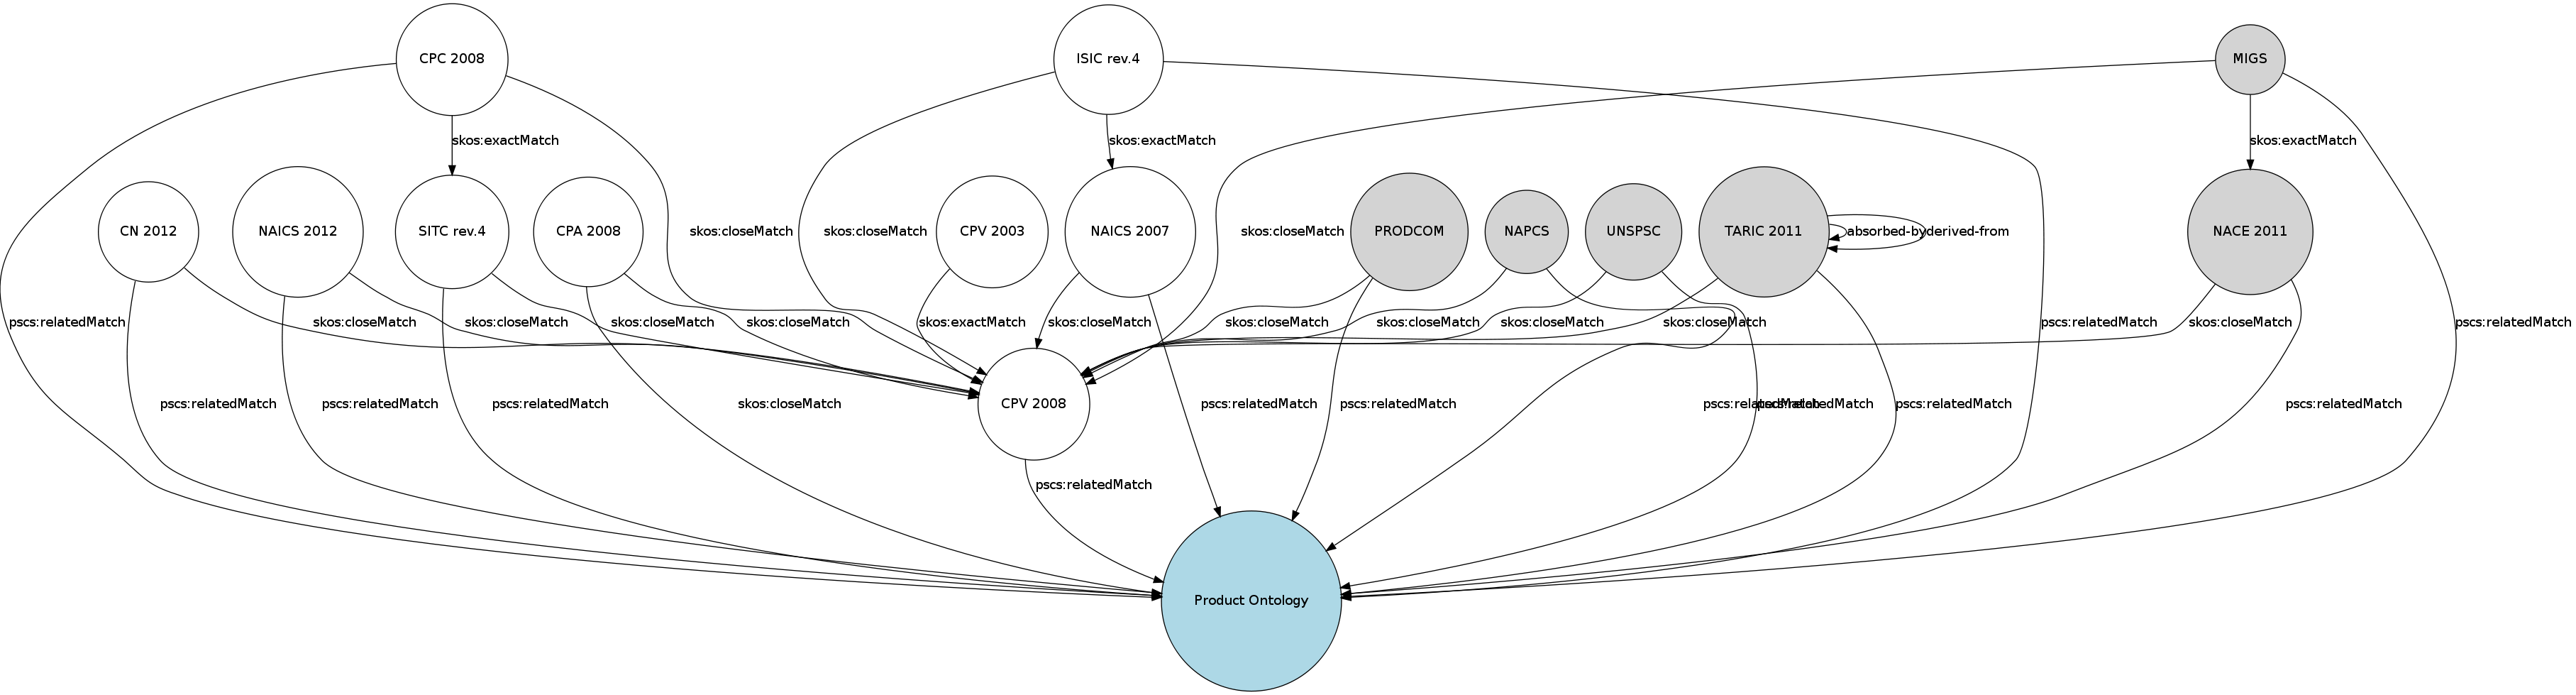
\includegraphics[width=20cm,angle=90]{./images/phd/pscs}
\caption{Enlaces entre las distintas Clasificaciones de Productos.}
\label{fig:linked-pscs}
\end{figure}

\subsubsection{Tarea $t_9$-Transformación de los datos a RDF }
Una vez realizadas las tareas anteriores se está en disposición de realizar la transformación 
de los datos de entrada a \gls{RDF}. En esta tarea el punto clave de decisión reside en seleccionar bien 
una herramienta ya disponible o bien implementar un programa que ejecute las reglas de transformación 
tomando como entrada los datos de las clasificaciones. En el caso objeto de estudio se ha optado 
por un enfoque híbrido realizando la transformación inicial mediante la herramienta Google Refine~\cite{google-refine} y su extensión~\cite{grefine} 
para trabajar con RDF y las posteriores etapas de enriquecimiento a través de una implementación particular que tenga en cuenta 
la casuística específica de las clasificaciones de productos. En cualquier caso, en la ejecución de esta 
tarea se debe asegurar que el \dataset RDF $\mathcal{D}$ generado es válido en cuanto a sintaxis y al modelo definido. Esta tarea 
se ha ejecutado secuencialmente para cada unas de las clasificaciones de productos.
% 
% \begin{figure}[!htb]
% \centering
% 	%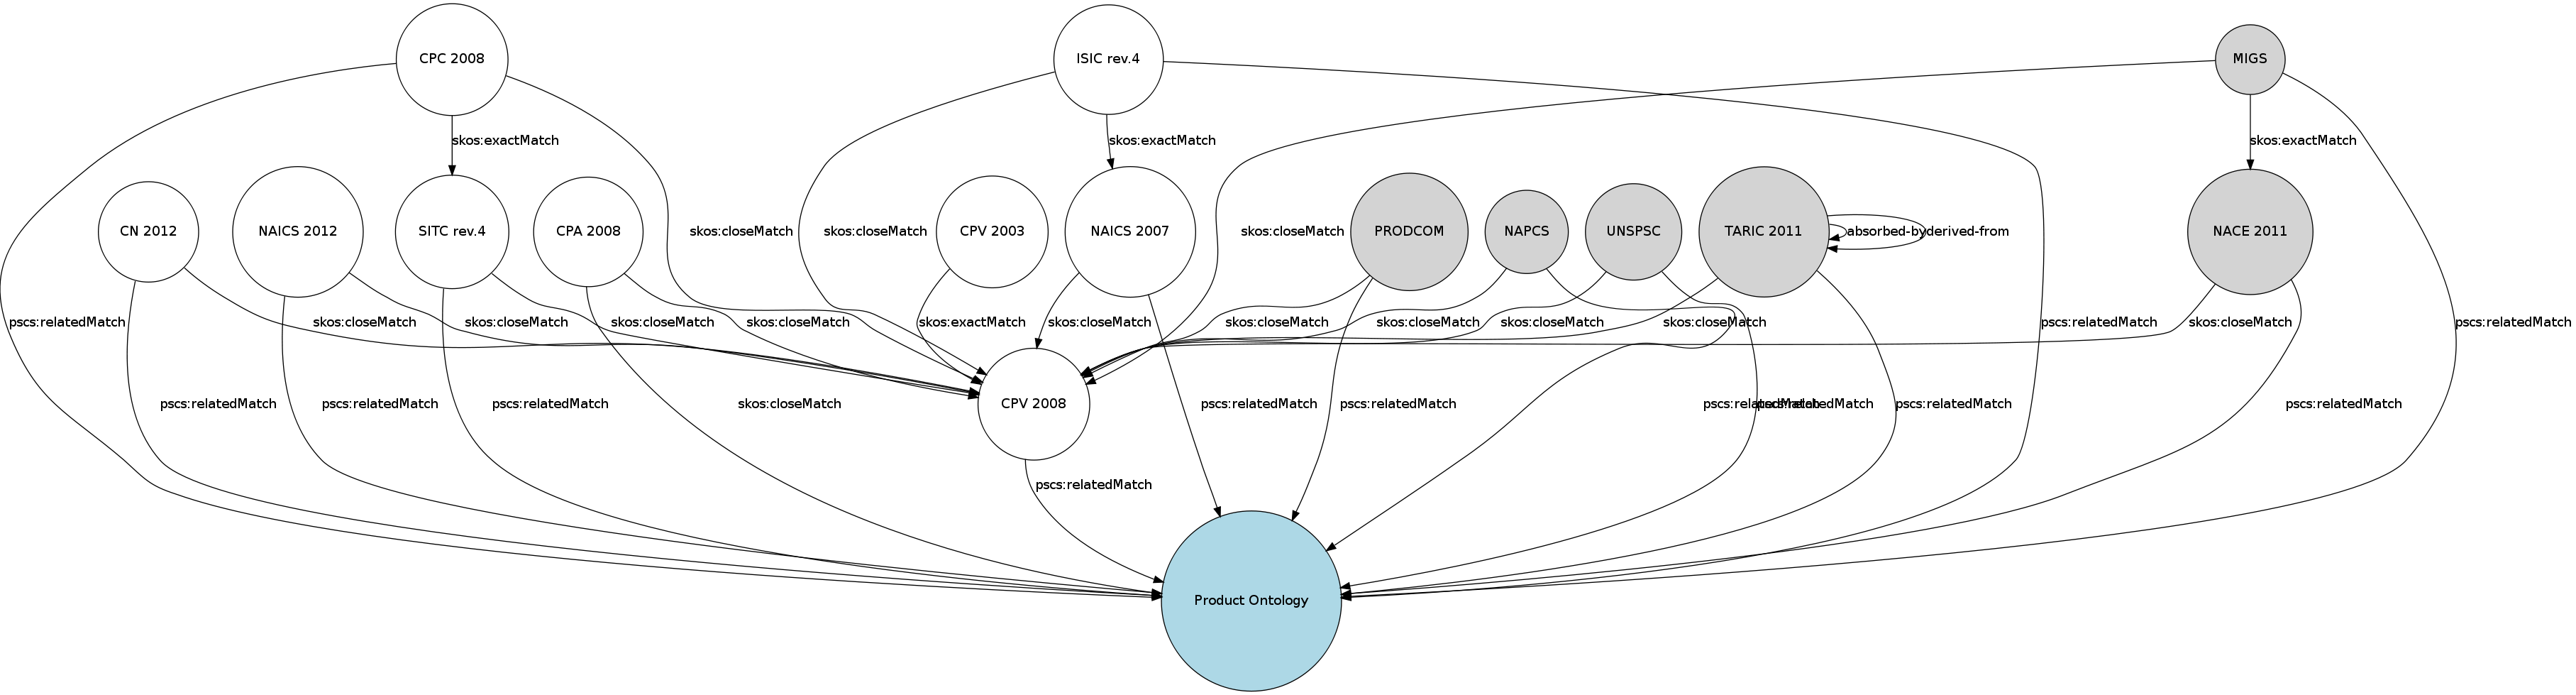
\includegraphics[width=18cm,angle=90]{./images/phd/pscs}
% \caption{Tarea $t_9$-Transformación de los Datos a RDF de las Clasificaciones de Productos.}
% \label{fig:t9-pscs}
% \end{figure}

\subsubsection{Tarea $t_{10}$-Reconciliación de Entidades}
El diseño y ejecución de esta tarea ha sido descrito en la Sección~\ref{t8-pscs} ya que están 
estrechamente ligadas.

\subsubsection{Tarea $t_{16}$-Añadir metainformación a los recursos RDF}\label{t16-pscs}
En el caso de las clasificaciones de productos la metainformación en los recursos se puede 
interpretar en los dos sentidos que se han descrito en la Sección~\ref{t16-metodos}, bien 
en cada uno de los recursos generados o en el \dataset completo. Considerando el carácter 
estático de las clasificaciones de productos en cuanto a su creación, depende de los organismos oficiales que 
se encargan de su mantenimiento, y dado que para los elementos que varían en el tiempo éstos 
generan un \textit{mapeo} directo entre las versiones de los mismos, como en el caso del CPV 2003 y 2008, se considera 
una elección correcta situar la metainformación a nivel de \dataset para cada unas de las PSCs. Para ello y de acuerdo 
a los vocabularios seleccionados se utiliza \textit{\gls{voID}} como especificación para indicar la metainformación 
de un \dataset concreto. El enfoque seguido genera metainformación a nivel del catálogo de las clasificaciones 
de producto, ver Figura~\ref{fig:pscs-ls}, y para cada una de las clasificaciones transformadas, ver Figura~\ref{fig:pscs-ds-cpv-2008} como ejemplo 
de la descripción del \dataset del \gls{CPV} 2008. Es relevante destacar la definición de la licencia de los datos con el objetivo 
de facilitar su posterior reutilización, en este caso se ha optado por una licencia de ``\textit{Open Data}'' basada en las directrices 
fijadas en la guía provista en~\cite{od-license}.

\begin{figure}[!htp]
\begin{lstlisting} 
<http://purl.org/weso/pscs/data/resource/ds?output=ttl>
      rdfs:label "RDF description of Product Scheme Classifications" ;
      foaf:primaryTopic <http://purl.org/weso/pscs/resource/ds> .

<http://purl.org/weso/pscs/resource/ds>
      a    <http://rdfs.org/ns/void#Linkset> ;
      rdfs:label "Product Scheme Classifications"@en ;
      dcterms:author 
            <http://www.di.uniovi.es/~labra/labraFoaf.rdf#me> , 
	    <http://www.josemalvarez.es/foaf.rdf#me> ;
      dcterms:contributor
            <http://purl.org/weso/pscs/resource/10ders> ,
	    <http://rdfohloh.wikier.org/project/moldeas/rdf> ;
      dcterms:description 
            "Some Product Scheme Classifications available in RDF" ;
      dcterms:license
            <http://opendatacommons.org/licenses/by/1.0/> ;
      dcterms:modified
            "2011-11-10"^^<http://www.w3.org/2001/XMLSchema#date> ;
      dcterms:publisher
            <http://www.josemalvarez.es/foaf.rdf#me> ;
       dcterms:title
            "Product Scheme Classifications" ;
      void:target
            <http://purl.org/weso/pscs/cpc/2008/resource/ds> , 
	    <http://purl.org/weso/pscs/naics/2007/resource/ds> , 
	    <http://purl.org/weso/pscs/sitc/v4/resource/ds> , 
	    <http://purl.org/weso/pscs/cpv/2003/resource/ds> , 
	    <http://purl.org/weso/pscs/naics/2012/resource/ds> , 
	    <http://purl.org/weso/pscs/cpv/2008/resource/ds> , 
	    <http://purl.org/weso/pscs/cpa/2008/resource/ds> , 
	    <http://purl.org/weso/pscs/cn/2012/resource/ds> , 
	    <http://purl.org/weso/pscs/isic/v4/resource/ds> ;
      foaf:homepage <http://purl.org/weso> .	
\end{lstlisting}
	\caption{Descripción del \textit{Linkset} de las Clasificaciones Estándar de Productos.}
	\label{fig:pscs-ls}
\end{figure}


\begin{figure}[!htp]
\begin{lstlisting} 
<http://purl.org/weso/pscs/cpv/2008/resource/ds>
      a       void:Dataset , skos:ConceptScheme ;
      rdfs:label "CPV 2008"@en ;
      dcterms:author 
            <http://www.di.uniovi.es/~labra/labraFoaf.rdf#me> , 
	    <http://www.josemalvarez.es/foaf.rdf#me> ;
      dcterms:contributor
            <http://purl.org/weso/pscs/resource/10ders> ,
	    <http://rdfohloh.wikier.org/project/moldeas/rdf> ;
      dcterms:description "Common Procurement Vocabulary" ;
      dcterms:license <http://opendatacommons.org/licenses/by/1.0/> ;
      dcterms:modified "2011-11-10"^^xsd:date ;
      dcterms:publisher <http://www.josemalvarez.es/foaf.rdf#me> ;
      dcterms:source 
	<http://europa.eu/legislation_summaries/internal_market/businesses/public_procurement/l22008_en.htm> ;
      dcterms:title "CPV 2008" ;
      void:dataDump <http://purl.org/weso/pscs/cpv/2008/cpv-2008.ttl> ;
      void:exampleResource
        <http://purl.org/weso/pscs/cpv/2008/resource/18000000> , 
	<http://purl.org/weso/pscs/cpv/2008/resource/45000000> , 
	<http://purl.org/weso/pscs/cpv/2008/resource/33000000> ;
      void:uriRegexPattern
        "http://purl.org/weso/pscs/cpv/2008/resource/.+" ;
      void:vocabulary dc: , skos: , gr: ;
      skos:hasTopConcept 
	<http://purl.org/weso/pscs/cpv/2008/resource/63000000> ,
	<http://purl.org/weso/pscs/cpv/2008/resource/76000000> , 
	<http://purl.org/weso/pscs/cpv/2008/resource/19000000> , 
	<http://purl.org/weso/pscs/cpv/2008/resource/79000000> , 	
	...
	<http://purl.org/weso/pscs/cpv/2008/resource/16000000> ;
      foaf:homepage <http://purl.org/weso> .
\end{lstlisting}
	\caption{Descripción del \dataset CPV 2008.}
	\label{fig:pscs-ds-cpv-2008}
\end{figure}
\clearpage
\subsubsection{Resultado Final y Ejemplos}\label{resultado-pscs}
El resultado final del proceso de producción de \linkeddata, tras el análisis y ejecución 
de las tareas identificadas y del método de producción seleccionado, genera como resultado un catálogo 
de clasificaciones de productos mediante datos enlazados, en los cuales se pueden extraer las siguientes 
estadísticas de producción de datos así como ejemplos de los recursos generados, ver Tabla~\ref{table:pscs-ejemplos}. Por otra parte, 
el aumento de la expresividad en el momento de realizar consultas se puede observar en la Figura~\ref{fig:pscs-sparql-query} en la 
que se expresa la siguiente consulta:

\begin{Frame}
\textit{``Dame 100 productos o servicios relacionados, descripción en inglés, con el término construcción que aparezca en cualquiera de los catálogos disponibles y 
que tengan enlaces con productos o servicios disponibles en la CPV 2008.''}
\end{Frame}


\begin{longtable}[c]{|p{2.5cm}|p{2.5cm}|p{1.8cm}|p{1.8cm}|p{2.5cm}|p{2.5cm}|} 
\hline
  \textbf{Clasificación} & \textbf{Nº de Elementos}  &  \textbf{Ejemplo} &  \textbf{Tripletas} &  \textbf{Enlaces externos} &  \textbf{Enlaces CPV 2008} \\\hline
\endhead
\gls{CPV} 2003 & $8323$  & Figura~\ref{fig:pscs-example-cpv-2003}   & $546135$  & $8322$ & $462$ (del CPV 2008 al 2003)   \\ \hline
CPV 2008 & $10357$ &  Figura~\ref{fig:pscs-example-cpv-2008}   & $803311$  & $10355$ & N/A   \\ \hline
\gls{CN} 2012  & $14552$& Figura~\ref{fig:pscs-example-cn-2012}      & $137484$  & $2590$ & $2390$ \\ \hline
\gls{CPC} 2008 & $4408$&  Figura~\ref{fig:pscs-example-cpc-2008}    & $100819$  & $4408$ & $4375$ y $1503$ (exactos)  \\ \hline
\gls{CPA} 2008 & $5429$&  Figura~\ref{fig:pscs-example-cpa-2008}    & $92749$   & $5429$ & $5399$  \\ \hline
\gls{ISIC} v4  & $766$& Figura~\ref{fig:pscs-example-isic-rev4}    & $18986$   & $766$ & $765$  \\ \hline
\gls{NAICS} 2007 & $2328$& Figura~\ref{fig:pscs-example-naics-2007} & $36292$   & $2328$ & $2300$  \\ \hline
NAICS 2012 & $2212$& Figura~\ref{fig:pscs-example-naics-2012} & $35390$   & $2212$ & $2186$  \\ \hline
\gls{SITC} v4 & $4017$&  Figura~\ref{fig:pscs-example-sitc-v4}      & $70887$   & $3941$ & $3811$  \\ \hline
\multicolumn{6}{|c|}{\textbf{Catálogo de Clasificaciones Estándar de Productos} (total)} \\ \hline
PSCs & $52392$ &  N/A & $1842053$ & $40351$ & $23191$  \\ \hline
\hline
\caption{Estadísticas y Ejemplos del Catálogo de Clasificaciones Estándar de Productos seleccionadas.}\label{table:pscs-ejemplos}\\    
\end{longtable}

\begin{figure}[!htp]
\begin{lstlisting} 
SELECT DISTINCT * WHERE{
  ?product pscs:relatedMatch <http://www.productontology.org/id/construction> .
  ?product skos:closeMatch ?cpv.
  ?product skos:prefLabel ?productLabel.
  ?cpv skos:prefLabel ?cpvLabel.
  ?product skos:inScheme ?scheme.
  FILTER (?scheme != <http://purl.org/weso/pscs/cpv/2008/resource/ds>).
  FILTER (lang(?cpvLabel)="en")
} LIMIT 100
\end{lstlisting}
	\caption{Ejemplo de consulta en SPARQL sobre el Catálogo de Clasificaciones de Productos.}
	\label{fig:pscs-sparql-query}
\end{figure}

\begin{figure}[!htp]
\lstinputlisting{examples/e-proc/cpv-2003.ttl}
	\caption{Ejemplo final de un Recurso del CPV 2003.}
	\label{fig:pscs-example-cpv-2003}
\end{figure}

\begin{figure}[!htp]
	\lstinputlisting{examples/e-proc/cpv-2008.ttl}
	\caption{Ejemplo final de un Recurso del CPV 2008.}
	\label{fig:pscs-example-cpv-2008}
\end{figure}

\begin{figure}[!htp]
\lstinputlisting{examples/e-proc/cn-2012.ttl}
	\caption{Ejemplo final de un Recurso de CN 2012.}
	\label{fig:pscs-example-cn-2012}
\end{figure}

\begin{figure}[!htp]
\lstinputlisting{examples/e-proc/cpc-2008.ttl}
	\caption{Ejemplo final de un Recurso de CPC 2008.}
	\label{fig:pscs-example-cpc-2008}
\end{figure}


\begin{figure}[!htp]
\lstinputlisting{examples/e-proc/cpa-2008.ttl}
	\caption{Ejemplo final de un Recurso de CPA 2008.}
	\label{fig:pscs-example-cpa-2008}
\end{figure}


\begin{figure}[!htp]
\lstinputlisting{examples/e-proc/isic-v4.ttl}
	\caption{Ejemplo final de un Recurso de ISIC rev4.}
	\label{fig:pscs-example-isic-rev4}
\end{figure}


\begin{figure}[!htp]
\lstinputlisting{examples/e-proc/naics-2007.ttl}
	\caption{Ejemplo final de un Recurso de NAICS 2007.}
	\label{fig:pscs-example-naics-2007}
\end{figure}


\begin{figure}[!htp]
\lstinputlisting{examples/e-proc/naics-2012.ttl}
	\caption{Ejemplo final de un Recurso de NAICS 2012.}
	\label{fig:pscs-example-naics-2012}
\end{figure}


\begin{figure}[!htp]
\lstinputlisting{examples/e-proc/sitc-v4.ttl}
	\caption{Ejemplo final de un Recurso de SITC v4.}
	\label{fig:pscs-example-sitc-v4}
\end{figure}


\clearpage
\subsubsection{Método de Producción de \linkeddata de Clasificaciones Estándar de Productos}
De acuerdo al análisis y diseño de datos enlazados realizado para las clasificaciones de productos 
a lo largo de las anteriores anteriores y la tabla de decisión~\ref{tabla:produccion}, el método semántico seleccionado 
para realizar la producción de datos enlazados es el $SPM_1$-``Transformación de datos a RDF'', ver Sección~\ref{spm-1}, en el 
se transforman un conjunto de datos de entrada $\mathcal{G}$ a un \dataset \gls{RDF} $\mathcal{D}$. Según la definición de método 
semántico de producción, realizada en la Sección~\ref{method-prod-def}, y el estudio de las clasificaciones de productos se pueden 
establecer los siguientes conjuntos:
\begin{itemize}
 \item $\mathcal{G}$ es el \dataset de entrada, conjunto de tuplas, conteniendo los datos de cada una de las clasificaciones de productos.
 \item $\mathcal{M}$ es el conjunto de \textit{mapeos}, ver Tabla~\ref{table:pscs-mappings}, extraídos según el análisis y diseño realizado en las secciones anteriores. Estos 
\textit{mapeos} son directamente expresables en la herramienta de transformación y toman como parámetros el valor de una de las tuplas de entrada (posición $X$) y la propiedad a generar.
 \item \textit{Dataset} RDF $\mathcal{D}$ es el \dataset resultado, siguiendo el análisis y diseño realizado en las secciones anteriores y tras la ejecución 
de la tarea propia de transformación de datos.
\end{itemize}

\begin{longtable}[c]{|p{2cm}|p{8cm}|p{4cm}|} 
\hline
  \textbf{$\mathcal{M}$} &  \textbf{Propiedad} & \textbf{Valor} \\\hline
\endhead
 $m_1$ & \texttt{rdf:type} & \gls{URI} \\ \hline
 $m_2$ & \texttt{skos:inScheme} & URI  \\ \hline
 $m_3$ & \texttt{dc:identifier} & \texttt{xsd:string} \\ \hline
 $m_4$ & \texttt{dc:subject} & \texttt{xsd:string} \\ \hline
 $m_5$ & \texttt{pscs:relatedMatch} & URI  \\ \hline
 $m_6$ & \texttt{skos:exactMatch } & URI \\ \hline
 $m_7$ & \texttt{skos:closeMatch } & URI  \\ \hline
 $m_8$ & \texttt{pscs:level} & \texttt{xds:int} \\ \hline  
 $m_9$ & \texttt{skos:broaderTransitive} & URI \\ \hline
 $m_{10}$ & \texttt{skos:prefLabel}, \texttt{rdfs:label}, \texttt{gr:description}  & \texttt{xsd:string@lang} \\ \hline   
\hline
\caption{Conjunto de \textit{mapeos} $\mathcal{M}$ para las Clasificaciones Estándar de Productos.}\label{table:pscs-mappings}\\    
\end{longtable}

\subsection{Proceso de Publicación de \linkeddata de Clasificaciones\\ Estándar de Productos}\label{sect:proceso-publicacion-ld}
Considerando que la estrategia definida para todos los \datasets implicados en el proceso de contratación pública 
electrónica es común, el proceso de publicación es homogéneo siguiendo la estructura definida 
en la Sección~\ref{sect:proceso-publicacion-ld}.

\newpage

\subsubsection{Tarea $t_{14}$-Infraestructura para \linkeddata}
Nuevamente, la estrategia definida para todos los \datasets implicados en el proceso de contratación pública 
electrónica es común, por ello la infraestructura utilizada es la misma que la definida 
en la Sección~\ref{infraestructura-comun}.

\subsubsection{Tarea $t_{15}$-Acceso y formato en datos RDF}
De la misma forma que en el apartado anterior, el acceso y formato de datos RDF para los datos contenidos y relativos 
a las organizaciones siguen el esquema proporcionado en la Sección~\ref{t15-comun}.

\subsection{Proceso de Consumo de Clasificaciones Estándar\\ de Productos}
El proceso de consumo de datos enlazados, según la definición realizada en la Sección~\ref{sect:proceso-consumo}, consiste en 
la reutilización de los datos enlazados para ser aplicados en la construcción de una nueva aplicación o servicio de valor 
añadido. En general, la reutilización más sencilla consiste en la representación gráfica de los recursos o la simple 
consulta con selección de formato de datos de acuerdo a las características de publicación utilizadas. En el caso 
que nos ocupa y teniendo en cuenta el objetivo de realización de un prototipo experimental de extracción de anuncios 
de licitación como demostrador del consumo de datos enlazados, se ha escogido el método semántico de consumo $SCM_2$-``\textit{Mapeo} a Lenguaje de Programación'', 
cuya descripción está disponible en la Sección~\ref{scm2-consumo}, orientado a obtener una representación de los recursos RDF en un 
lenguaje de programación (en este caso Java) como objetos de negocio. De acuerdo a este objetivo y la definición del propio método 
es necesario definir:
\begin{itemize}
 \item El \dataset RDF $\mathcal{D}_{pub}$, es el conjunto de datos disponible tras aplicar el método de publicación.
 \item El conjunto $\mathcal{M}^1$, ver Tabla~\ref{table:pscs-consumo}, indica como transformar el \dataset anterior a la representación objetivo, objetos del lenguaje Java.
\end{itemize}

De esta manera, se obtiene una serie de objetos, $\mathcal{D}_{consum}$, con la información y datos necesarios, no se transforman necesariamente todos los datos disponibles en los recursos pertenecientes 
a  $\mathcal{D}_{pub}$, para ser reutilizados como objetos de negocio en un lenguaje de programación. Es conveniente señalar que el acceso a los datos se realiza a través 
de la consulta al \textit{endpoint} de \gls{SPARQL} ejecutando consultas \textit{SELECT} y \textit{DESCRIBE}.

\begin{longtable}[c]{|p{2cm}|p{6cm}|p{6cm}|} 
\hline
  \textbf{$\mathcal{M}^1$} &  \textbf{Propiedad} & \textbf{Tipo en Java} \\\hline
\endhead
 $m^1_1$ & URI recurso     		& \texttt{java.lang.String} \\ \hline
 $m^1_2$ & \texttt{rdf:type}      	& \texttt{org.weso.moldeas.to.PSCTO} \\ \hline
 $m^1_3$ & \texttt{skos:inScheme} 	& \texttt{java.lang.String}  \\ \hline
 $m^1_4$ & \texttt{dc:identifier} 	& \texttt{java.lang.String} \\ \hline
 $m^1_5$ & \texttt{dc:subject}    	& \texttt{java.lang.String} \\ \hline
 $m^1_6$ & \texttt{pscs:relatedMatch} 	& \texttt{java.util.List<PSCTO> } \\ \hline
 $m^1_7$ & \texttt{skos:exactMatch } 	& \texttt{java.util.List<PSCTO> }\\ \hline
 $m^1_8$ & \texttt{skos:closeMatch } 	& \texttt{java.util.List<PSCTO>}  \\ \hline
 $m^1_9$ & \texttt{pscs:level} 	& int \\ \hline  
 $m^1_{10}$ & \texttt{skos:broaderTransitive} & java.util.List<PSCTO>  \\ \hline
 $m^1_{11}$ & \texttt{skos:prefLabel}, \texttt{rdfs:label}, \texttt{gr:description}  & Map<String,String> (lang, value) para cada propiedad \\ \hline   

\hline
\caption{Conjunto de \textit{mapeos} $\mathcal{M}^1$ de consumo para las Clasificaciones Estándar de Productos.}\label{table:pscs-consumo}\\    
\end{longtable}

\subsection{Proceso de Validación de Clasificaciones Estándar de Productos}
La validación como proceso transversal en cualquier etapa dentro del ciclo de vida de datos 
enlazados debe realizarse con el objetivo de asegurar la calidad de los datos. De acuerdo a la 
definición realizada en la Sección~\ref{sect:validation}, este proceso consiste en la comprobación 
de que los recursos de un \dataset RDF cumplen ciertas características. 

La realización de esta validación puede ser realizada manual o automáticamente en función del caso concreto, por ejemplo para la característica 
de negociación de contenido o para la inclusión en la nube de datos enlazados se dispone de herramientas adecuadas, pero 
en cambio para comprobaciones relativas a los dominios y rangos de las propiedades, etc., no existe una 
herramienta completa. Por todo ello, se ha seguido un enfoque híbrido basado en la utilización de herramientas 
y validación manual. La descripción completa de la validación de acuerdo a todas las características 
se reseña en las Tablas de Validación disponibles en el Apéndice~\ref{tablas-validacion-apen}.

\subsubsection{Tarea $t_{12}$-Validación de Recursos RDF}
Siguiendo con la definición realizada de esta tarea en la Sección~\ref{lod-t12}, se puede asegurar que la transformación 
realizada de los catálogos de clasificaciones de productos a la iniciativa \linkeddata cumple estrictamente los 
siguientes puntos:

\begin{itemize}
 \item Los datos \gls{RDF} son correctos ya que se han utilizado herramientas y \gls{API}s (Google \gls{Refine} y Jena) que aseguran 
la generación correcta de RDF.
 \item El dominio y rango en las propiedades es correcta, ya que se realiza la validación contra el modelo definido.
 \item Se ha establecido metainformación sobre la procedencia a nivel de \dataset.
 \item Todos los recursos transformados siguen la plantilla objetivo RDF.
\end{itemize}

\subsection{Proceso de Realimentación de Clasificaciones\\ Estándar de Productos}
Este proceso según la definición realizada en la Sección~\ref{proceso-realimentacion}, busca la mejora 
y perfeccionamiento de los datos promocionados a \gls{RDF}. Esta situación emerge en el momento en el cual 
los datos comienzan a ser reutilizados, tanto por aplicaciones o servicios como por individuos. En el caso 
particular del catálogo de las clasificaciones de productos y debido a su reutilización por la 
\textit{Charles University} de la República Checa se han detectado errores que han sido 
corregidos, se trata de casos específicos no detectados por el proceso de validación, debido al procesamiento masivo de datos. 
En este sentido el proceso de realimentación se basa en un enfoque en el cual \textit{Usuarios y Aplicaciones} realizan 
el descubrimiento de datos no correctos y cuyo cambio se centra en una \textit{Actualización Ocasional}. Aunque 
este enfoque es completamente válido, es conveniente señalar que este proceso todavía no se ha definido de forma 
completa dentro de la iniciativa de \linkeddata por lo que su ejecución automática constituye un objetivo 
a medio plazo en el que terceros puedan mejorar los datos previa validación del \textit{Propietario de datos}.
\section{Organizaciones}\label{sect:rdf-orgs}
La información de las organizaciones se considera un punto clave para la realización 
de muchos servicios de valor añadido tanto para la Administración Pública como 
para otras entidades. El conocimiento del estado financiero de una entidad, la actividad que ha desarrollado a 
través de proyectos, los productos y servicios ofertados, el listado de clientes y socios, etc., se considera una 
información de alto interés para la monitorización y la selección de posibles entidades 
para el establecimiento de relaciones de negocios. Desde el punto de vista interno de la propia organización, su estructura y 
personas implicadas en el desarrollo de la actividad de negocio así como la explotación del conocimiento organizacional 
son factores clave que determinan el camino a seguir por una entidad y su valor como tal. Como se ha señalado 
en la Sección~\ref{sect:orgs}, existen varios enfoques para la representación de la información de las organizaciones, 
en el caso objeto de estudio de este documento se centrará principalmente en los siguientes puntos: 1) información 
de contacto de la organización respecto a su localización y 2) persona de referencia para el establecimiento de 
relaciones. Este planteamiento es válido tanto para la representación de la información de los organismos que, cuentan con capacidad 
para la realización de contratos públicos, como para aquellos que deseen concursar a través de ofertas y cuya información 
debe perdurar a lo largo del tiempo hasta el fin del contrato. De acuerdo a la información disponible en las distintas 
fuentes de información de los anuncios de licitación las organizaciones o entidades modeladas cumplirán, al menos, con estos 
dos puntos clave que suponen un gran avance respecto a la información actual.

\subsection{Proceso de Producción de \linkeddata de Organizaciones}
Al igual que en el caso de las clasificaciones de productos y según la definición realizada 
de este proceso en la Sección~\ref{sect:produccion}, este proceso implica todas las tareas 
que se han de realizar para la transformación de un \dataset de entrada $\mathcal{G}$, mediante 
unas reglas de \textit{mapeo} $\mathcal{M}$, con el objetivo de conseguir un \dataset \gls{RDF} $\mathcal{D}$, de esta forma 
se define el método semántico de producción. 

\subsubsection{Tarea $t_1$-Análisis del \dataset a transformar}\label{t1-orgs}
Las organizaciones, tanto órganos contrantes como ofertantes, durante el proceso administrativo de 
contratación pública generan información y datos abarcando un amplio espectro, sin embargo para los fines 
de apertura y enlazado de datos mediante un modelo formal se considera 
suficiente la representación de la información de contacto de una entidad, 
incluyendo tanto a la persona física o jurídica de la misma con especial atención a su localización. La realidad 
es que la obtención de la información y datos pormenorizados de una organización se haya disponible públicamente, 
pero a través de fuentes información de difícil consulta que carecen de relevancia crítica para el estudio realizado en este trabajo, 
por ello se ha decidido realizar un primer acercamiento a la información empresarial focalizando el esfuerzo en la selección 
de un modelo formal que suministre el marco de trabajo adecuado para la representación de información 
de las organizaciones de una forma sencilla y operativa en el ámbito de la contratación pública 
electrónica. En este sentido, emergen tres entidades: organizaciones, personas y países, en las que 
hay que representar distintos datos, principalmente en las dos primeras información relativa a los datos de contacto y en la última 
la geolocalización. Una organización puede tener diferentes identificadores, asumiendo que cada uno de sus departamentos o 
subdivisiones y también las personas varían de acuerdo a la unidad mínima de organización seleccionada 
y en consecuencia su localización. La invariante que se produce reside en que para un proceso de contratación pública, la tupla 
una organización (entidad, departamento, división, etc.), una persona de contacto, un país y un propósito determinado es única.

En este sentido, surge la necesidad de especificar las organizaciones, personas, direcciones y países en un modelo formal. Para 
la utilización de un modelo formal, extensible que suministre el soporte necesario para el almacenamiento de la información y datos de las entidades con carácter 
multiling\"{u}e, se ha seleccionado la ontología ``\textit{Organizations}'' realizada por \textit{Dave Reynolds} (Epimorphics Ltd) ya que conjuga 
los esfuerzos de anteriores propuestas facilitando la representación de cualquier tipo de entidad desde un punto de vista 
estructural, información de contacto, actividad desarrollada, etc., convirtiéndose de esta manera en el marco de trabajo 
apropiado para el tratamiento de la información de licitantes y licitadores. La información sobre las personas se representa con la ontología 
FOAF, mientras que finalmente los países y su información, además de utilizar el \dataset de NUTS (regiones de Europa), reutilizan 
las definiciones realizadas en la DBPedia. 

La información que se tomará como paradigmática para este enfoque surge de las hojas de cálculo disponibles en el servidor 
\gls{FTP} de \gls{TED} en la Unión Europea, que consta de los siguientes campos: \textit{organisation official name, postal address (street), town, 
postalcode, countrycode, contact: attention, tel, fax, email, url, postal-code for the country (1 to 3 characters), contact point(s): telephone number, 
fax number, e-mail address, \gls{URL}}, un ejemplo completo se ha señalado en la Figura~\ref{fig:orgs-example-ted} extraído 
de la documentación oficial de TED. No obstante y de acuerdo a la ejecución del proyecto ``10ders Information Services'' se ha seleccionado 
el \dataset provisto por la empresa Gateway S.C.S., reseñado en la Figura~\ref{fig:orgs-example}, y consistente en $50,000$ entidades. La actualización 
de este \dataset es incremental a lo largo del tiempo y crece generando una gran masa de información de datos, con el objetivo de realizar la prueba 
de concepto de representación de la información empresarial, se ha decidido acotar a las necesidades del proyecto.

\begin{figure}[!htp]
\begin{lstlisting} 
<addr>
  <organisation>Westminster City Council</organisation>
  <address>City Hall, 64 Victoria Street</address>
  <contact>Westminster Accord</contact>
  <attention>Linda Pinder</attention>
  <countrycode>UK</countrycode>
  <town>London</town>
  <postalcode>SW1E 6QP</postalcode>
  <tel>020 7641 3173</tel>
  <email><txemail>lpinder@westminster.gov.uk</txemail></email>.
  <fax>020 7641 3017</fax>
</addr>
\end{lstlisting}
	\caption{Ejemplo de datos sobre una Organización en TED.}
	\label{fig:orgs-example-ted}
\end{figure}


\begin{figure}[!htp]
\begin{lstlisting} 
ID contrato, ISO code, campos internos de la BBDD, tipo de entidad, nombre entidad en cada idioma, dir. postal, campos de la dir. postal
...
000170-2011,da,false,7,5,1,ContractingAuthority,Europa-Parlamentet,,,"plateau de Kirchberg, 2929, Luxembourg",plateau de Kirchberg,2929,Luxembourg,,"",,,
000170-2011,lv,false,7,5,1,ContractingAuthority,Eiropas Parlaments,,,"plateau de Kirchberg, 2929, Luksemburga",plateau de Kirchberg,2929,Luksemburga,,"",,,
000170-2011,nl,false,7,5,1,ContractingAuthority,Europees Parlement,,,"plateau de Kirchberg, 2929, Luxemburg",plateau de Kirchberg,2929,Luxemburg,,"",,,
000170-2011,pl,false,7,5,1,ContractingAuthority,Parlament Europejski,,,"plateau de Kirchberg, 2929, Luksemburg",plateau de Kirchberg,2929,Luksemburg,,"",,,
000170-2011,pt,false,7,5,1,ContractingAuthority,Parlamento Europeu,,,"plateau de Kirchberg, 2929, Luxemburgo",plateau de Kirchberg,2929,Luxemburgo,,"",,,
000170-2011,es,false,7,5,1,ContractingAuthority,Parlamento Europeo,,,"plateau de Kirchberg, 2929, Luxemburgo",plateau de Kirchberg,2929,Luxemburgo,,"",,,
...
\end{lstlisting}
	\caption{Ejemplo de datos sobre Organizaciones.}
	\label{fig:orgs-example}
\end{figure}


\subsubsection{Tarea $t_2$-Limpieza de datos}
La oportunidad de reutilizar la información y datos suministrados por una empresa experta en el dominio de la 
contratación pública y con la capacidad para filtrar aquella información y datos relevantes resulta de gran 
valor para la ejecución de la transformación de estos datos. Es por ello que partiendo de este \dataset 
original, esta tarea ya ha sido realizada y los datos a transformar se encuentran en condiciones óptimas 
de calidad, tanto en contenido como en formato (\gls{CSV}).

\subsubsection{Tarea $t_3$-Selección de Vocabularios}
Los vocabularios seleccionados para modelar la información de las organizaciones teniendo en cuenta el análisis 
realizado en la tarea $t_1$ y la metodología seguida en los anteriores apartados se presentan en la Tabla~\ref{table:orgs-select-vocabs}. 
En general, se trata de vocabularios que atienden a los siguientes criterios:

\begin{enumerate}
 \item Formalización de una estructura taxonómica, como RDFS, \gls{SKOS} u \gls{OWL}.
 \item Realización de \textit{mapeos} entre conceptos, como SKOS y OWL.
 \item Representación de tipos de datos, como \gls{XML Schema}.
 \item Gestión de información multiling\"{u}e, como SKOS-XL y RDFS.
 \item Representación de información de negocio (entidades y personas), como ``\textit{Organizations Ontology}'', ``\gls{FOAF}'' y ``\textit{DBPedia Ontology}''.
 \item Adición de metadatos y provenance, como \textit{Dublin Core Terms}, \gls{voID} y \textit{Provenance Ontology}.
 \item Representación de información de contacto como vCard en RDF.
\end{enumerate}


\begin{longtable}[c]{|l|p{4cm}|p{4cm}|p{4cm}|} 
\hline
\textbf{Prefijo} &  \textbf{Vocabulario} &  \textbf{Fuente} & \textbf{Uso} \\\hline
\endhead
 dbpedia & \url{http://dbpedia.org/ontology/}&  Comunidad \linkeddata. & Reutilización de definiciones. \\ \hline 
 dc & \url{http://purl.org/dc/elements/1.1/}&  \textit{Dublin Core Metadata Initiative} & Creación de metadatos para los documentos. \\ \hline  
 dct & \url{http://dublincore.org/documents/dcmi-terms/}&  $\equiv$ & $\equiv$ \\ \hline  
 foaf & \url{http://xmlns.com/foaf/0.1/} &Comunidad de Web Semántica.& Especificación de relaciones entre personas. \\ \hline 
 geo & \url{http://www.w3.org/2003/01/geo/wgs84_pos#} & W3C & Reutilización de elementos geográficos.\\\hline 
 lgd & \url{http://linkedgeodata.org/ontology/} & \textit{Linked Geodata Initiative} & $\equiv$\\\hline 
 org  & \url{http://www.w3.org/ns/org#} & W3C y Epimorphics Ltd. & Descripción de organizaciones. \\ \hline
 owl  & \url{http://www.w3.org/2002/07/owl#} & W3C & Realización de definiciones en el dominio. \\\hline
 prov  & \url{http://purl.org/twc/ontology/w3c/prov#} & W3C & Especificación de metadatos de procedencia. \\\hline 
 nuts  & \url{http://nuts.psi.enakting.org/def/} & Universidad de Southampton & Especificación de las regiones europeas. \\\hline
 skos & \url{http://www.w3.org/2004/02/skos/core#} & W3C & Especificación de taxonomías. \\ \hline
 skosxl & \url{http://www.w3.org/2008/05/skos-xl#>} & W3C & Representación de información ling\"uística. \\ \hline
 rdf & \url{http://www.w3.org/1999/02/22-rdf-syntax-ns#} & W3C & Descripción de recursos. \\ \hline
 rdfs & \url{http://www.w3.org/2000/01/rdf-schema#} & W3C & Descripción de recursos con relaciones lógicas. \\ \hline 
 vcard & \url{http://www.w3.org/2006/vcard/ns#} & W3C & Representación de información de contacto. \\\hline
 void & \url{http://rdfs.org/ns/void#} & Deri y W3C & Descripción de metadatos de un \dataset. \\\hline
 xml & \url{http://www.w3.org/XML/1998/namespace} & W3C & Reutilización de definiciones. \\\hline
 xsd & \url{http://www.w3.org/2001/XMLSchema#} & W3C & Especificación de tipos de datos. \\\hline
\hline
\caption{Selección de Vocabularios para las Organizaciones.}\label{table:orgs-select-vocabs}\\    
\end{longtable}

\subsubsection{Tarea $t_4$-Selección de otros \datasets RDF}
En este caso los \datasets a reutilizar se centran en la información sobre personas y organizaciones, otorgando 
igualmente valor a la información sobre países, específicamente a las regiones europeas. Los conjuntos de datos 
seleccionados se señalan en la Tabla~\ref{table:orgs-select-datasets}.

\begin{longtable}[c]{|l|p{4cm}|p{4cm}|p{4cm}|} 
\hline
  \textbf{Prefijo} &  \textbf{\textit{Dataset}} &  \textbf{Fuente} & \textbf{Uso} \\\hline
\endhead
dbpedia-res & \url{http://dbpedia.org/}&  Comunidad \linkeddata. & Reutilización de datos provenientes de la DBPedia. \\ \hline 
nuts & \url{http://nuts.psi.enakting.org/} & University of Southampton & Especificación de las regiones europeas.\\\hline 
\hline
\caption{Selección de otros \datasets para las Organizaciones.}\label{table:orgs-select-datasets}\\    
\end{longtable}


\subsubsection{Tarea $t_5$-Modelado de datos en RDF}
El resultado de esta tarea debe ser una ontología de dominio $\mathcal{O}$ que modele los recursos, organizaciones, personas y países, pertenecientes a un 
\dataset \gls{RDF} $\mathcal{D}$. Inicialmente, se debe proveer la especificación del modelo 
formal u ontología $\mathcal{O}$ de acuerdo al análisis realizado en la tarea $t_1$, dando soporte a la descripción de los datos de los recursos RDF:

\begin{itemize}
 \item $\mathcal{C} = \{$\textit{Organization, Country, Person,\ldots, Site}$\}$
 \item $\mathcal{R} = \{$\textit{rdf:type, dc:identifier, org:purpose, org:classification,\ldots, org:memberOf, rdfs:label}$\}$
 \item $\mathcal{I} = \{ r_{org}, r_{country} \}$
 \item $\mathcal{A} = \{\star\}$, son los axiomas propios de la ontología de organizaciones y los vocabularios FOAF y vCard.
\end{itemize}
 
Como segundo paso se diseñan las propiedades que deben tener los recursos, teniendo en cuenta su ulterior aplicación ver Tabla~\ref{table:orgs-rdf-model}, 
pertenecientes a ese \dataset (organizaciones, personas y países).

\begin{longtable}[c]{|p{4cm}|p{5.5cm}|p{5cm}|} 
\hline
  \textbf{Propiedad} &  \textbf{Descripción} & \textbf{Ejemplo} \\\hline
\endhead
  \texttt{rdf:type} & Especificación del tipo de un recurso & \texttt{org:FormalOrganization}  \\ \hline
  \texttt{rdfs:label} & Etiqueta para el recurso organización, persona o país &   \texttt{rdfs:label} "Dutch Company Inc."@en  \\ \hline  
  \texttt{org:purpose} & Perfil de características de una organización &   N/A\\ \hline
  \texttt{org:classification} & Tipo de organización de acuerdo a una taxonomía en \gls{SKOS} &  \texttt{org:classification} <SME> \\ \hline
  \texttt{org:hasSite} & Localización física de una organización  &  \texttt{org:hasSite} \url{<http://purl.org/weso/eprocurement/organization/resource/{id}/site>} \\ \hline
  \texttt{org:siteAddress} & Recurso \texttt{vcard} que especifica los datos de una localización física de una organización o persona & \texttt{org:siteAddress} \url{<http://purl.org/weso/eprocurement/organization/resource/{id}/vcard>}   \\ \hline
  \texttt{org:memberOf} & Pertenencia de un ``agente'', en este caso personas a una organización &   \\ \hline
  \texttt{org:basedAt} &  Localización física de una persona  &  \texttt{org:basedAt} \url{<http://purl.org/weso/eprocurement/organization/resource/{id}/vcard>} \\ \hline
  \texttt{ref-country} & Enlace a un país & \texttt{ref-country} \url{<http://purl.org/weso/eprocurement/country/resource/ES>}  \\ \hline 
  \texttt{ref-dbpedia} & Enlace al recurso de un país en la DBPedia &  \texttt{ref-dbpedia} \url{<http://dbpedia.org/resource/ISO_3166-1:ES>} \\ \hline
  \texttt{located-in} & Enlace al recurso de una región en NUTS & \texttt{located-in} \url{<http://nuts.psi.enakting.org/id/ES>}  \\ \hline  
  \texttt{short-label} & Código \gls{ISO} 3166 de un país &  \texttt{short-label} ``ES'' \\ \hline
  \texttt{geo:lat} & Latitud de un recurso & \texttt{geo:lat} ``40.46366700000001''  \\ \hline
  \texttt{geo:long} & Longitud de un recurso &  \texttt{geo:long} ``-3.74922''  \\ \hline
  \texttt{vcard:*} & Establecimiento de la información de contacto para un recurso organización o persona &  N/A \\ \hline
\hline
\caption{Diseño de propiedades para los elementos de las Organizaciones.}\label{table:orgs-rdf-model}\\    
\end{longtable}

Una vez especificado el conjunto de propiedades de cada recurso es necesario definir el conjunto 
de grafos en los cuales se encuadrarán los recursos, es decir, el \dataset \gls{RDF} $\mathcal{D}$. Para ello, 
en la Tabla~\ref{table:orgs-dataset} se indican las tuplas $(\mathcal{G}_k, I_k)$ correspondientes a cada uno 
de los grafos $\mathcal{G}_k$ identificados a través de la \gls{URI} $I_k$ realizando especial énfasis en la separación 
entre los recursos con datos en sí mismos, de las definiciones de aquellos. Hay que destacar que los recursos 
de la información asociada a personas no tienen entidad por sí mismos sino que se relacionan con una organización, es decir, 
no existen personas no relacionadas con organizaciones.

\begin{longtable}[c]{|p{3cm}|p{9cm}|} 
\hline
  \textbf{$\mathcal{G}_k$} &  \textbf{$I_k$}  \\\hline
\endhead
 \textbf{$\mathcal{G}$}     & \url{http://purl.org/weso/eprocurement/} \\ \hline
 \textbf{$\mathcal{G}_{1}$} & \url{http://purl.org/weso/eprocurement/organization} \\ \hline
 \textbf{$\mathcal{G}_{2}$} & \url{http://purl.org/weso/eprocurement/organization/person/} \\ \hline
 \textbf{$\mathcal{G}_{3}$} & \url{http://purl.org/weso/eprocurement/country} \\ \hline
 \textbf{$\mathcal{G}_{4}$} & \url{http://purl.org/weso/eprocurement/organization/ontology} \\ \hline
 \textbf{$\mathcal{G}_{5}$} & \url{http://purl.org/weso/eprocurement/country/ontology} \\ \hline 
\hline
\caption{\textit{Dataset} RDF $\mathcal{D}$ para Organizaciones.}\label{table:orgs-dataset}\\    
\end{longtable}


\subsubsection{Tarea $t_6$-Diseño de un Esquema de URIs}
Esta tarea tiene como objetivo establecer la forma y estructura de las \gls{URI}s tanto para las definiciones 
realizadas en la ontología $\mathcal{O}$ como para todos los recursos presentes en el \dataset RDF $\mathcal{D}$ que 
se genera a partir de la transformación de los datos a \gls{RDF}. Es una de las actividades clave ya que guiará 
tanto el método final de transformación como el proceso posterior de publicación. En la Tabla~\ref{table:orgs-uris} se 
hace la descripción de la estructura de URIs que se siguen para las entidades reconocidas de organizaciones, personas y países.

\begin{longtable}[c]{|p{5cm}|p{4.5cm}|p{5cm}|} 
\hline
  \textbf{URI} &  \textbf{Descripción} & \textbf{Ejemplo} \\\hline
\endhead
\url{http://purl.org/weso/eprocurement} & URI base: <base\_uri> & NA \\ \hline
\url{<base_uri>/organization/ontology} & Definiciones comunes para las organizaciones y personas & \url{<base_uri>/ontology/Organization} \\ \hline
\url{<base_uri>/organization/resource/ds} & Descripción del \dataset de organizaciones & \url{<base_uri>/resource/ds} \\ \hline
\url{<base_uri>/organization/resource/{id}} & Descripción de un recurso organización identificado por {id} & \url{<base_uri>/organization/resource/org1} \\ \hline
\url{<base_uri>/organization/person/resource/ds} & Descripción del \dataset de personas dentro de las organizaciones & \url{<base_uri>/person/resource/ds} \\ \hline
\url{<base_uri>/organization/person/resource/{id}} & Descripción de un recurso persona identificado por {id} & \url{<base_uri>/organization/person/resource/p1} \\ \hline
\url{<base_uri>/country/ontology} & Definiciones comunes para los países & \url{<base_uri>/country/ontology/Country} \\ \hline
\url{<base_uri>/country/resource/ds} & Descripción del \dataset de países & \url{<base_uri>/country/resource/ds} \\ \hline
\url{<base_uri>/country/resource/{id}} & Descripción de un recurso país identificado por {id} & \url{<base_uri>/country/resource/ES} \\ \hline
\hline
\caption{Diseño de URIs para las Organizaciones.}\label{table:orgs-uris}\\    
\end{longtable}

\subsubsection{Tarea $t_7$-Diseño Plantilla Objetivo del Recurso RDF}
El objetivo de esta tarea es establecer una plantilla de cada uno de los recursos RDF que están 
presentes en el \dataset \gls{RDF} $\mathcal{D}$ para que sirvan como guía en los siguientes momentos: 1) en la ejecución propiamente dicha 
de la transformación de los datos originales a RDF y 2) en la validación de los recursos RDF generados. De esta manera, 
tratándose de \datasets con una gran cantidad de recursos se pueden identificar fácilmente recursos que no sean 
compatibles con este esquema favoreciendo la depuración de los recursos generados, adicionalmente, un esquema de 
recurso sirve como documentación extra para el proceso de consumo. En este caso es necesario definir una plantilla 
para las organizaciones (ver Figura~\ref{fig:orgs-template}), las personas (ver Figura~\ref{fig:person-template}) y los países (ver Figura~\ref{fig:country-template}) 
con la información y datos que contendrán en cada caso.

De acuerdo al recurso plantilla y a las definiciones realizadas en la ontología que modela estos datos 
es posible realizar una validación en cuanto a los tipos de datos, cardinalidad de las relaciones, tipo de objetos, etc., que 
resulta de sumo interés para asegurar la calidad de los datos producidos.
\begin{figure}[!htp]
\begin{lstlisting} 
<<base_uri>/organization/resource/{id}/vcard>  a v:VCard ;
  v:fn "Dutch Company Inc." ;
  v:org [ v:organisation-name "Dutch Company Inc." ;
          v:organisation-unit "Corporate Division" ] ;
  v:adr [ rdf:type v:Work ;
          v:country-name "Netherlands" ;
          v:locality "Amsterdam" ;
          v:postal-code "1016 XJ" ;
          v:street-address "Lijnbaansgracht 215" ] ;
  v:geo [ v:latitude "52.36764" ;
          v:longitude "4.87934" ] ;
  v:tel [ rdf:type v:Fax, v:Work ;
          rdf:value " +31 (10) 400 48 00"] ; 
  v:email <mailto:company@mydutchcompany> ;
  v:logo <http://mydutchcompany.com/logo.png> .

<<base_uri>/organization/resource/{id}/site> a org:Site;
 rdfs:label "Site of Dutch Company Inc."@en ;
 org:siteAddress <<base_uri>/organization/resource/{id}/vcard> .

<<base_uri>/organization/resource/{id}> a 
  org:FormalOrganization ;   
  org:purpose <URI_purpose>;
  org:classification <URI_type>;
  org:hasSite <<base_uri>/organization/resource/{id}/site> ;
  ref-country <http://dbpedia.org/resource/ISO_3166-1:ES> ;
  (located-in <http://nuts.psi.enakting.org/id/ES> ;) *
  rdfs:label "Dutch Company Inc."@en .
\end{lstlisting}
	\caption{Plantilla Objetivo de una Organización.}
	\label{fig:orgs-template}
\end{figure}


\begin{figure}[!htp]
\begin{lstlisting} 
<<base_uri>/organization/person/resource/{id}/vcard>  a v:VCard ;
  v:fn "Person name." ;
  v:org [ v:organisation-name "Dutch Company Inc." ;
          v:organisation-unit "Corporate Division" ] ;
  v:adr [ rdf:type v:Work ;
          v:country-name "Netherlands" ;
          v:locality "Amsterdam" ;
          v:postal-code "1016 XJ" ;
          v:street-address "Lijnbaansgracht 215" ] ;
  v:geo [ v:latitude "52.36764" ;
          v:longitude "4.87934" ] ;
  v:tel [ rdf:type v:Fax, v:Work ;
          rdf:value " +31 (10) 400 48 00"] ; 
  v:email <mailto:company@mydutchcompany> ;
  v:logo  <http://mydutchcompany.com/logo.png> .

<<base_uri>/organization/person/resource/{id}> a 
  foaf:Person ;
  org:memberOf <<base_uri>/organization/resource/{id}> ;
  org:basedAt <<base_uri>/organization/person/resource/{id}/vcard> ;  
  . 
\end{lstlisting}
	\caption{Plantilla Objetivo de una Persona.}
	\label{fig:person-template}
\end{figure}


\begin{figure}[!htp]
\begin{lstlisting} 
<<base_uri>/country/resource/{id}> a 
  Country ;
  ref-dbpedia <http://dbpedia.org/resource/ISO_3166-1:ES> ;
  (located-in <http://nuts.psi.enakting.org/id/ES> ;) [0,1]
  geo:lat "40.46366700000001" ;
  geo:long "-3.74922" ;
  short-label "ES" ;
  ...
  rdfs:label "Spain"@en .
\end{lstlisting}
	\caption{Plantilla Objetivo de un País.}
	\label{fig:country-template}
\end{figure}


\subsubsection{Tarea $t_8$-Enriquecimiento de los datos en RDF}\label{t8-orgs}
El objetivo de esta tarea es enlazar los recursos generados del \dataset \gls{RDF} $\mathcal{D}$ con otros 
ya existentes. En el caso particular de las organizaciones, personas y países el esfuerzo se centra 
en realimentar el \dataset de países según los conjuntos de datos candidatos seleccionados en la Tarea $t_4$.

Para realizar este enriquecimiento es necesario realizar reconciliación de entidades entre las descripciones 
de los recursos de los países y los recursos objetivos. Para la realización de este proceso se han utilizado los 
siguientes enfoques:
\begin{enumerate}
 \item Reconciliación y enlazado con los países disponibles en la DBPedia, utilizando la herramienta de Google 
Refine y sus capacidades para la búsqueda de recursos en las grandes bases de datos ya publicadas como datos enlazados.
 \item Enlazado con los países disponibles en la versión \linkeddata de \gls{NUTS}, realizando el enlazado manual ($23$ países).
 \item Adición de los datos geográficos a cada país, mediante el servicio web de consulta de Google dentro de la herramienta 
de Google Refine.
\end{enumerate}

Dado que la reconciliación de organizaciones es una tarea con un alto porcentaje de error debido a la casuística de nombrado 
y teniendo en cuenta que con el propósito de facilitar y favorecer el acceso a los anuncios de licitación y dado que no se trata de información 
crítica (disponer de una mayor información de una empresa no implica mejorar el acceso a los anuncios), se ha optado por posponer 
esta etapa a futuros trabajos específicos centrados en la monitorización de la actividad de las empresas, desarrollándose en la actualidad 
mediante la realización de un proyecto fin de carrera. De igual forma, la información relativa a las personas de contacto no se considera 
trascendente para la mejora en el acceso a los anuncios de licitación, si bien es relevante contemplar el modelado de estos datos como parte del 
proceso administrativo no se considera información crítica para el objeto de estudio de este documento, 
por lo que al igual que con las organizaciones, la identificación y enlazado de personas se ha pospuesto para posteriores mejoras.


\subsubsection{Tarea $t_9$-Transformación de los datos a RDF}
Una vez definidas las tareas anteriores es posible abordar la transformación 
de los datos de entrada a \gls{RDF}, al igual que en las anteriores transformaciones 
se ha optado por un enfoque híbrido entre la herramienta Google Refine con su extensión 
para RDF y el uso de las utilidades del componente \texttt{moldeas-transformer}. De nuevo, la ejecución de esta 
tarea debe asegurar que el \dataset RDF $\mathcal{D}$ generado es válido en cuanto a sintaxis. 
%El flujo de tareas realizadas para los \datasets implicados se señala en la Figura~\ref{fig:t9-orgs}.

% \begin{figure}[!htb]
% \centering
% 	%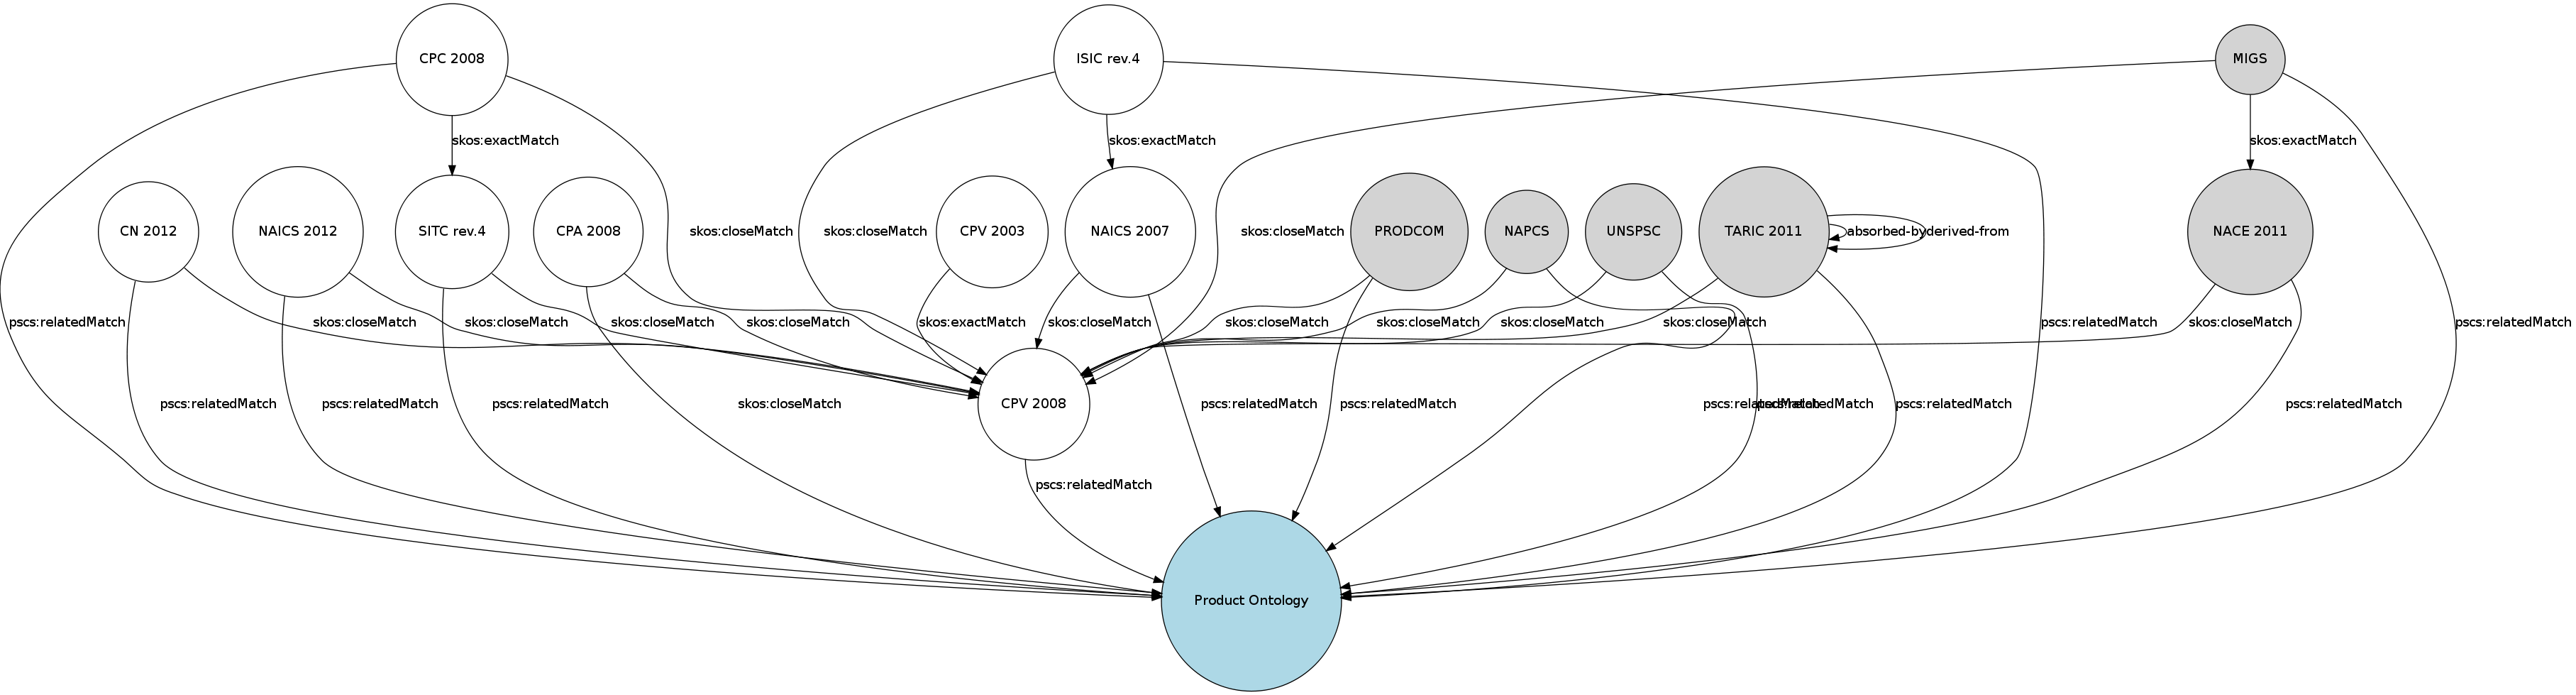
\includegraphics[width=18cm,angle=90]{./images/phd/pscs}
% \caption{Tarea $t_9$-Transformación de los Datos a RDF de las Organizaciones.}
% \label{fig:t9-orgs}
% \end{figure}

\subsubsection{Tarea $t_{10}$-Reconciliación de Entidades}
El diseño y ejecución de esta tarea ha sido descrito en la Sección~\ref{t8-orgs} ya que están 
estrechamente ligadas.

\subsubsection{Tarea $t_{16}$-Añadir metainformación a los recursos RDF}\label{t16-orgs}
Al igual que con las clasificaciones de productos, la metainformación cobra sentido a 
nivel de \dataset, ver Figuras~\ref{fig:orgs-ds},~\ref{fig:people-ds} y~\ref{fig:countries-ds}, ya que no se consideran cambios probables en un corto espacio de tiempo 
en cada una de las entidades gestionadas. En cualquier caso, tratándose de las organizaciones 
la ontología seleccionada para representar el modelo formal de los recursos ya recoge 
la posibilidad de añadir metainformación relativa a posibles eventos de cambios. Teniendo 
en cuenta que la información de las personas está asociada indisolublemente a las organizaciones, tampoco se considera necesario incluir un exceso de metainformación 
en cada uno de estos recursos. Finalmente y en el caso particular de los países, los cambios que se puedan 
producir constituirían una evolución real del \dataset para verificar que la información de todos los países 
sigue siendo congruente. Por ello, se ha seguido el modelo de incluir la metainformación a nivel de 
\dataset y no de recurso en particular. Continuando con los vocabularios seleccionados en los anteriores 
apartados, la especificación realizada por \gls{voID} cubre las necesidades de metainformación para representar 
datos de procedencia, licencia, etc.

\begin{figure}[!htp]
\begin{lstlisting} 
<http://purl.org/weso/eprocurement/organization/resource/ds>
      a       void:Dataset ;
      rdfs:label "Organizations dataset 2011"@en ;
      dcterms:author 
            <http://www.di.uniovi.es/~labra/labraFoaf.rdf#me> , 
	    <http://www.josemalvarez.es/foaf.rdf#me> ;
      dcterms:contributor
            <http://purl.org/weso/pscs/resource/10ders> ,
	    <http://rdfohloh.wikier.org/project/moldeas/rdf> ;
      dcterms:description "Dataset of organizations provided in 10ders project" ;
      dcterms:license <http://opendatacommons.org/licenses/by/1.0/> ;
      dcterms:modified "2011-12-10"^^xsd:date ;
      dcterms:publisher <http://www.josemalvarez.es/foaf.rdf#me> ;
      dcterms:source <http://purl.org/weso/pscs/resource/10ders> ;
      dcterms:title "Organizations dataset 2011" ;
      void:dataDump <http://purl.org/weso/eprocurement/organization/organization-10ders.ttl> ;
      void:exampleResource
        <http://purl.org/weso/eprocurement/organization/resource/org1> , 
	<http://purl.org/weso/eprocurement/organization/resource/org2> , 
	<http://purl.org/weso/eprocurement/organization/resource/org3> ;
      void:uriRegexPattern
        "http://purl.org/weso/eprocurement/organization/resource/.+" ;
      void:vocabulary org: , rdfs: , vcard: ;
      foaf:homepage <http://purl.org/weso> .
\end{lstlisting}
	\caption{Descripción del \dataset de Organizaciones.}
	\label{fig:orgs-ds}
\end{figure}
\cleardoublepage
\begin{figure}[!htp]
\begin{lstlisting} 
<http://purl.org/weso/eprocurement/organization/person/resource/ds>
      a       void:Dataset ;
      rdfs:label "People of the Organization"@en ;
      dcterms:author 
            <http://www.di.uniovi.es/~labra/labraFoaf.rdf#me> , 
	    <http://www.josemalvarez.es/foaf.rdf#me> ;
      dcterms:contributor
            <http://purl.org/weso/pscs/resource/10ders> ,
	    <http://rdfohloh.wikier.org/project/moldeas/rdf> ;
      dcterms:description "Dataset of people working on organizations provided in 10ders project" ;
      dcterms:license <http://opendatacommons.org/licenses/by/1.0/> ;
      dcterms:modified "2011-12-10"^^xsd:date ;
      dcterms:publisher <http://www.josemalvarez.es/foaf.rdf#me> ;
      dcterms:source <http://purl.org/weso/pscs/resource/10ders> ;
      dcterms:title "People of the Organization" ;
      void:dataDump <http://purl.org/weso/eprocurement/organization/person/person-organization-10ders.ttl> ;
      void:exampleResource
        <http://purl.org/weso/eprocurement/organization/person/resource/p1> , 
	<http://purl.org/weso/eprocurement/organization/person/resource/p2> , 
	<http://purl.org/weso/eprocurement/organization/person/resource/p3> ;
      void:uriRegexPattern
        "http://purl.org/weso/eprocurement/organization/person/resource/.+" ;
      void:vocabulary foaf: , org: , rdfs: , vcard: ;
      foaf:homepage <http://purl.org/weso> .
\end{lstlisting}
	\caption{Descripción del \dataset de Personas.}
	\label{fig:people-ds}
\end{figure}


\begin{figure}[!htp]
\begin{lstlisting} 
<http://purl.org/weso/eprocurement/country/resource/ds>
      a       void:Dataset ;
      rdfs:label "ISO 3166 Countries"@en ;
      dcterms:author 
            <http://www.di.uniovi.es/~labra/labraFoaf.rdf#me> , 
	    <http://www.josemalvarez.es/foaf.rdf#me> ;
      dcterms:contributor
            <http://purl.org/weso/pscs/resource/10ders> ,
	    <http://rdfohloh.wikier.org/project/moldeas/rdf> ;
      dcterms:description "Dataset of ISO 3166 Countries" ;
      dcterms:license <http://opendatacommons.org/licenses/by/1.0/> ;
      dcterms:modified "2011-12-12"^^xsd:date ;
      dcterms:publisher <http://www.josemalvarez.es/foaf.rdf#me> ;
      dcterms:source <http://purl.org/weso/pscs/resource/10ders> ;
      dcterms:title "ISO 3166 Countries1" ;
      void:dataDump <http://purl.org/weso/eprocurement/country/countries.ttl> ;
      void:exampleResource
        <http://purl.org/weso/eprocurement/country/resource/ES> , 
	<http://purl.org/weso/eprocurement/country/resource/BE> , 
	<http://purl.org/weso/eprocurement/country/resource/IT> ;
      void:uriRegexPattern
        "http://purl.org/weso/eprocurement/country/resource/.+" ;
      void:vocabulary geo: , rdfs: , dbpedia: ;
      foaf:homepage <http://purl.org/weso> .
\end{lstlisting}
	\caption{Descripción del \dataset de Países.}
	\label{fig:countries-ds}
\end{figure}



\subsubsection{Resultado Final y Ejemplos}
El resultado final del proceso de producción de \linkeddata, tras el análisis y ejecución 
de las tareas identificadas y del método de producción seleccionado, genera como resultado tres \datasets correspondientes 
a las entidades organización, persona y país mediante datos enlazados, en los cuales se pueden extraer las siguientes 
estadísticas de producción de datos, así como ejemplos de los recursos generados, ver Tabla~\ref{table:orgs-ejemplos}. Por otra parte, 
el aumento de la expresividad en el momento de realizar consultas se puede observar en la Figura~\ref{fig:orgs-sparql-query} en la 
cual se expresa la siguiente consulta:

\begin{Frame}
\textit{``Dame la forma de contacto de todas las organizaciones que han publicado anuncios de licitación en un determinado país.''}
\end{Frame}


\begin{longtable}[c]{|p{4cm}|p{3.5cm}|p{2cm}|p{2cm}|p{2.5cm}|} 
\hline
  \textbf{Conjunto de datos} & \textbf{Nº de Elementos}  &  \textbf{Ejemplo} &  \textbf{Tripletas} &  \textbf{Enlaces externos}  \\\hline
\endhead
Organizaciones & $50000$  & Figura~\ref{fig:orgs-example}   & $1150020$  & $50000$ (países)   \\ \hline
Personas & $50000$ &  Figura~\ref{fig:people-example}   & $900219$  & $50000$  (países)  \\ \hline
Países & $246$& Figura~\ref{fig:countries-example}      & $1756$  & $1779$ \\ \hline
\multicolumn{5}{|c|}{\textbf{Organizaciones Personas y Países} (total)} \\ \hline
Agregado & $100246$ &  N/A & $2051995$ & $101779$   \\ \hline
\hline
\caption{Estadísticas y Ejemplos de las Organizaciones.}\label{table:orgs-ejemplos}\\    
\end{longtable}

\begin{figure}[!htp]
\begin{lstlisting} 
SELECT DISTINCT * WHERE{
  ?org rdf:type org:FormalOrganization .
  ?org ref-country ?country.
  ?country rdfs:label ?labelCountry.
  FILTER (?country != <http://nuts.psi.enakting.org/id/ES>).  
  ?org org:hasSite ?site .
  ?org org:siteAddress ?vcard.
} LIMIT 100
\end{lstlisting}
	\caption{Ejemplo de consulta en SPARQL sobre los datos de Organizaciones.}
	\label{fig:orgs-sparql-query}
\end{figure}

\begin{figure}[!htp]
\lstinputlisting{examples/e-proc/country.ttl}
	\caption{Ejemplo final de un País.}
	\label{fig:countries-example}
\end{figure}


\begin{figure}[!htp]
\lstinputlisting{examples/e-proc/org.ttl}
	\caption{Ejemplo final de una Organización.}
	\label{fig:orgs-example}
\end{figure}

\begin{figure}[!htp]
	\lstinputlisting{examples/e-proc/person.ttl}
	\caption{Ejemplo final de una Persona.}
	\label{fig:people-example}
\end{figure}

\newpage

\subsubsection{Método de Producción de \linkeddata de Organizaciones}
Siguiendo las directrices señaladas en el análisis y diseño de entidades 
participantes en el modelado de organizaciones y la tabla de decisión~\ref{tabla:produccion}, el método semántico seleccionado 
para realizar la producción de datos enlazados es el $SPM_1$-``Transformación de datos a RDF'', ver Sección~\ref{spm-1}, en el que 
se transforman un conjunto de datos de entrada $\mathcal{G}$ a un \dataset RDF $\mathcal{D}$. Según la definición de método 
semántico de producción, realizada en la Sección~\ref{method-prod-def}, y el estudio de las organizaciones se pueden 
establecer los siguientes conjuntos:

\begin{itemize}
 \item $\mathcal{G}$ es el \dataset de entrada, conjunto de tuplas, conteniendo los datos de cada una de las organizaciones, las personas y los países. 
 \item $\mathcal{M}$ es el conjunto de \textit{mapeos}, ver Tabla~\ref{table:orgs-mappings}, extraídos según el análisis y diseño realizado en las secciones anteriores. Estos 
\textit{mapeos} son directamente expresables en la herramienta de transformación y toman como parámetros el valor de una de las tuplas de entrada (posición $X$) y la propiedad a generar.
 \item \textit{Dataset} \gls{RDF} $\mathcal{D}$ es el \dataset resultado, siguiendo el análisis y diseño realizado en las secciones anteriores y tras la ejecución 
de la tarea propia de transformación de datos.
\end{itemize}

\begin{longtable}[c]{|p{2cm}|p{8cm}|p{4cm}|} 
\hline
  \textbf{$\mathcal{M}$} &  \textbf{Propiedad} & \textbf{Valor} \\\hline
\endhead
 $m_1$ & \texttt{rdf:type} & \gls{URI} \\ \hline
 $m_2$ & \texttt{rdfs:label} & \texttt{xsd:string@lang}  \\ \hline
 $m_3$ & \texttt{org:purpose} & URI \\ \hline
 $m_4$ & \texttt{org:hasSite} & URI \\ \hline
 $m_4$ & \texttt{org:siteAddress} & URI  \\ \hline
 $m_5$ & \texttt{org:memberOf} & URI \\ \hline
 $m_6$ & \texttt{org:basedAt} & URI  \\ \hline
 $m_7$ & \texttt{ref-country} & URI \\ \hline  
 $m_8$ & \texttt{ref-dbpedia} & URI \\ \hline
 $m_9$ & \texttt{located-in}  & URI \\ \hline
 $m_{10}$ & \texttt{short-label}  & \texttt{xsd:string} \\ \hline   
 $m_{11}$ & \texttt{geo:lat}  & \texttt{xsd:double} \\ \hline
 $m_{12}$ & \texttt{geo:long}  & \texttt{xsd:double} \\ \hline   
 $m_{13}$ & \texttt{vcard:*}  & URI (incluyendo más \textit{mapeos} dependiendo de la información) \\ \hline         
\hline
\caption{Conjunto de \textit{mapeos} $\mathcal{M}$ para las Organizaciones.}\label{table:orgs-mappings}\\    
\end{longtable}

\subsection{Proceso de Publicación de \linkeddata de Organizaciones}
Evidentemente, la estrategia definida para todos los \datasets implicados en el proceso de contratación pública 
electrónica es común, por ello el proceso de publicación es homogéneo siguiendo la estructura definida 
en la Sección~\ref{sect:proceso-publicacion-ld}.

\subsubsection{Tarea $t_{14}$-Infraestructura para \linkeddata}
Nuevamente, la estrategia definida para todos los \datasets implicados en el proceso de contratación pública 
electrónica es común, por ello la infraestructura utilizada es la misma que la definida 
en la Sección~\ref{infraestructura-comun}.

\subsubsection{Tarea $t_{15}$-Acceso y formato en datos RDF}
De la misma forma que en el apartado anterior, el acceso y formato de datos \gls{RDF} para los datos contenidos y relativos 
a las organizaciones siguen el esquema proporcionado en la Sección~\ref{t15-comun}.

\subsection{Proceso de Consumo de Organizaciones}
El proceso de consumo de datos enlazados, según la definición realizada en la Sección~\ref{sect:proceso-consumo}, consiste en 
la reutilización de los datos enlazados para ser aplicados en la construcción de una nueva aplicación o servicio de valor 
añadido. En general, la reutilización más sencilla consiste en la representación gráfica de los recursos o la simple 
consulta con selección de formato de datos de acuerdo a las características de publicación utilizadas. En el caso 
que nos ocupa y teniendo en cuenta el objetivo de realización de un prototipo experimental de extracción de anuncios 
de licitación como demostrador del consumo de datos enlazados, se ha escogido el método semántico de consumo $SCM_2$-``\textit{Mapeo} a Lenguaje de Programación'', 
cuya descripción está disponible en la Sección~\ref{scm2-consumo}, orientado a obtener una representación de los recursos RDF en un 
lenguaje de programación (en este caso Java) como objetos de negocio. De acuerdo a este objetivo y a la definición del propio método 
es necesario definir:
\begin{itemize}
 \item El \dataset RDF $\mathcal{D}_{pub}$, es el conjunto de datos disponible tras aplicar el método de publicación.
 \item El conjunto $\mathcal{M}^1$, ver Tabla~\ref{table:orgs-consumo}, indica como transformar el \dataset anterior a la representación objetivo, objetos del lenguaje Java.
\end{itemize}

De esta manera, se obtienen una serie de objetos, $\mathcal{D}_{consum}$, con la información y datos necesarios, no se transforman necesariamente todos los datos disponibles en los recursos pertenecientes 
a  $\mathcal{D}_{pub}$, para ser reutilizados como objetos de negocio en un lenguaje de programación. Es conveniente señalar que el acceso a los datos se realiza a través 
de la consulta al \textit{endpoint} de \gls{SPARQL} ejecutando consultas \textit{SELECT} y \textit{DESCRIBE}.

\begin{longtable}[c]{|p{2cm}|p{4.5cm}|p{8cm}|} 
\hline
  \textbf{$\mathcal{M}^1$} &  \textbf{Propiedad} & \textbf{Tipo en Java} \\\hline
\endhead
 $m^1_1$ & URI recurso     		& \texttt{java.lang.String} \\ \hline
 $m^1_2$ & \texttt{rdf:type}      	& \texttt{org.weso.moldeas.to.{OrganizationTO, PersonTO, CountryTO}}\\ \hline
 $m^1_3$ & \texttt{rdfs:label} 		& \texttt{Map<String,String>} (lang, value) \\ \hline
 $m^1_4$ & \texttt{org:purpose} 	& \texttt{List<org.weso.moldeas.to.PurposeTO>} \\ \hline
 $m^1_5$ & \texttt{org:hasSite}    	& \texttt{org.weso.moldeas.to.SiteTO} \\ \hline
 $m^1_6$ & \texttt{org:siteAddres} 	& \texttt{org.weso.moldeas.to.SiteAddressTO}  \\ \hline
 $m^1_7$ & \texttt{org:memberOf} 	& \texttt{org.weso.moldeas.to.OrganizationTO}\\ \hline
 $m^1_8$ & \texttt{org:basedAt} 	& \texttt{org.weso.moldeas.to.SiteTO} \\ \hline
 $m^1_9$ & \texttt{ref-country} 	& \texttt{org.weso.moldeas.to.CountryTO} \\ \hline  
 $m^1_{10}$ & \texttt{ref-dbpedia} & \texttt{org.weso.moldeas.to.CountryTO}   \\ \hline
 $m^1_{11}$ & \texttt{located-in}    & \texttt{List<org.weso.moldeas.to.NUTSTO>} \\ \hline   
 $m^1_{12}$ & \texttt{short-label} & \texttt{java.lang.String}\\ \hline   
 $m^1_{13}$ & \texttt{geo:lat} and  \texttt{geo:long} & \texttt{com.javadocmd.simplelatlng.LatLng} \\ \hline   
 $m^1_{14}$ & \texttt{vcard:*} 		& \texttt{org.weso.moldeas.to.VcardTO} \\ \hline   
\hline
\caption{Conjunto de \textit{mapeos} $\mathcal{M}^1$ de consumo para las Organizaciones.}\label{table:orgs-consumo}\\    
\end{longtable}

\subsection{Proceso de Validación de Organizaciones}
La validación como proceso transversal en cualquier etapa dentro del ciclo de vida de datos 
enlazados debe realizarse con el objetivo de asegurar la calidad de los datos. De acuerdo a la 
definición realizada en la Sección~\ref{sect:validation}, este proceso consiste en la comprobación 
de que los recursos de un \dataset RDF cumplen ciertas características. Siguiendo con la estrategia marcada para 
todos los datos implicados en el proceso de contratación pública electrónica, la descripción completa de la validación de acuerdo 
a todas las características, se reseña en las Tablas de Validación disponibles en el Apéndice~\ref{tablas-validacion-apen}.

\subsubsection{Tarea $t_{12}$-Validación de Recursos RDF}
Al igual que en apartados anteriores, de acuerdo a la estrategia definida y con la definición realizada de esta tarea en la Sección~\ref{lod-t12}, 
se puede asegurar que la transformación de la información correspondiente de las organizaciones a la iniciativa \linkeddata cumple estrictamente los 
siguientes puntos:

\begin{itemize}
 \item Los datos \gls{RDF} son correctos ya que se han utilizado herramientas y \gls{API}s (Google \gls{Refine} y Jena) que aseguran 
la generación correcta de RDF.
 \item El dominio y rango en las propiedades es correcta, ya que se realiza la validación contra el modelo definido.
 \item Se ha establecido metainformación sobre la procedencia a nivel de \dataset.
 \item Todos los recursos transformados siguen la plantilla objetivo RDF.
\end{itemize}

\subsection{Proceso de Realimentación de Organizaciones}
Este proceso, según la definición realizada en la Sección~\ref{proceso-realimentacion}, busca la mejora 
y perfeccionamiento de los datos promocionados a RDF. Esta situación emerge en el momento en el cual 
los datos comienzan a ser reutilizados tanto por aplicaciones o servicios como por individuos. En el caso 
particular de las organizaciones y sus entidades relacionadas (personas y países) no se han llegado 
a reutilizar por terceras partes, por lo que la realimentación ha quedado restringida a la captura 
de fallos por la propia aplicación \gls{MOLDEAS}, tratándose en este caso de una forma de realimentación 
basada en \textit{Usuarios y Aplicaciones} y de carácter \textit{Actualización Ocasional}.





\chapter{\label{capitulo:moldeas}Sistema MOLDEAS} % 50
\section{Introducción}
En el caso objeto de estudio de este documento se ha planteado la aplicación de los principios 
de \linkeddata, para el modelado y explotación de datos e información provenientes de los anuncios de 
licitación públicos. Para ello, tal y como se ha presentado en los anteriores capítulos, se ha definido 
un ciclo de vida de datos enlazados que a través de procesos, métodos y tareas suministra una metodología 
de actuación genérica para proceder en este sentido. Como ejemplo de su validez y aplicación se han utilizado 
los datos de los contratos públicos para ejemplificar los procesos de producción, publicación, consumo, validación y 
actualización, ver Figura~\ref{fig:com}. Aunque ciertas tareas se apoyan en el uso de aplicaciones de terceros como Google Refine o bien 
en la parametrización de bibliotecas ya existentes como Apache Lucene, es necesario suministrar un entorno 
en el cual los resultados de aplicación de las tareas puedan ser procesados para implementar algunas de las ya 
especificadas y así ejemplificar transversalmente el uso de datos enlazados en un determinado dominio. Por ello y 
de acuerdo al análisis y especificación realizado se plantea la necesidad de diseñar los componentes del sistema 
MOLDEAS como paso final para la cobertura en el uso de datos enlazados en el campo de la contratación pública 
electrónica y teniendo presentes los siguientes objetivos:

\begin{itemize}
 \item Facilitar y dar soporte a las tareas del ciclo de vida que no puedan ser desarrolladas completamente 
por herramientas externas.
\item Validar los datos generados por otras herramientas.
\item Enriquecer con procesos \textit{ad-hoc} la información y datos de los anuncios de licitación según el modelo 
y especificación fijado en el Capítulo~\ref{capitulo:metodos-separados}.
\item Implementar un demostrador público de consumo de datos enlazados.
\item Proveer un sistema de búsqueda/recomendación de anuncios de licitación de acuerdo a criterios predefinidos 
por el cliente.
\item Establecer un conjunto de prueba que realice la validación parcial de ciertos procesos apoyándose en tecnología 
pre-existente.
\item Diseñar un sistema extensible y escalable para su futura ampliación.
\end{itemize}

\begin{figure}[h]
\centering
\begin{tikzpicture}
  \path[mindmap,concept color=gray,text=white]
    node[concept] {MOLDEAS}
    [clockwise from=0]
    child[concept color=gray!65!black] {
      node[concept] {moldeas-api}   
      [clockwise from=-90]
      child [concept color=gray!60] { node[concept] {\textbf{Consumo}} }   
    }  
    child[concept color=gray!65!black] {
      node[concept] {moldeas-transformer}
      [clockwise from=-90]
      child [concept color=gray!60] { node[concept] {\textbf{Producción}} }
      child [concept color=gray!60] { node[concept] {\textbf{Publicación}} }           
    }
    child[concept color=gray!65!black] { node[concept] {moldeas-test} 
      [clockwise from=-90]
      child  [concept color=gray!60] { node[concept] {\textbf{Validación}} }      
    }
    child[concept color=gray!65!black] { node[concept] {moldeas-common} } ;
   
\end{tikzpicture}
    \caption{Alineación inicial de componentes de MOLDEAS y procesos del Ciclo de Vida de \linkeddata.}
 \label{fig:com}
\end{figure}

Ante estos objetivos de gran envergadura, teniendo en cuenta el ciclo de vida de datos enlazados definido y las tareas 
especificadas para la información y datos presentes en las licitaciones públicas, cabe especificar el diseño 
de los componentes del sistema MOLDEAS como elemento vertebrador tanto de los procesos como de la información. De esta forma, 
a lo largo de este capítulo se realiza una descripción del diseño e implementación realizada en el sistema MOLDEAS haciendo 
especial hincapié en los detalles más relevantes del mismo.
\section{Descripción del Sistema MOLDEAS}
La tarea de análisis de un sistema conlleva la especificación de una serie 
de requisitos que guíen el posterior diseño e implementación del sistema 
\gls{MOLDEAS}. De esta forma, se pueden extraer los siguientes objetivos: 
\begin{itemize}
 \item Analizar e identificar el trabajo relacionado.
 \item Identificar y definir los requisitos asociados a las actividades de investigación, 
innovación y desarrollo a realizar.
 \item Especificar los requisitos de usuario para los distintos componentes
 \item Realimentar los puntos anteriores con los resultados obtenidos.
\end{itemize}

Estos objetivos ya han sido parcialmente cubiertos en los anteriores 
capítulos, en los cuales se ha repasado intensivamente la mayoría de los 
trabajos relacionados y relevantes en el dominio de la contratación 
pública electrónica así como se ha puesto de manifiesto los procesos, 
métodos y tareas a desarrollar dentro del ciclo de vida de datos 
enlazados. Es por ello que este capítulo se centrará en presentar las partes más relevantes y 
destacadas del sistema MOLDEAS y su aplicación en las distintas 
tareas del ciclo de vida así como en el desarrollo del sistema de búsqueda 
de anuncios de licitación. En primer lugar, cabe mostrar un esbozo del 
sistema con una vista funcional del mismo, ver Figura~\ref{fig:functional-overview}, en el cual 
se enclavan los distintos procesos del ciclo de vida y los objetivos generales del sistema: 
producción de datos enlazados de los anuncios de licitación para su posterior 
almacenamiento y publicación a través de un \textit{endpoint} de \gls{SPARQL} y un \linkeddata \textit{frontend} y 
consumo de los datos almacenados para la construcción de servicios de valor añadido como el 
sistema de búsqueda/recomendación de anuncios de licitación. Se ha optado por enfoque 
totalmente práctico en este capítulo de ingeniería con el objetivo de resaltar y documentar la innovación del sistema 
MOLDEAS sin focalizar en metodologías intensivas de ingeniería del \textit{software}.


\begin{figure}[!htb]
\centering
	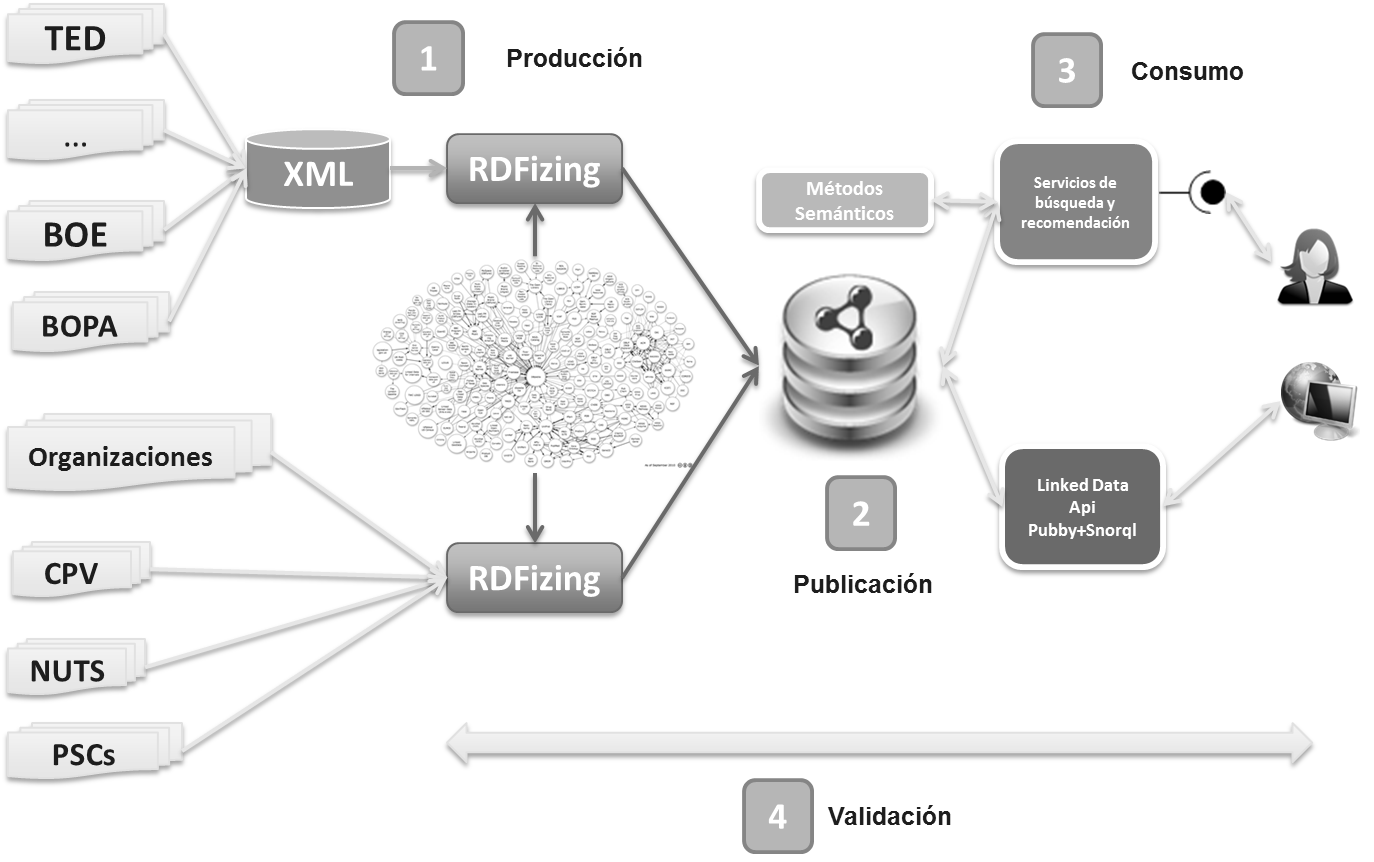
\includegraphics[width=12cm]{images/phd/moldeas/functional-overview}
\caption{Arquitectura funcional del sistema MOLDEAS.}
\label{fig:functional-overview}
\end{figure}

A la vista de la arquitectura funcional propuesta, se ha realizado una aproximación en distintos componentes, 
de acuerdo a sus responsabilidades e interacciones, ver Figura~\ref{fig:moldeas-components}, y con la siguientes 
definiciones:

\begin{description}
 \item [moldeas-common.] Alberga utilidades necesarias a lo largo de todos los procesos del ciclo de vida de datos 
enlazados.
 \item [moldeas-transformer.] Se encarga de dar soporte a la producción de datos enlazados cubriendo las tareas de transformación, 
  enriquecimiento, reconciliación de entidades, etc.  
 \item [moldeas-api.] Se encarga del consumo de los datos enlazados publicados bajo unas 
ciertas características en un \textit{endpoint} de SPARQL y que con la aplicación de varios 
métodos de expansión de consultas es capaz de generar consultas SPARQL cercanas al lenguaje natural 
para la recuperación de los anuncios de licitación.
\item [moldeas-test.] Se encarga de la validación de los datos enlazados y de los métodos de expansión definidos en \texttt{moldeas-api}.
 \item [moldeas-web.] Se encarga de la presentación y consumo de datos enlazados suministrando 
un interfaz gráfico para \texttt{moldeas-api} en el cual el usuario puede seleccionar las 
características de los anuncios de licitación para su posterior búsqueda y 
presentación con diferentes vistas (tabla, mapa, etc.). Además, suministra un interfaz de servicios REST para el acceso 
a los métodos disponibles en \textit{moldeas-api} por lo que cumple una doble función: 1) servir como demostrador 
público para el usuario y 2) ejemplificar las llamadas a \texttt{moldeas-api} desde un punto de vista 
del desarrollador.
\end{description}

\begin{figure}[!htb]
\centering
	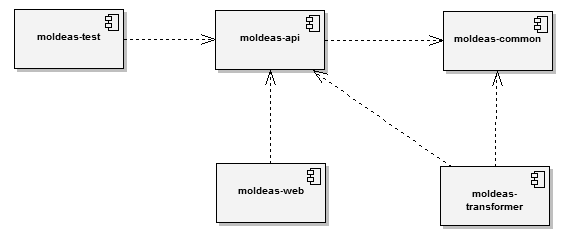
\includegraphics[width=12cm]{images/phd/moldeas/moldeas-componentes}
\caption{Componentes del sistema MOLDEAS.}
\label{fig:moldeas-components}
\end{figure}

\subsection{Arquitectura de alto nivel}
%Diagramas de componentes, diagramas de paquetes
El despliegue de una infraestructura de datos enlazados requiere la cooperación de diferentes elementos 
\textit{hardware} y \textit{software}. Según el análisis realizado de cada uno de los componentes un diagrama 
de despliegue de la arquitectura propuesta en MOLDEAS se presenta en la Figura~\ref{fig:moldeas-despliegue}. 
La descripción de cada uno de estos nodos y componentes es la siguiente:

\begin{itemize}

\item Nodo web. En el cual se encuentran disponibles un servidor web \gls{HTTP} como es Apache2 HTTP Server, este elemento \textit{software} sirve como punto 
de entrada a los elementos del sistema, tanto para el consumo de datos enlazados directamente por otras máquinas como para las peticiones 
relativas al componente \textit{moldeas-web}. También, se utiliza este servicio para albergar una aplicación 
de ejecución de consultas \textit{on-line} en SPARQL como \gls{SNORQL}, sin necesidad de utilizar directamente 
el interfaz propuesto por el \textit{endpoint} de SPARQL.

\item Nodo de aplicaciones web. En el cual se encuentra instalado un contenedor de aplicaciones web \gls{J2EE} como Apache Tomcat, 
con el objetivo de albergar las aplicaciones relativas al \linkeddata \textit{frontend} y a la aplicación \textit{moldeas-web}. 

\item Nodo repositorio RDF. En el cual se instala el repositorio \gls{RDF}, en el cual se almacenan y publican 
los datos enlazados provenientes de los anuncios de licitación. La publicación de datos enlazados se realiza a través de su almacenamiento 
en un repositorio RDF nativo como Virtuoso de OpenLink, suministrando adicionalmente un \textit{endpoint} SPARQL para que los 
datos puedan ser reutilizados y consumidos tanto por la propia aplicación de \textit{moldeas-api} como por clientes 
de forma externa, en este caso se por el \linkeddata \textit{frontend} y SNORQL.

\end{itemize}

Físicamente estos nodos y componentes se han diseñado de forma separada ya que la comunicación entre los mismos 
se realiza mediante delegación de consultas y comunicación mediante HTTP. De esta manera, se permite que el sistema 
sea escalable y flexible, pudiendo sustituir el entorno tecnológico seleccionado por otros proveedores.

Los componentes especificados en MOLDEAS tienen un doble carácter ya que algunos son utilizados de forma \textit{off-line} como 
es el caso de \texttt{moldeas-transformer} y \texttt{moldeas-test}, específicamente para los procesos de producción y validación 
de datos enlazados, mientras que otros como \textit{moldeas-web} sirven como cliente de los servicios proporcionados 
en \texttt{moldeas-api} de forma \texttt{on-line}. Transversalmente \textit{moldeas-common} se utiliza a lo largo de cualquier 
ejecución ya que contiene las clases \textit{Helper} necesarias para la ejecución de tareas comunes.

\begin{figure}[!htb]
\centering
	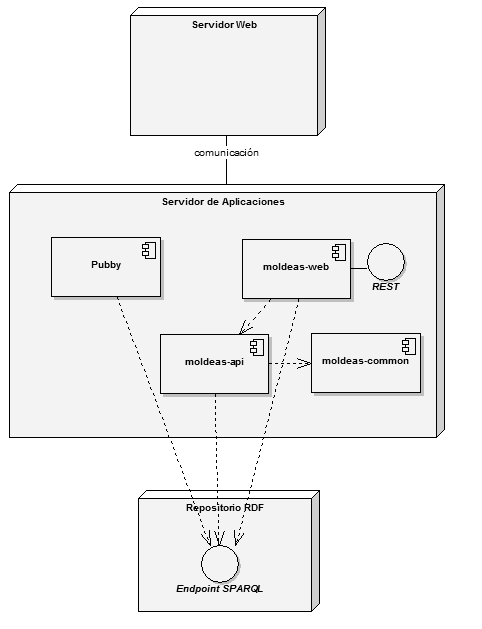
\includegraphics[width=12cm]{images/phd/moldeas/moldeas-despliegue}
\caption{Diagrama de Despliegue de MOLDEAS.}
\label{fig:moldeas-despliegue}
\end{figure}

\subsection{Entorno Tecnológico}
En el momento de analizar y diseñar un conjunto de componentes \textit{software} es necesario seleccionar aquellas 
bibliotecas y herramientas que suministren determinadas funcionalidades de base. La selección estratégica 
de esta tecnología y herramientas se describe someramente a continuación:

\begin{itemize}
 \item Lenguaje de programación Java 1.6. En el campo de la Web Semántica y en particular de la iniciativa de 
datos enlazados, la mayoría de las bibliotecas y funcionalidades externas se encuentran programadas 
en este lenguaje, por lo que unido a la experiencia propia del autor la decisión de uso de este lenguaje 
queda perfectamente justificada.
\item Apache Maven2. El desarrollo de aplicaciones debe realizarse de forma sostenible, es por ello que esta herramienta da 
soporte a todo el proceso de construcción de software: compilación, pruebas, empaquetado, despliegue, documentación, ejecución, etc. 
Además de proveer los mecanismos apropiados para la gestión de dependencias de forma declarativa. 
\item Eclipse \gls{IDE}. La edición del código fuente de las clases Java se ha realizado a través de este entorno de desarrollo, ampliamente 
asentado en la comunidad Java y con una excelente comunidad que proporciona herramientas extra a través de distintos 
\textit{plugins}, proporcionando un entorno productivo y con altas capacidades para el desarrollador. Adicionalmente, Maven 
es capaz de generar a través de su fichero de configuración la estructura de un  proyecto de Eclipse de forma automática.
\item Repositorio de código fuente. Se ha seleccionado la forja de proyectos de Google Code para albergar los cambios y las actualizaciones 
maduras a través del sistema de control de versiones Mercurial.
\item Jena 2.6.4. Biblioteca Java de base tecnológica para la Web Semántica que incluye las principales funciones para el tratamiento de \gls{RDF}, \gls{OWL}, etc. 
así como facilita la ejecución de consultas \gls{SPARQL} tanto de forma local (en memoria) como distribuida (en un \textit{endpoint}).
\item Log4j 1.2.14. Biblioteca Java para la gestión del sistema de registro de una aplicación mediante la cual se puede especificar 
los distintos niveles de registro así como la serialización de los mismos.
\item Junit 4.0. \textit{Framework} Java para la ejecución de pruebas unitarias con un amplio abanico de configuraciones y extras 
para el diseño de pruebas de integración, regresión, etc.
\item Apache \gls{Lucene} 2.9.0. Motor de búsqueda sintáctica en Java con amplias posibilidades tanto para el indexado de documentos, procesamiento 
de lenguaje natural y ejecución de consultas.
\item Apache \gls{Solr} 1.4.1. Plataforma empresarial de búsqueda en Java basada en Apache Lucene que añade nuevas funcionales como nuevos 
filtros para el procesamiento de lenguaje natural.
\item Apache \gls{Mahout} 0.4. Biblioteca Java con un amplio espectro de algoritmos de \textit{data mining} y aprendizaje automático, con capacidades 
para integrarse con otras herramientas como Apache Hadoop y que propone un framework extensible para la creación de nuevos algoritmos.
\item Spring 2.5. \textit{Framework} Java para la creación de aplicaciones empresariales basado en la técnica inversión de control y el uso 
de \textit{Plain Old Java Object} (\gls{POJO}s) para el diseño flexible y el desarrollo ágil de \textit{software}.
\item Jersey \gls{REST} 0.8. Biblioteca Java para la creación de servicios web REST mediante anotaciones.
\item Jquery 1.4.1. \textit{Framework} para el desarrollo de interfaces de usuario enriquecidos basados en HTML+CSS+Javascript.
\item Exhibit 2.2.0. Biblioteca basada en Javascript para el desarrollo de interfaces con múltiples vistas para la presentación 
de datos en general.
\item \gls{Pubby} 0.3.3. \linkeddata \textit{frontend} para la negociación de contenido y presentación de datos enlazados disponibles 
a través de un \textit{endpoint} de \gls{SPARQL}.
\item \gls{SNORQL}. Aplicación basada en HTML+Javascript para la realización de consultas \textit{on-line} sobre \textit{endpoints} de SPARQL.

\end{itemize}




















\section{Consideraciones Generales de Diseño}
En un sentido amplio, dado un problema y un dispositivo en el cual resolverlo, es necesario suministrar un método preciso de respuesta a la casuística 
planteada en el problema de acuerdo al dispositivo objetivo, a tal método se denomina \textit{algoritmo}. El diseño de algoritmos\cite{Vallecillo} 
tiene dos componentes importantes:

\begin{enumerate}
  \item El primero se refiere a la búsqueda de métodos o procedimientos, secuencias
finitas de instrucciones adecuadas al dispositivo del cual se dispone, que permita resolver el problema.  
\item  El segundo permite medir de alguna forma el coste (en tiempo y recursos) de consumo de un algoritmo con el fin de encontrar la
solución, ofreciendo la posibilidad de comparar distintos algoritmos que resuelven un mismo problema.
\end{enumerate}

Una vez que se dispone de un algoritmo que funciona correctamente, es necesario
definir criterios con el objetivo de medir su rendimiento o comportamiento. Estos criterios se centran principalmente en su 
simplicidad y en el uso eficiente de los recursos. La sencillez es una característica sensiblemente interesante en el diseño 
de algoritmos, facilitando su verificación, el estudio de su eficiencia y el mantenimiento. De ahí que muchas veces se priorice la simplicidad y legibilidad 
del código frente a alternativas más crípticas y eficientes del algoritmo. Por otra parte, el uso eficiente de los recursos suele medirse en función de dos
parámetros: el \textit{espacio}, es decir, memoria utilizada, y el \textit{tiempo}, unidades de tiempo de ejecución. En ambos casos, 
se hace referencia a los costes que supone la búsqueda de la solución al problema planteado mediante un algoritmo, además estos dos parámetros 
son utilizados para una posible comparación ulterior de los algoritmos entre sí.

El tiempo de ejecución de un algoritmo dependerá de diversos factores como los datos de entrada que le suministremos, la calidad del código
generado por el compilador para crear el programa objeto, la naturaleza y rapidez de las instrucciones máquina del procesador concreto que ejecute el programa, y la
complejidad intrínseca del algoritmo.  Existen dos tipos posibles de estudio sobre el tiempo:

\begin{enumerate}
\item  Áquel que proporciona una medida teórica (a priori), consistiendo en la obtención de una función que acote 
(inferior o superiormente) el tiempo de ejecución del algoritmo para unos valores de entrada determinados.
\item  El qué ofrece una medida real (a posteriori), consistiendo la medición del tiempo de ejecución del algoritmo para unos valores de entrada determinados 
y un entorno de ejecución particular.
\end{enumerate}

Ambas medidas son importantes puesto que si bien la primera nos ofrece estimaciones
del comportamiento de los algoritmos de forma independiente del ordenador en donde serán implementados y sin necesidad de ejecutarlos, 
la segunda representa las medidas reales del comportamiento del algoritmo. 

\subsection{Consideraciones Diseño de Programas}\label{consideraciones-diseno}
El objetivo de implementación del sistema \gls{MOLDEAS} recae en suministrar parcialmente soporte 
a los distintos procesos implicados en el ciclo de vida de datos enlazados, 
si bien algunas tareas se realizan mediante el uso de ciertas herramientas, existen otras que deben ser parametrizadas e implementadas 
para ofrecer un entorno homogéneo para el manejo de la información y datos 
provenientes de los anuncios de licitación. La separación de responsabilidades 
entre los distintos componentes se realiza de acuerdo a su funcionalidad, de esta manera 
es posible realizar cambios transparentes en los componentes sin que los otros sean 
involucrados en el proceso de cambio: implementación, prueba y empaquetamiento. Por ello, 
se han definido los interfaces de comunicación entre los mismos como un API para que 
cualquier futuro desarrollo se apoye en este \textit{framework} para añadir nuevas 
funcionalidades. Las claves para un diseño abierto de un \gls{API} 
coinciden en muchos sentidos con los de un lenguaje de programación \cite{Interpretes}:

\begin{description}
\item[Concisión notacional:] el API deberá proporcionar un entorno con un nivel
de detalle adecuado: interfaces claras, simples, unificadas etc. Las posibles 
ampliaciones sobre el \textit{framework} de \textit{MOLDEAS} deben resultar sencillas
y no presentar inconvenientes para el programador comprender y extender su diseño.

\item[Ortogonalidad:] la funcionalidad del API debe suministrar el mecanismo
adecuado para combinar nuevos componentes y rechazar algunos de los ya
presentes. Por ejemplo la adición de nuevas restricciones no debe suponer una
recodificación del código del algoritmo.

\item[Abstracción:] el diseño del API debe basarse en el uso de técnicas como
los patrones de diseño e interfaces favoreciendo la abstracción de algoritmos.

\item[Seguridad:] los algoritmos implementados debe tener puntos obligatorios de restricciones
para verificar por ejemplo su terminación aunque se añadan nuevas
restricciones. 

\item[Expresividad:] el API debe ser lo suficientemente ``rica'' como para que
nuevas ampliaciones puedan ser formuladas de forma sencilla de acuerdo a la información 
y datos presentes en los anuncios de licitación y en su modelo formal. 

\item[Extensiblidad:] el API debe basarse en técnicas de programación que
favorezcan la adición de nuevas características y su adaptación para nuevas
configuraciones del algoritmo


\item[Portabilidad:] el lenguaje seleccionado para proporcionar estas técnicas
debe poseer esta característica.

\item[Eficiencia:] en cualquier implementación de un algoritmo o conjunto de los mismos esta característica es fundamental y
aunque el API diseñado, atendiendo a las características anteriores pueda
sobrecargar la ejecución básica de los procesos, su penalización en tiempo no es tan alta 
como para descartar los principios de diseño anteriores.

\item[Librerías e interacción con el exterior:] la ejecución de las funcionalidades 
provistas deberá ser independiente del lenguaje de ontologías utilizado, así aislamos el
conjunto de técnicas de la fuente de conocimiento favoreciendo el uso del
cualquier lenguaje de formalización.

\item[Entorno:] para facilitar la depuración de los algoritmos realizados se
proveerá un entorno gráfico en el cual poder visualizar la ejecución.
\end{description}

Además de estas principios generales para el diseño del API, hay que tener en
cuenta: 

\begin{itemize}
  \item El entorno de ejecución puede ser una aplicación web, por lo que, se
  deberá tener en cuenta en el diseño para que pueda fácilmente integrarse con
  \textit{frameworks} como Spring.
  \item La mayoría de las aplicaciones utilizando Web Semántica utilizan el
  lenguaje Java, por lo tanto, este será el lenguaje seleccionado en su última versión.
\end{itemize}
 
\subsection{Patrones de Diseño}\label{patrones}
Con el objetivo de cumplir los criterios antes mencionadas, el sistema \gls{MOLDEAS} se basará en la aplicación 
intensiva de patrones de diseño\cite{Gamma,CoreJ2EEPatterns} como buena práctica 
de programación. Normalmente estos patrones indican la interacción que ha de realizarse entre los distintos elementos 
que participan en el problema. De esta manera para cada problema tendremos un 
conjunto de objetos, cada uno de los cuales realizará una función proveyendo servicios a 
los demás objetos implicados. Los patrones de diseño proponen soluciones con distintas características: 
elegantes, modulares, escalables y flexibles. Una posible definición de los mismos 
se presenta a continuación:

\begin{Frame}
Los patrones de diseño representan soluciones para problemas recurrentes en la ingeniería del \textit{software}.
\end{Frame}

En general, se trata de soluciones estándar para un problema habitual en programación que utiliza 
distintas técnicas para la flexibilización del código intentando al mismo tiempo satisfacer 
ciertos criterios no funcionales. Se suelen asimilar a una estructura determinada de implementación 
que cumple una finalidad determinada y permite describir ciertos aspectos de un programa.

No obstante, pese a que los patrones nos ofrecen buenas soluciones puede darse el caso de que 
resulte contraproducente el uso de los mismos. El uso de estas técnicas debe realizarse, 
por tanto, en el momento justo. La problemática reside en establecer cuándo su aplicación 
es adecuada y se pueden citar varios criterios:
\begin{itemize}
    \item El código del programa ha crecido exponencialmente.
    \item Las clases de un programa aglutinan código semánticamente no corresponde con su funcionalidad.
    \item Se deben realizar pruebas unitarias de clases.
    \item El diseño del programa es altamente complejo y las relaciones entre las distintas 
clases es opaca.
   \item La comunicación con otros desarrolladores ha decaído debido a la complejidad del código.
\end{itemize}

El libro \textit{The Ganf of Four(Gof)}~\cite{Gamma} fue el pionero en introducir estas técnicas de 
programación caracterizando las mimas en tres niveles:
\begin{description}
    \item [Patrones creacionales:]se utilizan para la creación, inicialización
    Podemos destacar: \textit{Abstract Factory}, \textit{Builder}, \textit{Factory Method}, \textit{Prototype} o
    \textit{Singleton}.
    \item [Patrones estructurales:]su objetivo es separar la interfaz de
    operaciones de la implementación. Tratan de organizar cómo las clases y
    objetos se agrupan para generar estructuras y organizaciones más grandes.
    Por ejemplo: \textit{Adapter}, \textit{Bridge}, \textit{Composite}, \textit{Decorator} o \textit{Facade}.
    \item [Patrones de comportamiento:] describen la comunicación entre los
    objetos.  \textit{Chain of Responsability}, \textit{Command}, \textit{State}, \textit{Strategy} o \textit{Visitor} son
    ejemplos de este conjunto.
\end{description}

En combinación con los patrones de diseño, se encuentra la técnica de \textit{refactoring}~\cite{Fowler1999}, 
utilizada para reestructurar y refinar el código fuente (en muchos casos aplicando un determinado patrón) 
sin alterar la funcionalidad o comportamiento externo del mismo.




\section{Diseño de Componentes del Sistema MOLDEAS}
\subsection{Diseño de \texttt{moldeas-common}}\label{sect:moldeas-common}
El objetivo de este módulo es aunar aquella funcionalidad y lógica 
de negocio común a todos los procesos del ciclo de vida. De esta forma y 
atendiendo al modelo de construcción de aplicaciones Java propuesto 
por Maven se pueden separar responsabilidades entre los distintos 
componentes, compilar y empaquetar (como fichero \gls{JAR}) por separado las distintas clases 
de Java de manera transparente.

Entre las funcionalidades entregadas en este paquete hay que destacar 
las siguientes:
\begin{itemize}
 \item Clases para la carga de ontologías y de documentos RDF desde distintas 
fuentes de datos como ficheros o un \textit{endpoint} de \gls{SPARQL}. 

El doble objetivo de diseño de estos paquetes es: 1) independizar la ejecución de los procesos de la base de conocimiento 
y 2) abstraer la localización  (local, remoto, base de datos, etc.) y contenido del recurso.

Para diseñar estos dos objetivos se han seguido los siguientes criterios:
\begin{enumerate}
  \item El patrón \textit{\gls{DAO}} que sirve como guía para este primer objetivo, abstrayendo
  las operaciones necesarias sobre la base de conocimiento a un interfaz que
  pueda ser implementado por distintos proveedores.
  \item El segundo objetivo, se obtiene factorizando la
  información invariante de los recursos: el contenido del recurso puede ser siempre un
  \textit{InputStream} y todo recurso podrá ser localizado por un identificador
  único (nombre fichero, \gls{URL} o un id. de una base datos), no obstante para
  facilitar la abstracción de la clave de un recurso se ha diseñado como un
  objeto (\textit{KnowledgeResourcePK}) anticipando la necesidad de claves más
  complejas que una simple cadena identificativa. 
\end{enumerate}

En la Figura \ref{fig:moldeas-loading}, se realiza un diagrama de clases del módulo de acceso
a la base de conocimiento.

\begin{figure}[!htb]
\centering
	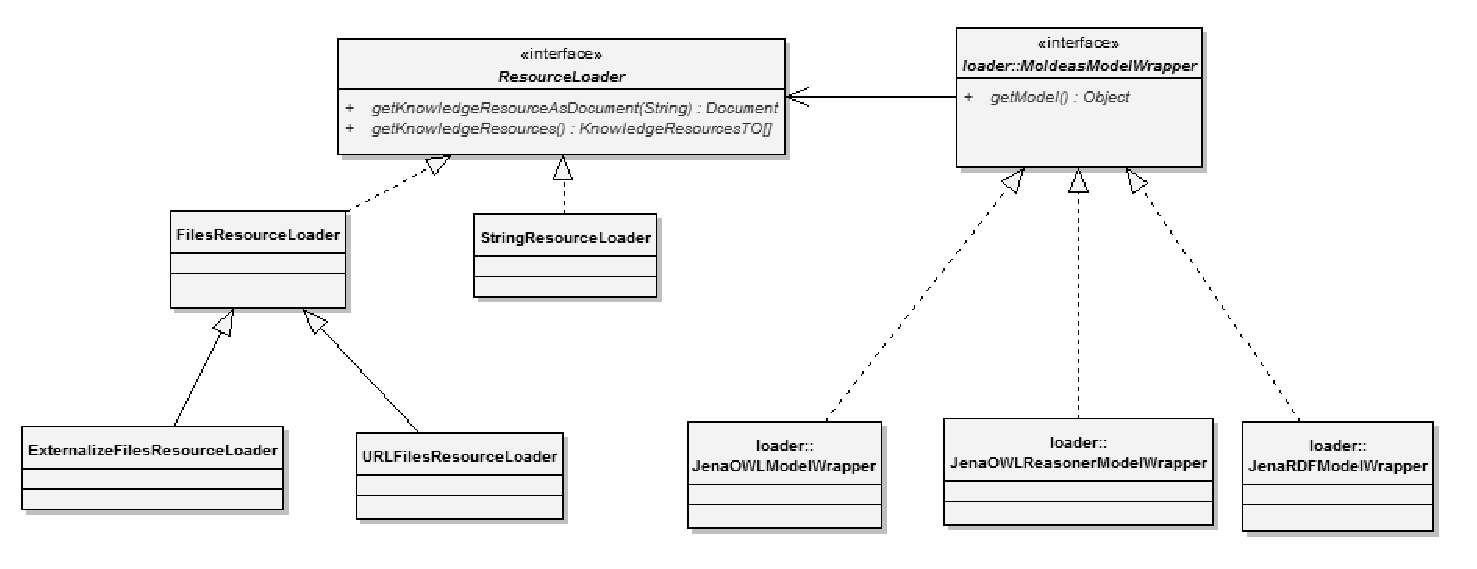
\includegraphics[width=16cm]{images/phd/moldeas/moldeas-loading}
\caption{Diagrama de Clases del acceso a datos (ontologías y RDF) en MOLDEAS.}
\label{fig:moldeas-loading}
\end{figure}


Uno de los puntos clave para facilitar un soporte escalable a los distintos lenguajes, 
consiste en la selección del \gls{API} para trabajar con ontologías y recursos RDF, para ello y teniendo 
en cuenta el uso del lenguaje de ontologías OWL y su representación bajo el modelo 
de datos RDF en sus distintos formatos, se debe realizar una abstracción que permita procesar 
la información y los datos con comodidad, ocultando los detalles de representación sintáctica 
y ofreciendo las abstracciones básicas de \gls{OWL} y \gls{RDF}: sentencias, sujeto, recurso, clases, 
propiedades, etc. En este sentido, las alternativas disponibles se centran en:

 \begin{description}    
  \item[Jena:] biblioteca Java de referencia para el trabajo en el 
campo de la Web Semántica conteniendo múltiples funcionalidades para el desarrollo 
de aplicaciones basadas en RDF y OWL. Se trata de \textit{software libre} 
inicialmente desarrollado por \textit{HPLabs} y actualmente bajo la fundación Apache.

\item[OWL-API:] es una biblioteca para Java específicamente diseñada para tratar ontologías expresadas en OWL. 
Se distribuye bajo licencia de \textit{software} libre y ha sido creada como parte del proyecto europeo 
\textit{WonderWeb}, en la actualidad es gestionada en la Universidad de Manchester. 

\item [Protégé-OWL-API:] utilizada en el IDE Protégé para el desarrollo de ontologías en OWL. Combina aspectos
 tanto de OWL-API como de Jena, no obstante, su ámbito está más orientado hacia a este editor que como biblioteca 
para un usuario programador.         
\end{description}

Una vez valoradas las posibilidades de estas herramientas, se ha seleccionado Jena ya que proporciona soporte 
para el tratamiento de varios lenguajes y formatos de modelado, permite la integración con herramientas 
y procesos externos como los razonadores, y además su comunidad ha crecido exponencialmente 
en los últimos tiempos gracias a su adhesión al proyecto Apache, lo que le confiere un grado 
de madurez y confianza extra que asegura un correcto funcionamiento de la misma.


\item Clases para el almacenamiento de constantes a lo largo del ciclo de vida 
de los datos manejados por el sistema \gls{MOLDEAS}. En este sentido, es conveniente parametrizar 
los valores de las \gls{URI}s base, los grafos RDF, así como los prefijos y espacios de nombres 
de todos los vocabularios y \datasets reutilizados. Esta práctica evita los errores 
ortográficos en la codificación de URIs tanto en la producción de datos como en su consumo 
a través de consultas SPARQL o mediante el propio API definido por Jena.


\item Clases para la gestión de errores y excepciones que se puedan producir a lo largo de cada uno de los procesos 
del ciclo de vida. El diseño de la gestión de errores es uno de los elementos importantes para la
robustez de un producto \textit{software}. Las directrices que se han seguido en MOLDEAS 
para el control de errores es el uso de las excepciones, para ello, se ha creado 
una simple jerarquía de excepciones que capture los posibles errores dentro de la aplicación. 
Se han considerado dos tipos de excepciones, ver Figura~\ref{fig:diagramas/excepciones}:
\begin{description}
\item[Excepciones no chequeadas:]  controlan errores graves producidos en tiempo
de ejecución e inesperados en el modelo. 
\item[Excepciones chequeadas:] controlan errores graves que se pueden producir
en tiempo de ejecución. 
\end{description}


\begin{figure}[htb]
\centering
	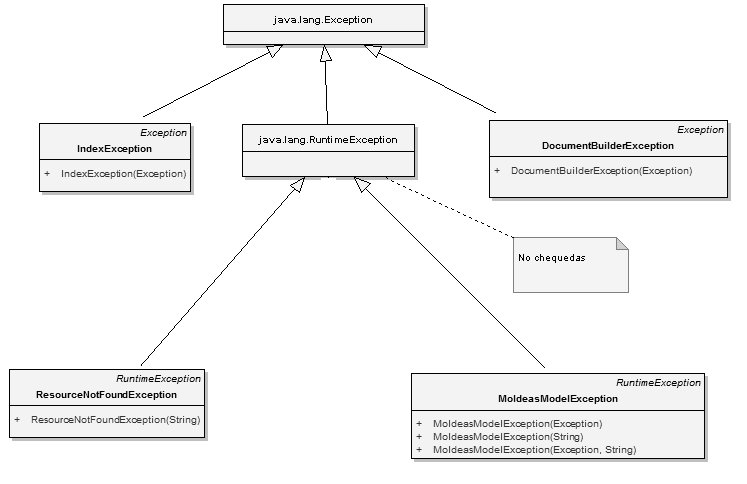
\includegraphics[width=16cm]{images/phd/moldeas/excepciones}
\caption{Diagrama Clases de excepciones en el sistema MOLDEAS.}
\label{fig:diagramas/excepciones}
\end{figure}

\item Clase para la configuración del registro y traza de la aplicación. Esta característica de verdadero valor para una aplicación, 
permite agilizar los procesos de depuración y su integración en sistemas de mayor calado. En todas las clases del sistema MOLDEAS candidatas a 
generar mensajes de registro, se ha utilizado la biblioteca \textit{Log4j} para la gestión del registro de la aplicación. Se trata de una herramienta 
Java para la gestión del registro y traza de acuerdo a un serie de 
niveles: \textit{DEBUG, INFO, WARN, ERROR y FATAL}. Esta división por niveles 
permite configurar los mensajes del sistema dependiendo del estado 
en el que se encuentre: desarrollo, depuración, producción, etc.

\item Otras clases de utilidad para acciones transversales como la carga de documentos 
\gls{XML}, ejecución de consultas \gls{SPARQL}, filtros de lenguaje natural para las bibliotecas 
de Apache \gls{Lucene} y \gls{Solr}.

\end{itemize}

\subsection{Diseño de \texttt{moldeas-transformer}}\label{sect:moldeas-transformer}
El objetivo de este módulo es facilitar el soporte al proceso específico 
de producción de datos enlazados para las distintas entidades de información 
provenientes de los anuncios de licitación. En el enfoque de este trabajo 
se han tenido en cuenta los datos a transformar y promocionar a la iniciativa 
de \linkeddata para agilizar las distintas tareas del modelo de ciclo 
de vida de datos enlazados propuestos. Existen ciertas tareas 
que se pueden acometer directamente con las herramientas existentes como 
Google \gls{Refine}, para las que su funcionamiento es correcto cuando 
los datos son homogéneos y tan sólo requieren la ejecución de una serie 
de \textit{mapeos} o reglas de transformación para utilizar los datos 
de entrada como valores en las tripletas \gls{RDF} a generar. Sin embargo, 
dependiendo del tamaño del \dataset de entrada a transformar, de la homogeneidad 
del mismo y de las operaciones posteriores a realizar como la adición de metainformación, 
la reconciliación de entidades o la simple serialización del modelo RDF en distintos 
formatos, hace necesario la implementación de un proceso personalizado que ejecute 
estas tareas de forma específica, ya que la dificultad de expresarlas en las herramientas 
de propósito general las convierte en tremendamente complicadas. Es por ello, que se han diseñado 
e implementado en este módulo una serie de funcionalidades de carácter específico 
para cada una de las entidades a transformar, teniendo presentes las características 
de las mismas. Para ello, se han considerado los siguientes puntos:

\begin{itemize}
 \item La transformación de la información propia de los anuncios de licitación conlleva la promoción 
de una gran cantidad de datos, que pueden ser tomados de distintas fuentes 
como fichero \gls{CSV}, MSExcel, \gls{XML} o desde una base de datos. En este sentido, 
y debido a dos variables importantes, el tamaño del \dataset y la diversidad 
de los formatos de entrada, se ha optado por la implementación de una serie de adaptadores 
que permiten procesar la información de entrada de forma homogénea de modo que la generación 
en RDF se convierte en un proceso transparente de la fuente de datos y se puede asegurar 
la validez de los datos transformados. En cuanto a la reconciliación de entidades, para este 
conjunto de datos no se considera necesaria ya que se realiza específicamente en el catálogo 
de clasificaciones de productos, sin embargo el enriquecimiento del \dataset de entrada si 
se ve afectado, ya que se han añadido nuevas propiedades (latitud y longitud) a los códigos NUTS para facilitar 
posteriores procesos como el de búsqueda de anuncios de licitación. 

Por tanto, los anuncios de licitación se transforman mediante un proceso Java \textit{ad-hoc} que cubre 
todas las tareas del ciclo de vida referentes a la producción de datos enlazados.

\item En cuanto al catálogo de clasificaciones y teniendo en cuenta las características de las mismas, 
tamaño relativamente pequeño y formato de entrada homogéneo, se ha optado por un enfoque híbrido, en el cual 
en el primer paso se realiza la transformación de los datos originales mediante la herramienta Google 
Refine de forma que una vez obtenidos los datos en RDF se realiza una serie de pasos específicos para la 
reconciliación de entidades (enlazado de las distintas clasificaciones con el CPV 2008) y la adición 
de metainformación. Para ello, se ha implementado un proceso Java capaz de tomar como fuente de datos 
RDF e ir accediendo y enriqueciendo cada una de las descripciones de productos y servicios disponibles, 
basándose en la construcción de un reconciliador de entidades específico con las bibliotecas de 
Apache \textit{Lucene} y \textit{Solr}.


\item Por último y en los datos particulares de organizaciones, países y personas se ha utilizado 
de nuevo un enfoque híbrido en el cual para la transformación inicial se ha optado por la herramienta 
de Google Refine, enriqueciendo y añadiendo a los datos RDF ya generados, las tripletas de información 
necesarias para cumplir con la especificación de recursos RDF realizada.

\end{itemize}

En general, este módulo consta de una serie de procesos independientes que son capaces, para cada una 
de las grandes entidades de información provenientes de los anuncios de licitación pública, de procesar 
los datos en distintos formatos, realizar el proceso de reconciliación de entidades y enriquecer los 
\datasets de entrada mediante la adición de metainformación. 


\subsection{Diseño de \texttt{moldeas-api}}\label{sect:moldeas-api}
Atendiendo a las consideraciones generales sobre diseño, se explicarán 
las decisiones de diseño más relevantes para la construcción 
de un \gls{API} que provee los métodos necesarios para el consumo de datos 
enlazados provenientes de la información de los anuncios de licitación, 
incluyendo las clasificaciones de productos, países y organizaciones.

Este módulo del sistema \gls{MOLDEAS} se encarga de entregar la funcionalidad 
básica, a través de un fichero \gls{JAR}, para dar soporte a los siguientes servicios:
\begin{itemize}
 \item Consumo de los datos enlazados provenientes de los anuncios de licitación, 
clasificaciones de productos y organizaciones desde un entorno de programación y, 
en este caso, desde el lenguaje Java.
\item Construcción de un sistema de recuperación de información, capaz de generar 
consultas en \gls{SPARQL} para ser ejecutadas en el \textit{endpoint} en el cual se encuentran 
almacenados todos los datos.
\end{itemize}

Para dar soporte a estos dos grandes servicios se han establecido una serie de paquetes, 
ver Figura~\ref{fig:moldeas-api-packages}, en los cuales se realizan las funciones 
necesarias que permiten la ejecución de estos servicios. En este dimensionado por paquetes 
se establecen las siguientes funcionalidades:

\begin{itemize}
 \item El paquete \texttt{dao}, en el que se encuentran las interfaces 
que definen las operaciones necesarias para el acceso a los datos enlazados 
de los anuncios de licitación.

\item El paquete \texttt{impl}, en el que se implementan las interfaces 
anteriores mediante clases que realizan el \textit{mapeo} real 
desde los objetos Java de lógica de negocio, a los datos enlazados 
que se encuentran en un \dataset RDF. En este caso, los datos se cargan a través 
de consultas en SPARQL que se pueden ejecutar contra un modelo RDF en memoria 
o bien remotamente en un \textit{endpoint}. El objetivo de este paquete es proveer 
la carga de objetos Java con los datos enlazados provenientes de los anuncios de licitación, 
por ello para cada una de las entidades identificadas se suministra un interfaz de acceso 
que genera las consultas adecuadas en SPARQL para extraer los datos del \dataset RDF. Este 
paquete conforma por tanto el nivel de acceso primario y básico a los datos enlazados, 
constituyendo la primera capa de lógica y acceso a datos del sistema MOLDEAS. Como ejemplo 
se presenta el acceso a datos para los códigos CPV mediante un diagrama de clases, 
ver Figura~\ref{fig:moldeas-api-dao}.

\begin{figure}[!htb]
\centering
	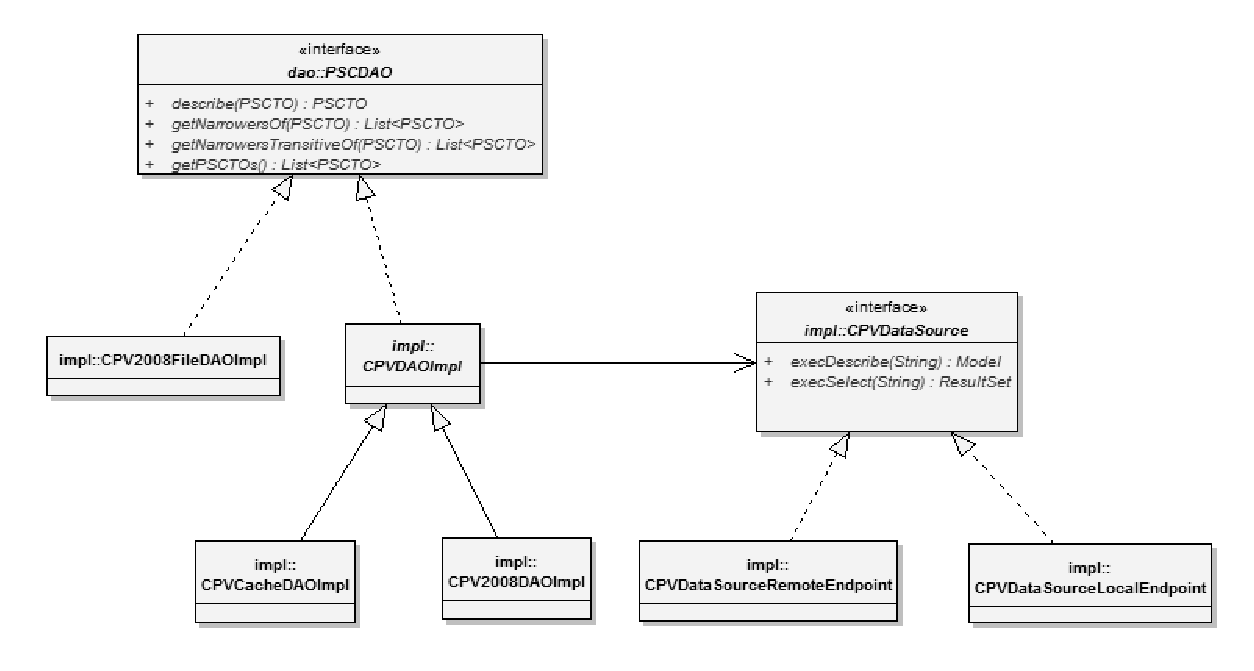
\includegraphics[width=16cm]{images/phd/moldeas/moldeas-dao}
\caption{Diagrama de Clases del acceso a datos (CPV) en \texttt{moldeas-api}.}
\label{fig:moldeas-api-dao}
\end{figure}


\item El paquete \texttt{appserv}, en el que se encuentran las clases con los servicios 
de negocio propios del sistema MOLDEAS, principalmente el servicio de recuperación 
de información y construcción de consultas en SPARQL a partir de un perfil de búsqueda 
del usuario. Adicionalmente, se encuentran clases relativas a la gestión de los objetos 
con la información de los anuncios de licitación.

\item  El paquete \texttt{enhancers}, en el que se establecen las interfaces para la 
expansión de las variables de información correspondientes a un perfil de búsqueda 
de anuncios de licitación. Entre los métodos especificados para realizar la expansión 
de consultas se encuentran aquellos relativos a \textit{Spreading Activation} a través 
de la biblioteca ONTOSPREAD~\cite{ontospreadWSKS11}, los basados en un motor de recomendación como Apache Mahout,
 los basados en un motor de búsqueda sintáctica como Apache Lucene y los relativos 
a las variables numéricas. 

\item El paquete \texttt{psc}, en el que se implementan las interfaces específicas relativas 
a la expansión de la variable de información de los anuncios de licitación correspondiente 
a los códigos de una clasificación de productos, en concreto del CPV 2008. Los métodos aquí 
utilizados son los relativos a la aplicación y configuración de las bibliotecas ONTOSPREAD, 
Apache Mahout, Lucene y Solr.

\item El paquete \texttt{standalone}, en el que se implementan las interfaces específicas 
para otras variables de información secundarias como la información geográfica o la cuantía 
del anuncio de licitación, en este caso de nuevo el principal componente utilizado es la biblioteca 
Apache Mahout configurada a través de distintos ficheros generados mediante el análisis 
del histórico de publicación de anuncios de licitación. Cada una de las implementaciones 
dependiendo de la información que se pretenda manejar debe tomar sus datos de una tabla 
previamente generada en el módulo de \texttt{moldeas-transformer}.

\item El paquete \texttt{ranking}, en el que se específica y se realiza una primera implementación 
de los operadores de agregación para establecer un orden los anuncios de licitación recuperados 
del \dataset RDF, ya sea través de un modelo en memoria o de un \textit{endpoint} de SPARQL. Para cada 
una de las variables de información presentes en los anuncios de licitación se establece una ponderación, cuando 
los anuncios de licitación son recuperados tras el proceso de expansión, se establece una puntuación 
mediante una función lineal que establece un valor según el anuncio extraído contenga más o menos 
elementos de los conjuntos relativos a los códigos \gls{CPV}, \gls{NUTS}, etc.

\item El paquete \texttt{business}, en el que se establece el interfaz de negocio para interactuar con los servicios 
del API, de esta manera se suministra un único punto de acceso como una caja negra, favoreciendo la 
abstracción del número de parámetros y las operaciones.
\end{itemize}

\begin{figure}[!htb]
\centering
	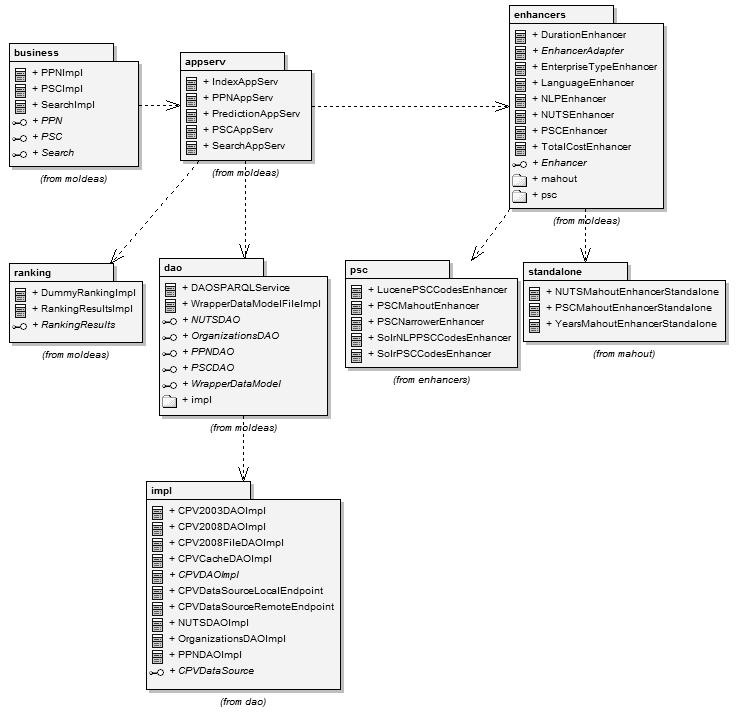
\includegraphics[width=16cm]{images/phd/moldeas/moldeas-api-packages}
\caption{Diagrama de Paquetes relevantes del componente \texttt{moldeas-api}.}
\label{fig:moldeas-api-packages}
\end{figure}

Una vez revisados los principales paquetes de \texttt{moldeas-api}, cabe realizar una descripción 
más completa del sistema de recuperación de información ya que el sistema de expansión de consultas 
se implementa a través de un patrón de diseño denominado \texttt{Chain of Responsibility} en el cual 
a través de distintas iteraciones y modificaciones de la consulta inicial se consigue un perfil 
enriquecido para ser traducido a una consulta en SPARQL. Evidentemente, el objeto contenedor 
del perfil de búsqueda de anuncios de licitación puede ser transformado a cualquier lenguaje de 
consulta tipo SQL o bien a una consulta de un motor de búsqueda sintáctica, esta abstracción 
se consigue de nuevo gracias a un uso correcto de interfaces. En primer lugar cabe especificar 
qué tipo de información y datos contiene un anuncio de licitación que como ya se ha repasado en 
el Capítulo~\ref{capitulo:metodos-separados} y concretamente en la Sección~\ref{sect:rdf-anuncios}, consta 
de una serie de variables de información conteniendo códigos del tipo de licitación, información geográfica, 
metainformación relativa a la cuantía del contrato, el perfil del contrante, la duración, etc. En general, 
y de acuerdo a la información disponible y su tipo se pueden establecer una serie de métodos para realizar la expansión 
de una consulta o perfil de búsqueda.

\begin{itemize}
 \item Información basada en conjuntos y modelada a través de una jerarquía, es el supuesto de los códigos CPV y de la información 
geográfica disponible en NUTS. En este caso los métodos que se pueden aplicar para expandir la consulta son los siguientes:
\begin{enumerate}
 \item Directo. Se navega a través de la jerarquía modelada buscando los elementos más específicos y estableciendo 
un peso determinado para cada uno de ellos. 
 \item Búsqueda Sintáctica. De acuerdo a las descripciones de los códigos se realiza una búsqueda en el \dataset correspondiente, 
buscando no sólo aquellos códigos que encajen perfectamente, sino también aquellos similares, mediante técnicas de procesamiento 
de lenguaje natural.
\item Motor de Recomendación. Realizando un procesamiento previo del histórico de anuncios de licitación y su información, se generan 
una serie de ficheros en los cuales se alinean los códigos CPV con la información relativa a la localización, cuantía o fecha, para que 
de acuerdo a una serie de códigos de entrada se genere una serie de información de salida.
\item \texttt{Spreading Activation}. En este caso se configura esta técnica para que tome un conjunto de conceptos de entrada, en general 
de códigos CPV, para obtener tras la ejecución del algoritmo un conjunto de salida ponderado.
\end{enumerate}

\item Información numérica o asimilable. Se trata el caso de la duración del contrato, la cuantía del mismo, 
el radio de acción geográfico, etc. En este caso los métodos que se pueden aplicar para expandir la consulta son los siguientes:
\begin{enumerate}
\item Basado en el usuario. El perfil de búsqueda del propio usuario define los rangos en los cuales se debe hallar una variable 
numérica sin necesidad de realizar ningún proceso de expansión automático.
\item Uso de lógica borrosa. Se ha valorado el uso de estas técnicas para establecer un intervalo en el cual ponderar 
la pertenencia de un valor a un conjunto. No obstante, en esta primera versión del demostrador público estas técnicas implementadas 
a través de la biblioteca \textit{JFuzzyLogic} tan sólo se han probado y no se han introducido como parte del proceso de 
búsqueda.
\end{enumerate}

\end{itemize}

El objetivo final de estos métodos es obtener para cada una de las variables de información de un perfil 
de anuncio de licitación, una puntuación que permite ejecutar un operador de agregación para así establecer 
un orden entre los anuncios de licitación extraídos tras la generación de la consulta. La importancia de este 
procedimiento por fases reside en que cada uno de los pasos y métodos de expansión se modelan mediante interfaces y 
son ejecutados mediante un proceso iterativo de enriquecimiento, como se puede ver en la Figura~\ref{fig:moldeas-api-search}, 
que permite la adición de nuevos métodos de forma sencilla, simplemente reconfigurando las implementaciones de 
los interfaces a través del fichero de configuración de Spring. El flujo y la comunicación 
entre las distintas clases que intervienen en el proceso de expansión y recuperación de información 
se presenta a través de la Figura~\ref{fig:moldeas-search}, en el cual es preciso señalar 
como las responsabilidades son compartidas a través de los distintos objetos situados en distintas 
capas lógicas.

\begin{figure}[!htb]
\centering
	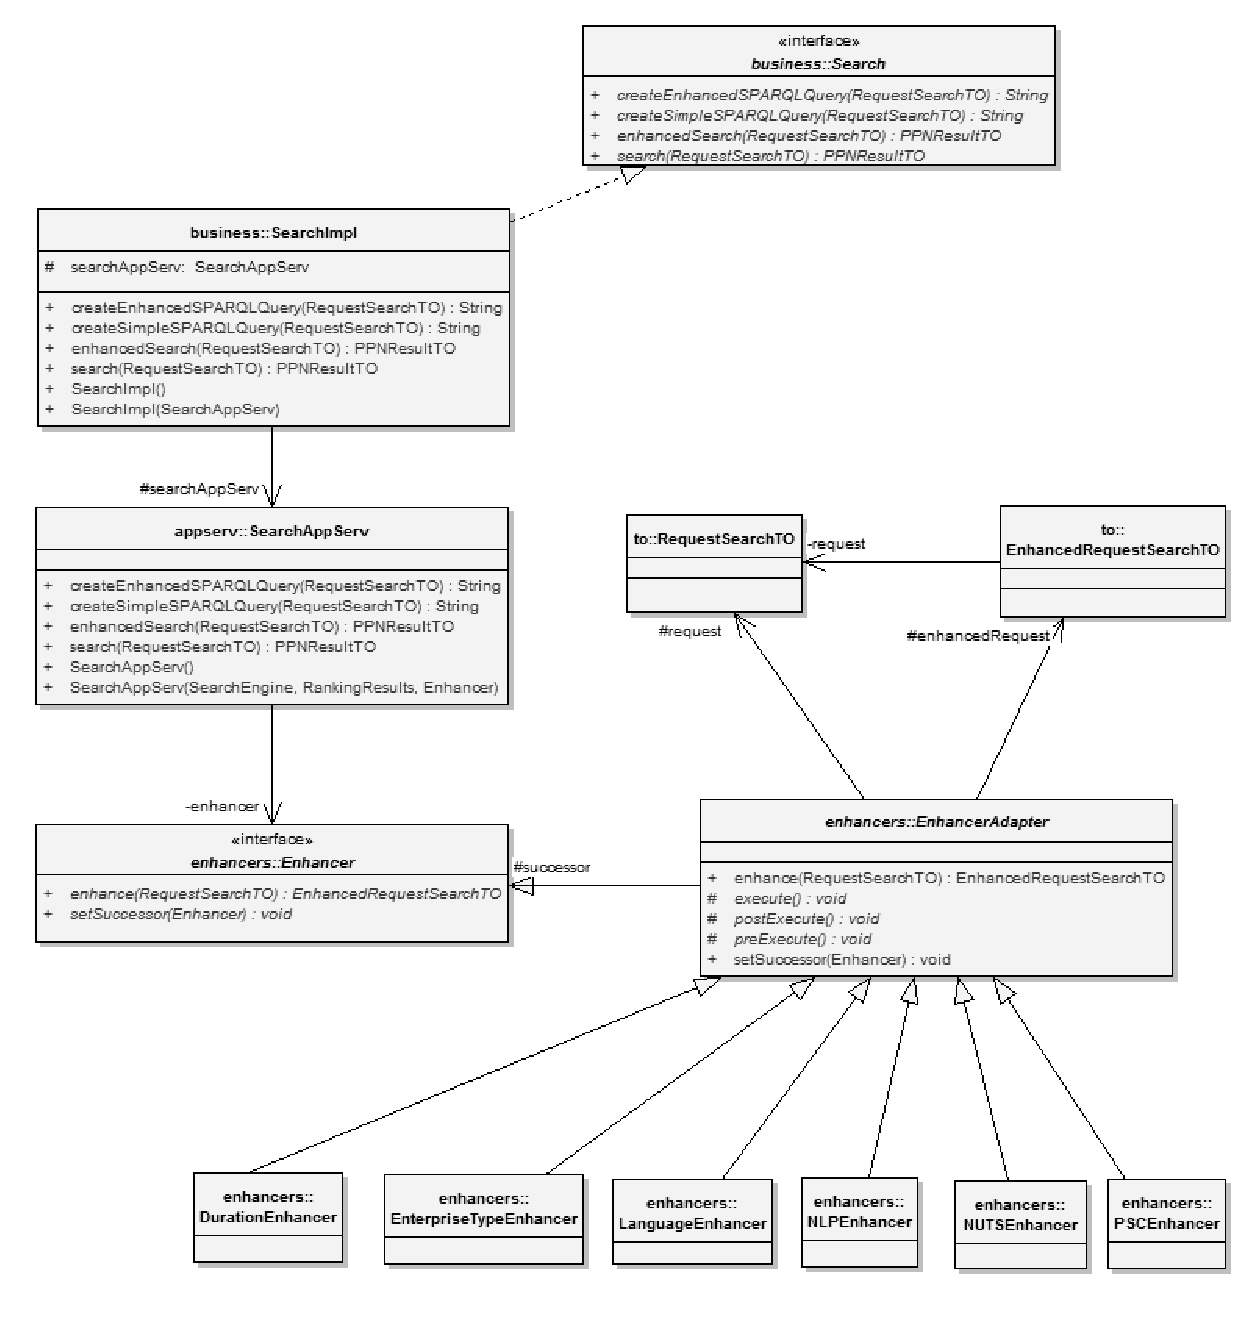
\includegraphics[width=16cm]{images/phd/moldeas/moldeas-chain}
\caption{Diagrama de Clases del sistema de búsqueda en \texttt{moldeas-api}.}
\label{fig:moldeas-api-search}
\end{figure}


\begin{figure}[!htb]
\centering
	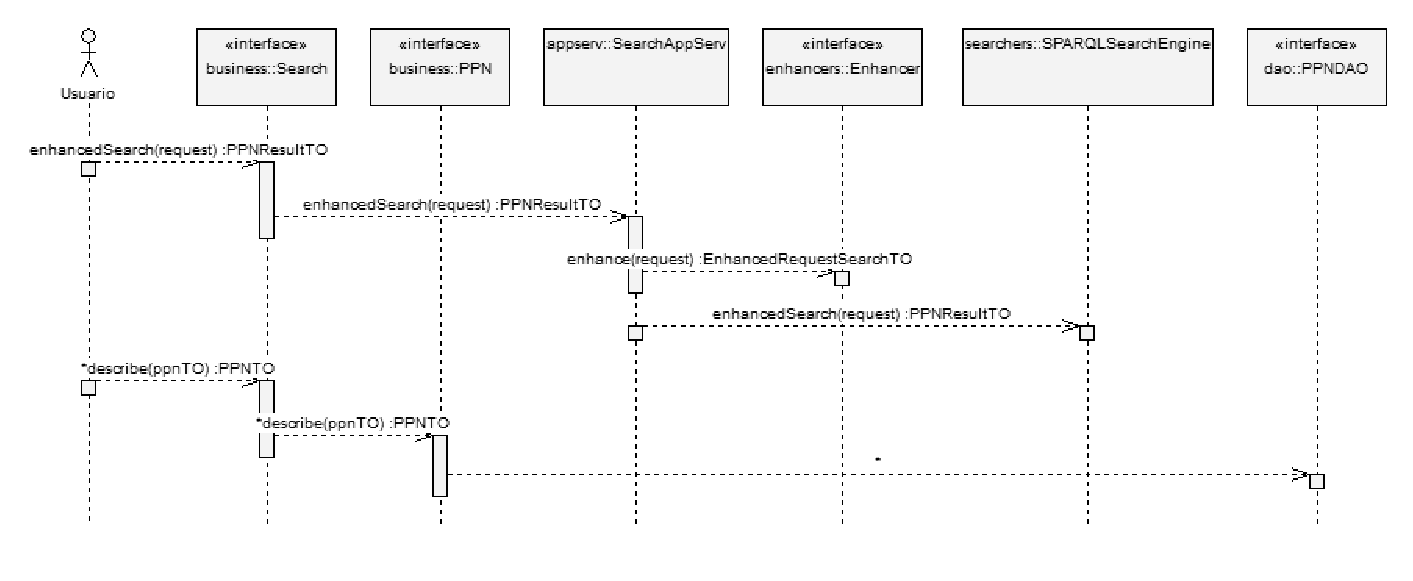
\includegraphics[width=16cm]{images/phd/moldeas/moldeas-search}
\caption{Diagrama de Secuencia de la búsqueda en \texttt{moldeas-api}.}
\label{fig:moldeas-search}
\end{figure}


Finalmente, en este apartado cabe señalar los patrones de diseño, ver Tabla~\ref{tabla:patrones}, que se han aplicado 
para obtener un sistema flexible y escalable en el cual nuevas implementaciones 
de los interfaces sean fácilmente integrables proporcionando un API para el consumo de datos enlazados y recuperación de información de los anuncios de 
licitación.


\begin{table}[htb]
\renewcommand{\arraystretch}{1.3}
\begin{center}
\begin{tabular}{|p{6cm}|p{8cm}|}
\hline
        \multicolumn{2}{|c|}{\textbf{Patrones de Diseño}}\\        
        \hline
        \textbf{Nombre} &  \textbf{Aplicación} \\ \hline       
			\textit{Adapter}&Implementación para el acceso y transformación de los datos de los anuncios de licitación.\\ \hline
			\textit{Chain of Responsibility}&Implantación del sistema de enriquecimiento de consultas.\\ \hline
			\textit{DAO}&Abstracción de acceso a la base de datos y de conocimiento.\\ \hline
			\textit{Template Method}& Implementación por omisión de métodos en el patrón \textit{Chain of Responsibility}.\\ \hline
			\textit{Factory Method}&Creación de objetos provenientes de Spring.\\ \hline
			\textit{Template Method}&Funciones con llamadas a métodos de interfaces, por ejemplo en los \texttt{Enhancers}.\\ \hline
			\textit{Transfer Object}&Comunicación de información entre los distintos módulos y capas.\\\hline 
			\textit{Singleton}&Creación de objetos de acceso a datos, etc., provenientes de Spring.\\ \hline
			\textit{Otros}&Relativos al diseño por capas de aplicaciones J2EE.\\ \hline
		\hline
		\end{tabular}
		\caption{Principales Patrones de Diseño utilizados en MOLDEAS.}
		\label{tabla:patrones}
  \end{center}
\end{table} 

\clearpage
\subsection{Diseño de \texttt{moldeas-test}}\label{sect:moldeas-test}
El objetivo de este módulo es abstraer las pruebas de los módulos anteriores, 
especialmente de \texttt{moldeas-api}, para así proveer un sistema separado 
de ejecución de \textit{tests} en el cual se puedan realizar las siguientes 
acciones:

\begin{itemize}
 \item Creación de configuraciones del \gls{API} de \gls{MOLDEAS} a través de distintos 
ficheros de Spring que permiten probar de forma automática la combinación 
de los distintos métodos de expansión de consultas así como verificar 
sus resultados.
\item Validación de los recursos \gls{RDF} generados de acuerdo a unas reglas de validación 
extraídas de las tablas de validación establecidas en el Apéndice~\ref{tablas-validacion-apen}.
\end{itemize}

De esta manera se ofrece un módulo separado con un doble sentido, para la realización de pruebas de caja negra de los 
servicios disponibles en el API de MOLDEAS, así como para la propia validación de los datos enlazados. La configuración 
de este módulo se realiza a través de un fichero \gls{XML} \textit{ad-hoc} en el cual se cargan las configuraciones 
para ejecutar los \textit{tests} pertinentes (en forma de plantilla) mediante Junit. No obstante, en la Sección~\ref{sect:pruebas-moldeas} se realiza una descripción 
más detallada de las pruebas llevadas a cabo.


\subsection{Diseño de \texttt{moldeas-web}}\label{sect:moldeas-web}
El objetivo principal de diseño de este módulo es definir y diseñar un herramienta de acceso gráfico 
a los servicios del sistema \gls{MOLDEAS}. Es importante destacar que este cliente gráfico se realiza con el objetivo de facilitar 
un demostrador público ya que el uso de la biblioteca de \texttt{moldeas-api} es perfectamente 
válido desde cualquier programa así como desde el interfaz de servicios REST, que también se incluye 
en este módulo. Por tanto, este módulo surge para abarcar las siguientes funcionalidades:

\begin{enumerate}
\item Proveer un interfaz de servicios \gls{REST} que sirva tanto para exponer los 
servicios de negocio, como para ejemplificar las llamadas del \gls{API} de MOLDEAS.

El interfaz de servicios REST diseñado, simplemente añade una capa extra de indirección a los 
servicios de negocio suministrados en el API de MOLDEAS, se duplica la signatura de los métodos 
en una nueva capa simplificando las llamadas. La idea de realizar un interfaz REST surge para dar soporte a la tendencia actual de publicación 
de servicios web \gls{HTTP} y también para ejemplificar las llamadas al API (construcción de parámetros, gestión 
de los resultados, etc.), en cualquier caso, cualquier cliente siempre puede utilizar 
la versión de \texttt{moldeas-api} empaquetada individualmente. Para realizar este API de servicios 
REST se ha utilizado la biblioteca para Java-Jersey \gls{REST} 0.8 y la descripción de los mismos 
se presenta, parcialmente, en la Figura~\ref{fig:moldeas-wadl} en formato \gls{WADL}.


\begin{figure}[!htp]
\lstinputlisting[language=XML,basicstyle=\scriptsize]{examples/moldeas-pretty.wadl}
	\caption{Interfaz REST en formato WADL.}
	\label{fig:moldeas-wadl}
\end{figure}


\item Suministrar un interfaz gráfico que ejemplifique las llamadas a los servicios REST y que a su vez sirva como demostrador público para el acceso a los datos de los anuncios de licitación 
y para la recuperación de información. La construcción de este interfaz se ha desarrollado utilizando 
bibliotecas de Jquery y HTML facilitando la creación de interfaces enriquecidos de programación 
sencilla.

\item Aunar las herramientas externas de publicación y acceso a datos enlazados en un sólo punto de entrada. En este sentido, 
el interfaz web creado también contempla ejemplos de consultas en SPARQL a realizar mediante la herramienta 
\gls{SNORQL} y enlaces a ejemplos de recursos que son consultados a través de un \linkeddata \textit{front-end} como 
Pubby.
\end{enumerate}

\subsubsection{Conceptos y Diseño de la Interacción Gráfica}
En los últimos años, el aumento en el uso de las nuevas tecnologías de la información ha 
conllevado un cambio fundamental en la sociedad que provoca la necesidad de adecuarse a nuevas 
relaciones que se establecen entre la persona y la máquina. Esta necesidad de interacción supone 
que la comunicación entre persona y máquina adquiera una especial relevancia en nuestro tiempo. Se maniesta
 un desafío consistente en proporcionar de significado a los productos y servicios ofrecidos, 
intentando dotarlos de estructura y comprensión cercana a la escala humana.

Debido a la complejidad interna de los ordenadores, la comunicación entre los entes debe realizarse 
a un nivel conceptual, predominando la comunicación visual, gráfica y verbal como medio para llegar 
a la comprensión. La idea subyacente está referida a la necesidad de encontrar el modelo ideal que permita a la persona 
interaccionar con las máquinas como si fueran un humano más.

En esta situación se hace especialmente relevante la generación de interfaces de usuario 
que se adecúen a las necesidades de las personas, por ello las reglas propuestas por 
\textit{Sneiderman} suponen un primer acercamiento a la interacción persona ordenador y una 
métrica para evaluar la bondad de un interfaz de usuario.

En este sentido, desde los anales de la historia los hombres han ideado formas e instrumentos
(lenguajes de símbolos, de texto, gráficos, etc.), tanto para la comunicación de sus experiencias, 
como para reproducir la realidad. La forma de expresión depende en buena medida del ambiente 
tecnológico y de los lenguajes utilizados entre el emisor y el intérprete para decodificar los mensajes. 

La riqueza de expresión de un lenguaje se basa en el principio de concordancia entre los entes 
participantes del acto comunicativo, para que se establezca este acto deben estar en correcta relación. 
Desde el punto de vista de un interfaz gráfico estos factores quedan patentes por la dificultad 
que entraña ofrecer un entorno en el cual tanto: percepción, interpretación y comprensión sean 
lo suficientemente claros para que el ser humano no se sienta en un entorno extraño.

Los seres humanos a través de su sistema nervioso son capaces de percibir 
lo que sucede en su entorno y actuar en consecuencia, puede considerarse que el hombre es una fuente de información, percibe 
y recibe estímulos externos que le permiten adaptar sus respuestas. 

Comprender el comportamiento humano como sistema de comunicación supone una gran dificultad, 
tanto en capacidad para interpretar, como para decodificar los mensajes, haciendo imposible 
conocer su respuesta exacta ante la recepción de un mensaje. El problema de la comunicación entre personas y 
máquinas no consiste en reducir el comportamiento humano al de una máquina, sino analizar 
las necesidades y capacidades para adaptar la presentación de información a su nivel, acercándose 
lo más posible al proceso cognitivo de la persona.

La visión es nuestro medio natural de percepción de los mensajes, limitada por condiciones físicas, 
por ello cobra especial relevancia para la distribución de información en un documento, 
dependiendo la compresión de la persona de la bondad de la misma. No obstante, este modelo a seguir no es 
completamente válido ya que habría que tener en cuenta las necesidades de las personas con discapacidades de distinto tipo, 
intentado adaptar el contenido al sujeto participante de la comunicación.

Utilizando los distintos sentidos de los que disponemos como fuentes de adquisición de información 
debemos ser capaces de procesar y comprender esta información, esta capacidad puede denominarse 
\textit{entendimiento humano}, mediante el que determinamos nuestros actos a partir de las percepciones 
sensoriales. De todos los estímulos percibidos, sólo permanecen aquellos que generan un mayor impacto, 
este será un factor muy relevante en el diseño de un interfaz, por ejemplo cuando se selecciona una combinación de colores.

Debe tenerse en cuenta, que aunque el funcionamiento general humano es similar no puede ser 
predecible, ni aplicable por extensión, se cometería en un grave error de 
interpretación del comportamiento, este punto es especialmente interesante a la hora de adaptar un interfaz 
gráfico a las distintas personas, estableciendo perfiles.

Las 8 reglas de Oro de \textit{Sneiderman} nos ayudan a este objetivo, intentando simplificar 
la comunicación persona-máquina. A continuación, se comentan estas reglas:

\begin{description}
\item[Esforzarse por la consistencia.] Es el principio por el cual los
elementos y relaciones deben ser presentados de forma idéntica e inequívocamente. Este concepto es aplicable a:
\begin{itemize}
\item Tipografía, por ejemplo enfatizar siempre con el mismo estilo.
\item Iconos, la misma acción debe estar representada por el mismo icono.
\item Comandos y menús, la información que se utilice en los menús deberá ser representativa
de su acción interna.
\item Funcionamiento multiplataforma, esta cualidad se pone de manifiesto actualmente, ya que se accede a la misma información utilizando diferentes medios: navegadores, móviles, etc.
\item Percepción del sistema igual para todos los usuarios.
\item Estructura el sistema de forma que se adapten al entorno de trabajo del usuario.
\end{itemize}

Por lo tanto la consistencia nos remite a obtener una representación de los objetos 
coherente en su significado, formas y métodos en el mismo contexto. 
También puede entenderse la consistencia como la relación que se establece entre 
una metáfora de representación y su uso real.

\item[Permitir a los usuarios frecuentes utilizar atajos:] se considera un
usuario frecuente a una persona que interacciona con un interfaz gráfico con soltura, debido 
sobre todo a la experiencia en su uso. Este tipo de usuarios, a medida que avanza su 
manejo del interfaz, se convierten en expertos, exigiendo mayores prestaciones a la aplicación desde distintos puntos de vista: 
1) adaptabilidad y 2) velocidad de ejecución.

Esta característica a tener en cuenta en los interfaces, se aplica no sólo a los usuarios 
expertos sino a la necesidad de que un interfaz sea adaptable a las nuevas necesidades que se 
manifiestan en el usuario a través del uso.

Por otro lado, los atajos deben ser fáciles de recordar y mejorar el rendimiento, por ejemplo 
sería contraproducente un atajo de teclado de cuatro teclas ya que sólo el posicionamiento correcto 
de los dedos sería más penalizador que utilizar un ratón.

\item[Ofrecer retroalimentación informativa.] Debido al concepto de acto
comunicativo, resulta importante que cuando un usuario realiza una acción se vea recompensada con una respuesta del sistema. 
De esta forma, se consigue que se establezca la metáfora de la comunicación entre el 
emisor (usuario) y el receptor (máquina), permitiendo una comunicación fluida.

Este objetivo es relevante en cuestiones relacionadas con el establecimiento del éxito o no de la operación 
realizada por el usuario, por ejemplo si en un navegador no se dispone de conexión a internet 
y se solicita el acceso a una página, el proceso de espera sería tedioso, utilizando una barra de 
progreso de carga se consigue realimentar el estado de la acción solicitada e iniciada por el usuario.

\item[Diseñar diálogos para fundamentar el cierre.] Con esta característica
se consigue acotar el inicio de una secuencia de acciones, fijando
su inicio, desarrollo y final. Respetando este punto se consigue que el usuario se sienta satisfecho, ya que sabe si la acción que ha realizado ha seguido la secuencia correcta, utilizando todos los pasos previstos hasta llegar a un fin.

\item[Ofrecer prevención de errores y manejo de errores simples.] La gestión de
errores es importante en cualquiera de los aspectos dentro de una aplicación informática.
En el contexto de un interfaz de usuario queda patente la necesidad y las ventajas que conlleva 
disponer de un interfaz que minimice los errores, involuntarios o no, provocados por los usuarios.

Un escenario de uso podría ser la introducción de una fecha, generalmente para facilitar 
la interacción con el usuario se genera una máscara de entrada o bien un ejemplo que 
permita al usuario cambiarlo para así facilitar sus tareas.

El objetivo, es que el usuario se preocupe de sus tareas y no del funcionamiento del 
interfaz, es decir, que el manejo del mismo no suponga un trabajo extra.

No obstante, este objetivo no siempre se puede conseguir, de ahí que cuando se produzcan errores 
no críticos de la aplicación, tales como errores en la introducción de 
datos o una secuencia de pasos inválidos para realizar una acción, sería conveniente que el sistema fuera capaz de ofrecer 
un mecanismo tutor para enseñar al usuario al manejo sin errores. 
Un claro ejemplo podría ser el famoso ``ayudante'' de Microsoft Word que si bien realiza su función, en ocasiones llega a resultar molesto.

Los tutores dentro de las aplicaciones para aleccionar a los usuarios, y prevenir errores, 
se deben diseñar con sumo cuidado y acotando muy bien su ámbito de acción ya 
que su efecto puede ser el contrario del pretendido. En estos casos, el menos es más puede 
resultar útil y un simple texto desplegable con un ejemplo puede ser suficiente.


\item[Permitir inversión de las acciones.] Esta característica ofrece la
admirable ventaja de ofrecer confianza al usuario en su diálogo con el interfaz gráfico. 
Suponiendo que un usuario novel realiza una serie de acciones secuenciales y antes de grabar 
los cambios se percata de que ha cometido un fallo, podría pensar en distintos escenarios, así:
\begin{itemize}
\item Tranquilidad, el interfaz permite deshacer cambios, se puede retroceder para corregir lo que se ha realizado de forma incorrecta.
\item Desconsuelo, después de estar X tiempo realizando una tarea se tiene que deshacer debido a un insignificante error, tiempo perdido.
\end{itemize}

Parece claro que el sentimiento de tranquilidad es más deseable en un usuario, así que es 
importante cumplir esta característica.

Desde otro punto de vista, el usuario se sentirá más tranquilo y seguro en el uso del interfaz 
si sabe que tiene más de una oportunidad cuando utiliza las funciones de la aplicación, 
de otra forma un sentimiento de angustia podría invadirle produciendo errores en el usuario y 
empeorando su rendimiento en el uso de la aplicación.

El sentido de estos cambios debería ser tanto hacia adelante como hacia atrás, ya que sino se desaprovecha 
la potencia de esta propiedad.

\item[Apoyar el control de los usuarios:] en la tarea de satisfacer al usuario,
éste debe percibir que el sistema está ejecutándose bajo su supervisión y respondiendo a sus acciones. 
Todo aquello que sea público al usuario deberá permitir su control, siempre dentro de unos límites, 
ya que de otra forma quizás se obtuviera un sentimiento de insatisfacción.

Debería evitarse por ejemplo introducción de datos tediosa, comportamiento extraño de la aplicación 
(acciones o comandos que no funcionan o no responden) o imposibilidad de obtener información 
(sabemos que se ha introducido pero se desconoce cómo acceder a ello).

\item[Reducir la carga de la memoria a corto plazo:] esta necesidad surge por
una limitación en la memoria humana para procesar información a corto plazo, por ello, cuando 
un interfaz emita mensajes al usuario deberán ser cortos de modo que pueda comprender 
rápidamente la información que se envía desde la máquina.

También es conveniente no tener demasiadas ventanas abiertas dentro de un entorno, 
ya que pueden despistar al usuario y no saber dónde está exactamente.

\end{description}

El diseño de un interfaz gráfico para el sistema MOLDEAS es una tarea relativamente
sencilla, ya que el problema real consiste en suministrar un interfaz habitual 
al usuario en el cual pueda seleccionar las características de su perfil 
de búsqueda. En cualquier caso, se optado por un interfaz gráfico 
lo más sencillo, intuitivo, consistente y uniforme posible.









\section{Pruebas del Sistema MOLDEAS}\label{sect:pruebas-moldeas}
La metodología de la Programación Extrema~\cite{XP} (\gls{XP}), que ha servido de guía para el desarrollo 
del sistema MOLDEAS, hace hincapié en la importancia de las pruebas. La realización de ciclos de desarrollo breves
(incorporando la funcionalidad perseguida en pequeñas versiones totalmente funcionales) habilita la posibilidad de 
concentrarse en la validación, en cada momento, de un segmento reducido del código o de la funcionalidad, 
dependiendo del nivel de la prueba. Pero también exige la existencia de un mecanismo que permita 
realizar los ensayos de forma automática; de lo contrario, la obligación de repetirlos 
frecuentemente los convertiría en extremadamente tediosos.

\subsection{Pruebas Caja Blanca}
Son pruebas que se realizan para verificar la validez de las operaciones internas del programa, 
intentando garantizar que todos los caminos de ejecución del programa han sido probados. Para realizar las pruebas de caja blanca se han 
seleccionado las pruebas unitarias por su importancia dentro la metodología de Programación Extrema. 
La descripción de las pruebas unitarias se amplia a través de los siguientes puntos.

\begin{description}

\item [Validación con pruebas unitarias:] representan el nivel más bajo de prueba del \textit{software}, 
permitiendo al desarrollador obtener retroalimentación instántanea del correcto
comportamiento (o no) de un componente determinado.

\item [Necesidad de las pruebas unitarias:] como buena práctica de programación
el desarrollador debería codificar la prueba antes que la propia funcionalidad,
para así pensar los resultados antes de obtenerlos. Como norma general, un buen
test siempre debería fallar la primera vez. Por otra parte, facilitan la
depuración, si un test falla tenemos un ámbito muy reducido en el cual localizar
el error, se incrementa la productividad de los desarrolladores. 

Además, desde el punto de vista de la gestión de un proyecto un buen conjunto de
pruebas unitarias se pueden utilizar como documentación del código fuente, así,
por ejemplo si se introducen nuevos desarrolladores éstos pueden comprender
fácilmente la funcionalidad que se está realizando y probando.

\item [Codificación de Pruebas:] las pruebas unitarias deben seguir una serie de
criterios:
\begin{itemize}
  \item Prueban funcionalidad determinada, un método.
  \item Ejecución rápida, si no fuera así los test sólo se ejecutarían
  cada cierto tiempo repercutiendo en la integración del código.
  \item Se debe determinar sobre qué clases se van a generar casos de prueba. No
  todas las clases y métodos son candidatos a ser probados.
  \item Son independientes de otras pruebas.
  \item Deben ser independientes de terceros, por ejemplo de una base de datos.
\end{itemize}

\item [\textit{Refactoring}:] despues de que una componente haya pasado un test unitario,
ya podemos aplicar las técnicas de \textit{refactoring} para mejorar la calidad
de código. Este proceso conjunto de prueba y recodificación, lo podemos realizar
ya que tenemos una manera de probar la funcionalidad de forma automática. En las
primeras etapas de desarrollo será cuando se haga más intenso el uso de pruebas
unitarias ya que estaremos codificando nueva funcionalidad en cada momento.
\end{description}

\subsubsection{Junit}\label{junit}
Herramienta Java para la realización de pruebas unitarias de
programas, ejecuta test de pruebas de forma automática realizando un registro de
los resultados obtenidos. El gran éxito de esta herramienta se debe a su
facilidad de uso en comparación con el trabajo que realiza.

La realización de las pruebas de los programas normalmente resultan costosas
temporalmente y muchas veces no se almacenan ni se documentan. Con esta
herramienta, se consigue que la prueba de programas rebaje su coste, además de
liberarnos de una parte de la construcción de programas que en muchos casos
resulta pesada y poco eficiente.

Por todo esto, con Junit se aumenta el nivel de calidad en el test de los programas,
entendiendo por calidad en el test como una mejora en la realización de
las pruebas en cuanto a casos contemplados, número y registro de las mismas y facilidad de uso.

Las ventajas de uso de Junit se pueden resumir en los siguientes puntos:
\begin{itemize}
\item Facilidad de uso.
\item  Creación de conjuntos de pruebas para una clase.
\item  Combinación con otras herramientas de gestión de proyectos como Maven.
\item  Código libre.
\item  Bien documentado.
\item  Pruebas a diferentes niveles y capas.
\item  Extensible.
\end{itemize}

Cabe señalar que existen extensiones de Junit que permiten realizar pruebas en
distintos ámbitos, siempre y cuando hayamos seguido un diseño apropiado. 
De esta manera existen \textit{frameworks} basados en Junit para probar:
\begin{itemize}
\item  XmlUnit, para documentos XML.
\item  DbUnit, para probar el estado de la base de datos.
\item  EasyMock, para generar las clases que basadas en nuestras interfaces de
negocio nos permitan probar los servicios y funcionalidad de la aplicación.
\item  HttpUnit, JWebUnit o Cactus para las distintas capas de
una arquitectura cliente/servidor.
\end{itemize}

El contexto del sistema \gls{MOLDEAS} se han realizado $140$ \textit{tests} enclavados 
dentro de $48$ clases Java específicas para Junit.

\subsection{Pruebas de Caja Negra}
Son pruebas que se centran en los requisitos funcionales del
\textit{software}. Existen diferentes tipos como: prueba de los valores
límites o partición equivalente. Para realizar este tipo de pruebas se utilizan
posibles entradas al sistema y se verifica que cumple con los resultados
esperados. Las pruebas realizadas para la validación del sistema de recuperación 
de anuncios de licitación se pueden considerar dentro de este tipo de pruebas de caja negra y teniendo en cuenta
que el sistema \gls{MOLDEAS} trabaja con una configuración externa, su funcionamiento
dependerá de la misma y no del programa en sí, es decir, desde un punto de vista
de software la implementación realizada representa un conjunto de 
configuraciones a través de Spring. Considerando el carácter investigador 
de este estudio, resultan más relevantes las pruebas de
validación científica que las propias de caja negra, más apropiadas 
desde un punto de vista de aplicación de \textit{software}.


\subsection{Aportaciones Finales sobre las pruebas}
La codificación de pruebas unitarias antes de codificar cierta funcionalidad
puede resultar tediosa e incluso considerarse un retraso en el desarrollo, pero
no es así, ya que el disponer de método eficaz para realizar pruebas ayuda en
posteriores etapas a la codificación de determinada función y asegura una cierta
calidad en el \textit{software}. 

Por ejemplo, se realiza un determinado método para una cierta tarea. Para realizar la prueba se utiliza 
un método \textit{main} en la propia clase donde se ha definido y una vez que se comprueba que todo
funciona correctamente ese método \textit{main} se elimina, otorgando a esa
funcionalidad la etiqueta de éxito. Un tiempo más tarde, nuevsa situaciones obligan a 
modificar el código de esa clase porque no se habían contemplado todos los
requisitos funcionales, pero, ¿quién se atreve a recodificar esa función?, ¿cuál era su comportamiento?, 
¿para qué utilizaba esa variable? y ¿cómo se prueba que mantiene su funcionalidad anterior (necesario para otros módulos) y 
que además incorpora la nueva funcionalidad?. La respuesta es sencilla, se volverá a codificar un método
\textit{main}, se crea un nuevo caso prueba y practicamente se delega en la ``suerte'' que entregue 
un comportamiento correcto tanto para la versión anterior como para las nuevas funcionalidades. En 
conclusión, una prueba unitaria hubiera facilitado el desarrollo, ya que tan sólo se debería generar un
caso de prueba para la nueva funcionalidad. Pero en cambio, se ha perdido tiempo: codificando métodos que 
para luego ser eliminados, pensando en qué hacía la función, para qué se utiliza cierta variable, etc. 

En definitiva, las pruebas unitarias facilitan el desarrollo de \textit{software} de
calidad, en contraposición de los engendros (no desarrollos) de \textit{software} creados
al margen de la realización de pruebas.

\subsection{Métricas de código fuente}
La calidad del \textit{software}, en cuanto a código fuente, es uno de los requisitos que se
debe exigir a cualquier aplicación. Normalmente, no se plantea como uno de los
requisitos no funcionales prioritarios y esto provoca que aunque se haya
realizado un buen análisis e incluso un buen diseño, el código generado no es lo suficientemente bueno y es el
origen de todos los posibles errores y en consecuencia no se cumple con los
requisitos funcionales establecidos. La definición de calidad de \textit{software}, de
forma genérica, es mucho más extensa:  

\begin{definition}
Concordancia con los requisitos funcionales y de
rendimiento explícitamente establecidos con los estándares de desarrollo
explícitamente documentados y con las características implícitas
que se espera de todo \textit{software} desarrollado profesionalmente. R.S. Pressman (1992).
\end{definition}

\begin{definition}
El conjunto de características de una entidad que le confieren su
aptitud para satisfacer las necesidades expresadas y las implícitas. \gls{ISO} 8402
(\gls{UNE} 66-001-92).
\end{definition}

Estas definiciones de calidad se refieren sobre todo a la metodología utilizada y
al grado de satisfacción de los requisitos funcionales del producto \textit{software}. 

Las métricas que aquí se presentan constituyen medidas de calidad del código fuente, ya
que se estima que los requisitos funcionales han sido cubiertos al obtener un
prototipo experimental que ha sido probado a través de distintos conjuntos de pruebas.

A continuación, se presentan una serie de métricas de calidad de código fuente
(sólo del componente \textit{moldes-api}), obtenidas mediante el \textit{plugin} Metrics de Eclipse, que 
permite generar una serie de medidas, ver Tabla \ref{tabla:metricas}, significativas del código fuente, basadas en 
las definiciones realizadas en el libro \textit{Object-Oriented Metrics, measures of Complexity} de Brian Henderson-Sellers, Prentice Hall, 1996. 

Estas métricas miden, principalmente, valores de cohesión y acoplamiento que nos permiten establecer si el código está bien estructurado. 
Sin entrar en detalles precisos de los tipos y niveles de cohesión y acoplamiento, estas dos características se pueden definir como:

\begin{definition}
Cohesión, consecuencia del ocultamiento de la información. Un módulo con
cohesión (Pressman en ``Ingeniería del Software: Un enfoque práctico'')
realiza solamente una tarea, requiriendo poca
interacción con el resto de los procedimientos que se realizan en el resto del
sistema de \textit{software}. 
\end{definition}

Según \textit{Sommerville} en ``Requirements Engineering. Processes and Techniques'' la cohesión es deseable
debido a que una unidad (componente) representa una parte
simple de solución. Si es necesario cambiar el sistema, la parte
correspondiente está en un solo lugar y lo que se desee hacer con
él estará encapsulado en él. La meta, según
\textit{Lawrence} en ``Ingeniería del \textit{software}: Teoría y práctica'', es hacer que los componentes sean lo más cohesivos posible.


\begin{definition}
Acoplamiento, está relacionado con la cohesión. Es un
indicador de la fuerza de interconexión entre los componentes o
elementos de la arquitectura 
\end{definition}

Los sistemas altamente acoplados tienen una fuerte interconexión, lo que se
refleja en una gran dependencia entre los componentes. Los
sistemas poco acoplados, por otro lado, tienen poca relación entre
sus componentes o elementos. El objetivo, según (\textit{Lawrence}), es mantener el
acoplamiento en el nivel más bajo posible; la conectividad sencilla entre
módulos da como resultado un \textit{software} que es más fácil de comprender y menos
propenso al ``efecto onda'' producido cuando los errores aparecen en una
posición y se propagan a lo largo del sistema. 


   \begin{longtable}{|p{2cm}|p{3cm}|p{8cm}|}

      \hline 
	    \multicolumn{3}{|c|}{\textbf{Métricas de código fuente}}\\ \hline
	     \textbf{Tipo} &  \textbf{Descripción (EN)} &  \textbf{Descripción (ES)} \\ \hline
      \endhead
			NSM&\textit{Number of Static Methods} & Número total de métodos estáticos.\\ \hline
			TLOC&\textit{Total Lines of Code}&Número total de líneas de código. No incluye
			comentarios ni líneas en blanco.\\ \hline 
			CA&\textit{Afferent Coupling} &Número de clases fuera del paquete que dependen de
			clases dentro del paquete.\\ \hline 
			RMD&\textit{Normalized Distance} & $|RMA + RMI - 1 |$, este número debe ser pequeño.
			Cercano a 0 indica un buen diseño de paquetes.\\ \hline
			NOC&\textit{Number of Classes}& Número total de clases.\\ \hline
			SIX&S\textit{pecialization Index} &Indice de especialización :$NORM * DIT / NOM$\\			\hline 
			RMI&\textit{Instability} & $CE / (CA + CE)$\\ \hline
			NOF&\textit{Number of Atributtes} &Número de atributos definidos en un ámbito.\\ \hline
			NOP&\textit{Number of Package}s& Número  total de paquetes\\ \hline
			MLOC&\textit{Method Lines of Code} & Número de líneas de código por método. No incluye
			ni comentarios ni espacios en blanco.\\ \hline
			WMC&\textit{Weighted methods per Class}& Suma de las complejidades ciclomáticas de
			McCabe de todos los métodos de una clase. \\ \hline 
			NORM&\textit{Number of Overriden Methods}&Número total de métodos sobreescritos. No
			incluye los de la clase ``Object''. \\ \hline 
			NSF&\textit{Number of Static Attributes} & Número total de atributos estáticos.\\ \hline
			NBD&\textit{Nested Block Depth} &\\ \hline
			NOM&\textit{Number of Methods} & Número de métodos definidos en un ámbito.\\ \hline
			LCOM&\textit{Lack of Cohesion of Methods}& Cohesión de una clase. Si $m(A)$ es el
			número de métodos que acceden a un atributo $A$, se calcula media de $m(A)$ para
			 todos los atributos, se resta el número de métodos $m$ y se divide el resultado
			 entre $(1-m)$. Un valor bajo indica clase con alta cohesión (preferible) y alto, baja
			 cohesión y se debería dividir en $n$ subclases. (\textit{Henderson-Sellers})\\ \hline
			VG&M\textit{cCabe Cyclomatic Complexity} &Complejidad ciclomática.\\ \hline
			PAR&\textit{Number of Parameters} & Número de parámetros.\\ \hline
			RMA&\textit{Abstractness}& Número de clases e interfaces abstractas en un paquete divido
			entre el total de tipos en el paquete.\\ \hline 
			NOI&\textit{Number of Interfaces}&Número de interfaces.\\ \hline
			CE&\textit{Efferent Coupling}& Número de clases dentro del paquete que dependen de
			clases fuera del paquete.\\ \hline 
			NSC&\textit{Number of Children}& \\ \hline
			DIT&\textit{Depth of Inheritance Tree}&Distancia de una clase en la jerarquía de herencia.\\
			\hline \hline
        \caption{Métricas del código fuente} \label{tabla:metricas}
        \end{longtable}      
        
        
   \begin{longtable}{|p{2cm}|p{1.5cm}|p{1.5cm}|p{1.5cm}|p{1cm}|p{2cm}|p{4cm}|}

      \hline 
	    \multicolumn{7}{|c|}{\textbf{Valores Métricas de código fuente}}\\ \hline
	    \textit{ID} &  \textit{Total} &  \textit{Media}&  \textit{Desv. est.} & \textit{Max}& \textit{Rango}& \textit{Ámbito} \\ \hline
      \endhead
		NSM&103&$0.656$&$1.967$&16& \na &Tipo. \\ \hline
		TLOC&8090&\na&\na&\na&\na&\na \\ \hline
		CA&\na&$6.545$&$15.455$&86&\na&Paquete.\\ \hline
		RMD&\na&$0.331$&$0.33$&1&\na&Paquete. \\ \hline
		NOC&157&$4.758$&$4.164$&23&\na&Paquete. \\ \hline 
		SIX&\na&$0.074$&$0.329$&3&\na&Tipo. \\		\hline 
		RMI&\na&$0.648$&$0.351$&1&\na&Paquete. \\ \hline
		NOF&158&$1.006$&$1.684$&9&\na&Tipo. \\ \hline
		NOP&33&\na&\na&\na&\na&\na \\ \hline
		MLOC&4235&$5.639$&$7.025$&47&\na&Método \\ \hline
		WMC&1167&$7.433$&$9.055$&52&\na&Tipo. \\ \hline
		NORM&39&$0.248$&$0.711$&3&\na&Tipo. \\ \hline
		NSF&91&$0.58$&$1.506$&$15$&\na&Tipo. \\ \hline
		NBD&\na&$1.304$&$0.723$&7&\na&Método. \\ \hline
		NOM&648&$4.127$&$4.403$&22&\na&Tipo. \\		\hline 
		LCOM&\na&$0.129$&$0.26$&1&\na&Tipo. \\ \hline 
		VG&\na&$1.554$&$1.736$&25&\na&Método autogenerado por Eclipse. \\ \hline
		PAR&\na&$0.606$&$0.756$&4&5&Método.\\ \hline 
		RMA&\na&$0.082$&$0.176$&$0.714$&\na&Paquete. \\ \hline
		NOI&14&$0.424$&$1.016$&5&\na&Paquete. \\ \hline
		CE&\na&$3.576$&$2.535$&11&\na&Paquete. \\ \hline
		NSC&20&$0.127$&$1.144$&14&\na&Media y máximo por tipo. \\ \hline
		DIT&\na&$1.242$&$0.569$&4&\na&Tipo. \\ \hline
    	 \hline
        \caption{Valores de Métricas del código fuente de \texttt{moldeas-api}} \label{tabla:metricas-valores}\\
        \end{longtable}    
  
\subsection{Aportaciones Finales sobre Métricas de Código Fuente}
Todas las medidas obtenidas, ver Tabla \ref{tabla:metricas-valores}, están dentro de
los rangos fijados por la herramienta, aquellos valores que no son aplicabales 
se señalan con el símbolo \na. Sobre los valores obtenidos hay que destacar 
los siguientes puntos:

\begin{itemize}
  \item La complejidad ciclomática de McCabe es siempre aceptable, obteniendo
  una media de $1.554$ por debajo de 10, y con un máximo de 25 en un método generado 
por Eclipse (\texttt{equals}).

  \item En LCOM o medida de cohesión de una clase se obtiene una media $0.129$.
  En esta medida el valor adecuado es cercano a 0, por lo que podemos concluir que
  las clases tienen una excelente valoración en cohesión. El valor máximo
  es de $0.26$ que resultado de nuevo un excelente valor.

  \item Las medidas de acoplamiento CA y CE de nuevo dan buenos valores para
  todas las clases. 

\end{itemize}

Con estas medidas, se ha creado un producto cuyo código fuente posee las
características deseadas de alta cohesión y bajo acoplamiento. Por otra parte,
esta situación no es de extrañar ya que el uso de patrones de diseño y de buenas
prácticas de programación, como el binomio de pruebas unitarias y
\textit{refactoring}, aseguran calidad en el código fuente implementado. No obstante, 
toda aplicación y por extensión su código fuente son siempre candidatos a ser mejorados.





\section{Utilizando el Sistema MOLDEAS}
\subsection{Acciones desde el Interfaz Gráfico}
Siguiendo las directrices y conceptos de diseño de la interacción que se han 
repasado y señalado como importantes en las anteriores secciones, cabe ahora 
destacar las principales acciones a realizar en el demostrador público 
del sistema \gls{MOLDEAS}.

\begin{enumerate}
 \item Pantalla inicial del sistema MOLDEAS, ver Figura~\ref{fig:moldeas-web-screen} en el cual el usuario puede 
seleccionar y completar las variables de información de su perfil 
de búsqueda para la recuperación de información. La metáfora utilizada 
se basa en una simulación del tradicional ``carrito de la compra'' en la que 
el usuario puede seleccionar distintos códigos \gls{CPV}, \gls{NUTS}, establecer 
los rangos para algunas variables, etc. Se ha intentado simplificar 
al máximo este interfaz para evitar que una simple búsqueda se convierta 
en una tarea tediosa de rellenar un amplio formulario.

\begin{figure}[!htb]
\centering
	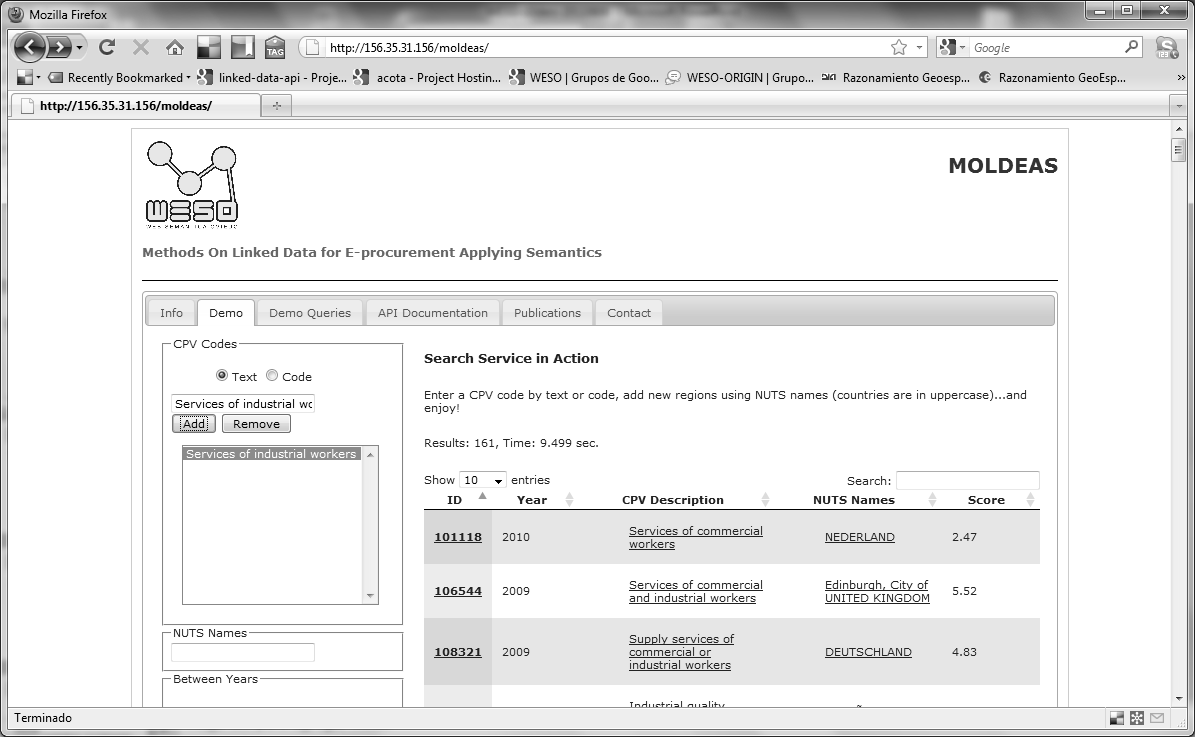
\includegraphics[width=14cm]{images/phd/moldeas/moldeas-web}
\caption{Ejemplo de pantalla inicial en \texttt{moldeas-web}.}
\label{fig:moldeas-web-screen}
\end{figure}


\item Una vez que el usuario ha seleccionado su perfil de búsqueda se ejecuta 
el proceso de recuperación de información presentando los resultados en forma 
tabular y mediante el uso de Exhibit, ver Figura~\ref{fig:moldeas-results-screen}. El usuario 
puede modificar su perfil de búsqueda y las consultas se lanzarán automáticamente una 
vez se detecten cambios. De la misma forma, el usuario puede filtrar los resultados, 
ordenarlos por relevancia, por sector, etc. e incluso visualizar la región en la 
que se han publicado los anuncios de licitación. La idea subyacente a esta 
interacción reside en que el usuario disponga del completo control de la presentación 
de los resultados obtenidos.


\begin{figure}[!htb]
\centering
	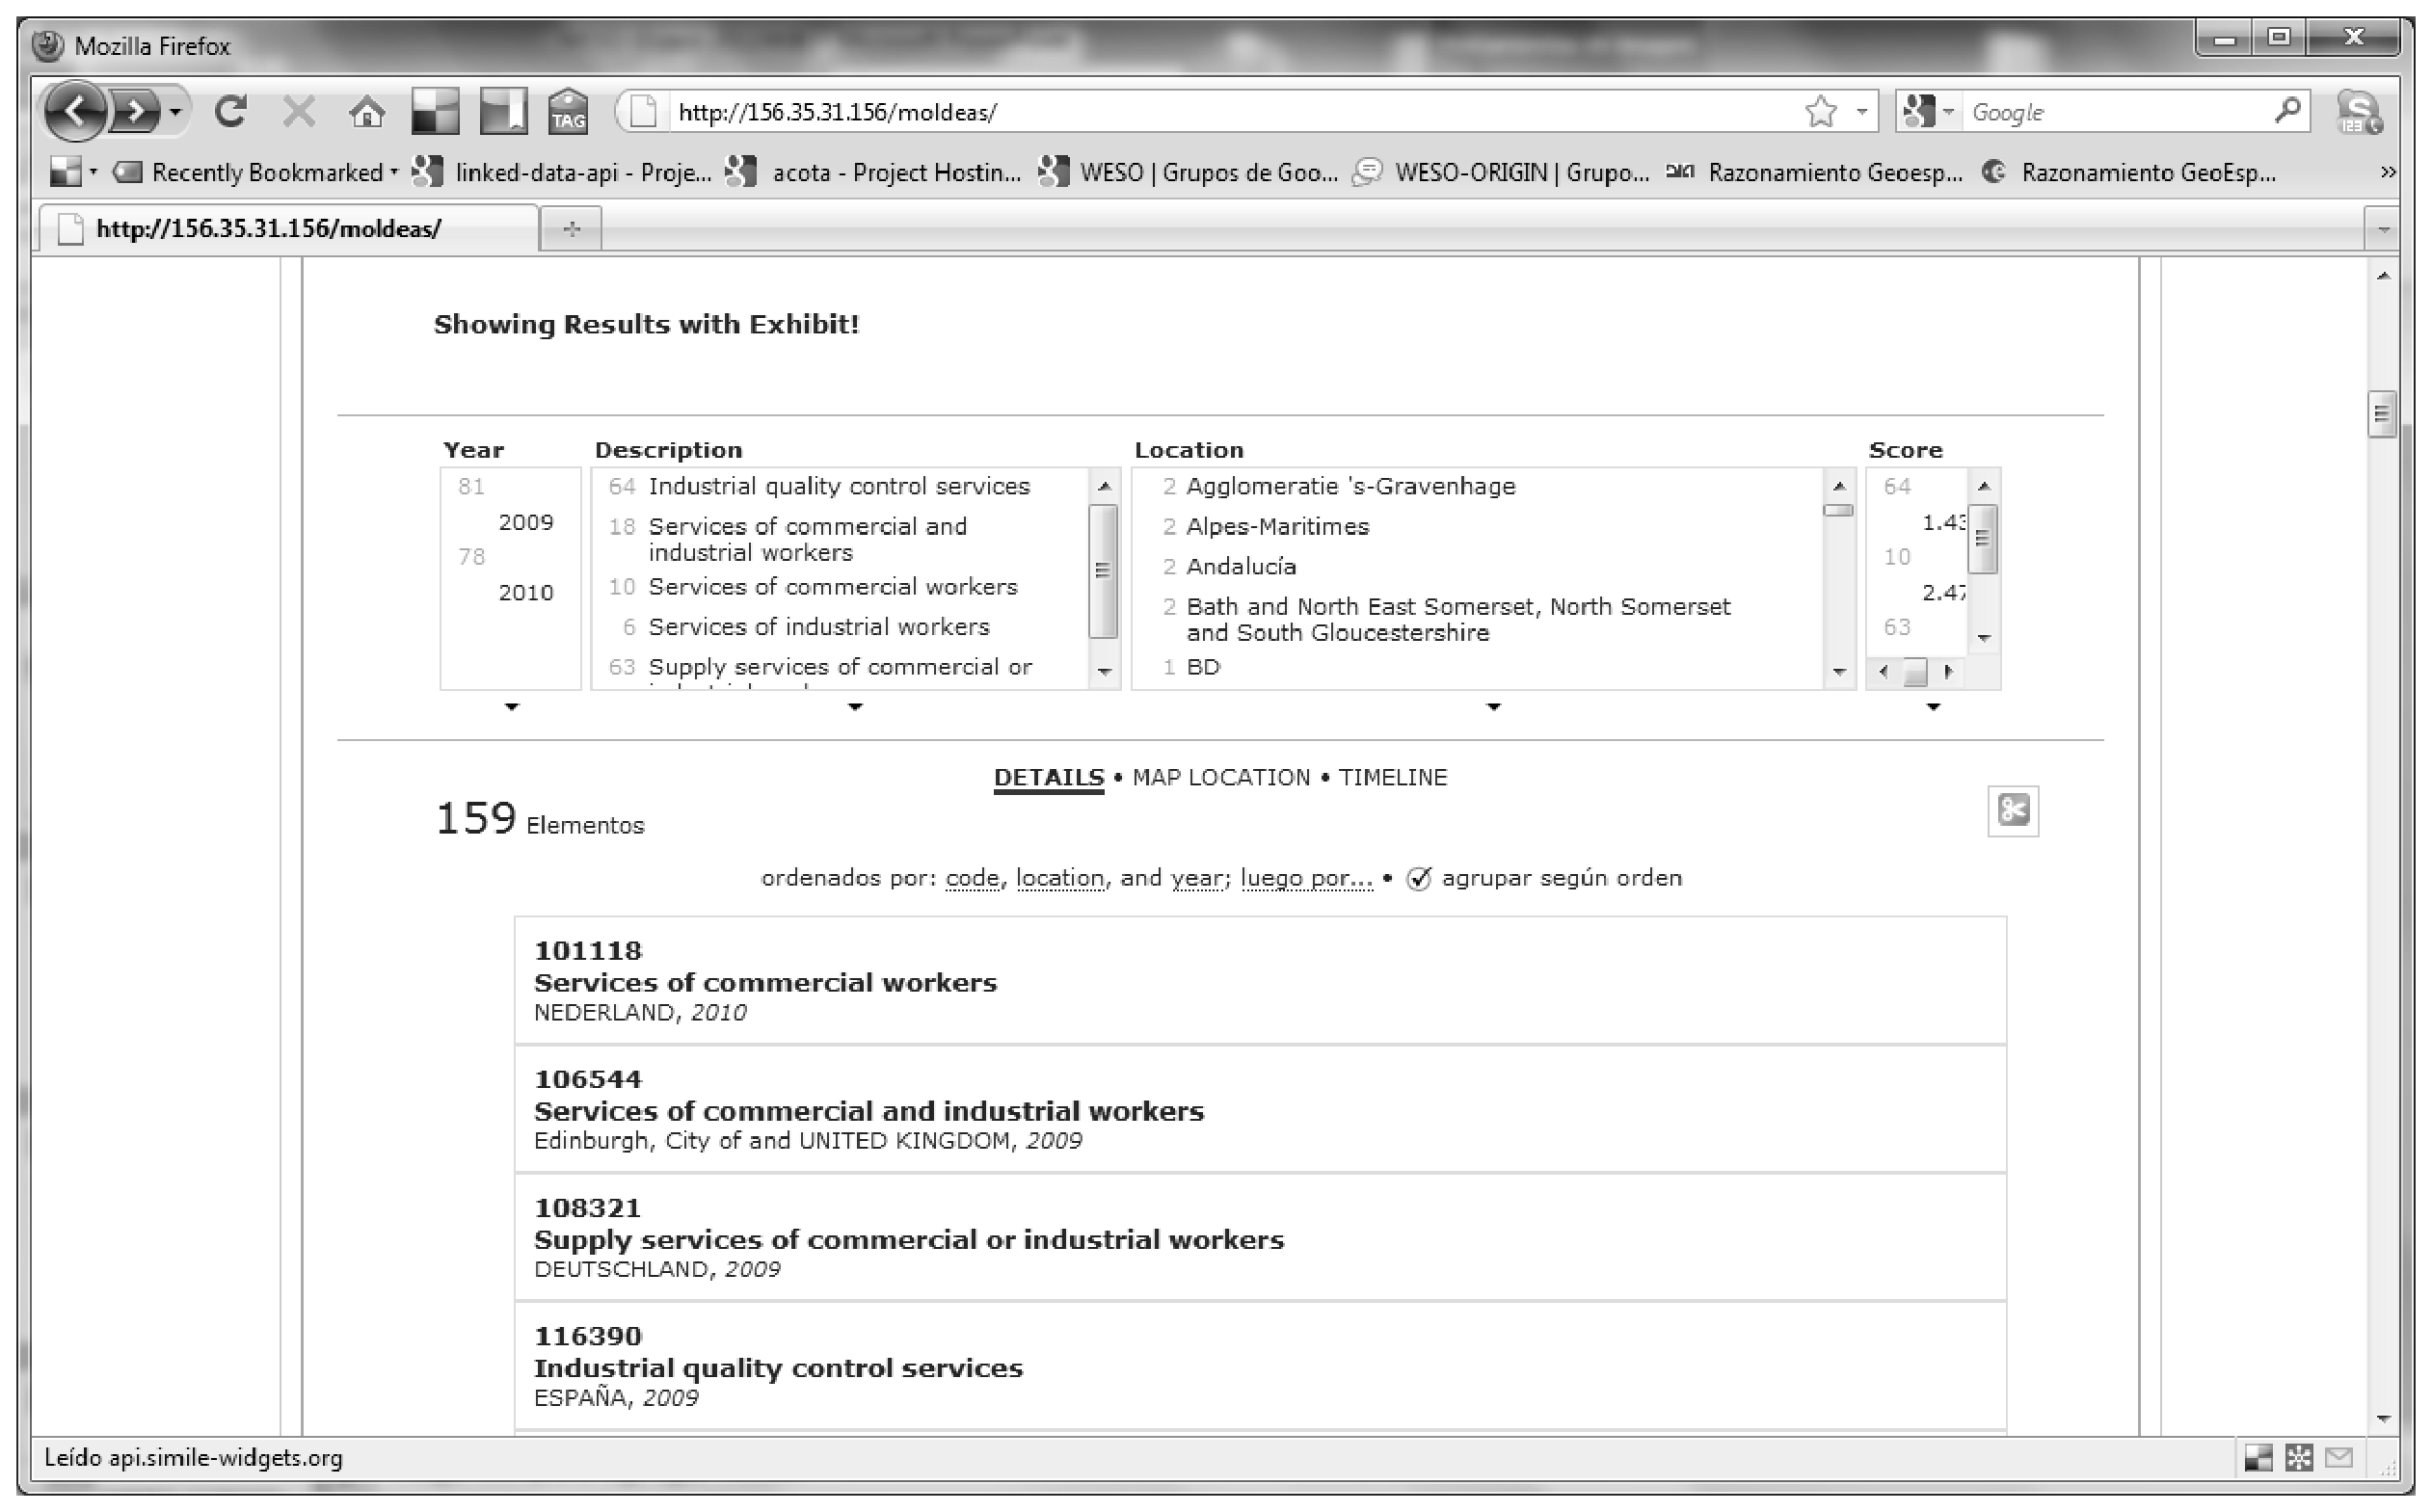
\includegraphics[width=14cm]{images/phd/moldeas/moldeas-results}
\caption{Ejemplo de pantalla de resultados en \texttt{moldeas-web}.}
\label{fig:moldeas-results-screen}
\end{figure}


\item En los resultados de búsqueda todas las \gls{URI}s presentadas son referenciables siguiendo 
las buenas prácticas de \linkeddata que han guiado la promoción de los datos a esta iniciativa. 
Es por ello que los datos propios del \dataset \gls{RDF} se pueden consultar y navegar a través de sus 
relaciones mediante el uso de un \linkeddata \textit{front-end}, en este caso Pubby, ver Figura~\ref{fig:moldeas-pubby-screen}. 


\begin{figure}[!htb]
\centering
	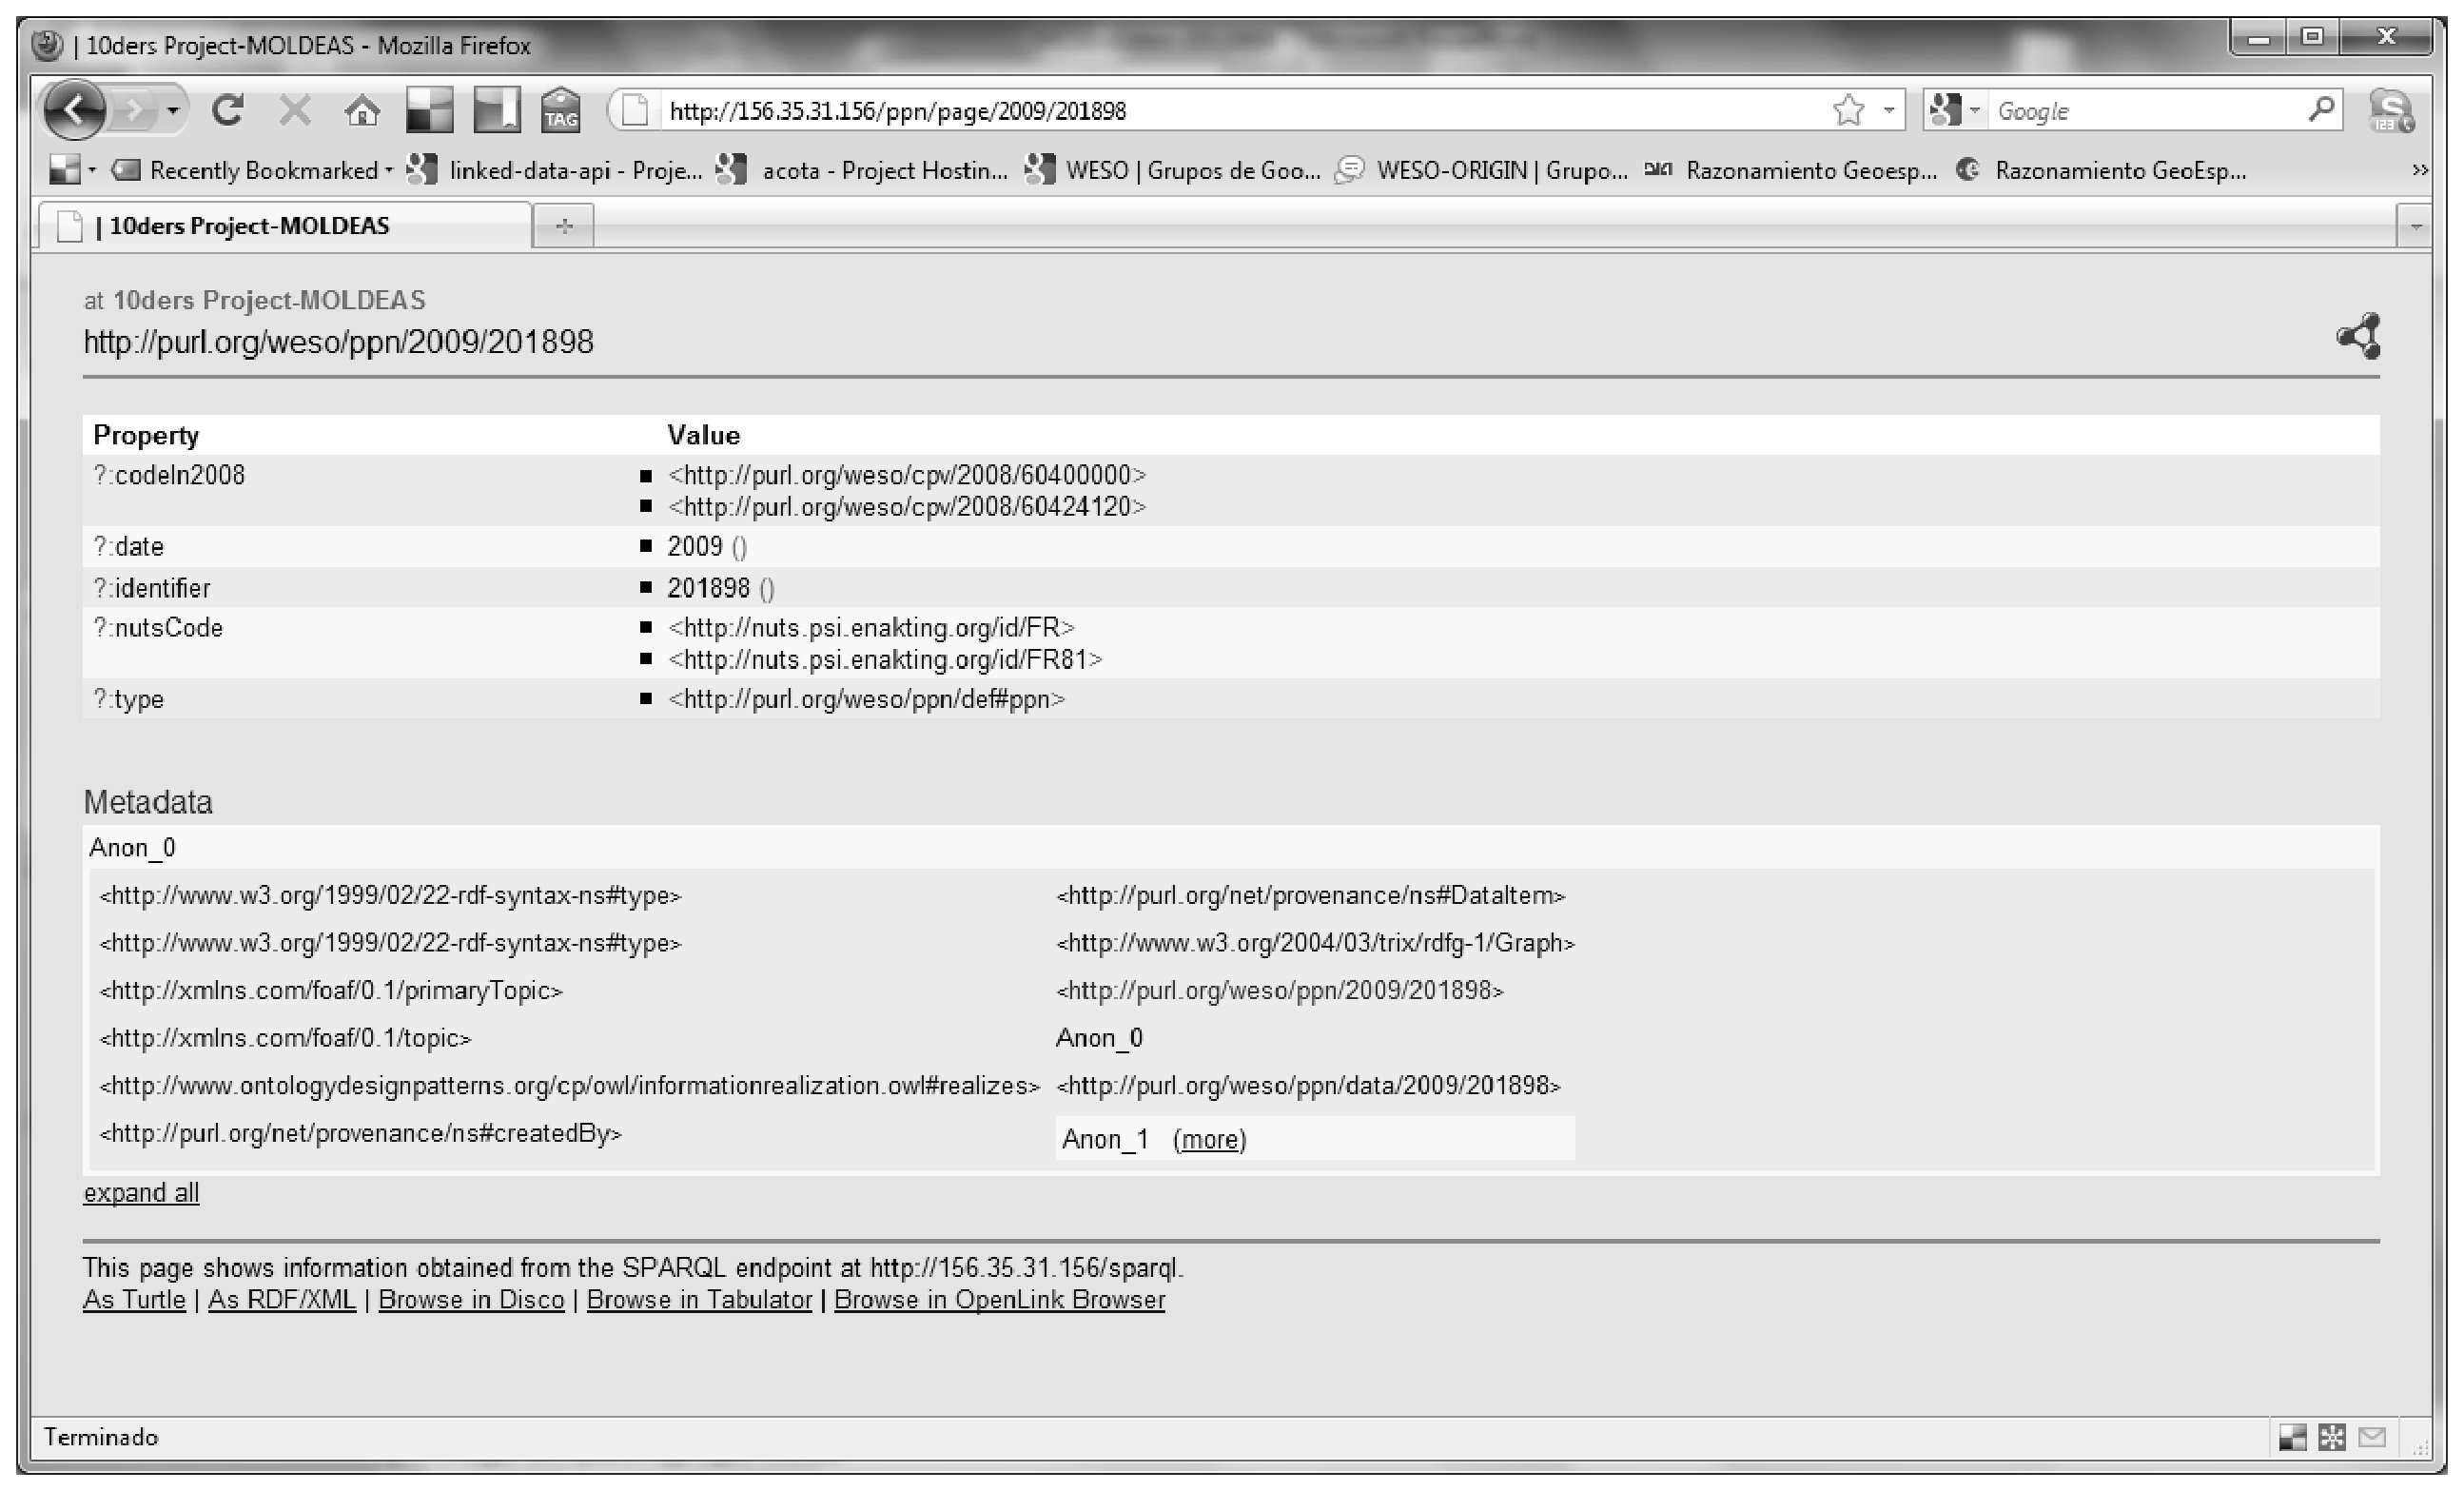
\includegraphics[width=14cm]{images/phd/moldeas/moldeas-pubby}
\caption{Acceso a los datos enlazados mediante Pubby.}
\label{fig:moldeas-pubby-screen}
\end{figure}


\item Finalmente y con el objetivo de ejemplificar el uso de \gls{SPARQL} y las posibilidades 
de consultas al \texttt{endpoint} se han creado una serie de consultas representativas 
para que los usuarios más técnicos tengan la posibilidad de configurar y crear sus propias 
consultas, ejecutándolas y obteniendo los resultados directamente. Para suministrar esta funcionalidad 
se ha utilizado la herramienta \gls{SNORQL}, ver Figura~\ref{fig:moldeas-snorql-screen}.

\begin{figure}[!htb]
\centering
	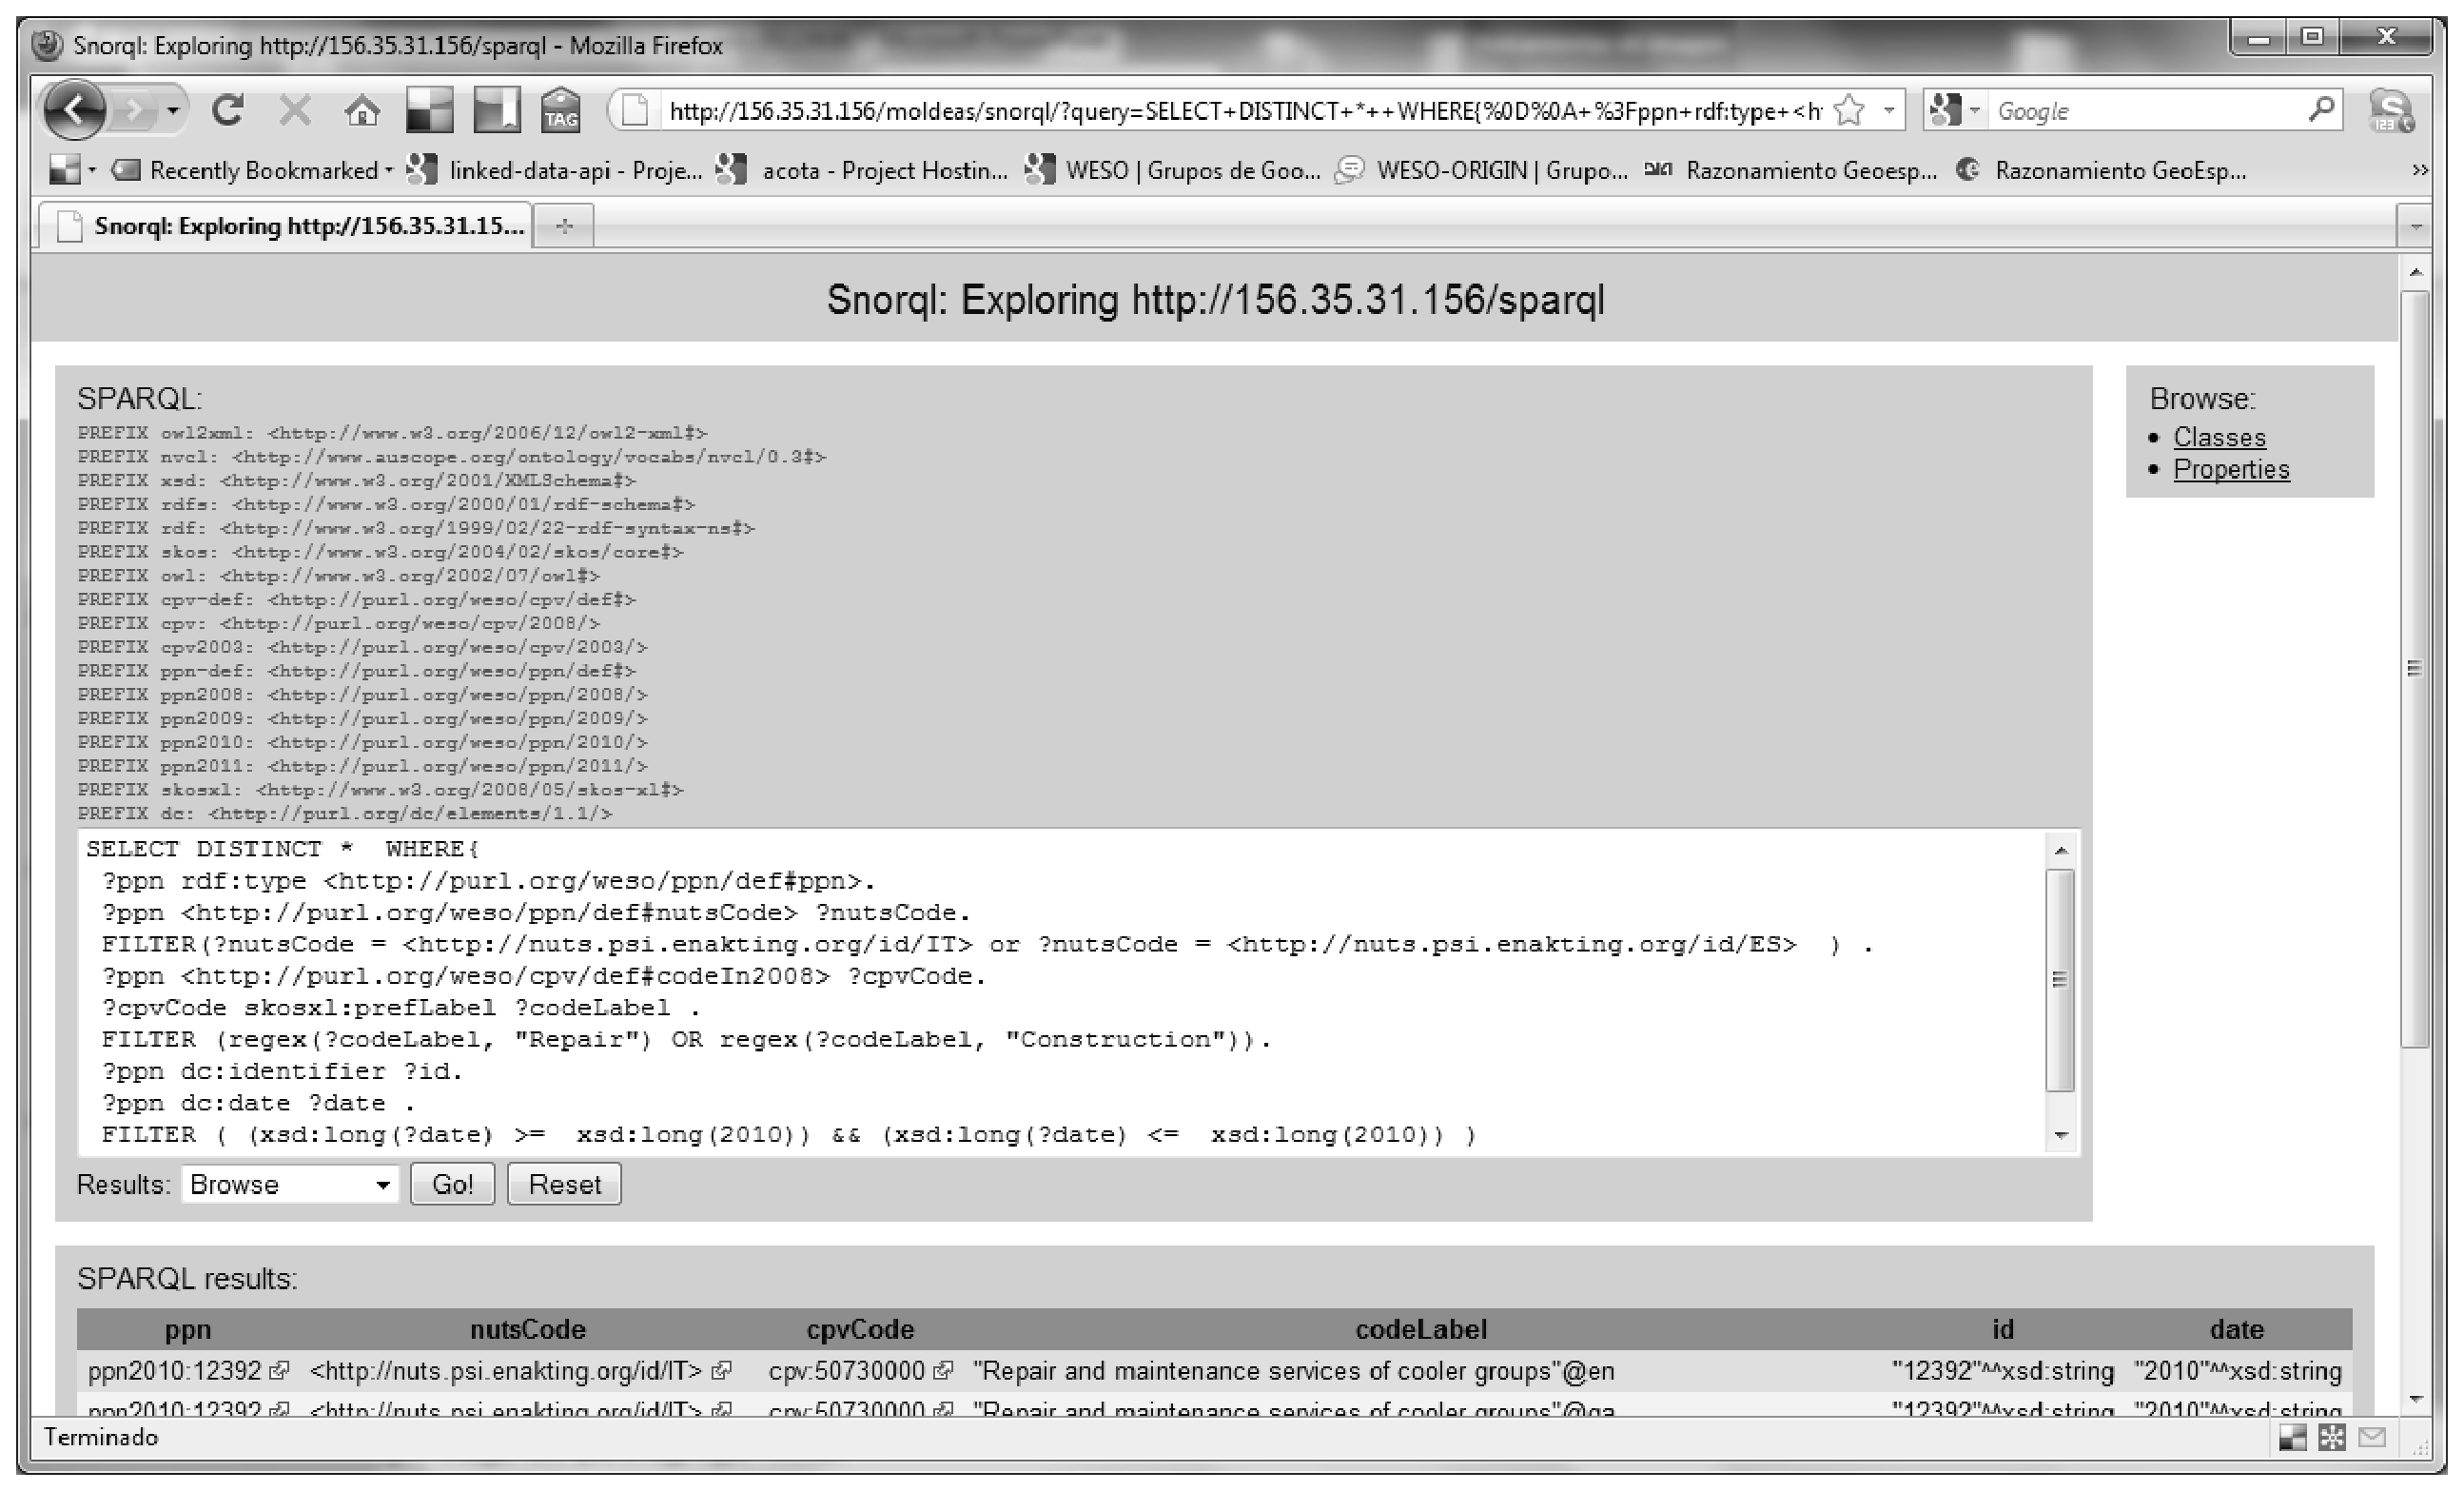
\includegraphics[width=14cm]{images/phd/moldeas/moldeas-snorql}
\caption{Consulta a los datos enlazados mediante SNORQL.}
\label{fig:moldeas-snorql-screen}
\end{figure}



\end{enumerate}









\appendix
\chapter{\label{capitulo:tablas}Tablas de Validación}\label{tablas-validacion-apen}
\section{Consideraciones sobre las Tablas de Validación}
El objetivo de esta sección es presentar las tablas de validación que se utilizan para realizar 
la evaluación del grado de cumplimiento de criterios relativos a las iniciativas de 
\linkeddata y \opendata, para verificar que verdaderamente los datos generados se pueden enclavar 
bajo estos enfoques, asegurando por tanto los beneficios y ventajas propugnados por los mismos. Para la elaboración 
y diseño de estas tablas se ha considerado el trabajo relacionado presentado en la Sección~\ref{metodologias}, así 
como la experiencia personal en la investigación y desarrollo de distintas actividades relacionadas con estas iniciativas. 

Los criterios presentados en estas tablas pueden adquirir tres valores:
\begin{itemize}
 \item Valor positivo, \si, si es un criterio que debe tener y se cumple.
 \item Valor negativo, \no, si es un criterio que debe tener y no se cumple.
 \item Valor no aplicable, \na, si es un criterio que se desconoce, se solapa con otro o bien 
o no está asociado al enfoque evaluado.
\end{itemize}

Para ejemplificar una validación en las tablas siguientes se realiza la valoración de un conjunto 
de datos de referencia en general, y \datasets RDF en particular. El grado de cumplimiento de criterios 
ideal se fija en un total de $173$ criterios positivos (\si) y $23$ no aplicables (\na) realizando 
una encuesta total de $196$ criterios de valoración. De esta forma, es posible delimitar si una enfoque 
pertenece a la iniciativa de \opendata, \linkeddata, a la nube de datos enlazados abiertos o 
a un registro \gls{CKAN}, adicionalmente se valora el grado en el que los procesos de producción, publicación, 
consumo, validación y realimentación de los conjuntos de datos se facilitan. 

\subsection{Tabla de Validación $T^{1}$}
En la Tabla~\ref{table:validation-t1} se recogen criterios de validación relativos a los 
procesos de producción, publicación y consumo de datos enlazados, realizando un especial hincapié 
en el diseño de \gls{URI}s, modelado de información y datos utilizando tecnologías semánticas así como factores relativos a la 
descripción de la metainformación de los recursos. Se ha realizado la valoración ideal 
de un \dataset \gls{RDF} de referencia que contaría con $60$ criterios positivos (\si) y $9$ no aplicables 
(\na).

\begin{longtable}[c]{|l|p{7cm}|c|} 
\hline 
  \textbf{ID} & \textbf{Pregunta} &  \textbf{Cumplimiento} \\\hline
\endhead  
  1& \multicolumn{2}{|c|}{\textbf{\textit{Uso de URIs}}} \\ \hline
  1.1&  ¿Las URIs utilizadas permiten acceder a los recursos, \textit{Minting HTTP URIs}? & \si \\ \hline 
  1.2&  ¿El \textit{namespace} utilizado en las URIs está bajo nuestro control? & \si \\ \hline
  1.3&  ¿Se utiliza el esquema  HTTP? &\si  \\ \hline
  1.4&  ¿Las URIs siguen las directrices de \textit{Cool URIs}? &\si  \\ \hline
  1.5&  ¿Se utilizan \textit{hash URIs}? & \na  \\ \hline
  1.6&  ¿Se utilizan \textit{slash URIs}? & \si  \\ \hline
  1.7&  ¿Se utilizan \textit{param URIs}? & \na  \\ \hline
  1.8&  ¿No se incluyen detalles de implementación en la URI? & \si  \\ \hline
  1.9&  ¿Se utilizan claves primarias para identificar los recursos, ID URIs? & \si  \\ \hline
  1.10&  ¿Se utilizan nombres para identificar a los recursos, \textit{Meaningful URIs}? & \na  \\ \hline
  1.11&  ¿Se ha definido una URI base para los recursos? & \si  \\ \hline
  1.12&  ¿Se ha definido una URI base para el modelo formal? & \si  \\ \hline
  1.13&  ¿Se ha definido un esquema de URIs para el \dataset RDF? & \si  \\ \hline
  1.14&  ¿Se ha definido un esquema de URIs para el modelo formal? & \si  \\ \hline
  1.15&  ¿Se incluye metainformación en las URIs? & \si  \\ \hline
 2&\multicolumn{2}{|c|}{\textbf{\textit{Descripción de recursos en \gls{RDF}}}}\\ \hline
  2.1& ¿Se utilizan vocabularios como \gls{SKOS}, RDFS, OWL para modelar el dominio?& \si  \\ \hline
  2.2& ¿Se reutilizan vocabularios de acuerdo a su uso y actualización?& \si  \\ \hline
  2.3& ¿Se utilizan anotaciones de RDFS o SKOS?& \si  \\ \hline
  2.4& ¿Se relacionan las clases y propiedades con otras ya existentes?& \si \\ \hline
  2.5& ¿Se reutilizan las clases y propiedades ya existentes?& \si  \\ \hline
  2.6& ¿Se definen nuevas clases y propiedades?&\si  \\ \hline
  2.7& ¿Se enriquecen las descripciones RDF con otros \datasets RDF?& \si  \\ \hline
  2.8& ¿Se describe parcialmente los recursos de otros \datasets RDF a los que se enlaza desde el actual?& \no  \\ \hline
  2.9& ¿Se añade metainformación a cada recurso RDF individualmente?& \si  \\ \hline
  2.10& ¿Son las descripciones de los recursos RDF navegables?& \si  \\ \hline
  2.11& ¿Se provee información útil del recurso RDF a través de la URI?& \si  \\ \hline
  2.12& ¿Son las URIs reutilizadas referenciables?& \si  \\ \hline  
 3&\multicolumn{2}{|c|}{\textbf{\textit{Descripción del \dataset RDF}}}\\ \hline
  3.1& ¿Se ha definido una \gls{URI} para el \dataset RDF? & \si  \\ \hline
  3.2& ¿Se utiliza el vocabulario \gls{voID} para describir el \dataset RDF? & \si  \\ \hline
  3.3& ¿Se utiliza el \textit{Semantic Sitemaps} para describir el \dataset RDF? & \na  \\ \hline
  3.4& ¿Se provee información de \textit{provenance}? & \si  \\ \hline
  3.5& ¿Se provee licencia de uso, información sobre derechos de copia, etc.?&  \si  \\ \hline
  3.6& ¿Se provee información sobre la autoría? & \si  \\ \hline
  3.7& ¿Se proveen ejemplos de uso del \dataset RDF? & \si  \\ \hline
  3.8& ¿Se utilizan anotaciones de RDFS o SKOS?&  \si  \\ \hline
  3.9& ¿Se utilizan anotaciones multilingües RDFS o SKOS?& \si  \\ \hline
 4&\multicolumn{2}{|c|}{\textbf{\textit{Otros}}}\\ \hline
  4.1& ¿Se utilizan herramientas automáticas para la producción de RDF?& \si  \\ \hline
  4.2& ¿Se consolidan parte de los datos en RDF?& \no  \\ \hline
  4.3& ¿Se realiza la reconciliación de entidades de forma automática?& \no  \\ \hline
  4.4& ¿Los datos son dinámicos?& \na  \\ \hline
  4.5& ¿Los datos son estáticos?& \si  \\ \hline
  4.6& ¿El tamaño del \dataset es del orden de millones de tripletas?& \si  \\ \hline
  4.7& ¿El tamaño del \dataset es del orden de billones de tripletas?& \na  \\ \hline
5&\multicolumn{2}{|c|}{\textbf{\textit{Publicación de \linkeddata}}}\\ \hline
  5.1&  ¿Se publica un volcado de los datos en RDF? & \no  \\ \hline 
  5.2&  ¿Se utiliza algún método de publicación de datos enlazados? & \si  \\ \hline
  5.3&  ¿Se provee algún lenguaje de consulta formal? & \si  \\ \hline
  5.4&  ¿Se provee un \textit{endpoint de \gls{SPARQL}}? & \si  \\ \hline
  5.5&  ¿Se provee negociación de contenido? & \si  \\ \hline
  5.6&  ¿Se pueden referenciar los recursos desde otros documentos tipo \gls{HTML}? & \si  \\ \hline    
  5.7&  ¿Se provee un \linkeddata \textit{Frontend}? & \si  \\ \hline  
  5.8&  ¿Se provee metainformación del \dataset RDF? & \si  \\ \hline
  5.9&  ¿Se difunde el \dataset RDF en distintos medios tipo CKAN, Prefix.cc, etc.? & \si  \\ \hline
  5.10&  ¿Se publica algún API o servicio web para la consulta de los datos? & \si  \\ \hline
  5.11&  ¿Existe alguna restricción en la consulta de los datos? & \no  \\ \hline
  5.12&  ¿Se establece algún mecanismo de privacidad? & \no  \\ \hline
  5.13&  ¿Se informa del tamaño del \dataset? & \si  \\ \hline  
  5.14&  ¿Se publican los datos RDF como un fichero estático? & \na  \\ \hline
  5.15&  ¿Se publican los datos RDF bajo demanda desde base de datos?& \na  \\ \hline
  5.16&  ¿Se publican los datos RDF en un repositorio? & \si  \\ \hline    
  5.17&  ¿Se publican los datos RDF bajo demanda desde una aplicación? & \si  \\ \hline
  5.18&  ¿Se publican los datos con información temporal y evolución en el tiempo?& \no  \\ \hline     
  5.19&  ¿Se proveen ejemplos para depuración y consumo? & \si  \\ \hline        
  5.20&  ¿Se proveen alias a ciertos directorios o nombres? & \si  \\ \hline
  5.21&  En caso de error, ¿se devuelve algún recurso por omisión? &  \no  \\ \hline      
  5.22&  ¿Se utilizan protocolos estándar? & \si  \\ \hline    
  5.23&  ¿Se provee algún mecanismo de realimentación? & \no  \\ \hline    
  5.24&  ¿Se provee documentación sobre los datos publicados? & \si  \\ \hline
  5.25&  ¿Se proveen estadísticas de los datos publicados? & \si  \\ \hline    
  5.26&  ¿Se utilizan mecanismos de sellado en el tiempo o similares? & \si  \\ \hline            
 \hline
\caption{$T^{1}$-Tabla de Validación de Características \linkeddata.}\label{table:validation-t1}\\    
\end{longtable}



\subsection{Tabla de Validación $T^{2}$}

En la Tabla~\ref{table:validation-t2} se recogen criterios de validación relativos a los 
a los patrones de diseño utilizados para la generación de datos enlazados. Si bien su uso no es obligatorio, 
la idea subyacente coincide con los patrones de diseño en ingeniería del software en los cuales 
se ofrecen soluciones para casuísticas habituales con el objetivo de mejorar tanto los procesos de 
producción, publicación, consumo, validación y realimentación. Se ha realizado la valoración ideal 
de un \dataset \gls{RDF} de referencia que contaría con $44$ criterios positivos (\si), incluyendo la aplicación 
de todos los patrones, se ha tomado esta decisión para obtener una medida del grado de aplicación de los 
mismos ya que en muchos casos la información generada en un \dataset RDF puede utilizar unos u otros no es 
conveniente plantear su uso como disyuntivo.


\begin{longtable}[c]{|l|p{7cm}|c|} 
\hline 
  \textbf{ID} & \textbf{Pregunta} &  \textbf{Cumplimiento}  \\\hline
\endhead 
   1& \multicolumn{2}{|c|}{\textbf{\textit{Identifier Patterns}}}\\ \hline
  1.1 &  \textit{Hierarchical \gls{URI}s} &\si \\ \hline
  1.2 &  \textit{Literal Keys} &\si \\ \hline
  1.3 &  \textit{Natural Keys} &\si \\ \hline
  1.4 &  \textit{Patterned URIs} &\si \\ \hline
  1.5 &  \textit{Proxy URIs} &\na \\ \hline
  1.6 &  \textit{Shared Keys} &\na \\ \hline
  1.7 &  \textit{\gls{URL} Slug} &\na \\ \hline    
    2& \multicolumn{2}{|c|}{\textbf{\textit{Modelling Patterns}}}\\ \hline
  2.1 &  \textit{Custom Datatype} &\si \\ \hline    
  2.2 &  \textit{Index Resources} &\na \\ \hline    
  2.3 &  \textit{Label Everything} &\si \\ \hline     
  2.4 &  \textit{Link Not Label} &\si \\ \hline    
  2.5 &  \textit{Multi-Lingual Literal} &\si \\ \hline    
  2.6 &  \textit{N-Ary Relation} &\na \\ \hline    
  2.7 &  \textit{Ordered List} &\na \\ \hline     
  2.8 &  \textit{Ordering Relation} &\na \\ \hline     
  2.9 &  \textit{Preferred Label} &\si \\ \hline    
  2.10 &  \textit{Qualified Relation} &\si \\ \hline   
  2.11 &  \textit{Reified Statement} &\na \\ \hline    
  2.12 &  \textit{Topic Relation} &\si \\ \hline      
  2.13 &  \textit{Typed Literal} &\si \\ \hline        
    3& \multicolumn{2}{|c|}{\textbf{\textit{Publishing Patterns}}}\\ \hline
  3.1 &  \textit{Annotation} &\si \\ \hline    
  3.2 &  \textit{Autodiscovery} &\si \\ \hline    
  3.3 &  \textit{Document Type} &\si \\ \hline     
  3.4 &  \textit{Edit Trail} &\no \\ \hline    
  3.5 &  \textit{Embedded Metadata} &\si \\ \hline    
  3.6 &  \textit{Equivalence Links} &\si \\ \hline    
  3.7 &  \textit{Link Base} &\si \\ \hline     
  3.8 &  \textit{Materialize Inferences} &\na \\ \hline     
  3.9 &  \textit{Named Graphs} &\si \\ \hline    
  3.10 &  \textit{Primary Topic Autodiscovery} &\si \\ \hline    
  3.11 &  \textit{Progressive Enrichment} &\si \\ \hline      
  3.12 &  \textit{See Also} &\si \\ \hline    
        4& \multicolumn{2}{|c|}{\textbf{\textit{Application Patterns}}}\\ \hline
  4.1 &  \textit{Assertion Query} &\si \\ \hline    
  4.2 &  \textit{Blackboard} &\si \\ \hline    
  4.3 &  \textit{Bounded Description} &\si \\ \hline     
  4.4 &  \textit{Composite Descriptions} &\si \\ \hline    
  4.5 &  \textit{Follow Your Nose}&\no \\ \hline    
  4.6 &  \textit{Missing Isn't Broken} &\no \\ \hline    
  4.7 &  \textit{Parallel Loading} &\no \\ \hline     
  4.8 &  \textit{Parallel Retrieval} &\no \\ \hline
  4.9 &  \textit{Resource Caching} &\no \\ \hline    
  4.10 &  \textit{Schema Annotation} &\si \\ \hline    
  4.11 &  \textit{Smushing} &\si \\ \hline
  4.12 &  \textit{Transformation Query} &\no \\ \hline        
 
\hline
\caption{$T^{2}$-Tabla de Validación de \textit{Linked Data Patterns}.}\label{table:validation-t2}\\    
\end{longtable}



\subsection{Tabla de Validación $T^{3}$}
En la Tabla~\ref{table:validation-t3} se recogen los principios de \linkeddata que sirven 
para valorar si un enfoque se encuentra dentro de esta iniciativa. Se ha realizado la valoración ideal 
de un \dataset \gls{RDF} de referencia que contaría con $4$ criterios positivos (\si).

\begin{longtable}[c]{|l|p{7cm}|c|} 
\hline 
  \textbf{ID} & \textbf{Pregunta} &  \textbf{Cumplimiento}  \\\hline
\endhead
   1.1&\textit{Use \gls{URI}s as names for things} & \si  \\ \hline
   1.2&\textit{When someone looks up a URI, provide useful information, using the standards (RDF*, \gls{SPARQL})} & \si \\ \hline  
   1.3&\textit{Include links to other URIs} & \si \\ \hline    
   1.4&\textit{Use \gls{HTTP URI}s} & \si \\ \hline    
   \hline
  \caption{$T^{3}$-Tabla de Validación de Principios de \linkeddata.}
  \label{table:validation-t3}
\end{longtable}

\subsection{Tabla de Validación $T^{3}_1$}
En la Tabla~\ref{table:validation-t31} y en combinación con la anterior, se recogen los criterios 
relacionados con el modelo de $\star$ propuesto por Tim Berners-Lee y de esta forma se puede 
establecer el nivel de datos enlazados de un determinado \dataset \gls{RDF}, el valor de referencia 
máximo contaría con $5$ criterios positivos (\si), uno por cada $\star$.

\begin{longtable}[c]{|l|p{7cm}|c|} 
\hline 
  \textbf{ID} & \textbf{Pregunta} &  \textbf{Cumplimiento}  \\\hline
\endhead
 
   1.1&$\star$	& \si \\ \hline 

1.2&$\star \star$	 & \si \\ \hline 

1.3&$\star \star \star$	& \si  \\ \hline 

1.4&$\star \star \star \star$ & \si \\ \hline 
 
1.5&$\star \star \star \star \star$ & \si \\ \hline 
  \hline
  \caption{$T^{3}_1$-Tabla de Validación del Modelo $\star$.}
  \label{table:validation-t31}
\end{longtable}



\subsection{Tabla de Validación $T^{4}$}
En la Tabla~\ref{table:validation-t4} se recogen los principios de \opendata que sirven 
para valorar si un enfoque se encuentra dentro de esta iniciativa. Se ha realizado la valoración ideal 
de un \dataset \gls{RDF} de referencia, o en general un conjunto de datos públicos, contaría con $8$ criterios positivos (\si).
\newpage
\begin{longtable}[c]{|l|p{7cm}|c|} 
\hline 
  \textbf{ID} & \textbf{Pregunta} &  \textbf{Cumplimiento}  \\\hline
\endhead
  \multicolumn{3}{|c|}{\textbf{8 Principios}}  \\ \hline
   1.1& \textit{Complete} & \si  \\ \hline
   1.2&\textit{Primary} & \si  \\ \hline  
   1.3&\textit{Timely} & \si  \\ \hline  
   1.4&\textit{Accessible} & \si  \\ \hline  
   1.5&\textit{Machine processable} & \si  \\ \hline  
   1.6&\textit{Non-Discriminatory} & \si  \\ \hline  
   1.7&\textit{Non-Proprietary} &\si  \\ \hline
   1.8&\textit{License-free} & \si  \\ \hline                                                               
  \hline
  \caption{$T^{4}$-Tabla de Validación de Principios de \opendata.}
  \label{table:validation-t4}
\end{longtable}

\subsection{Tabla de Validación $T^{4}_1$}
En la Tabla~\ref{table:validation-t41} se recogen beneficios y ventajas de la aplicación de los principios de \opendata. 
Se ha realizado la valoración ideal de un \dataset \gls{RDF}, o en general de un conjunto de datos públicos, 
de referencia contaría con $14$ criterios positivos (\si).

\begin{longtable}[c]{|l|p{7cm}|c|} 
\hline 
  \textbf{ID} & \textbf{Pregunta} &  \textbf{Cumplimiento}  \\\hline
\endhead
   \multicolumn{2}{|c|}{\textbf{Producción}}  \\ \hline
   1.1& ¿Se ha definido una misión y estrategia para la apertura de los datos? & \no  \\ \hline
   1.2& ¿Los datos proceden de una fuente segura? & \no  \\ \hline
   1.3& ¿Se puede conocer la procedencia de los datos? & \si  \\ \hline    
   1.4& ¿Existe algún mecanismo para asegurar la calidad de los datos? & \si  \\ \hline  
  \multicolumn{2}{|c|}{\textbf{Ventajas}}  \\ \hline
   2.1& ¿Facilitan los datos la inclusión? & \si  \\ \hline
   2.2& ¿Mejoran la transparencia? & \si  \\ \hline    
   2.3& ¿Existe alguna responsabilidad sobre los datos? & \no  \\ \hline
  \multicolumn{2}{|c|}{\textbf{Beneficios}}  \\ \hline
   3.1& ¿Pueden las aplicaciones servirse de estos datos para generar servicios, reutilización? & \si  \\ \hline
   3.2& ¿Se pueden generar múltiples vistas de los datos? & \si  \\ \hline
   3.3& ¿Se pueden integrar con otras fuentes de datos? & \si  \\ \hline     
   \multicolumn{2}{|c|}{\textbf{Consumo}}  \\ \hline
   4.1& Uso de anotaciones & \si  \\ \hline        
   4.2& ¿Se provee un \gls{API} o servicio web de consumo? & \si  \\ \hline
   4.3& ¿Se provee algún mecanismo de sindicación para obtener los datos?& \no  \\ \hline
   4.4& ¿Existe algún modelo formal o especificación de los datos publicados? & \si  \\ \hline                                                             
  \hline
  \caption{$T^{4}_1$-Tabla de Validación sobre Características de \opendata.}
  \label{table:validation-t41}
\end{longtable}



\subsection{Tabla de Validación $T^{5}$}
En la Tabla~\ref{table:validation-t5} se recogen los criterios para pertenecer a la nube de datos 
enlazados y abiertos. Estos criterios son complementarios a los señalados en las tablas anteriores 
en el sentido del grado de cumplimiento de \linkeddata y \opendata. Sin embargo, la importancia 
de esta valoración reside en calibrar el grado de reutilización de información y la capacidad 
de difusión del \dataset \gls{RDF}. Es por ello que se fija una valoración de referencia de $5$ criterios 
positivos (\si).

\begin{longtable}[c]{|l|p{7cm}|c|} 
\hline 
  \textbf{ID} & \textbf{Pregunta} &  \textbf{Cumplimiento}  \\\hline
\endhead
   1& ¿Son los recursos \gls{RDF} accesibles mediante \gls{HTTP} o \gls{HTTPS}? & \si  \\ \hline
   2& ¿Se provee negociación de contenido? & \si  \\ \hline
   3& ¿El \dataset contiene más de 1000 tripletas? & \si  \\ \hline
   4& ¿Se provee, al menos, 50 enlaces a \datasets ya disponibles en el diagrama? & \si \\ \hline
   5& ¿Se provee acceso al \dataset completo? & \si  \\ \hline
  \hline
  \caption{$T^{5}$-Tabla de Validación sobre Características para pertenecer a \textit{The Linking Open Data Cloud}.}
  \label{table:validation-t5}
\end{longtable}



\subsection{Tabla de Validación $T^{6}$}
En la Tabla~\ref{table:validation-t6} se recogen los criterios para pertenecer a un registro \gls{CKAN}, complementario 
y obligatorio a la pertenencia a la nube de datos enlazados y abiertos. Este valoración cobra especial relevancia 
si el \dataset \gls{RDF} va a ser publicado para su reutilización por terceros, en el caso de datos enlazados a nivel 
privado no tendría tanta trascendencia. La valoración de un \dataset RDF de referencia se fija 
en $33$ criterios positivos (\si) y $14$ criterios positivos (\na).

\begin{longtable}[c]{|l|p{7cm}|c|} 
\hline 
  \textbf{ID} & \textbf{Pregunta} &  \textbf{Cumplimiento}  \\\hline
\endhead
  1&\multicolumn{2}{|c|}{\textbf{Standard CKAN fields}}  \\ \hline
  1.1&  \textit{Name} & \si  \\ \hline
  1.2 &  \textit{Title} & \si  \\ \hline
  1.3 &  \textit{URL} & \si  \\ \hline
  \multicolumn{3}{|c|}{\textbf{Enhanced CKAN fields}}  \\ \hline
   1.4&  \textit{Version} & \si  \\ \hline
   1.5&  \textit{Notes} & \no  \\ \hline
   1.6&  \textit{Author} & \si  \\ \hline
   1.7&  \textit{Author email} &\si  \\ \hline
   1.8&  \textit{License} &\si  \\ \hline
   \multicolumn{3}{|c|}{\textbf{Custom CKAN fields}}  \\ \hline
   1.9&  \textit{shortname} & \si  \\ \hline
   1.10&  \textit{license\_link} & \si  \\ \hline
   1.11&  \textit{sparql\_graph\_name} & \no  \\ \hline
   1.12&  \textit{namespace} & \si  \\ \hline
   1.13&  \textit{triples} & \si  \\ \hline
   1.14&  \textit{links:xxx} &\si  \\ \hline
  2&\multicolumn{2}{|c|}{\textbf{CKAN tags}}  \\ \hline
  2.1&  \textit{<topic>} &\si \\ \hline
  \multicolumn{3}{|c|}{\textbf{Metainformation CKAN tags}}  \\ \hline  
  2.2&\textit{format-<prefix>}&\si \\ \hline
  2.3&\textit{no-proprietary-vocab}&\na \\ \hline
  2.4 &\textit{deref-vocab}&\si \\ \hline
  2.5&\textit{no-deref-vocab}&\na \\ \hline
  2.6&\textit{vocab-mappings}&\si \\ \hline
  2.7&\textit{no-vocab-mappings}&\na \\ \hline
  2.8&\textit{provenance-metadata}&\si \\ \hline
  2.9&\textit{no-provenance-metadata}&\na \\ \hline
  2.10&\textit{license-metadata}&\si \\ \hline
  2.11&\textit{no-license-metadata}&\na \\ \hline	
  2.12&\textit{published-by-producer}&\na \\ \hline
  2.13&\textit{published-by-third-party}&\si \\ \hline		
  2.14&\textit{limited-sparql-endpoint}&\no \\ \hline
  2.15&\textit{lodcloud.nolinks}&\no \\ \hline		
  2.16&\textit{lodcloud.unconnected} &\no \\ \hline
  2.17&\textit{lodcloud.needsinfo}&\no \\ \hline				
  2.18&\textit{lodcloud.needsfixing}&\no \\ \hline				
  3& \multicolumn{2}{|c|}{\textbf{CKAN resource links}}  \\ \hline
  3.1&  \textit{Download Page} &\si \\ \hline
  3.2&  \textit{meta/sitemap} &\na \\ \hline
  3.3&  \textit{api/sparql} &\si \\ \hline
  3.4&  \textit{meta/void} &\si \\ \hline
  3.5&  \textit{application/rdf+xml} &\si \\ \hline
  3.6&  \textit{text/turtle} &\na \\ \hline
  3.7&  \textit{application/x-ntriples} &\na \\ \hline
  3.8&  \textit{application/x-nquads} &\na \\ \hline
  3.9&  \textit{meta/rdf-schema} &\si \\ \hline
  3.10&  \textit{example/rdf+xml} &\si \\ \hline
  3.11& \textit{example/turtle} &\na \\ \hline
  3.12&  \textit{example/ntriples }&\na \\ \hline
  3.13&  \textit{example/rdfa} &\na \\ \hline
  3.14&  \textit{mapping/\{format\}} &\no \\ \hline
    \hline
  \caption{$T^{6}$-Tabla de Validación para registrar el \dataset en CKAN.}
  \label{table:validation-t6}
\end{longtable}




\printindex
\printglossaries


% Bibliografía
\insertbibliography
\end{document}
